%\documentclass{article}
\documentclass[10pt,a4paper]{article}
\usepackage[a4paper,bindingoffset=0.2in,%
            left=1in,right=1in,top=1in,bottom=1in,%
            footskip=.25in]{geometry}

\usepackage[utf8]{inputenc}

\title{Book of Solutions}
\author{C Thierfelder}
\date{May 2020}

\usepackage{natbib}

%MATH
\usepackage{amsmath}
\usepackage{amsfonts}
\usepackage{amsthm}
\usepackage{units}
\usepackage{mathrsfs}



\newtheorem{remark}{Remark}[section]
\theoremstyle{definition}
\newtheorem{definition}{Definition}[section]
\newtheorem{theorem}{Theorem}[section]

\DeclareMathOperator{\Aut}{Aut}
\DeclareMathOperator{\GL}{GL}

%PAGELAYOUT
\usepackage{a4wide}

%GRAPHICS
\usepackage{graphicx}
\usepackage[dvipsnames]{xcolor}
\usepackage{tikz}
\usetikzlibrary{shapes}
\usetikzlibrary{plotmarks}
\usetikzlibrary{decorations.markings}

\usepackage{pgfplots}
\usepgfplotslibrary{polar}

%HYPERLINKS
\usepackage{hyperref}
\hypersetup{
    colorlinks=true,
    linkcolor=blue,
    filecolor=magenta,      
    urlcolor=cyan,
}

\usepackage[shortlabels]{enumitem}

\usepackage{etoolbox}
\providetoggle{includeCoverPic}
\settoggle{includeCoverPic}{true}
\settoggle{includeCoverPic}{false}


\begin{document}

\maketitle

\section{Introduction}
There is a theory which states that if ever anyone discovers exactly what the Universe is for and why it is here, it will instantly disappear and be replaced by something even more bizarre and inexplicable.
There is another theory which states that this has already happened.

\iftoggle{includeCoverPic}{
\begin{center}
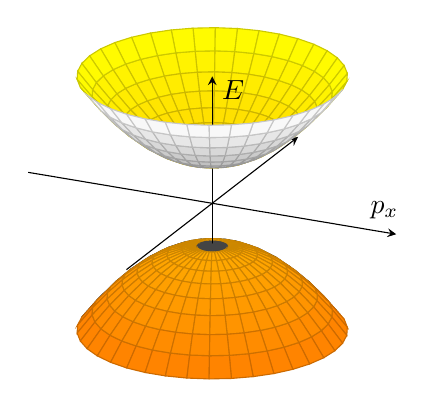
\begin{tikzpicture}
\begin{axis}[
  axis lines=none,
  %xlabel={$p_x$}, ylabel={$p_y$}, zlabel={$E$},
  domain=0:1,
  y domain=0:pi,
  xmin=-1.5, xmax=1.5,
  ymin=-1.5, ymax=1.5, zmin=-1.5, zmax=1.5,
  mesh/interior colormap={blueblack}{color=(orange) color=(yellow)},
  colormap/blackwhite, 
  samples=10,
  samples y=20,
  z buffer=sort,
  ticks=none,
 ]
  \addplot3[surf]  ({x*cos(deg(y))},{x*sin(deg(y))},{+x^2+0.5});
  \addplot3[surf]  ({x*cos(deg(y))},{x*sin(deg(y))},{-x^2-0.5});
\end{axis}

\begin{axis}[
  axis lines=center,
  xlabel={$p_x$}, zlabel={$E$},
  domain=0:1,
  y domain=pi:2*pi,
  xmin=-1.5, xmax=1.5,
  ymin=-1.5, ymax=1.5, zmin=-1.5, zmax=1.5,
  mesh/interior colormap={blueblack}{color=(orange) color=(yellow)},
  colormap/blackwhite, 
  samples=10,
  samples y=20,
  z buffer=sort,
  ticks=none,
 ]
  \addplot3[surf] ({x*cos(deg(y))},{x*sin(deg(y))},{+x^2+0.5});
  \addplot3[surf] ({x*cos(deg(y))},{x*sin(deg(y))},{-x^2-0.5});
\end{axis}

\end{tikzpicture}
\end{center}
}


\newpage
\tableofcontents

%SECTION_NUMBERING
\setcounter{secnumdepth}{2}


\newpage
\section{Useful formulas}

\begin{align}
    \left(\int_{-\infty}^\infty dx e^{-x^2}\right)^2
    &=\int_{-\infty}^\infty dx e^{-x^2} \cdot \int_{-\infty}^\infty dy e^{-y^2}\\
    &=\int_{\mathbb{R}^2}e^{-(x^2+y^2)}dx\,dy\\
    &=\int_0^{2\pi}\int_0^{2\pi}e^{-r^2}r dr \\
    &=-2\pi\left.\frac{e^{-r^2}}{2}\right|^\infty_0=\pi
\end{align}

\subsection{Common integrals}
\begin{align}
    \int_{-\infty}^\infty dx e^{-ax^2}&=\sqrt{\frac{\pi}{a}} \qquad a>0, a\in\mathbb{R}\\
    \int_{-\infty}^\infty dx e^{-ax^2+bx+c}&=\sqrt{\frac{\pi}{a}}e^{\frac{b^2}{4a}+c} \qquad a>0, a,b,c\in\mathbb{R}\\
    \int_{-\infty}^\infty dx e^{iax^2}&=\sqrt{\frac{\pi}{a}}e^{\frac{i\pi}{4}} \qquad a>0, a\in\mathbb{R}
\end{align}
\subsection{Common Fourier integrals}
\begin{align}
    \int_{-\infty}^\infty dy e^{-ay^2}e^{-iby}&=\sqrt{\frac{\pi}{a}}e^{-\frac{b^2}{4a}} \qquad a>0, a,b\in\mathbb{R}\\
    \int_{-\infty}^\infty dy e^{iay^2}e^{-iby}&=\sqrt{\frac{\pi}{a}}e^{\frac{i}{4}\left(\pi-\frac{b^2}{a}\right)} \qquad a>0, a,b\in\mathbb{R}\\
    \int_{-\infty}^\infty dy e^{-(a+ic)y^2}e^{-iby}&=\sqrt{\frac{\pi}{a+ic}}e^{-\frac{b^2}{4(a+ic)}} \qquad a>0, a,b,c\in\mathbb{R}\\
    &=\sqrt{\frac{\pi}{a^2+c^2}}\sqrt{a-ic}\,e^{-\frac{b^2}{4(a^2+c^2)}(a-ic)}
\end{align}

\subsection{Fourier transformation}
Starting from the Fourier integral theorem we have some freedom to distribute the $2\pi$ between back and forth transformation ($a,b\in\mathbb{R}$)
\begin{align}
    F(k)=\sqrt{\frac{|b|}{(2\pi)^{1-a}}}\int_{-\infty}^\infty f(x)e^{ibkx}dx\quad\leftrightarrow\quad f(x)=\sqrt{\frac{|b|}{(2\pi)^{1+a}}}\int_{-\infty}^\infty F(t)e^{-ibkx}dk
\end{align}

\subsection{Delta distribution}
\begin{align}
    \int\delta(x)e^{-ikx}dx&=1\\
    \int e^{ik(x-y)}dk&=2\pi\delta(x-y)
\end{align}
\begin{align}
    \int g(x)\delta(f(x))dx &= \sum_{x_i:f(x_i)=0}\int_{x_i-\epsilon}^{x_i+\epsilon} g(x)\delta(f(x))dx\\
    &= \sum_{x_i}\int_{x_i-\epsilon}^{x_i+\epsilon} g(x)\delta\left(f(x_i)+f'(x_i)(x-x_i)+\frac{1}{2}f''(x_i)(x-x_i)^2+...\right)dx\\
    &= \sum_{x_i}\int_{x_i-\epsilon}^{x_i+\epsilon} g(x)\delta\left(f'(x_i)(x-x_i)\right)dx\\
    &= \sum_{x_i}\int_{(x_i-\epsilon)f'}^{(x_i+\epsilon)f'} g\left(\frac{u}{f'(x_i)}\right)\delta\left(u-f'(x_i)x_i)\right)\frac{1}{f'(x_i)}du\\
    &= \sum_{x_i}\int_{(x_i-\epsilon)|f'|}^{(x_i+\epsilon)|f'|} g\left(\frac{u}{f'(x_i)}\right)\frac{1}{|f'(x_i)|}\delta\left(u-f'(x_i)x_i)\right)du\\
    &= \sum_{x_i} g(x_i)\frac{1}{|f'(x_i)|}
\end{align}
Important restriction: $x_i$ are the {\bf simple} zeros

\subsection{\texorpdfstring{$\Gamma$}{TEXT} function}
\begin{align}
    \Gamma(x)=\int_0^\infty t^{x-1}e^{-t} dx
\end{align}

\subsection{\texorpdfstring{$n$}{TEXT}-dimensional unit spheres}
\begin{align}
    \pi^{n/2}
    &=\left(\int_{-\infty}^\infty dt e^{-t^2}\right)^n\\
    &=\int_{R^n} e^{-|x|^2}dx\\
    &=\int_0^\infty\int_{\omega_n}e^{-r^2}r^{n-1}dr\,ds\\
    &=\int_{\omega_n}ds\cdot\int_0^\infty e^{-r^2}r^{n-1}dr\\
    &=|\omega_n|\cdot\frac{1}{2}\int_0^\infty e^{-\rho}\rho^{\frac{n}{2}-1}d\rho\\
    &=|\omega_n|\cdot\frac{1}{2}\Gamma\left(\frac{n}{2}\right)
\end{align}
Therefore
\begin{align}
|\omega_n| &= \frac{2\pi^{n/2}}{\Gamma\left(\frac{n}{2}\right)}\\
V_n 
&=|\omega_n|\int_0^1r^{n-1}dr\\
&=\frac{|\omega_n|}{n}
\end{align}

\subsection{Laplace operator}
\begin{align}
    \nabla\cdot X&=\frac{1}{\sqrt{|g|}}\partial_i\left(\sqrt{|g|}X^i\right)\\
    (\nabla f)^i&=g^{ij}\partial_jf\\
    \triangle f &= \nabla\cdot\nabla f\\
    &=\frac{1}{\sqrt{|g|}}\partial_i\left(\sqrt{|g|} g^{ij}\partial_jf \right)\\
    &= \sum_i \frac{\partial^2}{\partial x_j^2}
\end{align}

\begin{align}
    \frac{\partial}{\partial x_i}\frac{\partial f}{\partial x_i}
    &=\frac{\partial}{\partial x_i}\left(\frac{\partial y_j}{\partial x_i}\frac{\partial f}{\partial y_j}\right)\\
    &=\frac{\partial y_k}{\partial x_i}\frac{\partial}{\partial y_k}\left(\frac{\partial y_j}{\partial x_i}\frac{\partial f}{\partial y_j}\right)\\
    &=\frac{\partial^2 y_j}{\partial x_i^2}\frac{\partial f}{\partial y_j} + \frac{\partial y_j}{\partial x_i}\frac{\partial y_k}{\partial x_i}\frac{\partial^2 f}{\partial y_j\partial y_k}\\
\end{align}
With $f=f(r)$ and $r=\sqrt{x_1^2+...+x_n^2}$ we have
\begin{align}
    \triangle f(r)
    &=\sum_i \frac{r-x_i \frac{x_i}{r}}{r^2}\frac{\partial f}{\partial r}+\frac{x_i^2}{r^2}\frac{\partial^2 f}{\partial r^2}\\
    &= \frac{nr-r}{r^2}\frac{\partial f}{\partial r}+\frac{r^2}{r^2}\frac{\partial^2 f}{\partial r^2}\\
    &= \frac{(n-1)}{r}\frac{\partial f}{\partial r}+\frac{\partial^2 f}{\partial r^2}
\end{align}



\subsection{Greenfunctions and PDEs}
The Greensfunction $G(x,y)$ for a general PDE $D_x u(x) = f(x)$ is defined by
\begin{align}
    D_x G(x,y) = \delta(x-y).
\end{align}
This means that general solution of the PDE can be expressed as
\begin{align}
    u(x)=\int G(x,y)f(y)dy
\end{align}
because
\begin{align}
    D_x u(x)
    &=D_x \int G(x,y)f(y)dy\\
    &=\int D_x G(x,y)f(y)dy\\
    &=\int \delta(x-y) f(y)dy\\
    &=f(x)
\end{align}

\subsubsection{Poisson equation \texorpdfstring{$\triangle u(x) = f(x)$}{TEXT}}
        
    The $n$-dimensional Fourier transform of $\triangle_x G(x,y) = \delta(x-y)$ and integration by parts gives
    \begin{align}
        \frac{1}{(2\pi)^{n/2}}\int d^nx\,\triangle_x G(x,y) e^{-ikx}&=\frac{1}{(2\pi)^{n/2}}\underbrace{\int d^nx\,\delta(x-y) e^{-ikx}}_{=e^{-iky}}\\
        \frac{1}{(2\pi)^{n/2}}\int d^nx\, G(x,y) (-ik)^2 e^{-ikx}&=\frac{1}{(2\pi)^{n/2}}e^{-iky}\\
        (-ik)^2g(k)&=\frac{1}{(2\pi)^{n/2}}e^{-iky}\\
        &\rightarrow g(k)=-\frac{1}{(2\pi)^{n/2}}\frac{1}{k^2}e^{-iky}
    \end{align}
    we can now use the Fourier transform of the Greensfunction and transform back.
    \begin{itemize}
        \item Case $n=1$: The function has a pole at $k=0$ and the Laurent series is given by
        \begin{align}
            \frac{e^{ik(x-y)}}{k^2}=\frac{1}{k^2}+i(x-y)\frac{1}{k}-\frac{(x-y)^2}{2}-\frac{i(x-y)^3}{6} k + ...
        \end{align}
        with $\text{Res}=i(x-y)$. We can now use the residue theorem to evaluate the integral
        \begin{align}
            G(x,y)&=-\frac{1}{\sqrt{2\pi}}\frac{1}{\sqrt{2\pi}}\int_{-\infty}^\infty dk\; \frac{e^{ik(x-y)}}{k^2}=-\frac{1}{2\pi}\int_{C_1} dk\; \frac{e^{ik(x-y)}}{k^2}\\
            &=-\frac{1}{2\pi}\left(\underbrace{\int_C dk\; \frac{e^{ik(x-y)}}{k^2}}_{=2\pi i\;\text{Res}} - \underbrace{\int_{C_2} dk\; \frac{e^{ik(x-y)}}{k^2}}_{=0}\right)\\
            &=(x-y)
        \end{align}
    
        \begin{center}
        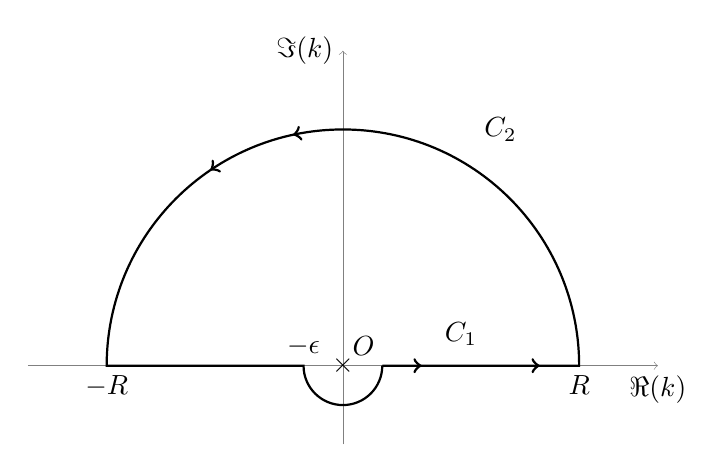
\begin{tikzpicture}[decoration={markings,
            mark=at position 0.5cm with {\arrow[line width=1pt]{>}},
            mark=at position 2cm with {\arrow[line width=1pt]{>}},
            mark=at position 7.85cm with {\arrow[line width=1pt]{>}},
            mark=at position 9cm with {\arrow[line width=1pt]{>}}
            }
            ]
            % The axes
            \draw[help lines,->] (-4,0) -- (4,0) coordinate (xaxis);
            \draw[help lines,->] (0,-1) -- (0,4) coordinate (yaxis);
            
            
            \node at (0,0) {$\times$};
            
            % The path
            %\path[draw,line width=0.8pt,postaction=decorate] (1,0) node[below] {$\epsilon$} -- (2,0) node[below] {$r$} arc (0:180:2) -- (-1,0) arc (180:0:1);
            
            \path[draw,line width=0.8pt,postaction=decorate] (0.5,0)  -- (3,0) node[below] {$R$} arc (0:180:3) node[below] {$-R$} -- (-0.5,0) node[above]{$-\epsilon$} arc (180:360:.5);
            
            % The labels
            \node[below] at (xaxis) {$\Re(k)$};
            \node[left] at (yaxis) {$\Im(k)$};
            \node[above right] {$O$};
            \node at (1.5,.4) {$C_{1}$};
            \node at (2,3) {$C_{2}$};
        \end{tikzpicture}
        \end{center}
        \item Case $n=2$:
        \begin{align}
            G(x,y)&=-\frac{1}{2\pi}\frac{1}{2\pi}\int_{-\infty}^\infty \int_{-\infty}^\infty dk_1 dk_2\; \frac{e^{i(k_1(x_1-y1)+k_2(x_2-y2))}}{k_1^2+k_2^2}\\
            &=-\frac{1}{4\pi^2}\int_{0}^\infty \int_{0}^{2\pi} dk\;d\phi\; \frac{e^{ik |x-y|\cos\phi}}{k^2}k\\
            &=\frac{1}{2\pi}\int_{0}^\infty dk \frac{1}{k}\frac{1}{2\pi}\int_{0}^{2\pi} d\phi\; e^{ik |x-y|\cos\phi}\\
            &=\frac{1}{2\pi}\int_{0}^\infty dk \; \frac{J_0(k|x-y|)}{k}=-\frac{1}{2\pi}\int_{0}^{\infty|x-y|} dk' \; \frac{J_0(k')}{k'}
        \end{align}
        \textcolor{red}{The last integral diverges but we try a nasty trick (?!?)}
        \begin{align}
            \frac{dG}{dx}&=-\frac{1}{2\pi}\frac{d}{dx}\int_{0}^{\infty} dk \; \frac{J_0(k|x-y|)}{k}\\
            &=-\frac{1}{2\pi}\int_{0}^{\infty} dk \; J_1(k|x-y|)\\
            &=-\frac{1}{2\pi}\frac{1}{|x-y|}
        \end{align}
        Now simple integration yields
        \begin{align}
            G(x,y)=-\frac{1}{2\pi}\log(|x-y|)
        \end{align}
        \item Case $n=3$:
        \begin{align}
            G(x,y)&=\frac{1}{(2\pi)^{3}}\int d^3k\,\frac{1}{k^2}e^{ik(x-y)}\\
            &=\frac{1}{(2\pi)^{3}}\int dk\underbrace{\int d\phi}_{=|\omega_2|} \int d\theta\,e^{ik|x-y|\cos\theta}\sin\theta\\
            &=-\frac{1}{(2\pi)^{2}}\int dk \int_{-1}^{+1} e^{ik|x-y|\cos\theta}d\cos\theta\\
            &=-\frac{1}{(2\pi)^{2}}\int dk \frac{e^{ik|x|}-e^{-ik|x-y|}}{ik|x-y|}\\
            &=-\frac{1}{2\pi^2}\int_0^\infty dk \frac{\sin k|x-y|}{k|x-y|}\\
            &=-\frac{1}{2\pi^2}\frac{1}{|x-y|}\int_0^\infty dk' \frac{\sin k'}{k'}\\
            &=-\frac{1}{4\pi}\frac{1}{|x-y|}
        \end{align}
        \item Case $n>3$:
        ...
        
    \end{itemize}

Alternatively we can use the Gauss theorem with $\vec{F}=\nabla_x G(x,y)$
\begin{align}
    \int_V \nabla\cdot \vec{F} dx&=\int_{\partial V} \vec{F}\cdot d\vec{S}\\
    \int_{K_r(y)} \triangle_x G(x,y) dx&=\int_{\partial _{K_r(y)}} \nabla G\cdot d\vec{S}\\
    1&=\frac{\partial G(r,0)}{\partial r}|\omega_{n}|r^{n-1}\\
    \frac{\partial G(r,0)}{\partial r} &= \frac{r^{-n+1}}{|\omega_n|}\\
    G(x,y)&=\left\{\begin{array}{cc}
         \frac{1}{|\omega_2|}\log{|x-y|}                    & n=2  \\
         -\frac{1}{|\omega_n|(n-2)}\frac{1}{|x-y|^{n-2}}    & n\ge3 
    \end{array}\right.
\end{align}

\subsubsection{Helmholtz equation \texorpdfstring{$(\triangle +k^2)u(x)= f(x)$}{TEXT}}
The Greens function is given by $(\triangle_x +k^2)G(x,y)=\delta(x-y)$


\subsubsection{Wave equation \texorpdfstring{$\left(\frac{1}{c^2}\partial_{tt}-\triangle\right) u(x,t)= f(x,t)$}{TEXT}}

\subsubsection{Klein-Gordon equation \texorpdfstring{$\left(\frac{1}{c^2}\partial_{tt}-\triangle+\mu^2\right) u(x,t)= f(x,t)$}{TEXT}}


\subsubsection{Feynman propagator \texorpdfstring{$\left(\triangle-k^2\right) u(x)= f(x)$}{TEXT}}

\subsubsection{Heat equation \texorpdfstring{$\left(\partial_{t}-k\triangle\right) u(x)= f(x)$}{TEXT}}

\subsubsection{Relativistic Heat equation \texorpdfstring{$\left(\partial_{tt}+2\gamma\partial_t-c^2\triangle\right) u(x)= f(x)$}{TEXT}}

\subsection{Probability}

\begin{itemize}
\item Hypothesis $H$: Steve is a librarian
\item Evidence $E$: Steve likes reading books
\end{itemize}
Question: Whats the probability of the hypothesis is true given the evidence is true $P(H|E)$ 
\begin{align}
   P(H|E)\equiv\frac{P(E\cap H)}{P(E)}\qquad P(E|H)\equiv\frac{P(E\cap H)}{P(H)}\\
   \rightarrow\qquad P(H|E)=\frac{P(E|H)\cdot P(H)}{P(E)}=\frac{P(H)\cdot P(E|H)}{P(H)\cdot P(E|H)+ P(\neg H)\cdot P(E|\neg H)}
\end{align}
alternatively
\begin{align}
  P(H|E)&=\frac{\#\text{allPeople}\cdot P(H)\cdot P(E|H)}{\#\text{allPeople}\cdot P(H)\cdot P(E|H)+\#\text{allPeople}\cdot P(\neg H)\cdot P(E|\neg H)}\\
  &=\frac{P(H)\cdot P(E|H)}{P(H)\cdot P(E|H)+ P(\neg H)\cdot P(E|\neg H)}\\
  &=\frac{P(H)\cdot P(E|H)}{P(E)}
\end{align}

\begin{center}
        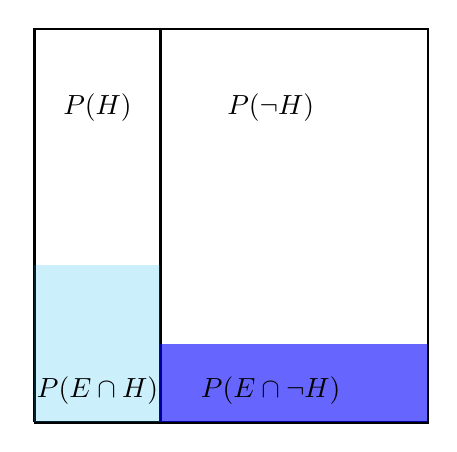
\begin{tikzpicture}
        
            \path[draw,line width=0.8pt] (0,0)  -- (5,0) -- (5,5) -- (0,5) -- (0,0);
            \path[draw,line width=0.8pt] (1.6,0)  -- (1.6,5);
            \path [fill=cyan, fill opacity=0.2] (0,0) rectangle (1.6,2);
            \path [fill=blue, fill opacity=0.6] (1.6,0) rectangle (5,1);
            
            \node at (0.8,4) {$P(H)$};
            \node at (3,4) {$P(\neg H)$};
            \node at (0.8,0.4) {$P(E\cap H)$};
            \node at (3,0.4) {$P(E\cap\neg H)$};
        \end{tikzpicture}
\end{center}


\subsection{Matrices}
\begin{enumerate}
    \item inverse $A^{-1}A=\mathbb{I}$
    \begin{itemize}
        \item therefore $\mathbb{I}=(AB)(B^{-1}A^{-1})\quad\rightarrow\quad (AB)^{-1}=B^{-1}A^{-1}$
    \end{itemize}
    \item Hermitian transpose $A^\dagger = (\overline{A})^T = \overline{A^T}$
        \begin{itemize}
        \item $(AB)^\dagger=B^\dagger A^\dagger$ therefore $\mathbb{I}=(AA^{-1})^\dagger=(A^{-1})^\dagger A^\dagger\quad\rightarrow\quad (A^\dagger)^{-1}=(A^{-1})^\dagger$
        \begin{align}
        \langle x |A y\rangle=\sum_k x_k^* (\vec{A}_{\text{row}k}\cdot\vec{y})=\sum_{k,l} x_k^* A_{kl}y_l\\
        \langle Bx |y\rangle = \sum_k(\vec{B}_{\text{row}k}\cdot \vec{x})^*y_k= \sum_{k,l}B_{kl}^*x_l^*y_k
        \end{align}
    \end{itemize}
    \item Orthorgonal $A^T = A^{-1}$
    \item Unitary $A^\dagger = A^{-1}$
    \item Hermitian $A^\dagger = A$
\end{enumerate}

\subsection{Diagonalization}
Any  matrix $A$ is called diagonalizable if there exists an invertible matrix $S$ such that
\begin{align}
    D_A=S^{-1}AS
\end{align}
is a diagonal matrix. The diagonalizability of $A$ is equivalent to the fact that the $\{\vec{v}_i\}$ are all linearly independent.

To find $S$ and $D_A$ one has to find the eigensystem $\{\lambda_i,\vec{v}_i\}$ with $A\vec{v}_i=\lambda_i\vec{v}_i$. Then $D_AS$ and $S$ can be written as $S=(\vec{v}_1,...,\vec{v}_n)$ and $D_A=\text{diag}(\lambda_1,...,\lambda_n)$ because $AS=(A\vec{v}_1,...,A\vec{v}_n)=(\lambda_1\vec{v}_1,...,\lambda_n\vec{v}_n)=SD_A$.

\subsection{Functional derivatives}
Let $F[\phi]$ a functional, i.e. a mapping from a Banach space $\mathcal{M}$ to the field of real or complex numbers. The functional (Frechet) derivative $\delta F[\phi]/\delta\phi$ is defined by
\begin{align}
    \delta F
    &=\int dx \frac{\delta F[\phi]}{\delta\phi(x)}\cdot\delta\phi(x)\\
    &=\int dx \frac{\delta F[\phi]}{\delta\phi(x)}\cdot\epsilon\delta(x-y)\\
    &=\epsilon\frac{\delta F[\phi]}{\delta\phi(y)}\\
    &=F[\phi+\epsilon\delta(x-y)]-F[\phi]
\end{align}
which means
\begin{align}
    \frac{\delta F[\phi]}{\delta\phi[y]}&=\lim_{\epsilon\rightarrow0}\frac{F[\phi+\epsilon\delta(x-y)]-F[\phi]}{\epsilon}\\
    F[\phi+\epsilon\delta(x-y)]&=F[\phi]+\epsilon\frac{\delta F[\phi]}{\delta\phi(y)}\\
    &=F[\phi]+\epsilon\int dx \frac{\delta F[\phi]}{\delta\phi(x)}\cdot\delta(x-y)
\end{align}
\begin{itemize}
    \item Product rule $F[\phi]=G[\phi]H[\phi]$
    \begin{align}
        \frac{\delta F[\phi]}{\delta\phi(x)}
        &=\frac{\delta(G[\phi]H[\phi])}{\delta\phi}\\
        &=\lim_{\epsilon\rightarrow0}\frac{G[\phi+\epsilon\delta(x-y)]H[\phi+\epsilon\delta(x-y)]-G[\phi]H[\phi]}{\epsilon}\\
        &=\lim_{\epsilon\rightarrow0}\frac{\left(G[\phi]+\epsilon\frac{\delta G}{\delta\phi}\right)\left(H[\phi]+\epsilon\frac{\delta H}{\delta\phi}\right)-G[\phi]H[\phi]}{\epsilon}\\
        &=\lim_{\epsilon\rightarrow0}\frac{G[\phi]H[\phi]+\epsilon G[\phi]\frac{\delta H}{\delta\phi}+\frac{\delta G}{\delta\phi}H[\phi]+\epsilon^2\frac{\delta G}{\delta\phi}\frac{\delta H}{\delta\phi}-G[\phi]H[\phi]}{\epsilon}\\
        &=G[\phi]\frac{\delta H[\phi]}{\delta\phi(x)}+\frac{\delta G[\phi]}{\delta\phi(x)}H[\phi]
    \end{align}
    \item Chain rule $F[G[\phi]]$
    \begin{align}
        \delta F
        &=\int dx \frac{\delta F[G[\phi]]}{\delta\phi(x)} \delta\phi(x)\\
        \delta G
        &=\int dy \frac{\delta G[\phi]}{\delta\phi(y)} \delta\phi(y)\\
        \delta F
        &=\int dz \frac{\delta F[G]}{\delta G(z)} \delta G(z)\\
        &=\int dz \frac{\delta F[G]}{\delta G(z)} \int dy \frac{\delta G[\phi]}{\delta\phi(y)} \delta\phi(y) \\
        &=\int dy \underbrace{\int dz \frac{\delta F[G]}{\delta G(z)} \frac{\delta G[\phi]}{\delta\phi(y)}}_{=\frac{\delta F[G[\phi]]}{\delta\phi(y)}} \;\delta\phi(y) \\
        \frac{\delta F[G[\phi]]}{\delta\phi(y)}
        &=\int dz \frac{\delta F[G]}{\delta G(z)} \frac{\delta G[\phi]}{\delta\phi(y)}
    \end{align}
    \item Chain rule (special case) $F[g[\phi]]$
    \begin{align}
        \frac{\delta F[g[\phi]]}{\delta\phi(y)}
        &=...\\
        &=\frac{\delta F}{\delta g(\phi(y))} \frac{d g(\phi)}{d\phi(y)}
    \end{align}
\end{itemize}
Some examples
\begin{enumerate}
    \item $F[\phi]=\int dx \phi(x)\delta(x)$
    \begin{align}
        \frac{\delta F[\phi]}{\delta\phi(y)}
           &=\lim_{\epsilon\rightarrow0}\frac{1}{\epsilon}\left(\int dx(\phi(x)+\epsilon\delta(x-y))\delta(x))-\int
        dx\,\phi(x)\delta(x)\right)\\
        &=\int dx\,\delta(x-y))\delta(x)\\
       &=\delta(y)
    \end{align}
    \item $F[\phi]=\int dx \phi(x)$
    \begin{align}
        \frac{\delta F[\phi]}{\delta\phi(y)}
        &=\lim_{\epsilon\rightarrow0}\frac{1}{\epsilon}\left(\int dx(\phi(x)+\epsilon\delta(x-y)))-\int dx\,\phi(x)\right)\\
        &=\int dx\,\delta(x-y)\\
        &=1
    \end{align}
    \item $F_x[\phi]=\phi(x)$
    \begin{align}
        \frac{\delta \phi(x)}{\delta\phi(y)}=\frac{\delta F_x[\phi]}{\delta\phi(y)}
        &=\lim_{\epsilon\rightarrow0}\frac{1}{\epsilon}\left((\phi(x)+\epsilon\delta(x-y))-\phi(x)\right)\\
        &=\delta(x-y)
    \end{align}
    \item $F[\phi]=\int dx \phi(x)^n$
    \begin{align}
        \frac{\delta F[\phi]}{\delta\phi(y)}
        &=\lim_{\epsilon\rightarrow0}\frac{1}{\epsilon}\left(\int dx(\phi(x)+\epsilon\delta(x-y)))^n-\int dx\,\phi(x)^n\right)\\
        &=\int dx\,n\phi(x)^{n-1}\delta(x-y)\\
        &=n\phi(y)^{n-1}
    \end{align}
    \item $F[\phi]=\int dx \left(\frac{\phi(x)}{dx}\right)^n$
    \item $F_y[\phi]=\int dz K(y,z)\phi(z)$
    \begin{align}
        \frac{\delta F_y[\phi]}{\delta\phi(x)}
           &=\lim_{\epsilon\rightarrow0}\frac{1}{\epsilon}\left(\int dz(K(y,z)(\phi(z)+\epsilon\delta(z-x)) -\int dz K(y,z)\phi(z)\right)\\
           &=\int dz\,K(y,z)\delta(z-x)\\
           &=K(y,x)
    \end{align}
    \item $F_x[\phi]=\nabla\phi(x)$
    \begin{align}
        \frac{\delta F[\phi]}{\delta\phi(y)}
        &=\lim_{\epsilon\rightarrow0}\frac{1}{\epsilon}\left( \nabla_x(\phi(x)+\epsilon\delta(x-y)) - \nabla_x\phi(x)\right)\\
        &=\nabla_x\delta(x-y)
    \end{align}
    \item $F[\phi]=g\left(G[\phi(x)]\right)$
    \begin{align}
        \frac{\delta F[\phi]}{\delta\phi(y)}
        &=\lim_{\epsilon\rightarrow0}\frac{1}{\epsilon}g(G[\phi(x)+\epsilon\delta(x-y)])-g(G[\phi(x)])\\
        &=\lim_{\epsilon\rightarrow0}\frac{1}{\epsilon}g(G[\phi(x)]+\epsilon\frac{\delta G}{\delta \phi})-g(G[\phi(x)])\\
        &=\lim_{\epsilon\rightarrow0}\frac{1}{\epsilon}g(G[\phi(x)])+g' \epsilon\frac{\delta G}{\delta \phi}-g(G[\phi(x)])\\
        &=\frac{\delta G}{\delta \phi}g'(G[\phi(x)])
    \end{align}
    
\end{enumerate}

\subsection{Space hierarchy}
\begin{enumerate}
    \item K-Vector space $(K,\oplus,\odot)$ 
        \begin{itemize}
            \item set $V$, field $K$ with $(K,+,\cdot)$
            \item vector addition $\oplus: V\times V\rightarrow V$
            \item scalar multiplication $\odot: K\times V\rightarrow V$
        \end{itemize}
    \item Topological vector space
        \begin{itemize}
            \item K-vector space
            \item continuous (smooth) vector addition and scalar multiplication
        \end{itemize}
    \item Metric (vector) space $(M,d)$
        \begin{itemize}
            \item set $M$, metric $d: M\times M\rightarrow \mathbb{R}$
            \item $d(x,y)=0 \Leftrightarrow x=y$
            \item $d(x,y)=d(y,x)$
            \item $d(x,y)+d(y,z) \ge d(x,z)$
            \item from the requirements above follows $d(x,y)\ge0$
        \end{itemize}
    \item Normed vector space $(V,\|\cdot\|)$
        \begin{itemize}
            \item K-vector space $V$, norm $\|\cdot\|: V\rightarrow \mathbb{R}$
            \item Typically $K\in(\mathbb{R}, \mathbb{C})$ to have a definition of $|\lambda|$
            \item $\|x\|\ge0$
            \item $\|x\|=0 \Leftrightarrow x=0$
            \item $\|\lambda x\|=|\lambda| \|x\|$ with $\lambda\in K$
            \item $\|x\|+\|y\|\ge\|x+y\|$
            \item with $d(x,y):=\|x-y\|$ every normed vector space has also a metric
            \item a metric does NOT induce a always norm as the linearity/homogeneity of the norm is not guaranteed 
        \end{itemize}
    \item Banach space (complete normed vector space)
        \begin{itemize}
            \item normed K-vector space $(V,\|\cdot\|)$ with $K\in(\mathbb{R}, \mathbb{C})$
            \item completeness: every Cauchy sequence converges (with the metric induced by the norm) to a well defined limit
            \item if the space is just a metric space (without a norm) the space is called Cauchy space
        \end{itemize}
    \item Hilbert space (complete vector space with a scalar product)
        \begin{itemize}
            \item K-vector space $V$ with $K\in(\mathbb{R}, \mathbb{C})$
            \item scalar product $\langle\cdot,\cdot\rangle:V\times V\rightarrow K$
            \item $\langle \lambda x_1+x_2,y\rangle = \langle \lambda x_1,y\rangle + \langle \lambda x_2,y\rangle$
            \item $\langle \lambda x,y\rangle = \lambda\langle x,y\rangle$ for $\lambda\in K$
            \item $\langle x,y\rangle=\overline{\langle y,x\rangle}$ which implies $\langle x,x\rangle \in \mathbb{R}$
            \item $\langle x,x\rangle>0$
            \item $\langle x,x\rangle=0\Leftrightarrow x=0$
            \item completeness: every Cauchy sequence converges (with the metric induced by the norm which is itself induced by the scalar product) to a well defined limit
            \item without completeness the space is called Pre-Hilbert space
        \end{itemize}
\end{enumerate}


\subsection{Tensors}
\begin{itemize}
\item For a vector $\mathbf{A}$ the expression $\mathbf{A}^2$ is the squared distance between tip and tail.
\item The inner product of two vectors can then be defined by the parallelogram law
\begin{align}
    \mathbf{A}\cdot\mathbf{B}\equiv\frac{1}{4}\left[(\mathbf{A}+\mathbf{B})^2-(\mathbf{A}-\mathbf{B})^2\right]
\end{align}
\item A rank-$n$ tensor $\mathbf{T}=\mathbf{T}(\_,\_,\_)$ is real-valued linear function of $n$ vectors.
\begin{align}
    \mathbf{T}(\alpha\mathbf{A}+\mu\mathbf{B},\mathbf{C},\mathbf{D})=\alpha\mathbf{T}(\mathbf{A},\mathbf{C},\mathbf{D})+\beta\mathbf{T}(\mathbf{B},\mathbf{C},\mathbf{D})
\end{align}
\item Metric tensor
\begin{align}
    \mathbf{g}(\mathbf{A},\mathbf{B})\equiv\mathbf{A}\cdot\mathbf{B}
\end{align}
\item A vector is a tensor of rank one 
\begin{align}
    \mathbf{A}(\mathbf{C})\equiv\mathbf{A}\cdot\mathbf{C}
\end{align}
\item Tensor product 
\begin{align}
    \mathbf{A}\otimes\mathbf{B}\otimes\mathbf{C}(\mathbf{E},\mathbf{F},\mathbf{G})\equiv\mathbf{A}(\mathbf{E})\mathbf{B}(\mathbf{F})\mathbf{C}(\mathbf{G})=(\mathbf{A}\cdot\mathbf{E})(\mathbf{B}\cdot\mathbf{F})(\mathbf{C}\cdot\mathbf{G})
\end{align}
\item Contraction
\begin{align}
    \text{1\&3 contraction}(\mathbf{A}\otimes\mathbf{B}\otimes\mathbf{C}\otimes\mathbf{D})\equiv(\mathbf{A}\cdot\mathbf{C})\mathbf{B}\otimes\mathbf{D}
\end{align}
\item Orthogonal basis
\begin{align}
    \mathbf{e}_j\cdot\mathbf{e}_k=\delta_{jk}
\end{align}
\item Component expansion
\begin{align}
    \mathbf{A}=A_j\mathbf{e}_j\quad&\rightarrow\quad A_j=\mathbf{A}(\mathbf{e}_j)=\mathbf{A}\cdot\mathbf{e}_j\\
    \mathbf{T}=T_{abc}\mathbf{e}_a\otimes\mathbf{e}_b\otimes\mathbf{e}_c\quad&\rightarrow\quad T_{ijk}=\mathbf{T}(\mathbf{e}_i,\mathbf{e}_j,\mathbf{e}_k)\\
    \text{1\&3 contraction}(\mathbf{R})\quad&\rightarrow\quad R_{ijik}\\
    \mathbf{g}\quad&\rightarrow\quad g_{jk}=\mathbf{g}(\mathbf{e}_j,\mathbf{e}_k)=\mathbf{e}_j\cdot\mathbf{e}_k=\delta_{jk}
\end{align}
\end{itemize}


\newpage
\section{Primer special relativity}
Definition of line element
\begin{align}
    ds^2 &= dx^\mu dx_\nu = \eta_{\mu\nu}dx^\mu dx^\nu\\
        &= dx^T\eta dx
\end{align}
Definition of Lorentz transformation
\begin{align}
    dx^\mu = \Lambda^\mu_{\;\nu}dx^\nu
\end{align}
By postulate the line element $ds$ is invariant under Lorentz transformation
\begin{align}
    ds^2 &= \eta_{\mu\nu}dx^\mu dx^\nu\\
    &\stackrel{!}{=} \eta_{\alpha\beta}\Lambda^\alpha_{\;\mu}dx^\mu \Lambda^\beta_{\;\nu}dx^\nu\quad\rightarrow\quad \eta_{\mu\nu} = \eta_{\alpha\beta}\Lambda^\alpha_{\;\mu} \Lambda^\beta_{\;\nu}
\end{align}
or analog
\begin{align}
    ds^2 &= dx^T\eta dx\\
    &\stackrel{!}{=} (\Lambda dx)^T\eta (\Lambda dx)\\
    &= dx^T\Lambda^T\eta \Lambda dx\quad\rightarrow\quad \eta = \Lambda^T\eta\Lambda
\end{align}
Observation with the eigentime $d\tau=ds/c$ and 3-velocity $dx^i = v^i dt$
\begin{align}
    \frac{ds^2}{d\tau^2}=c^2&=c^2\frac{dt^2}{d\tau^2}-\frac{dx^i}{dt}\frac{dx_i}{dt}\left(\frac{dt}{d\tau}\right)^2\\
    1&=\frac{dt^2}{d\tau^2}\left(1-\frac{v^iv_i}{c^2}\right)\quad\rightarrow\quad\frac{dt}{d\tau}\equiv\gamma=\left(\sqrt{1-\frac{v^2}{c^2}}\right)^{-1}
\end{align}
Definition of 4-velocity with 3-velocity $d\vec{x} = \vec{v} dt$
\begin{align}
    u^\mu\equiv\frac{dx^\mu}{d\tau}&=\frac{dx^\mu}{dt}\frac{dt}{d\tau}=\quad\rightarrow\quad u^\mu u_\mu=\eta_{\mu\nu}\frac{dx^\mu}{d\tau} \frac{dx^\nu}{d\tau}=\frac{ds^2}{d\tau^2}=c^2\\
    &=(c,\vec{v})\gamma
\end{align}
Object moving in $x$ direction with $v$ meaning $dx=v\cdot dt$ compared to
rest frame $dx'=0$
\begin{align}
    c^2dt'^2=ds^2 &= c^2dt^2- v^2 dt^2\\
    &=c^2dt^2\left(1-\frac{v^2}{c^2}\right)\\
    dt'=\frac{ds}{c}\equiv d\tau&=dt\sqrt{1-\frac{v^2}{c^2}}=\frac{dt}{\gamma}
\end{align}
Definition 4-momentum (using the 3-momentum $\vec{p}=\gamma m\vec{v}$)
\begin{align}
    p^\mu \equiv mu^\mu=(\gamma mc,\gamma m\vec{v})=\left(\frac{E_p}{c},\vec{p}\right)\quad&\rightarrow\quad p^\mu p _\mu=m^2u^\mu u_\mu=m^2c^2\\
    &\rightarrow\quad (p^0)^2-p^ip_i=m^2c^2\\
    &\rightarrow\quad p^0=\sqrt{m^2c^2+\vec{p}^2}\\
    &\rightarrow\quad E_p=\sqrt{m^2c^4+\vec{p}^2c^2}\\
    &\qquad\qquad=\frac{mc^2}{\sqrt{1-\frac{\vec{v}^2}{c^2}}}
\end{align}
First we observe
\begin{align}
    \eta_{\mu\nu} &= \eta_{\alpha\beta}\Lambda^\alpha_{\;\mu} \Lambda^\beta_{\;\nu}\\
    \det(\eta)&=\det(\Lambda)^2\det(\eta)\\
    1&=\det(\Lambda)^2.
\end{align}
Now we see
\begin{align}
    \Lambda_\gamma^{\;\nu}\Lambda^\gamma_{\;\mu}&=\eta_{\alpha\gamma}\eta^{\nu\beta}\Lambda^\alpha_{\;\beta} \Lambda^\gamma_{\;\mu}\\
    &=\eta^{\nu\beta}(\eta_{\alpha\gamma}\Lambda^\alpha_{\;\beta} \Lambda^\gamma_{\;\mu})\\
    &=\eta^{\nu\beta}\eta_{\beta\mu}\\
    &=\delta^\nu_{\;\mu}
\end{align}
which means in matrix notation $\Lambda_\gamma^{\;\nu}=(\Lambda^{-1})^\nu_{\;\gamma}$.
General transformation laws for tensors of first order
\begin{align}
    V'^\alpha&=\Lambda^\alpha_{\;\beta}V^\beta\\
    \eta_{\alpha\mu}V'^\alpha&=\eta_{\alpha\mu}\Lambda^\alpha_{\;\beta}V^\beta=\eta_{\alpha\mu}\Lambda^\alpha_{\;\beta}(\eta^{\nu\beta}V_\nu)\\
    V'_\mu&=\Lambda_\mu^{\;\nu}V_\nu\\
    &\rightarrow\quad \Lambda_\mu^{\;\nu} = \eta_{\alpha\mu}\eta^{\nu\beta}\Lambda^\alpha_{\;\beta}
\end{align}
and second order
\begin{align}
    T'^{\alpha\beta}&=\Lambda^\alpha_{\;\mu}\Lambda^\beta_{\;\nu}T^{\mu\nu}\\
    \eta_{\alpha\delta}\eta_{\beta\gamma}T'^{\alpha\beta}&=\eta_{\alpha\delta}\eta_{\beta\gamma}\Lambda^\alpha_{\;\mu}\Lambda^\beta_{\;\nu}T^{\mu\nu}=\eta_{\alpha\delta}\eta_{\beta\gamma}\Lambda^\alpha_{\;\mu}\Lambda^\beta_{\;\nu}(\eta^{\mu\rho}\eta^{\nu\sigma} T_{\rho\sigma})\\
    T'_{\delta\gamma}&=\Lambda_\delta^{\;\rho}\Lambda_\gamma^{\;\sigma}T_{\rho\sigma}.
\end{align}
The general transformation is therefore given by
\begin{align}
    {T'_{\mu_1\mu_2...}}^{\nu_1\nu_2...}={\Lambda_{\mu_1}}^{\rho_1}{\Lambda_{\mu_2}}^{\rho_2}... {\Lambda^{\nu_1}}_{\sigma_1}{\Lambda^{\nu_2}}_{\sigma_2}... {T'_{\rho_1\rho_2...}}^{\sigma_1\sigma_2...}
\end{align}
There exist two invariant tensors
\begin{align}
    \eta'_{\mu\nu} 
    &=\eta_{\alpha\beta}\Lambda^\alpha_{\;\mu} \Lambda^\beta_{\;\nu}
    =\Lambda_{\beta\mu} \Lambda^\beta_{\;\nu}
    =\eta_{\mu\sigma}\Lambda_{\beta}^{\;\sigma} \Lambda^\beta_{\;\nu}
    =\eta_{\mu\sigma}\delta^\sigma_{\;\nu}
    =\eta_{\mu\nu}\\
    {\epsilon'}^{\mu\nu\rho\sigma}
    &=\Lambda^\mu_{\;\alpha}\Lambda^\nu_{\;\beta}\Lambda^\rho_{\;\gamma}\Lambda^\sigma_{\;\delta}{\epsilon'}^{\alpha\beta\gamma\delta}\equiv \epsilon^{\mu\nu\rho\sigma} \det(\Lambda)=\pm \epsilon^{\mu\nu\rho\sigma}
\end{align}
Due to the possibility of the minus sign the Levi-Civita symbol $\epsilon$ is sometimes called pseudo-tensor.

\section{Groups}
\subsection{Overview}
\begin{table}[!h]
    \centering
    \begin{tabular}{c | c c c c c c}
        $\mathbb{F}$    & GL($n,\mathbb{F}$)    & SL($n,\mathbb{F}$) & U($n$) & SU($n$) & O($n$)     & SO($n$)     \\ \hline\hline
        $\mathbb{R}$    & $n^2$                 & $n^2-1$            & -      & -       & $n(n-1)/2$ & $n(n-1)/2$  \\
        $\mathbb{C}$    & $2n^2$                & $2(n^2-1)$         & $n^2$  & $n^2-1$ & $n(n-1)$   & $n(n-1)$    \\
    \end{tabular}
    \caption{Dimensions of common Lie groups (number of independent real parameters)}
    \label{tab:my_label}
\end{table}
Observation: $\text{dim}(\text{SO}(n,\mathbb{F}))=\text{dim}(\text{O}(n,\mathbb{F}))$  - sign that SO($n$) is not connected

\subsection{SO(2)}
There are infinitely many (non-equivalent) 1-dimensional standard irreps
\begin{align}
    D^{k}(\alpha)=e^{-ik\alpha},\,k=0,\pm1,\pm2,...
\end{align}

\subsection{SO(3)}

\subsection{SU(2)}
Finite dimensional irreps of the Lorentz group are labeled by $l$ with
\begin{align}
    l &\in \left\{0,\frac{1}{2},1,\frac{3}{2},2,...\right\}.
\end{align}
and have dimension $2l+1$. For two irreps with $l\ge m$ the tensor product representations decomposes as ({\sc Clebsch-Gordan} decomposition)
\begin{align}
    V_l \otimes V_m &\cong \bigoplus_{j=l-m}^{l+m} V_j\\
    &=V_{l+m}\oplus V_{l+m-1}\oplus ... \oplus V_{l-m+1}\oplus V_{l-m}\\
    \text{dim}(V_l \otimes V_m)&=(2l+1)(2m+1)\\
    \text{dim}(V_{l+m} \oplus ...\oplus V_{l-m})&=\sum_{k=0}^{2m}2[(l-m)+k]+1\\
    &=(2m+1)[2(l-m)+1]+2\frac{2m(2m+1)}{2}\\
    &=(2m+1)(2l+1)
\end{align}

\subsection{SU(3)}

\subsection{Lorentz group O(1,3)}
There are the obvious tensor representations for tensors of first and second order
\begin{align}
    [D(\Lambda)]^\alpha_{\;\beta}=\Lambda^\alpha_{\;\beta}\quad &\rightarrow\quad V^\alpha = [D(\Lambda)]^\alpha_{\;\beta} V^\beta=\Lambda^\alpha_{\;\beta} V^\beta\\
    [D(\Lambda)]_{\alpha\beta}^{\;\;\gamma\delta}=\Lambda_\alpha^{\;\gamma}\Lambda_\beta^{\;\delta}\quad&\rightarrow\quad T_{\alpha\beta} = [D(\Lambda)]_{\alpha\beta}^{\;\;\gamma\delta} T_{\gamma\delta}=\Lambda_\alpha^{\;\gamma}\Lambda_\beta^{\;\delta}T_{\gamma\delta}
\end{align}
which are 4 and 16 dimensional.

Infinitesimal Lorentz transformations can be written as
\begin{align}
    \Lambda^\alpha_{\;\beta}=\delta^\alpha_{\;\beta}+\omega^\alpha_{\;\beta}\qquad(|\omega^\alpha_{\;\beta}|\ll 1).
\end{align}
The first order approximation gives an additional restriction
\begin{align}
    \eta_{\mu\nu} &= \eta_{\alpha\beta}\Lambda^\alpha_{\;\mu}\Lambda^\beta_{\;\nu}=\eta_{\alpha\beta}(\delta^\alpha_{\;\mu}+\omega^\alpha_{\;\mu})(\delta^\beta_{\;\nu}+\omega^\beta_{\;\nu})=\eta_{\mu\nu}+\eta_{\mu\beta}\omega^\beta_{\;\nu}+\eta_{\alpha\nu}\omega^\alpha_{\;\mu}\\
    &\rightarrow \omega_{\mu\nu}=-\omega_{\nu\mu}
\end{align}
which implies six independent components. As the four dimensional representation of the infinitesimal transformation is close to unity it can then be written as
\begin{align}
    D(\Lambda)=D(1+\omega)=1+\frac{1}{2}\omega^{\alpha\beta}\sigma_{\alpha_\beta}
\end{align}
where the six $\omega$ components correspond to the six matrices $\sigma_{01},\sigma_{02},\sigma_{03},\sigma_{12},\sigma_{13},\sigma_{23}$ which are the generators of the group.


Finite dimensional irreps of the Lorentz group are labeled by two parameters $(\mu,\nu)$ with
\begin{align}
    \mu,\nu &\in \left\{0,\frac{1}{2},1,\frac{3}{2},2,...\right\}.
\end{align}
and have dimension $(2\mu+1)(2\nu+1)$
\begin{align*}
    M^2&=\mu(\mu+1)\\
    N^2&=\nu(\nu+1)\\
    j  &\in |\mu-\nu|, ..., (\mu+\nu)
\end{align*}


\begin{center}
 \begin{tabular}{c c c l} 
 \hline
 irrep & dim & $j$ & example \\ [0.5ex] 
 \hline\hline
 $(0,0)$                        & 1 & 0 & Scalar \\  [0.5ex]
 $(\frac{1}{2},0)$              & 2 & $\frac{1}{2}$ & Left-handed Weyl spinor \\  [0.5ex]
 $(0,\frac{1}{2})$              & 2 & $\frac{1}{2}$ & Right-handed Weyl spinor \\  [0.5ex]
 $(\frac{1}{2},\frac{1}{2})$    & 4 & 0,1 & 4-Vector $A^\mu$ \\  [0.5ex]
 $(1,0)$                        & 3 & 1 & Self-dual 2-form \\  [0.5ex]
 $(0,1)$                        & 3 & 1 & Anti-self-dual 2-form \\  [0.5ex]
 $(1,1)$                        & 9 & 0,1,2 & Traceless symmetric $2^\text{nd}$ rank tensor \\ \hline  \\ [0.5ex]
  \hline
 rep & dim & j & example \\ [0.5ex] 
 \hline\hline
 $(\frac{1}{2},0)\oplus(0,\frac{1}{2})$& - & - & Dirac bispinor $\psi^\alpha\quad \alpha\in\{1,2,3,4\}$ \\  [0.5ex]
 $(\frac{1}{2},\frac{1}{2})\otimes\left[(\frac{1}{2},0)\oplus(0,\frac{1}{2})\right]$& - & - & Rarita-Schwinger field $\psi^\alpha\quad \alpha\in\{1,2,3,4\}$ \\  [0.5ex]
  $(0,1)\oplus(0,1)$& - & - & Parity invariant field of 2-forms\\ \hline \\ [0.5ex]
\end{tabular}
\end{center}



\newpage
\section{Mathematical}

\subsection{{\sc Andrews} - Number theory}
\subsubsection{Problem 1.1}
Lets cut the chase
\begin{align}
\frac{n(n+1)(2n+1)}{6}+(n+1)^2
&=(n+1)\frac{n(2n+1)+6(n+1)}{6}\\
&=\frac{(n+1)}{6}(2n^2+7n+6)\\
&=\frac{(n+1)}{6}(n+2)(2n+3)\\
&=\frac{(n+1)}{6}(n+2)(2(n+1)+1)\\
&=\frac{(n+1)(n+2)(2(n+1)+1)}{6}\\
\end{align}

\subsection{{\sc Bender, Orszag} - Advanced Mathematical Methods for Scientists and Engineers}
\subsubsection{Problem 1.1}
\begin{enumerate}
    \item $y'=e^{x+y}$
    \begin{align}
        \int\frac{dy}{e^y}&=\int e^xdx\\
        -e^{-y}&=e^x+c\\
        y&=-\log\left(-e^x+c\right)
    \end{align}
    \item $y'=xy+x+y+1$
    \begin{align}
        \frac{dy}{y+1}&=x+1\\
        \log y+1&=\frac{x^2}{2}+x+c\\
        y&=c'e^{x/2(x+2)}-1
    \end{align}
\end{enumerate}
\subsubsection{Problem 1.2}
$y''=yy'/x$
\begin{enumerate}
    \item Equidimensional-in-$s$ equation
    \begin{align}
        x&=e^t\\
        \frac{d}{dx}&=\frac{dt}{dx}\frac{d}{dt}\\
        &=\frac{1}{x}\frac{d}{dt}\\
        \frac{d^2}{dx^2}&=\frac{dt}{dx}\frac{d}{dt}\left(\frac{1}{x}\frac{d}{dt}\right)\\
        &=\frac{1}{x}\left(-\frac{1}{x^2}x\frac{d}{dt}+\frac{1}{x}\frac{d^2}{dx^2}\right)\\
        &=\frac{1}{x^2}\left(-\frac{d}{dt}+\frac{d^2}{dt^2}\right)
    \end{align}
    now with $y=y(t)$
    \begin{align}
        -y'+y''=yy'
    \end{align}
    \item Autonomous equation
    \begin{align}
        y'&\equiv u(y)\\
        y''&=\frac{du}{dy}\frac{dy}{dt}=\dot u y'
    \end{align}
    now with $u=u(y)$
    \begin{align}
        -u+\dot u u&=y u\\
        \dot u&=y+1
    \end{align}
    \item integration
    \begin{align}
        u=\frac{y^2}{2}+y+c_0
    \end{align}
    \item resubstitution I (with $\tan z = i\frac{e^{-iz}-e^{iz}}{e^{-iz}+e^{iz}}$)
    \begin{align}
        y'&=\frac{y^2}{2}+y+c_0\\
        t+c_3&=\int\frac{dy}{y^2/2+y+c_0}\\
        &=2\frac{1}{2\sqrt{1-2c_0}}\int dy\left(-\frac{1}{y+1+\sqrt{1-2c_0}}+\frac{1}{y+1-\sqrt{1-2c_0}}\right)\\
        &=\frac{1}{\sqrt{1-2c_0}}\left(-\log\left[y+1+\sqrt{1-2c_0}\right]+\log\left[y+1-\sqrt{1-2c_0}\right]\right)\\
        &=\frac{1}{\sqrt{1-2c_0}}\log\frac{y+1-\sqrt{1-2c_0}}{y+1+\sqrt{1-2c_0}}\\
        &=\frac{1}{\sqrt{1-2c_0}}\log\frac{-i\sqrt{1-2c_0}\left(-i+\frac{i(y+1)}{\sqrt{1-2c_0}}\right)}{i\sqrt{1-2c_0}\left(-i-\frac{i(y+1)}{\sqrt{1-2c_0}}\right)}\\
        &=\frac{1}{\sqrt{1-2c_0}}\log\frac{-\left(-i+\frac{i(y+1)}{\sqrt{1-2c_0}}\right)}{\left(-i-\frac{i(y+1)}{\sqrt{1-2c_0}}\right)}\\
        &=\frac{2}{\sqrt{1-2c_0}}\log\sqrt{-\frac{-i+\frac{i(y+1)}{\sqrt{1-2c_0}}}{-i-\frac{i(y+1)}{\sqrt{1-2c_0}}}}\\
        &=\frac{2}{i\sqrt{1-2c_0}}\arctan\left(-\frac{i(y+1)}{\sqrt{1-2c_0}}\right)
    \end{align}
    \item resubstitution II
    \begin{align}
        \log x+c_3&=\frac{2}{i\sqrt{1-2c_0}}\arctan \frac{y+1}{i\sqrt{1-2c_0}}\\
        \tan\left[\frac{\sqrt{2c_0-1}}{2}(\log x+c_3)\right]&=\frac{y+1}{\sqrt{2c_0-1}}\\
        y&=\sqrt{2c_0-1}\tan\left[\frac{\sqrt{2c_0-1}}{2}(\log x+c_3)\right]-1\\
        y&=2c_1\tan\left[c_1\log x+c_2\right]-1
    \end{align}

\end{enumerate}
This solution has poles at
\begin{align}
    \log x_P =\frac{\pi/2+k\pi-c_2}{c_1}
\end{align}
while the special solution $-2/(c_4+\log x)-1$ has a pole at
\begin{align}
    \log x_P=-c_4
\end{align}
???

\subsubsection{Problem 1.10}
With $y=e^{rx}$ the equation $y'''-3y''+3y'-y=0$ becomes
\begin{align}
    r^3-3r^2+3r-1&=0\\
    (r-1)^3&=0
\end{align}
then $y=c_1e^x+c_2xe^x+c_3x^2e^x$.

\subsubsection{Problem 1.11}
We guess $y_1=e^{-x}$ and have another guess  $y_2=e^{-x}u(x)$ we see
\begin{align}
    r^{-x}\left(u''+xu'\right)&=0\\
    v'+xv&=0\\
    v&=c_0e^{-x^2/2}\\
    u&=c_1\text{erf}\left(\frac{x}{\sqrt{2}}\right)+c_2
\end{align}
and therefore $y=c_3e^{-x}+c_4e^{-x}\left[\text{erf}\left(\frac{x}{\sqrt{2}}\right)+c_5\right]$

\subsection{{\sc Arnol'd} - A mathematical trivium}
\subsubsection{Problem 4}
\begin{align}
    \frac{x^2+1}{x^3-x}&=\frac{x^2+1}{x(x+1)(x-1)}\\
    &=-\frac{1}{x}+\frac{1}{x+1}+\frac{1}{x-1}
\end{align}
\begin{align}
    \frac{d}{dx}(x+a)^{-1}&=-(x+a)^{-2}\\
    \frac{d^{100}}{dx^{100}}(x+a)^{-1}&=100!(x+a)^{-101}\\
\end{align}
\begin{align}
    \frac{d^{100}}{dx^{100}}\left(\frac{x^2+1}{x^3-x}\right)&=100!\left(-\frac{1}{x^{101}}+\frac{1}{(x+1)^{101}}+\frac{1}{(x-1)^{101}}\right)
\end{align}

\subsubsection{Problem 13}
\begin{align}
    \int_1^{10} x^x dx=\int_1^{10} e^{x\log x} dx
\end{align}

\subsubsection{Problem 20}
\begin{align}
    \ddot{x}=x+A\dot{x}^2\quad\quad x(0)=1, \dot{x}(0)=0
\end{align}
Using the standard perturbation theory approach we assume $x(t)=x_0(t)+Ax_1(t)+A^2x_2(t)+...$. Inserting into the ODE gives 
\begin{align}
    \ddot{x}_0+A\ddot{x}_1+A^2\ddot{x}_2+...=x_0+Ax_1+A^2x_2+...+A\left(\dot{x}_0+A\dot{x}_1+A^2\dot{x}_2+...\right)^2.
\end{align}
Sorting by powers of $A$ we obtain a set of ODEs
\begin{align}
    A^0:\quad\quad\ddot{x}_0&=x_0\\
    A^1:\quad\quad\ddot{x}_1&=x_1+\dot{x}_0^2\\
    A^2:\quad\quad\ddot{x}_2&=x_2+2\dot{x}_0\dot{x}_1.
\end{align}
The first ODE can be solved directly
\begin{align}
    x_0=c_1e^t+c_2e^{-t}.
\end{align}
The second ODE then transforms into
\begin{align}
    \ddot{x}_1&=x_1+c_1^2e^{2t}+c2^2e^{-2t}-2c_1c_2
\end{align}
with the homogeneous solution
\begin{align}
    x_{1H}=c_3e^t+c_4e^{-t}.
\end{align}
For the particular solution we try the ansatz (inspired by the inhomogeneity) 
\begin{align}
    x_{1S}&=\alpha+\beta e^{2t}+\gamma e^{-2t}\\
    &=2c_1c_2+\frac{c_1^2}{3}e^{2t}+\frac{c_2^2}{3}e^{-2t}
\end{align}
then
\begin{align}
x_1&=x_{1H}+x_{1S}\\
&=c_3e^t+c_4e^{-t}+2c_1c_2+\frac{c_1^2}{3}e^{2t}+\frac{c_2^2}{3}e^{-2t}
\end{align}
Imposing initial conditions on $x_0$ gives
\begin{align}
    c_1&=c_2=\frac{1}{2}\quad\rightarrow\quad x_0=\cosh t\\
    c_3&=c_4=-\frac{1}{3}\quad\rightarrow\quad x_1=-\frac{2}{3}\cosh t+\frac{1}{2}+\frac{1}{6}\cosh 2t
\end{align}
and therefore
\begin{align}
    \left.\frac{dx(t)}{dA}\right|_{A=0}=\frac{1}{2}-\frac{2}{3}\cosh t+\frac{1}{6}\cosh 2t
\end{align}

\subsubsection{Problem 23}
\begin{align}
    y'=x+\frac{x^3}{y}
\end{align}

\subsubsection{Problem 85}
In three dimensions we have
\begin{align}
    x^2+y^2+z^2+xy+yz+zx=1
\end{align}
which can be written as
\begin{align}
\vec{x}^TA\vec{x}&=1\\
\begin{pmatrix}
x & y & z
\end{pmatrix}
\begin{pmatrix}
1 & 1/2 & 1/2\\
1/2 & 1 & 1/2\\
1/2 & 1/2 & 1
\end{pmatrix}
\begin{pmatrix}
x\\
y\\
z
\end{pmatrix}&=1
\end{align}
With an orthorgonal matrix $S$ ($S^{-1}=S^T$) we can rotate the ellipsoid to line it up with the coordinate axes (choose $S$ such that $D_A=S^{-1}AS$ is diagonal)
\begin{align}
1&=\vec{x}^TA\vec{x}\\
&=\vec{x}^T(SS^{-1})A(SS^{-1}\vec{x}\\
&=(\vec{x}^TS)S^{-1}AS(S^{-1}\vec{x})\\
&=(\vec{x}^TS)S^{-1}AS(S^T\vec{x})\\
&=(S^T\vec{x})^TS^{-1}AS(S^T\vec{x})\\
&=(S^T\vec{x})^TD_A(S^T\vec{x})
\end{align}
For this we need to find the eigensystem $\{\vec{v}_i,\lambda_i\}$ of A. The characteristic polynomial is given by
\begin{align}
    \lambda^3-3\lambda^2+\frac{9}{4}\lambda-\frac{1}{2}=0.
\end{align}
Then
\begin{align}
S=\begin{pmatrix}
1 & -1&-1\\
1 & 0 & 1\\
1 & 1 & 0
\end{pmatrix}
\end{align}
\begin{align}
D_A=\begin{pmatrix}
2 & 0   & 0\\
0 & 1/2 & 0\\
0 & 0   & 1/2
\end{pmatrix}
\end{align}
the length of the principal axes are therefore 4, 1 and 1.

\newpage
\subsection{{\sc Ahlfors} - Complex Calculus}
\subsubsection{Chap 1.1}
\begin{enumerate}
\item\begin{align}
(1+2i)^3
&=1+3(2i)^2+3\cdot2i+(2i)^3\\
&=1-12+6i-8i\\
&=-11-2i
\end{align}

\begin{align}
\frac{5}{-3+4i}
&=\frac{5(-3-4i)}{(-3+4i)(-3-4i)}\\
&=\frac{-15-20i}{25}\\
&=-\frac{3}{5}-\frac{4}{5}i
\end{align}

\begin{align}
\left(\frac{2+i}{3-2i}\right)^2
&=\frac{3+4i}{5-12i}\\
&=\frac{(3+4i)(5+12i)}{169}\\
&=\frac{15-48+20i+36i}{169}\\
&=-\frac{33}{169}+\frac{56}{169}i
\end{align}

\begin{align}
(1+i)^n+(1-i)^n
&=\sqrt{2}^n\left(e^{i\pi n/4}+e^{-i\pi n/4}\right)\\
&=2^{(n+1)/2}\cos\frac{n\pi}{4}
\end{align}

\item
\begin{align}
z^4
&=(x+iy)^4\\
&=x^4+4x^3(iy)+6x^2(iy)^2+4x(iy)^3+(iy)^4\\
&=x^4-6x^2y^2+y^4+(4x^3y-4xy^3)i
\end{align}

\begin{align}
1/z
&=\frac{x-iy}{x^2+y^2}\\
&=\frac{\bar{z}}{|z|^2}
\end{align}

\begin{align}
\frac{z-1}{z+1}
&=\frac{(x-1)+iy}{(x+1)+iy}\\
&=\frac{x^2+y^2-1+2xyi}{(x+1)^2+y^2}
\end{align}

\end{enumerate}


\subsection{{\sc Spivak} - Calculus on Manifolds}
\subsection{{\sc Flanders} - Differential Forms with Applications to the Physical Sciences}
\subsection{{\sc Morse, Feshbach} - Methods of mathematical physics}
\subsubsection{Problem 1.1}
With
\begin{align}
    \cot^2\psi=\frac{\cos^2\psi}{\sin^2\psi}=\frac{\cos^2\psi}{1-\cos^2\psi}
\end{align}
we can obtain a quadratic equation
\begin{align}
    (x^2+y^2)\cos^2\psi(1-\cos^2\psi)+z^2\cos^2\psi=a^2(1-\cos^2\psi)\\
    \cos^4\psi-\frac{x^2+y^2+z^2+a^2}{x^2+y^2}\cos^2\psi+\frac{a^2}{x^2+y^2}=0
\end{align}
with the solution
\begin{align}
    \cos^2\psi
    &=\frac{x^2+y^2+z^2+a^2}{2(x^2+y^2)}\pm\sqrt{ \frac{(x^2+y^2+z^2+a^2)^2}{4(x^2+y^2)^2}-\frac{4a^2(x^2+y^2)}{4(x^2+y^2)^2}  }\\
    &=\frac{x^2+y^2+z^2+a^2\pm\sqrt{ (x^2+y^2+z^2+a^2)^2-4a^2(x^2+y^2)}}{2(x^2+y^2)}
\end{align}
To obtain the gradient we differentiate the surface equation implicitly with respect to $x,y$ and z
\begin{align}
    2x\cos^2\psi-2(x^2+y^2)\cos\psi\sin\psi\frac{\partial\psi}{\partial x}-2z^2\cot\psi\csc^2\psi\frac{\partial\psi}{\partial x}=0\\
    \rightarrow\frac{\partial\psi}{\partial x}=\psi_x=\frac{x\cos^2\psi}{z^2\cot\psi\csc^2\psi+(x^2+y^2)\sin\psi\cos\psi}\\
    2y\cos^2\psi-2(x^2+y^2)\cos\psi\sin\psi\frac{\partial\psi}{\partial x}-2z^2\cot\psi\csc^2\psi\frac{\partial\psi}{\partial x}=0\\
    \rightarrow\frac{\partial\psi}{\partial y}=\psi_y=\frac{y\cos^2\psi}{z^2\cot\psi\csc^2\psi+(x^2+y^2)\sin\psi\cos\psi}\\
    -2(x^2+y^2)\cos\psi\sin\psi\frac{\partial\psi}{\partial z}+2z\cot^2\psi-2z^2\cot\psi\csc^2\psi\frac{\partial\psi}{\partial z}=0\\
     \rightarrow\frac{\partial\psi}{\partial z}=\psi_z=\frac{z\cot^2\psi}{z^2\cot\psi\csc^2\psi + (x^2+y^2)\cos\psi\sin\psi}
\end{align}
The direction cosines are then given by
\begin{align}
    \cos\alpha&=\frac{\psi_x}{\sqrt{\psi_x^2+\psi_y^2+\psi_z^2}}=\frac{2\sqrt{2}x\sin^2\psi}{\sqrt{8z^2+(x^2+y^2)(3-4\cos2\psi+\cos4\psi)}}\\
    \cos\beta&=\frac{\psi_y}{\sqrt{\psi_x^2+\psi_y^2+\psi_z^2}}=\frac{2\sqrt{2}y\sin^2\psi}{\sqrt{8z^2+(x^2+y^2)(3-4\cos2\psi+\cos4\psi)}}\\
    \cos\gamma&=\frac{\psi_z}{\sqrt{\psi_x^2+\psi_y^2+\psi_z^2}}=\frac{2\sqrt{2}z}{\sqrt{8z^2+(x^2+y^2)(3-4\cos2\psi+\cos4\psi)}}.
\end{align}
The second derivatives (for the Laplacian) can again be calculated via (lengthy) implicit differentiation and substituting the first derivatives from above. Adding them up gives zero which implies $\triangle\psi=0$.

The surface equations $\psi=\text{const}$ can be written in form of an ellipsoid
\begin{align}
    \frac{x^2}{a^2\sec^2\psi}+\frac{y^2}{a^2\sec^2\psi}+\frac{z^2}{a^2\tan^2\psi}=1
\end{align}
which degenerates to a flat pancake for $\psi=0,\pi$.

\subsubsection{Problem 4.1}
Standard trick
\begin{align}
    x=\tan\vartheta/2\rightarrow d\theta =\frac{2dx}{1+x^2},\,\sin\vartheta=\frac{2x}{1+x^2},\,\cos\vartheta=\frac{1-x^2}{1+x^2}\\
    \int_0^{2\pi}\frac{\sin^2\vartheta d\vartheta}{a+b\cos\vartheta}=\int_?^{?}\frac{8x^3\cdot dx}{(1+x^2)^3(a+b\frac{1-x^2}{1+x^2})}
\end{align}

%%%%%%%%%%%%%%%%%%%%%%%%%%%%%%%%%%%%%%%%%
%%%%%%%%%%% WOIT %%%%%%%%%%%%%%%%%%%%%%%%
%%%%%%%%%%%%%%%%%%%%%%%%%%%%%%%%%%%%%%%%%
\subsection{{\sc Woit} - Quantum Theory, Groups and Representations}

\subsubsection{Problem B.1-3}
Rotations of the 2D-plane
\begin{align}
D^2_\phi&=\left(
\begin{array}{cc}
\cos\phi& -\sin\phi  \\
\sin\phi & \cos\phi  \\
\end{array}
\right)\\
D^2_\phi D^2_\theta&= \left(
\begin{array}{cc}
 \cos\theta \cos\phi-\sin\theta \sin\phi  & -\cos\phi \sin\theta-\cos\theta\sin\phi \\
 \cos\phi\sin\theta+\cos\theta \sin\phi & \cos\theta \cos\phi
   -\sin\theta \sin\phi \\
\end{array}
\right)\\
&=\left(
\begin{array}{cc}
\cos(\phi+\theta)& -\sin(\phi+\theta)  \\
\sin(\phi+\theta) & \cos(\phi+\theta)  \\
\end{array}
\right)\\
&=D^2_{\phi+\theta}
\end{align}
can also be represented by
\begin{align}
D^1_\phi&=e^{i\phi}\\
D^1_\phi D^1_\theta&=e^{i\phi}e^{i\theta}=e^{i(\phi+\theta)}\\
&=D^1_{\phi+\theta}.
\end{align}
Furthermore there is also the trivial representation
\begin{align}
D^{1'}_\phi&=1\\
D^{1'}_\phi D^1_\theta&=1\cdot1=1\\
&=D^{1'}_{\phi+\theta}
\end{align}


\subsubsection{Problem B.1-4}
The time evolution is given by
\begin{align}
    |\Psi(t)\rangle&=e^{-iHt}|\Psi(0)\rangle\\
    &=\left(\sum_{k=0}^\infty\frac{(-iHt)^k}{k!}\right)|\Psi(0)\rangle
\end{align}
We see
\begin{align}
H=\left(
\begin{array}{ccc}
 0 & 1 & 0 \\
 1 & 0 & 0 \\
 0 & 0 & 2 \\
\end{array}
\right)\qquad
H^2=\left(
\begin{array}{ccc}
 1 & 0 & 0 \\
 0 & 1 & 0 \\
 0 & 0 & 4 \\
\end{array}
\right)
\qquad
H^3=\left(
\begin{array}{ccc}
 0 & 1 & 0 \\
 1 & 0 & 0 \\
 0 & 0 & 8 \\
\end{array}
\right)
\end{align}
and calculate
\begin{align}
    \sum_{k=0}^\infty\frac{(-it)^{2k}}{(2k)!}&=\sum_{k=0}^\infty(-1)^k \frac{t^{2k}}{(2k)!}=\cos(t)\\
    \sum_{k=0}^\infty\frac{(-it)^{2k+1}}{(2k+1)!}&=(-i)\sum_{k=0}^\infty(-1)^{k}\frac{t^{2k+1}}{(2k+1)!}=-i\sin(t)\\
    \sum_{k=0}^\infty\frac{(-i2t)^k}{k!}&=\cos(2t)-i\sin(2t)=e^{-i2t}
\end{align}
which gives
\begin{align}
    e^{-iHt}=\left(
\begin{array}{ccc}
 \cos (t) & -i \sin (t) & 0 \\
 -i \sin (t) & \cos (t) & 0 \\
 0 & 0 & e^{-2 i t} \\
\end{array}
\right)
\end{align}
and therefore
\begin{align}
|\Psi(t)\rangle=\left(
\begin{array}{ccc}
 \psi_1\cos (t)  -\psi_2i \sin (t) \\
 -\psi_1i \sin (t) + \psi_2\cos (t) \\
 \psi_3e^{-2 i t} \\
\end{array}
\right)
\end{align}.
To check the result one can calculate both sides of $i\partial_t|\Psi(t)\rangle=H|\Psi(t)\rangle$.

\subsubsection{Problem B.2-1}
\begin{enumerate}
\item
With $M=PDP^{-1}$ we have $M^2=PDP^{-1}PDP^{-1}=PDDP^{-1}$ and see
\begin{align}
    e^{tM}&=\sum_{k=0}^\infty \frac{(tM)^k}{k!}=\sum_{k=0}^\infty \frac{(tPDP^{-1})^k}{k!}=\sum_{k=0}^\infty \frac{P(tD)^kP^{-1}}{k!}\\
    &=P\left(\sum_{k=0}^\infty \frac{(tD)^k}{k!}\right)P^{-1}=Pe^{tD}P^{-1}.
\end{align}
The eigenvalues of $M$ are given by
\begin{align}
    -\lambda^3-(-\lambda)(-\pi^2)=0\quad\rightarrow\quad\lambda_1=i\pi,\;\lambda_2=-i\pi,\;\lambda_3= 0
\end{align}
with the eigenvectors
\begin{align}
    \vec{v}_1&=(-i,1,0)\\
    \vec{v}_2&=(i,1,0)\\
    \vec{v}_3&=(0,0,1)
\end{align}
we obtain
\begin{align}
M&=PDP^{-1}\\
&=\left(
\begin{array}{ccc}
-i& i & 0 \\
1 & 1 & 0 \\
0 & 0 & 1 \\
\end{array}
\right)
\left(
\begin{array}{ccc}
 i\pi & 0 & 0 \\
 0 & -i\pi & 0 \\
 0 & 0 & 0 \\
\end{array}
\right)
\left(
\begin{array}{ccc}
  i/2 & 1/2 & 0 \\
 -i/2 & 1/2 & 0 \\
 0    & 0   & 1
\end{array}
\right)
\end{align}
With
\begin{align}
\sum_{k=0}^\infty \frac{(i\pi)^k}{k!}=e^{i\pi}\\
\sum_{k=0}^\infty \frac{(-i\pi)^k}{k!}=e^{-i\pi}
\end{align}
we see
\begin{align}
 tD^k=\left(
\begin{array}{ccc}
(i\pi t)^k & 0 & 0 \\
0 & (-i\pi t)^k & 0 \\
0 & 0 & 0
\end{array}
\right)\\
e^{tD}=\sum_{k=0}^\infty \frac{(tD)^k}{k!}=\left(
\begin{array}{ccc}
 e^{i\pi t} & 0 & 0\\
 0 & e^{-i\pi t} & 0\\
 0 & 0 & 1
\end{array}
\right)
\end{align}
and therefore
\begin{align}
e^{tM}&=Pe^{tD}P^{-1}\\
&=\left(
\begin{array}{ccc}
 \frac{1}{2}(e^{-i\pi  t}+e^{i\pi t}) & -\frac{1}{2}i(e^{i\pi t}-e^{-i\pi t}) & 0 \\
 -\frac{1}{2}i(e^{-i\pi  t}- e^{i\pi  t}) & \frac{1}{2}(e^{-i\pi t}+e^{i\pi t}) & 0 \\
 0 & 0 & 1 \\
\end{array}
\right)\\
&=\left(
\begin{array}{ccc}
 \cos(\pi t) & \sin(\pi t) & 0 \\
 -\sin(\pi t) & \cos(\pi t) & 0 \\
 0 & 0 & 1 \\
\end{array}
\right)
\end{align}

\item Brute force calculation of the matrix powers reveals
\begin{align}
(tM)^2=\left(
\begin{array}{ccc}
 -(t\pi)^2 & 0 & 0 \\
 0 & -(t\pi)^2 & 0 \\
 0 & 0 & 0 \\
\end{array}
\right)\quad
(tM)^3=\left(
\begin{array}{ccc}
 0 & -(t\pi)^3 & 0 \\
 (t\pi)^3 & 0 & 0 \\
 0 & 0 & 0 \\
\end{array}
\right)
\end{align}
\begin{align}
(tM)^4&=\left(
\begin{array}{ccc}
(t\pi)^4 & 0 & 0 \\
 0 & (t\pi)^4 & 0 \\
 0 & 0 & 0 \\
\end{array}
\right)\quad
(tM)^5\left(
\begin{array}{ccc}
 0 & (t\pi)^5 & 0 \\
 -(t\pi)^5 & 0 & 0 \\
 0 & 0 & 0 \\
\end{array}
\right)
\end{align}
With
\begin{align}
    1-\frac{1}{2!}(\pi t)^2+\frac{1}{4!}(\pi t)^4+...&=\cos(\pi t)\\
    \pi t - \frac{1}{3!}(\pi t)^3+ \frac{1}{5!}(\pi t)^5+...&=\sin(\pi t)\\
    -\pi t + \frac{1}{3!}(\pi t)^3- \frac{1}{5!}(\pi t)^5+...&=(-\pi t) + \frac{1}{3!}(-\pi t)^3- \frac{1}{5!}(-\pi t)^5+...\\
    &=\sin(-\pi t)\\
    &=-\sin(\pi t)
\end{align}
\end{enumerate}
we obtain
\begin{align}
e^{tM}&=\left(
\begin{array}{ccc}
 \cos(\pi t) & \sin(\pi t) & 0 \\
 -\sin(\pi t) & \cos(\pi t) & 0 \\
 0 & 0 & 1 \\
\end{array}
\right)
\end{align}

\subsubsection{Problem B.2-2}
For the Hamiltonian
\begin{align}
H = -B_x\sigma_1=\left(
\begin{array}{cc}
 0 & -B_x  \\
 -B_x & 0  \\
\end{array}
\right)
\end{align}
we find the eigensystem
\begin{align}
E_1 &= -B_x\quad |\psi_1\rangle=\left(
\begin{array}{c}
 1 \\
 1 \\
\end{array}
\right)\\
E_2 &= +B_x\quad |\psi_2\rangle=\left(
\begin{array}{c}
-1 \\
 1 \\
\end{array}
\right).
\end{align}
The Hamiltonian (with full units) is given by
\begin{align}
H = -g\frac{q\hbar}{2m}\frac{\sigma_1}{2}B_x
\end{align}
which translates into energies of
\begin{align}
E_1 &= -g\frac{q\hbar}{4m}B_x\\
E_2 &= g\frac{q\hbar}{4m}B_x.
\end{align}
The time evolution is them given by
\begin{align}
|\psi(t)\rangle&=e^{-\frac{i}{\hbar}Ht}|\psi(0)\rangle\\
&=e^{-i\frac{gq}{4m}\sigma_1t}|\psi(0)\rangle\\
&=\left[\cos\left(\frac{gq}{4m}\sigma_1t\right)-i\sin\left(\frac{gq}{4m}\sigma_1t\right)\right]|\psi(0)\rangle\\
&=\left[\cos\left(\frac{gq}{4m}t\right)\mathbb{I}_2-i\sin\left(\frac{gq}{4m}t\right)\sigma_1\right]|\psi(0)\rangle\\
&=\left(
\begin{array}{cc}
 \cos \left(\frac{g q t}{4 m}\right) & -i \sin \left(\frac{g q t}{4 m}\right) \\
 -i \sin \left(\frac{g q t}{4 m}\right) & \cos \left(\frac{g q t}{4 m}\right) \\
\end{array}
\right)
\left(
\begin{array}{c}
 1 \\
 0 \\
\end{array}
\right)\\
&=\left(
\begin{array}{c}
 \cos \left(\frac{g q t}{4 m}\right) \\
 -i\sin \left(\frac{g q t}{4 m}\right) \\
\end{array}
\right)
\end{align}
where we used $\sigma_1^{2n}=\mathbb{I}^n=\mathbb{I}$.


\subsection{{\sc Baez, Muniain} - Gauge Fields, Knots and Gravity}
\subsubsection{Problem I.1 - Plane waves in vacuum}
With
\begin{align}
    \vec{\mathcal{E}}=\vec{E}e^{-i(\omega t -\vec{k}\vec{x})}
\end{align}
we calculate in cartesian coordinates 
\begin{enumerate}
    \item $\nabla\cdot\vec{\mathcal{E}}=0$
\begin{align}
    \nabla\cdot\vec{\mathcal{E}}&=\partial_a\mathcal{E}_a\\
    &=\partial_a(e^{-i(\omega t -\vec{k}\vec{x})})E_a\vec{e}^a\\
    &=\delta_{ab}ik_bE_a e^{-i(\omega t -\vec{k}\vec{x})}\vec{e}^a\\
    &=ik_bE_b e^{-i(\omega t -\vec{k}\vec{x})}\vec{e}^a\\
    &=0
\end{align}
where we assumed $E_a=\text{const}$ and used
\begin{align}
    0&=\vec{k}\cdot\vec{E}\\
    &=k_a\vec{e}^aE_a\vec{e}^a\\
    &=k_aE_a
\end{align}

\item $\nabla\times\vec{\mathcal{E}}=i\frac{\partial\vec{\mathcal{E}}}{\partial t}$
\begin{align}
    \nabla\times\vec{\mathcal{E}}&=\epsilon_{abc}\partial_b\mathcal{E}_c\vec{e}_a \\
    &=\epsilon_{abc}E_c\vec{e}_a\partial_b(e^{-i(\omega t -\vec{k}\vec{x})}) \\
    &=\epsilon_{abc}E_c\vec{e}_a\delta_{bd}ik_de^{-i(\omega t -\vec{k}\vec{x})} \\
    &=i(\epsilon_{abc}k_bE_c\vec{e}_a)e^{-i(\omega t -\vec{k}\vec{x})} \\
    &=i(-i\omega E_a\vec{e}^a)e^{-i(\omega t -\vec{k}\vec{x})} \\
    &=i(E_a\vec{e}^a)(-i\omega) e^{-i(\omega t -\vec{k}\vec{x})} \\
    &=i\vec{E}\frac{\partial}{\partial t} e^{-i(\omega t -\vec{k}\vec{x})} \\
    &=i\frac{\partial\vec{\mathcal{E}}}{\partial t}
\end{align}
where we used (typo in the book!)
\begin{align}
    -i\omega\vec{E}&=\vec{k}\times\vec{E}\\
    &=\epsilon_{abc}k_bE_c\vec{e}_a
\end{align}
\end{enumerate}

\subsubsection{Problem I.7 - Adding and multiplying vector fields}
\begin{enumerate}
    \item With $(v+w)f\equiv(f)+w(f)$
    \begin{enumerate}
        \item $(v+w)(f+g)=v(f+g)+w(f+g)=vf+vg+wf+wg=(v+w)f+(v+w)g$
        \item $(v+w)(\alpha f)=v(\alpha f)+w(\alpha f)=\alpha v f+\alpha w f=\alpha(v+w)f$
        \item $(v+w)(fg)=v(fg)+w(fg)=v(f)g+fv(g)+w(f)g+fw(g)=[(v+w)f]g+f[(v+w)g]$
    \end{enumerate}
    \item With $(gv)(f)\equiv gv(f)$
    \begin{enumerate}
        \item $(gv)(f+h)=gv(f+h)=gv(f)+gv(h)=g(v(f)+v(h))=gv(f)+gv(h)$
        \item $gv(\alpha f)=gv(\alpha f)=g\alpha v(f)=\alpha gv(f)$
        \item $(gv)(fh)=gv(fh)=g(v(f)h+fv(h))=(gv)(f)h+f(gv)(h)$
    \end{enumerate}
\end{enumerate}


%%%%%%%%%%%%%%%%%%%%%%%%%%%%%%%%%%%%%%%%%
%%%%%%%%%%% QFT %%%%%%%%%%%%%%%%%%%%%%%%
%%%%%%%%%%%%%%%%%%%%%%%%%%%%%%%%%%%%%%%%%
\section{Many-body physics}
\subsection{{\sc Coleman} - Introduction to Many-Body Physics}
\subsubsection{Problem 2.1 - Specific heat capacity of a solid}
Using the Boltzmann statistics and $E_n=\hbar\omega(n+\frac{1}{2})$ the energy $E$ of a system of $N_\text{AV}$ harmonic oscillators (in 3d!!) is given by 
\begin{align}
    E
    &=3N_{AV}\frac{\sum_nE_ne^{-\frac{E_n}{k_BT}}}{\sum_ne^{-\frac{E_n}{k_{B}T}}}\\
    &=3N_{AV}\frac{\sum_n\left(\hbar\omega\left[n+\frac{1}{2}\right]\right)e^{-\frac{n\hbar\omega}{k_BT}}e^{-\frac{\hbar\omega}{2k_BT}}}{\sum_ne^{-\frac{n\hbar\omega}{k_BT}}e^{-\frac{\hbar\omega}{2k_BT}}}\\
    &=3N_{AV}\hbar\omega\left(\frac{1}{2}+\frac{\sum_n ne^{-\frac{n\hbar\omega}{k_BT}}}{\sum_ne^{-\frac{n\hbar\omega}{k_BT}}}\right)\\
    &=3N_{AV}\hbar\omega\left(\frac{1}{2}+\frac{1}{e^{\frac{\hbar\omega}{k_BT}}-1}\right)
\end{align}
where we used the sum formulas
\begin{align}
    s_1&=\sum_{n=0}q^n=\frac{1}{1-q}\\
    s_2&=\sum_{n=0}nq^n=q\frac{ds_1}{dq}=\frac{q}{(1-q)^2}
\end{align}
the specific heat can the be calculated as
\begin{align}
    C_V&=\frac{dE}{dT}\\
    &=3N_{AV}\hbar\omega\frac{\exp\left[\frac{\hbar\omega}{kT}\right]\frac{\hbar\omega}{kT^2}}{\left[\exp\left[\frac{\hbar\omega}{kT}\right]-1\right]^2}\\
    &=3N_{AV}k\frac{x^2\exp(x)}{\left[\exp(x)-1\right]^2}\\
    &=3N_{AV}k\frac{x^2}{\left[\exp(x/2)-\exp(-x/2)\right]^2}\\
    &=3N_{AV}k\frac{x^2}{\left[\exp(x/2)-\exp(-x/2)\right]^2}\\
    &=3N_{AV}k\left(\frac{x/2}{\sinh(x/2)}\right)^2\\
\end{align}
The Dulong-Petit rule says $k/2$ per harmonic degree of freedom which means in 3d that $C_V/N=3k$ (for each harmonic degree there is also a kinetic one - so $f=6$ )
\begin{center}
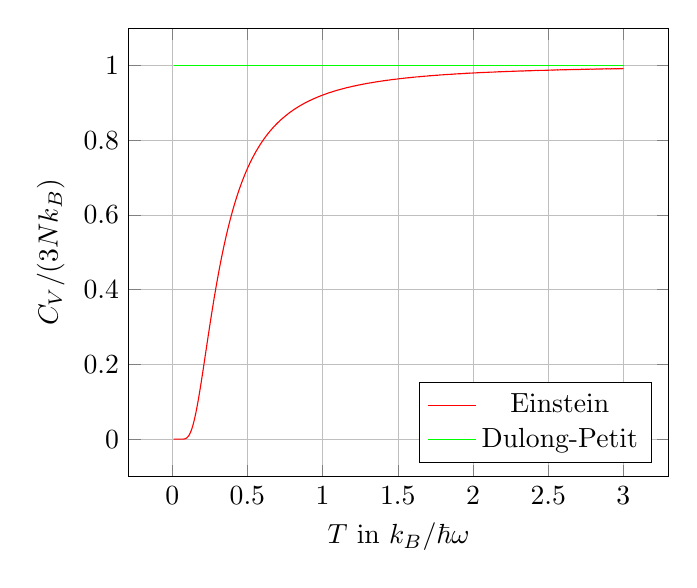
\begin{tikzpicture}
\begin{axis}[
    xlabel = $T$ in $k_B/\hbar\omega$,
    ylabel = {$C_V/(3Nk_B)$},
    legend pos=south east,
    grid=both,
    grid style={line width=.1pt, draw=gray!10},
    major grid style={line width=.2pt,draw=gray!50}]
\addplot[color=red,domain=0.01:3, samples=1000, ]{((1/(2*x))/(sinh(1/(2*x))))^2};
\addlegendentry{Einstein}
\addplot[color=green,domain=0.01:3, samples=1000, ]{1};
\addlegendentry{Dulong-Petit}
\end{axis}
\end{tikzpicture}
\end{center}

\section{Quantum Field Theory}
\subsection{{\sc Lancaster, Blundell} - Quantum Field Theory for the gifted amateur}
\subsubsection{Problem 1.1 - Snell's law via Fermat's principle}
The light travels from point $A$ in medium 1 to point $B$ in medium 2. We assume a vertical medium boundary at $x_0$ and that the light travels within a medium in the straight line. This makes $y_0$ the free parameter and the the travel time is given by
\begin{align}
    t&=\frac{s_{A0}}{c/n_1}+\frac{s_{0B}}{c/n_2}\\
    &=\sqrt{\frac{(x_A-x_0)^2+(y_A-y_0)^2}{c/n_1}}+\sqrt{\frac{(x_0-x_B)^2+(y_0-y_B)^2}{c/n_2}}
\end{align}
The local extrema of the travel time is given by
\begin{align}
    0&=\frac{dt}{dy_0}\\
    &=\frac{y_A-y_0}{s_{A0}c/n_1}+\frac{y_0-y_B}{s_{0B}c/n_2}\\
    &=\frac{\sin\alpha}{c/n_1}-\frac{\sin\beta}{c/n_2}
\end{align}
and therefore
\begin{align}
n_1\sin\alpha=n_2\sin\beta.
\end{align}

\subsection{{\sc Muenster} - Von der Quantenfeldtheorie zum Standardmodell} 
\subsubsection{Problem 2.1 - 1}
The Klein-Gordon equations is given by
\begin{align}
    \left(\partial_\mu\partial^\mu+\frac{m^2c^2}{\hbar^2}\right)\varphi&=0\\
    \left(c^2\partial_{tt}-\triangle+\frac{m^2c^2}{\hbar^2}\right)\varphi&=0
\end{align}
We make the ansatz
\begin{align}
    \varphi&=\phi_1+\phi_2\\
    \phi_1&=\frac{1}{2}\varphi-\alpha\partial_t\varphi\\
    \phi_2&=\frac{1}{2}\varphi+\alpha\partial_t\varphi
\end{align}
Then we get expressions for the time derivatives 
\begin{align}
    \phi_2-\phi_1&=2\alpha\partial_t\varphi\\
    \rightarrow\partial_t\varphi&=\frac{1}{2\alpha}(\phi_2-\phi_1)
\end{align}
and
\begin{align}
    \partial_{tt}\varphi&=c^2\left(\triangle-\frac{m^2c^2}{\hbar^2}\right)\varphi\\
    &=c^2\left(\triangle-\frac{m^2c^2}{\hbar^2}\right)(\phi_1+\phi_2)
\end{align}
Therefore we get for $\phi_{1,2}$
\begin{align}
    \partial_t\phi_1
    &=\frac{1}{2}\partial_t\varphi-\alpha\partial_{tt}\varphi\\
    &=\frac{1}{2\alpha}(\phi_2-\phi_1)-\alpha c^2\left(\triangle-\frac{m^2c^2}{\hbar^2}\right)(\phi_1+\phi_2)\\
    \partial_t\phi_2
    &=\frac{1}{2}\partial_t\varphi+\alpha\partial_{tt}\varphi\\
    &=\frac{1}{2\alpha}(\phi_2-\phi_1)+\alpha c^2\left(\triangle-\frac{m^2c^2}{\hbar^2}\right)(\phi_1+\phi_2)
\end{align}
which we can write in the form
\begin{align}
i\hbar\partial_t\begin{pmatrix}
\phi_1 \\
\phi_2 
\end{pmatrix}=-i\hbar\alpha c^2\left(\triangle-\frac{m^2c^2}{\hbar^2}\right)
\begin{pmatrix}
 1 &  1 \\
-1 & -1 
\end{pmatrix}\begin{pmatrix}
\phi_1 \\
\phi_2 
\end{pmatrix}
+\frac{i\hbar}{2\alpha}
\begin{pmatrix}
-1 &  1 \\
-1 &  1 
\end{pmatrix}
\begin{pmatrix}
\phi_1 \\
\phi_2 
\end{pmatrix}\\
=i\hbar\begin{pmatrix}
-\alpha c^2\left(\triangle-\frac{m^2c^2}{\hbar^2}\right)-\frac{1}{2\alpha} &  -\alpha c^2\left(\triangle-\frac{m^2c^2}{\hbar^2}\right)+\frac{1}{2\alpha} \\
\alpha c^2\left(\triangle-\frac{m^2c^2}{\hbar^2}\right)-\frac{1}{2\alpha} &  \alpha c^2\left(\triangle-\frac{m^2c^2}{\hbar^2}\right)+\frac{1}{2\alpha}
\end{pmatrix}
\begin{pmatrix}
\phi_1  \\
\phi_2  
\end{pmatrix}
\end{align}
Diagonalization gives
\begin{align}
    i\hbar\partial_t\phi&=\hat{H}\phi\\
    \rightarrow i\hbar\partial_tS^{-1}\phi&=\underbrace{S^{-1}\hat{H}S}_{=h}S^{-1}\phi\\
    \lambda_\pm&=\sqrt{2}mc^2\sqrt{1-\frac{\hbar^2}{m^2c^2}\triangle}
\end{align}
A semi-canonical choice for the parameter $\alpha$ is to make the $\triangle$ look like a momentum operator
\begin{align}
    \i\hbar\alpha c^2=-\frac{\hbar^2}{2m}\quad\rightarrow\quad\alpha=\frac{i\hbar}{2mc^2}
\end{align}

\subsection{{\sc Schwartz} - Quantum Field Theory and the Standard Model}

\subsubsection{Problem 2.2 Special relativity and colliders}
\begin{enumerate}
    \item Quick special relativity recap
    \begin{align}
        p'^\mu&=\Lambda^\mu_\nu p^\nu\quad p^\mu p_\mu=m^2c^2
    \end{align}
    At rest
    \begin{align}
        p^\mu p_\mu&=(p^0)^2-\vec{p}^2=(p^0)^2=m^2c^2
    \end{align}
    After Lorentz trafo in $x$ direction
    \begin{align}
        \Lambda=\begin{pmatrix}
        \gamma & -\beta\gamma & 0 & 0\\
        -\beta\gamma & \gamma & 0 & 0\\
        0 & 0 & 1 & 0\\
        0 & 0 & 0 & 1\\
        \end{pmatrix}
    \end{align}
    \begin{align}
        p'^\mu&=(\gamma p^0,-\beta\gamma p^0,0,0)\\
        &\equiv\left(\frac{E}{c},\vec{p}\right)
    \end{align}
    with $p^\mu p_\mu=m^2c^2$ we have $E^2/c^2+\vec{p}^2=m^2c^2$.
    
    Now we can solve the problem
    \begin{align}
        \frac{E_{cm}}{2}&=\sqrt{m_p^2c^4+p^2c^2}\\
        &\rightarrow p = \frac{1}{c}\sqrt{\frac{E_{cm}^2}{4}-m_p^2c^4}\equiv\beta\gamma m_pc\\
        &\rightarrow \frac{E_{cm}^2}{4}=m_p^2c^4(\beta^2\gamma^2+1)\\
        &\rightarrow \gamma=\frac{E_{cm}}{2m_pc^2}\\
        &\rightarrow\beta=\sqrt{1-\left(\frac{2m_pc}{E_{cm}}\right)^2}\approx1-\frac{1}{2}\left(\frac{2m_pc^2}{E_{cm}}\right)^2\\
        &\rightarrow c-v=2\left(\frac{m_pc^2}{E_{cm}}\right)^2c=2.69\text{m/s}
    \end{align}
    \item Using the velocity addition formula
    \begin{align}
        \Delta v=\frac{2v}{1+\frac{v^2}{c^2}}\approx c\left(1-2\left[\frac{m_pc^2}{E_{cm}}\right]^4\right)
    \end{align}
\end{enumerate}


\subsubsection{Problem 2.3 GZK bound}
\begin{enumerate}
    \item We are utilizing Plancks law
    \begin{align}
        w_\nu d\nu = \frac{8\pi h\nu^3}{c^3}\frac{d\nu}{e^{h\nu/k_BT}-1}
    \end{align}
    where the spectral energy density $w_\nu$ [J m$^{-3}$ s] gives the spacial energy density per frequency interval $d\nu$. The total radiative energy density is then given by
    \begin{align}
        \rho_\text{rad} &= \frac{8\pi h}{c^3}\int_0\infty \frac{\nu^3d\nu}{e^{h\nu/k_BT}-1}\\
        &=\frac{8\pi h}{c^3}\cdot\frac{(\pi k_B T)^4}{15h^4}\\
        &=\frac{8\pi^5k_B^4 T^4}{15h^3 c^3}=0.26\text{MeV/m}^3.
    \end{align}
    The photon density is given by
    \begin{align}
        n_\text{rad} &=\int_0^\infty\frac{w_\nu}{h\nu}d\nu\\
        &= \frac{8\pi}{c^3}\int \frac{\nu^2d\nu}{e^{h\nu/k_BT}-1}\\
        &=\frac{8\pi}{c^3}\cdot\frac{2\zeta(3) k_B^3 T^3}{h^3}\\
        &=\frac{16\pi\zeta(3) k_B^3 T^3}{h^3c^3}=416\text{cm}^{-3}.
    \end{align}
    The average photon energy is then given by
    \begin{align}
        E_\text{ph}&=\frac{\rho_\text{rad}}{n_\text{rad}}=\frac{\pi^4}{30\zeta(3)}k_BT=0.63\text{meV}\\
        \lambda_\text{ph}&=\frac{hc}{E_\text{ph}}=1.9\text{mm}
    \end{align}
    therefore it is called CM(icrowave)B.
    One obtains slightly other values if the peak of the Planck spectrum is used as definition of the average photon energy.
    \item In the center-of-mass system the total momentum before and after the collision vanishes
    \begin{align}
        \vec{p}_{p^+}^{cm}+\vec{p}_\gamma^{cm}=0=\vec{\hat{p}}_{p^+}^{cm}+\vec{\hat{p}}_{\pi^0}^{cm}.
    \end{align}
    which implies for (Lorentz-invariant) norm the systems 4-momentum $P^{cm}=p_{p^+}^{cm}+p_{\pi^0}^{cm}$
    \begin{align}
        \left(P^{cm}\right)^2&=(E_{p^+}^{cm}+E_\gamma^{cm})^2-c^2(\vec{p}_{p^+}^{cm}+\vec{p}_\gamma^{cm})^2\\
        &=(E_{p^+}^{cm}+E_\gamma^{cm})^2\\
        &=(E^{cm})^2\\
        &\overset{!}{=}(E_{p^+}+E_\gamma)^2-c^2(\vec{p}_{p^+}+\vec{p}_\gamma)^2\\
        &\overset{!}{=}(\hat{E}_{p^+}+\hat{E}_{\pi^0})^2-c^2(\vec{\hat{p}}_{p^+}+\vec{\hat{p}}_{\pi^0})^2
    \end{align}
    with $p^i=\hbar k^i=\hbar(\omega,\vec{k})=\hbar(\omega,\frac{2\pi}{\lambda}\vec{e}_k)=h(\nu,\frac{\nu}{c}\vec{e}_k)$ and the values before
    \begin{align}
        E_{p^+}&=m_{p^+}c^2+T_{p^+}\\
        E_\gamma&=h\nu\\  
        (\vec{p}_{p^+})^2
        &=\frac{1}{c^2}\left[(E_{p^+})^2-(m_{p^+})^2c^4\right]\\
        &=\frac{T_{p^+}}{c^2}\left[T_{p^+}+2m_{p^+}c^2\right]\\
        (\vec{p}_\gamma)^2&=\frac{h^2\nu^2}{c^2}
    \end{align}
    At the threshold the $\pi^0$ is created without any kinetic energy. As the total momentum is vanishing the proton
    also needs to be at rest
    \begin{align}
        (E_{p^+}+E_\gamma)^2-c^2(\vec{p}_{p^+}+\vec{p}_\gamma)^2&=\left(m_{p^+}c^2+m_{\pi^0}c^2\right)^2\\
        E_{p^+}^2+2E_{p^+}E_\gamma+E_\gamma^2-c^2\left(\vec{p}_{p^+}^2+\vec{p}_\gamma^2-2\vec{p}_{p^+}\cdot\vec{p}_\gamma\right)&=\left(m_{p^+}c^2+m_{\pi^0}c^2\right)^2\\
        m_{p^+}^2c^4+2E_{p^+}E_\gamma+2c^2\vec{p}_{p^+}\cdot\vec{p}_\gamma&=\left(m_{p^+}c^2+m_{\pi^0}c^2\right)^2\\
        m_{p^+}^2c^4+2E_{p^+}E_\gamma+2E_\gamma\sqrt{E_{p^+}^2-m_{p^+}^2c^2}\cos{\phi}&=\left(m_{p^+}c^2+m_{\pi^0}c^2\right)^2\\
        E_{p^+}E_\gamma+E_\gamma\sqrt{E_{p^+}^2-m_{p^+}^2c^2}\cos{\phi}&=\left(m_{p^+}+\frac{m_{\pi^0}}{2}\right)m_{\pi^0}c^4
    \end{align}
    Now we can square the equation and solve approximately assuming $E_\gamma\ll m_{p^+}c^2$
    \begin{align}
        E_\gamma\sqrt{E_{p^+}^2-m_{p^+}^2c^2}\cos{\phi}&=\left(m_{p^+}+\frac{m_{\pi^0}}{2}\right)m_{\pi^0}c^4-E_{p^+}E_\gamma\\
        E_\gamma^2\left(E_{p^+}^2-m_{p^+}^2c^2\right)\cos^2{\phi}
        &=\left(m_{p^+}+\frac{m_{\pi^0}}{2}\right)^2m_{\pi^0}^2c^8+(E_{p^+}E_\gamma)^2-2E_{p^+}E_\gamma\left(m_{p^+}+\frac{m_{\pi^0}}{2}\right)m_{\pi^0}c^4\\
        -E_\gamma^2m_{p^+}^2c^2\cos^2{\phi}
        &=\left(m_{p^+}+\frac{m_{\pi^0}}{2}\right)^2m_{\pi^0}^2c^8-2E_{p^+}E_\gamma\left(m_{p^+}+\frac{m_{\pi^0}}{2}\right)m_{\pi^0}c^4\\
        E_{p^+}&\approx\frac{\left(m_{p^+}+m_{\pi^0}/2\right)m_{\pi^0}c^4}{2E_\gamma}\\
        &=10.8\cdot 10^{19}\text{eV}
    \end{align}
    \item By assumption the $p^+$ and the $\pi^0$ would rest in the CM system
    \begin{align}
        (P^\mu)^{cm}&=(p^\mu_{p^+})^{cm}+(p^\mu_{\pi^0})^{cm}\\
                    &=\left([m_{p^+}+m_{\pi^0}]c^2,\vec{0}\right)\\
                    &=\Lambda^\mu_\alpha\left[\hat p^\alpha_{p^+}+\hat p^\alpha_{\pi^0}\right]\\
                    &=\Lambda^\mu_\alpha\left[ p^\alpha_{p^+}+ p^\alpha_{\gamma}\right]\\
    \end{align}
    We can therefore calculate $\gamma$
    \begin{align}
        \mu=1:\quad0&=\underbrace{\Lambda^1_0}_{-\gamma\beta}(E_{p^+}+E_\gamma)+\underbrace{\Lambda^1_1}_{\gamma}c(p^x_{p^+}+p^x_\gamma)\\
        &=-\gamma\beta(E_{p^+}+E_\gamma)+\gamma\left(\sqrt{E_{p^+}^2-m_p^2c^4}+E_\gamma\right)\\
        &\rightarrow\beta=\frac{\sqrt{E_{p^+}^2-m_p^2c^4}+E_\gamma}{E_{p^+}+E_\gamma}\approx\frac{\sqrt{E_{p^+}^2-m_p^2c^4}}{E_{p^+}}\\
        &\rightarrow\gamma=\frac{1}{\sqrt{1-\beta^2}}=\frac{E_{p^+}}{m_{p^+}c^2}
    \end{align}
    which can be used to calculate the pion momentum
    \begin{align}
        c\hat{p}_{\pi^0}&=\Lambda^0_\mu (p_{\pi^0}^\mu)^{cm}\\
        &=\Lambda^0_0 (p_{\pi^0}^0)^{cm}\\
        &=\gamma m_{\pi^0}c^2\\
        &=E_{p^+}\frac{m_{\pi^0}}{m_{p^+}}.
    \end{align}
    The $p+$ energy after the collision is then given by 
    \begin{align}
        E_{p^+}+E_\gamma&=\hat E_{p^+}+\hat E_{\pi^0}\\
        \rightarrow\hat E_{p^+}&=E_{p^+}+E_\gamma - \hat E_{\pi^0}\\
        &=E_{p^+}+E_\gamma - \sqrt{m_{\pi^0}^2c^4+\hat{\vec{p}}_{\pi^0}c^2}\\
        &=E_{p^+}+E_\gamma - \sqrt{m_{\pi^0}^2c^4+E_{p^+}^2\frac{m_{\pi^0}^2}{m_{p^+}^2}}\\
        &=E_{p^+}+E_\gamma - m_{\pi^0}c^2\sqrt{1+\frac{E_{p^+}^2}{m_{p^+}^2c^4}}\\
        &\approx E_{p^+} - m_{\pi^0}c^2\frac{E_{p^+}}{m_{p^+}c^2}\\
        &=E_{p^+}\left(1-\frac{m_{\pi^0}}{m_{p^+}}\right)\\
        &\approx0.85\cdot E_{p^+}.
    \end{align}
\end{enumerate}

\subsubsection{Problem 2.5 Compton scattering}
\begin{enumerate}
    \item the binding energy of outer(!!!) electrons is in the eV range while typical X-rays energies are in the keV range.
    \item In the nonrelativistic case we have energy and momentum conservation
    \begin{align}
        \frac{hc}{\lambda}&=\frac{hc}{\lambda'}+\frac{1}{2}m_ev^2\\
        \frac{h}{\lambda}&=\frac{h}{\lambda'}\cos\theta+m_ev\cos\phi\\
        0&=\frac{h}{\lambda'}\sin\theta+m_ev\sin\phi
    \end{align}
    then we see
    \begin{align}
        v=\sqrt{\frac{2hc}{m_e}\left(\frac{1}{\lambda}-\frac{1}{\lambda'}\right)}
        =\sqrt{\frac{2hc}{m_e}\frac{\lambda'-\lambda}{\lambda\lambda'}}
    \end{align}
    and
    \begin{align}
        \sin\phi&=-\frac{h}{m_ev}\frac{1}{\lambda'}\sin\theta\\
        \cos\phi&=\frac{h}{m_ev}\frac{1}{\lambda'}\left(\frac{\lambda'}{\lambda}-\cos\theta\right)\\
        \rightarrow1&=\sin^2\phi+\cos^2\phi\\
        &=\frac{h^2}{m_e^2v^2\lambda'^2}\left(\sin^2\theta+\frac{\lambda'^2}{\lambda^2}-2\frac{\lambda'}{\lambda}\cos\theta+\cos^2\theta\right)\\
        &=\frac{h^2}{m_e^2v^2\lambda'^2}\left(1+\frac{\lambda'^2}{\lambda^2}-2\frac{\lambda'}{\lambda}\cos\theta\right)\\
        &=\frac{h\lambda}{2m_ec\lambda'(\lambda'-\lambda)}\left(1+\frac{\lambda'^2}{\lambda^2}-2\frac{\lambda'}{\lambda}\cos\theta\right)\\
        &=\frac{h}{2m_ec(\lambda'-\lambda)}\left(\frac{\lambda}{\lambda'}+\frac{\lambda'}{\lambda}-2\cos\theta\right)\\
        \lambda'-\lambda&\approx\frac{h}{m_ec}\left(1-\cos\theta\right)
    \end{align}
    where we used $\lambda\approx\lambda'$.
    \item 
\end{enumerate}
    
\subsubsection{Problem 2.6 Lorentz invariance}
\begin{enumerate}
    \item With $\omega_k=\sqrt{\vec{k}^2+m^2}$
    \begin{align}
        \int_{-\infty}^\infty dk^0\delta(k^2-m^2)\theta(k^0)
        &=\int_{-\infty}^\infty dk^0\delta({k^0}^2-[\vec{k}^2+m^2])\theta(k^0)\\
        &=\frac{\theta(\omega_k)}{2\omega_k}+\frac{\theta(-\omega_k)}{2\omega_k}\\
        &=\frac{1}{2\omega_k}
    \end{align}
    \item Under Lorentz transformations we have $k^2-m^2=0$. For orthochronous transformation we have $k^0 ...$
    \item Now we can put it all together
    \begin{align}
        \int d^4k\delta(k^2-m^2)\theta(k^0)
        &=\int d^3k\int dk^0\delta(k^2-m^2)\theta(k^0)\\
        &=\int\frac{d^3k}{2\omega_k}
    \end{align}
\end{enumerate}

\subsubsection{Problem 2.7 Coherent states}
\begin{enumerate}
\item 
\begin{align}
    \partial_z\left(e^{-za^\dagger} a e^{-za^\dagger}\right)
    &=-e^{-za^\dagger}a^\dagger a e^{-za^\dagger}+e^{-za^\dagger} a a^\dagger e^{-za^\dagger}\\
    &=e^{-za^\dagger} [a,a^\dagger] e^{-za^\dagger}\\
    &=1
\end{align}
\item Rolling the $a$ through the $(a^\dagger)^k$ using the commutator $[a,a^\dagger]=1$
\begin{align}
    a|z\rangle
    &=a e^{za^\dagger}|0\rangle\\
    &=a\sum_{k=0}\frac{1}{k!}z^k(a^\dagger)^k|0\rangle\\
    &=a|0\rangle+\sum_{k=1}\frac{k}{k!}z^k(a^\dagger)^{k-1}|0\rangle\\
    &=z\sum_{n=0}\frac{1}{n!}z^n(a^\dagger)^{n}|0\rangle\\
    &=z|z\rangle
\end{align}
\item With $a^\dagger|n\rangle=\sqrt{n+1}|n+1\rangle$ and using the $|z\rangle$ is an eigenstate of $a$ we have
\begin{align}
    \langle n|z\rangle&=\frac{1}{\sqrt{n!}}\langle0|a^n|z\rangle
    =\frac{z^n}{\sqrt{n!}}\langle0|z\rangle
    =\frac{z^n}{\sqrt{n!}}\langle0|e^{za^\dagger}|0\rangle\\
    &=\frac{z^n}{\sqrt{n!}}\langle0|1+za^\dagger+\frac{1}{2}z^2(a^\dagger)^2+...|0\rangle\\
    &=\frac{z^n}{\sqrt{n!}}\langle0|0\rangle
    =\frac{z^n}{\sqrt{n!}}
\end{align}
where we used $\langle0|a^\dagger=0$.
\item With
\begin{align}
    a+a^\dagger&=\sqrt{\frac{m\omega}{2}}2q\quad\rightarrow\quad q=\frac{1}{\sqrt{2m\omega}}(a+a^\dagger)\\
    a-a^\dagger&=\sqrt{\frac{m\omega}{2}}2\frac{ip}{m\omega}\quad\rightarrow\quad p=-i\frac{\sqrt{m\omega}}{\sqrt{2}}(a-a^\dagger)
\end{align}
and $a|z\rangle=z|z\rangle$ and $\langle z|a^\dagger=\bar{z}\langle z|$ 
\begin{align}
    \langle z|q|z\rangle
    &=\frac{1}{\sqrt{2m\omega}}\langle z|a+a^\dagger|z\rangle
    =\frac{1}{\sqrt{2m\omega}}\langle z|z\rangle(z+\bar{z})\\
    \langle z|p|z\rangle&=-i\frac{\sqrt{m\omega}}{\sqrt{2}}\langle z|a-a^\dagger|z\rangle=
    -i\frac{\sqrt{m\omega}}{\sqrt{2}}\langle z|z\rangle(z-\bar{z})\\
    \langle z|q^2|z\rangle
    &=\frac{1}{2m\omega}\langle z|aa+\underbrace{aa^\dagger}_{=1+a^\dagger a}+a^\dagger a+a^\dagger a^\dagger|z\rangle\\
    &=\frac{1}{2m\omega}\langle z|z\rangle\left(z^2+1+2z\bar{z}+\bar{z}^2\right)\\
    \langle z|p^2|z\rangle
    &=-\frac{m\omega}{2}\langle z|aa-\underbrace{aa^\dagger}_{=1+a^\dagger a}-a^\dagger a+a^\dagger a^\dagger|z\rangle\\
    &=-\frac{m\omega}{2}\langle z|z\rangle\left(z^2-1-2z\bar{z}+\bar{z}^2\right)
\end{align}
Therefore
\begin{align}
    \Delta q^2
    &=\langle q^2\rangle-\langle q\rangle^2\\
    &=\frac{1}{2m\omega}\left(z^2+1+2z\bar{z}+\bar{z}^2\right)-\left(\frac{1}{\sqrt{2m\omega}}(z+\bar{z})\right)^2\\
    &=\frac{1}{2m\omega}
\end{align}
and
\begin{align}
    \Delta p^2
    &=\langle p^2\rangle-\langle p\rangle^2\\
    &=-\frac{m\omega}{2}\left(z^2-1-2z\bar{z}+\bar{z}^2\right)-\left(-i\frac{\sqrt{m\omega}}{\sqrt{2}}(z-\bar{z})\right)^2\\
    &=\frac{m\omega}{2}
\end{align}
which means
\begin{align}
    \Delta p\Delta q=\frac{1}{\sqrt{2m\omega}}\frac{\sqrt{m\omega}}{\sqrt{2}}=\frac{1}{2}.
\end{align}
\item At first let's construct the eigenstate $|w\rangle$ for $a$ manually
\begin{align}
    a|w\rangle=c_w|w\rangle
\end{align}
Expanding the eigenstate with $a^\dagger|n\rangle=\sqrt{n+1}|n+1\rangle$
\begin{align}
    |w\rangle
    &=\sum_n\alpha_n|n\rangle\\
    a|w\rangle
    &=\sum_n\alpha_n\sqrt{n}|n-1\rangle\overset{!}{=}c_w\sum_n\alpha_n|n\rangle=c_w|n\rangle\\
    &\rightarrow\alpha_n\sqrt{n}=c_w\alpha_{n-1}\\
    &\rightarrow\alpha_n=\frac{c_w}{\sqrt{n}}\alpha_{n-1}\\
    |w\rangle
    &=\sum_n\alpha_0\frac{c_w^n}{\sqrt{n!}}|n\rangle
    =\alpha_0\sum_n\frac{c_w^n}{n!}(a^\dagger)^n|0\rangle
    =\alpha_0 e^{c_wa^\dagger}|0\rangle
\end{align}
Now we do the same for $a^\dagger$
\begin{align}
    a^\dagger|v\rangle=c_v|v\rangle
\end{align}
Expanding the eigenstate 
\begin{align}
    |v\rangle
    &=\sum_n\beta_n|n\rangle\\
    a^\dagger|v\rangle
    &=\sum_n\beta_n\sqrt{n+1}|n+1\rangle\overset{!}{=}c_v\sum_n\beta_n|n\rangle=c_v|n\rangle\\
    &\rightarrow\beta_{n}\sqrt{n+1}=c_v\beta_{n+1}\\
    &\rightarrow\beta_{n+1}=\frac{\sqrt{n+1}}{c_v}\beta_{n}\\
    |v\rangle
    &=\sum_n\beta_0\frac{\sqrt{n!}}{c_v^n}|n\rangle=\beta_0\sum_n\frac{1}{c_v^n}(a^\dagger)^n|0\rangle
\end{align}
Now we calculate with $\langle 0|a^\dagger=0$
\begin{align}
    \langle 0|a^\dagger|v\rangle&=\beta_0\sum_n\frac{1}{c_v^n}\langle 0|(a^\dagger)^{n+1}|0\rangle\\
    &=\beta_0\frac{1}{c_v^0}\langle 0|a^\dagger|0\rangle\\
\end{align}
\end{enumerate}

\subsubsection{Problem 3.5 Spontaneous symmetry}
\begin{enumerate}
    \item 
    \begin{align}
    \mathscr{L}=-\frac{1}{2}\phi\Box\phi+\frac{1}{2}m^2\phi^2-\frac{\lambda}{4!}\phi^4\\
    \frac{\partial\mathscr{L}}{\partial \phi}-\partial_\beta\frac{\partial\mathscr{L}}{\partial(\partial_\beta \phi)}=0\\
    \rightarrow -\frac{1}{2}\Box\phi+m^2\phi-\frac{\lambda}{3!}\phi^3=0
\end{align}
\end{enumerate}

\subsubsection{Problem 3.1 Higher order Lagrangian}
With the principle of least action
\begin{align}
\delta S=\delta\int\mathcal{L}d^4x=\int\delta\mathcal{L}d^4x
\end{align}
we calculate
\begin{align}
\delta\mathcal{L}
&=\frac{\partial \mathcal{L}}{\partial\phi}\delta\phi+
\frac{\partial \mathcal{L}}{\partial(\partial_\mu\phi)}\delta(\partial_\mu\phi)+
\frac{\partial \mathcal{L}}{\partial(\partial_\nu\partial_\mu\phi)}\delta(\partial_nu\partial_\mu\phi)+...
\end{align}
Now we can integrate each term
\begin{align}
\delta\mathcal{L}_0&=\int \frac{\partial \mathcal{L}}{\partial\phi}\delta\phi d^4x\\
%
\delta\mathcal{L}_1&=\int \frac{\partial \mathcal{L}}{\partial(\partial_\mu\phi)}\delta(\partial_\mu\phi) d^4x
=\int \frac{\partial \mathcal{L}}{\partial(\partial_\mu\phi)}\partial_\mu\delta\phi d^4x\\
&=\left.\frac{\partial \mathcal{L}}{\partial(\partial_\mu\phi)}\delta\phi\right|_{\partial\Omega}-\int \partial_\mu\frac{\partial \mathcal{L}}{\partial(\partial_\mu\phi)}\delta\phi d^4x\\
%
\delta\mathcal{L}_2&=\int \frac{\partial \mathcal{L}}{\partial(\partial_\nu\partial_\mu\phi)}\delta(\partial_\nu\partial_\mu\phi) d^4x
=\int \frac{\partial \mathcal{L}}{\partial(\partial_\nu\partial_\mu\phi)}\partial_\nu\delta\partial_\mu\phi d^4x\\
&=\left.\frac{\partial \mathcal{L}}{\partial(\partial_\nu\partial_\mu\phi)}\delta\partial_\mu\phi\right|_{\partial\Omega}-\int \partial_\nu\frac{\partial \mathcal{L}}{\partial(\partial_\nu\partial_\mu\phi)}\delta\partial_\mu\phi d^4x\\
&=\left.\frac{\partial \mathcal{L}}{\partial(\partial_\nu\partial_\mu\phi)}\delta\partial_\mu\phi\right|_{\partial\Omega}-\left.\partial_\nu\frac{\partial \mathcal{L}}{\partial(\partial_\nu\partial_\mu\phi)}\delta\phi\right|_{\partial\Omega}+\int \partial_\mu\partial_\nu\frac{\partial \mathcal{L}}{\partial(\partial_\nu\partial_\mu\phi)}\delta\phi d^4x
\end{align}
Requiring that all derivatives vanish at infinity we obtain
\begin{align}
\delta S=\int d^4x\left(
\frac{\partial \mathcal{L}}{\partial\phi}
- \partial_\mu\frac{\partial \mathcal{L}}{\partial(\partial_\mu\phi)}
+\partial_\mu\partial_\nu\frac{\partial \mathcal{L}}{\partial(\partial_\nu\partial_\mu\phi)}-...
\right)\delta\phi
\end{align}
and therefore
\begin{align}
\frac{\partial \mathcal{L}}{\partial\phi}
- \partial_\mu\frac{\partial \mathcal{L}}{\partial(\partial_\mu\phi)}
+\partial_\mu\partial_\nu\frac{\partial \mathcal{L}}{\partial(\partial_\nu\partial_\mu\phi)}-...=0
\end{align}

\subsubsection{Problem 3.6 Yukawa potential}
\begin{enumerate}
\item We slit the Lagranian in three parts
\begin{align}
\mathscr{L}&=-\frac{1}{4}F_{\mu\nu}^2+\frac{1}{2}m^2A_\mu^2-A_\mu J_\mu\\
&=\mathscr{L}_F+\mathscr{L}_m+\mathscr{L}_J
\end{align}
with the Euler Lagrange equations
\begin{align}
        \frac{\partial\mathscr{L}}{\partial A_\alpha}-\partial_\beta\frac{\partial\mathscr{L}}{\partial(\partial_\beta A_\alpha)}=0
\end{align}
with
\begin{align}
    \frac{\partial(\partial_\mu A_\nu)}{\partial(\partial_\beta A_\alpha)}=\delta_{\mu\beta}\delta_{\nu\alpha}
\end{align}
we can calculate
\begin{align}
    \frac{\partial\mathscr{L}_m}{\partial A_\alpha}-\partial_\beta\frac{\partial\mathscr{L}_m}{\partial(\partial_\beta A_\alpha)}&=m^2A_\alpha\\
    \frac{\partial\mathscr{L}_J}{\partial A_\alpha}-\partial_\beta\frac{\partial\mathscr{L}_J}{\partial(\partial_\beta A_\alpha)}&=-J_\alpha\\
    \frac{\partial\mathscr{L}_F}{\partial A_\alpha}-\partial_\beta\frac{\partial\mathscr{L}_F}{\partial(\partial_\beta A_\alpha)}&=-\frac{1}{4}\partial_\beta\left(-2F_{\mu\nu}(\delta_{\mu\beta}\delta_{\nu\alpha}-\delta_{\nu\beta}\delta_{\mu\alpha})\right)\\
    &=\frac{1}{4}\partial_\beta\left(2(F_{\beta\alpha}-F_{\alpha\beta})\right)\\
    &=\partial_\beta F_{\beta\alpha}\\
    &=\partial_\beta\partial_\beta A_\alpha-\partial_\beta\partial_\alpha A_\beta
\end{align}
to obtain (the Proca equation)
\begin{align}
    \Box A_\alpha-\partial_\beta\partial_\alpha A_\beta+m^2A_\alpha-J_\alpha=0.
\end{align}
Now we can calculate the divergence of the equations
\begin{align}
    \partial_\alpha\left(\Box A_\alpha-\partial_\beta\partial_\alpha A_\beta+m^2A_\alpha-J_\alpha\right)=0.\\
    \Box \partial_\alpha A_\alpha-\partial_\alpha\partial_\alpha\partial_\beta A_\beta+m^2\partial_\alpha A_\alpha-\underbrace{\partial_\alpha J_\alpha}_{=0}=0
\end{align}
which implies $\partial_\alpha A_\alpha=0$ and therefore
\begin{align}
    \Box A_\alpha+m^2A_\alpha-J_\alpha=0.
\end{align}
\item For $A_0$ we have for a static potential
\begin{align}
    (\partial_{tt}-\triangle)A_0+m^2A_0-e\delta(x)=0\\
    -\triangle A_0+m^2A_0-e\delta(x)=0.
\end{align}
A Fourier transformation of the equation of motion yields
\begin{align}
    -(ik)^2 A_0(k)+m^2A_0(k)-e=0\\
    \rightarrow A_0(k)=\frac{e}{k^2+m^2}
\end{align}
which we can now transform back 
\begin{align}
    A_0
    &=\frac{e}{(2\pi)^3}\int d^3k\frac{e^{ikx}}{k^2+m^2}\\
    &=\frac{e}{4\pi r} e^{-mr}
\end{align}
where we used the integral evaluation from {\sc Kachelriess} Problem 3.5.
\item 
\begin{align}
    \lim_{m\rightarrow0}\frac{e}{4\pi r} e^{-mr}=\frac{e}{4\pi r}
\end{align}
\item Scaling down the Coulomb potential exponentially with a characteristic length of $1/m$.
\item We can expand and the integrate each term by parts to move over the partial derivatives 
\begin{align}
    \mathscr{L}_F
    &=-\frac{1}{4}F_{\mu\nu}^2\\
    &=-\frac{1}{4}(\partial_\mu A_\nu-\partial_\nu A_\mu)(\partial_\nu A_\mu-\partial_\mu A_\nu)\\
    &=-\frac{1}{4}\left(\partial_\mu A_\nu \partial_\nu A_\mu-\partial_\mu A_\nu \partial_\mu A_\nu
        -\partial_\nu A_\mu \partial_\nu A_\mu + \partial_\nu A_\mu\partial_\mu A_\nu\right)\\
    &=-\frac{1}{4}\left(- A_\nu \partial_\nu \partial_\mu A_\mu+ A_\nu \partial_\mu\partial_\mu A_\nu
        + A_\mu \partial_\nu\partial_\nu A_\mu -  A_\mu\partial_\mu \partial_\nu A_\nu\right)\\
    &=\frac{1}{2}\left( A_\nu \partial_\nu \underbrace{\partial_\mu A_\mu}_{=0}- A_\nu \Box A_\nu\right)\\ 
    &=-\frac{1}{2}A_\nu \Box A_\nu
\end{align}
We can plug this into the full Lagrangian (renaming the summation index)
\begin{align}
    \mathscr{L}&=-\frac{1}{2}A_\mu \Box A_\mu+\frac{1}{2}m^2A_\mu^2-A_\mu J_\mu\\
    &=\frac{1}{2}A_\mu\left(-\Box+m^2 \right)A_\mu-A_\mu J_\mu\\
\end{align}    
\end{enumerate}

\subsubsection{Problem 3.7 Perihelion shift of Mercury by dimensional analysis}
\begin{enumerate}[label=(\alph*)]
\item Lets summarize the rules of dimensional analysis 

\begin{center}
\begin{tabular}{ lccc } 
 \hline
 varible & SI unit &equation & natural unit \\ 
 \hline\hline
 $c$               & m/s    & -                        & 1        \\
 $\hbar$           & Js     & -                        & 1        \\
 Velocity          & m/s    & -                        & 1      \\
 mass              & kg     & $E=mc^2$                 & $E$      \\
 frequency         & 1/s    & $E=\hbar\omega$          & $E$      \\
 time              & s      & $t=2\pi/\omega$          & $E^{-1}$ \\
 length            & m      & $s=ct$                   & $E^{-1}$ \\
 $\partial_\mu$    & 1/m    & -                        & $E$      \\
 momentum          & kg\,m/s& $E=p^2/2m$               & $E$      \\
 action            & Js     & $S=Et$                   & 1        \\
 $\mathcal{L}$     & J/m$^3$& $S=\int d^4x\mathcal{L}$ & $E^4$    \\
 energy density    & J/m$^3$& $\rho=E/V$               & $E^4$    \\
 $T^{\mu\nu}$      & J/m$^3$& $\rho=E/V$               & $E^4$    \\
 \hline
\end{tabular}
\end{center}
Now we can do a dimensions count for each term
\begin{align}
\underbrace{\mathcal{L}}_{=4}&=-\frac{1}{2}\underbrace{h\Box h}_{2\cdot[h]+2}+ \underbrace{M_\text{Pl}^a h^2\Box h}_{=a+3\cdot[h]+2}-\underbrace{M_\text{Pl}^bhT}_{b+[h]+4}\\
&\rightarrow\quad[h]=1\\
&\rightarrow\quad a=-1\\
&\rightarrow\quad b=-1
\end{align} 
\item Deriving the equations of motions
\begin{align}
\mathcal{L}&=-\frac{1}{2}h\Box h+\frac{1}{M_\text{Pl}}h^2\Box h-\frac{1}{M_\text{Pl}}hT\\
\frac{\partial\mathcal{L}}{\partial h}&=-\frac{1}{2}\cdot2\cdot\Box h+2\frac{1}{M_\text{Pl}}h\Box h-\frac{1}{M_\text{Pl}}T\\
\frac{\partial\mathcal{L}}{\partial(\partial h)}&=0\\
&\rightarrow\Box h=\frac{4}{M_\text{Pl}}h\Box h-\frac{2}{M_\text{Pl}}T
\end{align}
which is not the given result. But
alternatively we can integrate the Lagrangian by parts (neglecting the boundary terms) and get
\begin{align}
\mathcal{L}&=\frac{1}{2}\partial h\partial h-\frac{1}{M_\text{Pl}}\partial(h^2)\partial h-\frac{1}{M_\text{Pl}}hT\\
\frac{\partial\mathcal{L}}{\partial h}&=-\frac{1}{M_\text{Pl}}T\\
\frac{\partial\mathcal{L}}{\partial(\partial h)}&=\Box h-\frac{1}{M_\text{Pl}}\Box(h^2)\\
&\rightarrow\Box h=\frac{1}{M_\text{Pl}}\Box(h^2)-\frac{1}{M_\text{Pl}}T
\end{align}
\item 
\item 
\item 
\item 
\item 
\end{enumerate}



\subsection{{\sc Srednicki} - Quantum Field Theory}
\subsubsection{Problem 1.2 - Schroedinger equation}
\begin{align}
    H&=\int d^3x a^\dagger(x)\left(-\frac{\hbar^2}{2m}\triangle_x+V(x)\right)a(x)+\frac{1}{2}\int d^3xd^3yV(x-y)a^\dagger(x)a^\dagger(y)a(x)a(y)\\
    |\psi,t\rangle&=\int d^3x_1...d^3x_n\psi(x_1,...,x_n;t)a^\dagger(x_1)...a^\dagger(x_n)|0\rangle
\end{align}
\begin{enumerate}
    \item Bosons:
    With the commutations relation and $a|0\rangle=0$
    \begin{align}
        a(x)a^\dagger(x_1)...a^\dagger(x_n)|0\rangle
        &=\left(\delta^3(x-x_1)-a^\dagger(x_1)a(x)\right)...a^\dagger(x_n)|0\rangle\\
        &=\sum_{k=1}^n(-1)^{k-1} \delta^3(x-x_k)\underbrace{a^\dagger(x_1)...a^\dagger(x_n)}_{(n-1) \times a^\dagger}|0\rangle
    \end{align}
    and similar
    \begin{align}
        a(y)a(x)a^\dagger(x_1)...a^\dagger(x_n)|0\rangle
        &=\sum_{j\neq k}^n \delta^3(x-x_k)\delta^3(y-x_j)\underbrace{a^\dagger(x_1)...a^\dagger(x_n)}_{(n-2) \times a^\dagger}|0\rangle
    \end{align}
    we obtain
	\begin{align}
		i\hbar\frac{\partial}{\partial t}|\psi,t\rangle
		&=\int d^3x_1...d^3x_n\frac{\partial}{\partial t}\psi(x_1,...,x_n;t)a^\dagger(x_1)...a^\dagger(x_n)|0\rangle 
	\end{align}
    and
    \begin{align}
        H|\psi,t\rangle=&\sum_{k=1}^na^\dagger(x_k)\left(-\frac{\hbar^2}{2m}\triangle_{x_k}+V(x_k)\right)\psi(x_1,...,x_n;t)\underbrace{a^\dagger(x_1)...a^\dagger(x_n)}_{(n-1) \times a^\dagger}|0\rangle\\
        &+\frac{1}{2}\sum_{j\neq k}^nV(x_k-x_j)\psi(x_1,...,x_n;t)a^\dagger(x_k)a^\dagger(x_j)\underbrace{a^\dagger(x_1)...a^\dagger(x_n)}_{(n-2) \times a^\dagger}|0\rangle
    \end{align}
    \item Fermions:
\end{enumerate}

\subsubsection{Problem 2.1 - Infinitesimal LT}
\begin{align}
g_{\mu\nu}\Lambda^\mu_{\;\rho}\Lambda^\nu_{\;\sigma}&=g_{\rho\sigma}\\
g_{\mu\nu}\left(\delta^\mu_{\;\rho}+\delta\omega^\mu_{\;\rho}\right)\left(\delta^\nu_{\;\sigma}+\delta\omega^\nu_{\;\sigma}\right)&=g_{\rho\sigma}\\
g_{\mu\nu}\left(\delta^\mu_{\;\rho}\delta^\nu_{\;\sigma}+\delta^\nu_{\;\sigma}\cdot\delta\omega^\mu_{\;\rho}+\delta^\mu_{\;\rho}\cdot\delta\omega^\nu_{\;\sigma}+\mathcal{O}(\delta\omega^2)\right)&=g_{\rho\sigma}\\
g_{\rho\sigma}+g_{\mu\sigma}\cdot\delta\omega^\mu_{\;\rho}+g_{\rho\nu}\cdot\delta\omega^\nu_{\;\sigma}&=g_{\rho\sigma}
\end{align}
which implies
\begin{align}
\delta\omega_{\sigma\rho}+\delta\omega_{\rho\sigma}=0
\end{align}

\subsubsection{Problem 2.2 - Infinitesimal LT II}
Important: each $M^{\mu\nu}$ is an operator and $\delta\omega$ is just a coefficient matrix so $\delta\omega _{\mu\nu}M^{\mu\nu}$ ist a weighted sum of operators.
\begin{align}
U(\Lambda^{-1}\Lambda'\Lambda)&=U(\Lambda^{-1})U(\Lambda')U(\Lambda)\\
U(\Lambda^{-1}(I+\delta\omega')\Lambda)&=U(\Lambda^{-1})\left(I+\frac{i}{2\hbar}\delta\omega'_{\mu\nu}M^{\mu\nu}\right)U(\Lambda)\\
U(I+\Lambda^{-1}\delta\omega'\Lambda)&=I+\frac{i}{2\hbar}\delta\omega'_{\mu\nu}U(\Lambda^{-1})M^{\mu\nu}U(\Lambda)
\end{align}
now we calculate recalling successive LT's $(\Lambda^{-1})^{\varepsilon}_{\;\gamma}\delta\omega'^\gamma_{\;\;\beta}\Lambda^\beta_{\;\alpha}x^\alpha$
\begin{align}
(\Lambda^{-1}\delta\omega'\Lambda)_{\rho\sigma}
&=g_{\varepsilon\rho}(\Lambda^{-1})^{\varepsilon}_{\;\mu}\delta\omega'^\mu_{\;\;\nu}\Lambda^\nu_{\;\sigma}\\
&=g_{\varepsilon\rho}\Lambda^{\;\varepsilon}_{\mu}\delta\omega'^\mu_{\;\;\nu}\Lambda^\nu_{\;\sigma}\\
&=\delta\omega'_{\mu\nu}\Lambda^{\mu}_{\;\rho}\Lambda^\nu_{\;\sigma}
\end{align}
now we can rewrite $U(I+\Lambda^{-1}\delta\omega'\Lambda)$ and therefore
\begin{align}
\delta\omega'_{\mu\nu}\Lambda^{\mu}_{\;\rho}\Lambda^\nu_{\;\sigma}M^{\rho\sigma}&=\delta\omega'_{\mu\nu}U(\Lambda^{-1})M^{\mu\nu}U(\Lambda)
\end{align}
As all $\delta\omega'$ components are basically independent the equation must hold for each pair $\mu,\nu$.

\subsubsection{Problem 2.3 - Commutator of LT generators}
LHS:
\begin{align}
U(\Lambda^{-1})M^{\mu\nu}U(\Lambda)
&\simeq\left(I-\frac{i}{2\hbar}\delta\omega_{\alpha\beta}M^{\alpha\beta}\right)M^{\mu\nu}\left(I+\frac{i}{2\hbar}\delta\omega_{\rho\sigma}M^{\rho\sigma}\right)\\
&\simeq M^{\mu\nu}-\frac{i}{2\hbar}\delta\omega_{\rho\sigma}(M^{\rho\sigma}M^{\mu\nu}-M^{\mu\nu}M^{\rho\sigma})+\mathcal{O}(\delta\omega^2)\\
&\simeq M^{\mu\nu}-\frac{i}{2\hbar}\delta\omega_{\rho\sigma}[M^{\rho\sigma},M^{\mu\nu}]
\end{align}
RHS:
\begin{align}
\Lambda^{\mu}_{\;\rho}\Lambda^\nu_{\;\sigma}M^{\rho\sigma}
&\simeq\left(\delta^{\mu}_{\;\rho}+\delta\omega^{\mu}_{\;\rho}\right)\left(\delta^{\nu}_{\;\sigma}+\delta\omega^{\nu}_{\;\sigma}\right)M^{\rho\sigma}\\
&\simeq M^{\mu\nu}+\delta^\mu_{\;\rho}\delta\omega^\nu_{\;\sigma}M^{\rho\sigma}+\delta^\nu_{\;\sigma}\delta\omega^\mu_{\;\rho}M^{\rho\sigma}\\
&\simeq M^{\mu\nu}+\delta\omega^\nu_{\;\sigma}M^{\mu\sigma}+\delta\omega^\mu_{\;\rho}M^{\rho\nu}\\
&\simeq M^{\mu\nu}+\delta\omega_{\alpha\sigma}g^{\alpha\nu}M^{\mu\sigma}+\delta\omega_{\alpha\rho}g^{\alpha\mu}M^{\rho\nu}\\
&\simeq M^{\mu\nu}+\delta\omega_{\alpha\sigma}(g^{\alpha\nu}M^{\mu\sigma}+g^{\alpha\mu}M^{\sigma\nu})\\
&\simeq M^{\mu\nu}+\delta\omega_{\rho\sigma}(g^{\rho\nu}M^{\mu\sigma}+g^{\rho\mu}M^{\sigma\nu})\\
&\simeq M^{\mu\nu}+\frac{1}{2}\delta\omega_{\rho\sigma}\left(g^{\rho\nu}(M^{\mu\sigma}-M^{\sigma\mu})+g^{\rho\mu}(M^{\sigma\nu}-M^{\nu\sigma})\right)\\
&\simeq M^{\mu\nu}+\frac{1}{2}\delta\omega_{\rho\sigma}\left(g^{\rho\nu}M^{\mu\sigma}-g^{\nu\rho}M^{\sigma\mu}+g^{\rho\mu}M^{\sigma\nu}-g^{\mu\rho}M^{\nu\sigma}\right)\\
&\simeq M^{\mu\nu}+\frac{1}{2}\delta\omega_{\rho\sigma}\left(g^{\nu\rho}M^{\mu\sigma}-g^{\nu\rho}M^{\sigma\mu}+g^{\rho\mu}M^{\sigma\nu}-g^{\mu\rho}M^{\nu\sigma}\right)\\
\end{align}


\subsubsection{Problem 6.1 - Path integral in quantum mechanics}
(a) The transition amplitude $\langle q''|e^{-iH(t''-t')}|q'\rangle$ (particle to start at $q',t'$ and ends at position $q''$ at time $t''$) can be written in the Heisenberg picture as
\begin{align}
    \langle q''|e^{-iH(t''-t')}|q'\rangle
    &=\langle q''|e^{-iHt''}e^{iHt''}e^{-iH(t''-t')}e^{-iHt'}e^{iHt'}|q'\rangle\\
    &=\langle q'',t''|e^{iHt''}e^{iH(t''-t')}e^{-iHt'}|q',t'\rangle\\
    &=\langle q'',t''|q',t'\rangle.
\end{align}
Now we can do the standard path integral derivation
\begin{align}
    \langle q'',t''|q',t'\rangle
    &=\int\left(\prod_{j=1}^N dq_j\right) \langle q''|e^{-iH\delta t}|q_N\rangle \langle q_N|e^{-iH\delta t}|q_{N-1}\rangle \dots \langle q_1|e^{-iH\delta t}|q'\rangle\\
    &=\int\left(\prod_{j=1}^N dq_j\right) \int\frac{dp_N}{2\pi}e^{-iH(p_N,q_N)\delta t}e^{ip_N(q'-q_N)} \dots  \int\frac{dp'}{2\pi}e^{-iH(p',q')\delta t}e^{ip'(q_1-q')}\\
    &=\int\left(\prod_{j=1}^N dq_j\right)\left(\prod_{k=0}^{N}\frac{dp_k}{2\pi} e^{ip_k(q_{k+1}-q_k)}e^{-iH(p_k,\textcolor{red}{q_k})\delta t}\right)\quad(q_0=q',q_{N+1}=q'')
\end{align}
which under Weyl ordering (see Greiner, Reinhard - field quantization) has to be replaced by
\begin{align}
    \langle q'',t''|q',t'\rangle
    &=\int\left(\prod_{j=1}^N dq_j\right)\left(\prod_{k=0}^{N}\frac{dp_k}{2\pi} e^{ip_k(q_{k+1}-q_k)}e^{-iH(p_k,\textcolor{red}{\bar{q}_k})\delta t}\right)\quad \bar{q}_k=(q_{k+1}+q_k)/2\\
    &=\int\left(\prod_{j=1}^N dq_j\right)\left(\prod_{k=0}^{N}\frac{dp_k}{2\pi} e^{i[p_k\dot{q}_k-H(p_k,\textcolor{red}{\bar{q}_k})]\delta t}\right)\quad \dot{q}_k=(q_{k+1}-q_k)/{\delta t}\\
    &=\int\left(\prod_{j=1}^N dq_j\right)\left(\prod_{k=0}^{N}\frac{dp_k}{2\pi}\right) \left(e^{i\sum_{n=0}^N[p_n\dot{q}_n-H(p_n,\textcolor{red}{\bar{q}_n})]\delta t}\right)\\
    &=\int\mathcal{D}q\mathcal{D}p\exp\left[i\int_{t'}^{t''}dt\left(p(t)\dot{q}(t)-H(p(t),q(t))\right)\right]
\end{align}
Let's now assume $H(p,q)$ has only a quadratic term in $p$ which is independent of $q$ meaning
\begin{align}
    H(p,q)=\frac{p^2}{2m}+V(q)
\end{align}
then
\begin{align}
\langle q''|e^{-iH(t''-t')}|q'\rangle
        &=\int\left(\prod_{j=1}^N dq_j\right)\left(\prod_{k=0}^{N}\frac{dp_k}{2\pi}\right) \left(e^{i\sum_{n=0}^N[p_n\dot{q}_n-\frac{1}{2m}p_n^2-V(\textcolor{red}{\bar{q}_n})]\delta t}\right)
\end{align}
We can evaluate a single integral using
\begin{align}
    \int_{-\infty}^\infty dx e^{-ax^2+bx+c}=\sqrt{\frac{\pi}{a}}e^{\frac{b^2}{4a}+c}
\end{align}
and obtain
\begin{align}
        \frac{1}{2\pi}\int_{-\infty}^\infty dp_k \left(e^{i[p_k\dot{q}_k-\frac{1}{2m}p_k^2-V(\textcolor{red}{\bar{q}_k})]\delta t}\right)
        &=\frac{1}{2\pi}e^{-iV(\textcolor{red}{\bar{q}_k})\delta t}\int dp_k \left(e^{i[p_k\dot{q}_k-\frac{1}{2m}p_k^2]\delta t}\right)\\
        &=\frac{1}{2\pi}e^{-iV(\textcolor{red}{\bar{q}_k})\delta t}\sqrt{\frac{\pi}{i\frac{\delta t}{2m}}} e^{\frac{-\dot{q}_k^2\delta t^2}{4\frac{i\delta t}{2m}}}\\
        &=\frac{1}{2\pi}\sqrt{\frac{2\pi m}{i\delta t}} e^{i\left(\frac{m\dot{q}_k^2}{2}-V(\textcolor{red}{\bar{q}_k})\right)\delta t}\\
        &=\sqrt{\frac{m}{2\pi i\delta t}} e^{iL(\bar{q}_k,\dot{q}_k)\delta t}.
\end{align}
As there are $N+1$ $p$-integrals we have
\begin{align}
    \mathcal{D}q=\left(\frac{m}{2\pi i\delta t}\right)^{(N+1)/2}\prod_{j=1}^N dq_j
\end{align}
(b) We now assume $V(q)=0$
\begin{align}
    \langle q'',t''|q',t'\rangle
    &=\lim_{N\rightarrow\infty}\left(\frac{m}{2\pi i\delta t}\right)^\frac{N+1}{2}\left(\prod_{j=1}^N \int_{-\infty}^{\infty}dq_j\, e^{i\frac{m\dot{q}_j^2}{2}\delta t}\right)e^{i\frac{m\dot{q}_0^2}{2}\delta t}\\
    &=\lim_{N\rightarrow\infty}\left(\frac{m}{2\pi i\delta t}\right)^\frac{N+1}{2}\int_{-\infty}^{\infty}\left(\prod_{j=1}^N dq_j\, e^{i\frac{m(q_{j+1}-q_j)^2}{2\delta t}}\right)e^{i\frac{m(q_1-q_0)^2}{2\delta t}}\\
    &=\lim_{N\rightarrow\infty}\left(\frac{m}{2\pi i\delta t}\right)^\frac{N+1}{2}\int_{-\infty}^{\infty}\left(\prod_{j=1}^N dq_j\right)\,e^{\frac{im}{2\delta t}\sum_{k=0}^N(q_{k+1}-q_k)^2}
\end{align}
Integrating one by one with
\begin{align}
 (q_{j+1}-q_j)^2+\frac{1}{n}(q_j-q_0)^2=\frac{n+1}{n}q_j^2-2\left(q_{j+1}+\frac{1}{n}q_0\right)q_j+q_{j+1}^2+\frac{1}{n}q_0^2   
\end{align}
and
\begin{align}
 \int_{-\infty}^\infty dy e^{iay^2-iby}&=\sqrt{\frac{\pi}{a}}e^{\frac{i}{4}\left(\pi-\frac{b^2}{a}\right)} \qquad a>0, a,b\in\mathbb{R}\\
 \int_{-\infty}^\infty dy e^{ic\frac{n+1}{n}y^2-i2c(q_{j+1}+\frac{1}{n}q_0)y}\cdot e^{ic(q_{j+1}^2+q_0^2/n)}&=\sqrt{\frac{\pi n}{c(n+1)}}e^{\frac{i}{4}\left(\pi-\frac{4nc(q_{j+1}+\frac{1}{n}q_0)^2}{n+1}\right)}\cdot e^{ic(q_{j+1}^2+q_0^2/n)}\\
 &=\sqrt{\frac{\pi n}{c(n+1)}}e^{\frac{\pi i}{4}}e^{-\frac{inc(q_{j+1}+\frac{1}{n}q_0)^2}{n+1}}\cdot e^{ic(q_{j+1}^2+q_0^2/n)}\\
 &=\sqrt{\frac{\pi n}{c(n+1)}}e^{\frac{\pi i}{4}}e^{\frac{ic(q_{j+1}+q_0)^2}{n+1}}
\end{align}
we obtain
\begin{align}
    \int_{-\infty}^{\infty}&\left(\prod_{j=1}^N dq_j\right)\,e^{\frac{im}{2\delta t}\sum_{k=0}^N(q_{k+1}-q_k)^2}\\
    &=\int_{-\infty}^{\infty}\left(\prod_{j=2}^N dq_j\right)\,e^{\frac{im}{2\delta t}\sum_{k=2}^N(q_{k+1}-q_k)^2}
    \times\int_{-\infty}^{\infty}dq_1\,e^{\frac{im}{2\delta t}\left[(q_2-q_1)^2+(q_1-q_0)^2\right]}\\
    &=\int_{-\infty}^{\infty}\left(\prod_{j=2}^N dq_j\right)\,e^{\frac{im}{2\delta t}\sum_{k=2}^N(q_{k+1}-q_k)^2}
    e^{\frac{im}{2\delta t}(q_2^2+q_0^2)}\int_{-\infty}^{\infty}dq_1\,e^{\frac{im}{2\delta t}[2q_1^2-2q_1(q_2+q_0)]}\\
    &=\int_{-\infty}^{\infty}\left(\prod_{j=2}^N dq_j\right)\,e^{\frac{im}{2\delta t}\sum_{k=2}^N(q_{k+1}-q_k)^2}
    e^{\frac{im}{2\delta t}(q_2^2+q_0^2)}\sqrt{\frac{\pi\delta t}{m}}e^{\frac{i}{4}\left(\pi-\frac{m(q_2+q_0)^2}{\delta t}\right)}\\
    &=\int_{-\infty}^{\infty}\left(\prod_{j=2}^N dq_j\right)\,e^{\frac{im}{2\delta t}\sum_{k=2}^N(q_{k+1}-q_k)^2}
    e^{\frac{im}{2\delta t}(q_2^2+q_0^2)}\sqrt{\frac{\pi\delta t}{m}}e^{\frac{i\pi}{4}}e^{-\frac{im(q_2+q_0)^2}{4\delta t}}\\
    &=\sqrt{\frac{\pi\delta t}{m}}e^{\frac{i\pi}{4}}\int_{-\infty}^{\infty}\left(\prod_{j=2}^N dq_j\right)\,e^{\frac{im}{2\delta t}\sum_{k=2}^N(q_{k+1}-q_k)^2}
    e^{\frac{im}{4\delta t}(q_2-q_0)^2}\\
    &=\sqrt{\frac{\pi\delta t}{m}}e^{\frac{i\pi}{4}}\int_{-\infty}^{\infty}\left(\prod_{j=3}^N dq_j\right)\,e^{\frac{im}{2\delta t}\sum_{k=3}^N(q_{k+1}-q_k)^2}\times\int_{-\infty}^\infty dq_2\,e^{\frac{im}{2\delta t}(q_3-q_2)^2}
    e^{\frac{im}{4\delta t}(q_2-q_0)^2}\\
    &=\sqrt{\frac{\pi\delta t}{m}}e^{\frac{i\pi}{4}}\int_{-\infty}^{\infty}\left(\prod_{j=3}^N dq_j\right)\,e^{\frac{im}{2\delta t}\sum_{k=3}^N(q_{k+1}-q_k)^2}e^{\frac{im}{2\delta t}(q_3^2+\frac{1}{4}q_0^2)}\int_{-\infty}^\infty dq_2\,e^{\frac{im}{2\delta t}[\frac{3}{2}q_2^2-2(q_3+\frac{1}{2}q_0)q_2]}\\
    &=\sqrt{\frac{\pi\delta t}{m}}e^{\frac{i\pi}{4}}\int_{-\infty}^{\infty}\left(\prod_{j=3}^N dq_j\right)\,e^{\frac{im}{2\delta t}\sum_{k=3}^N(q_{k+1}-q_k)^2}e^{\frac{im}{2\delta t}(q_3^2+\frac{1}{4}q_0^2)}\sqrt{\frac{\pi4\delta t}{3m}}e^{\frac{i}{4}\left(\pi-\frac{4m(q_3+q_0/2)^2}{3\delta t}\right)}\\
\end{align}

%%%%%%%%%%%%%%%%%%%%%%%%%%%%%%%%%%%%%%%%%%%%%%%%%%%%%
%%%%%%%%%%% Kachelriess %%%%%%%%%%%%%%%%%%%%%%%%
%%%%%%%%%%%%%%%%%%%%%%%%%%%%%%%%%%%%%%%%%%%%%%%%%%%%%
\subsection{{\sc Kachelriess} - Quantum Fields - From the Hubble to the Planck scale}
\subsubsection{Problem 1.1 - Units}
\begin{enumerate}
\item The fundamental constants are given by
\begin{align}
    k    &=1.381\cdot10^{-23} \text{m}^2\text{s}^{-2}\text{kg}^{ 1}\text{K}^{-1}\\
    G    &=6.674\cdot10^{-11} \text{m}^3\text{s}^{-2}\text{kg}^{-1}\\
    \hbar&=1.054\cdot10^{-34} \text{m}^2\text{s}^{-1}\text{kg}^{ 1}\\
    c    &=2.998\cdot10^{-8}  \text{m}^1\text{s}^{-1}
\end{align}
A newly constructed Planck constant has the general form
\begin{align}
    X_P=c^{\alpha_c}\cdot G^{\alpha_G}\cdot \hbar^{\alpha_\hbar}\cdot k^{\alpha_k}
\end{align}
and the dimension of $X_P$ is given by $\text{m}^{\beta_m}\text{s}^{\beta_s}\text{kg}^{\beta_{kg}}\text{K}^{\beta_K}$ are determined by
\begin{align}
    \text{Meter}\quad    &\beta_m=2\alpha_k+3\alpha_G+2\alpha_h+\alpha_c\\
    \text{Second}\quad   &\beta_s=-2\alpha_k-2\alpha_G-\alpha_c-\alpha_h\\
    \text{Kilogram}\quad &\beta_{kg}=\alpha_k-\alpha_G+\alpha_h\\
    \text{Kelvin}\quad   &\beta_K=-\alpha_k
\end{align}
Solving the linear system gives
\begin{align}
    l_P&=\sqrt{\frac{\hbar G}{c^3}}=1.616\cdot 10^{-35}\text{m}\\
    m_P&=\sqrt{\frac{\hbar c}{G}}=2.176\cdot 10^{-8}\text{kg}\\
    t_P&=\sqrt{\frac{\hbar G}{c^5}}=5.391\cdot 10^{-44}\text{s}\\
    T_P&=\sqrt{\frac{\hbar c^5}{Gk^2}}=1.417\cdot 10^{-32}\text{K}\\
\end{align}
As the constants are made up from QM, SR and GR constants they indicate magnitudes at which a quantum theory of gravity is needed to make a sensible predictions.

\item We use the definition $1\text{barn}=10^{-28}\text{m}^2$
\begin{align}
    1\text{cm}^2  &= 10^{-4}\text{m}^2\\
    1\text{mbarn} &= 10^{-31}\text{m}^2\\
                  &= 10^{-27}\text{cm}^2
\end{align}
We also have $1\text{eV} =1.602\cdot10^{-19}\text{As}\cdot1\text{V}=1.602\cdot10^{-19}\text{J}$
\begin{align}
    E=mc^2\quad
    &\rightarrow\quad 1\text{kg}\cdot c^2 = 8.987\cdot10^{16}\text{J}=5.609\cdot10^{35}\text{eV}\\
    &\rightarrow\quad 1\text{GeV} = 1.782\cdot10^{-27}\text{kg}\\
    E=\hbar\omega\quad
    &\rightarrow\quad \frac{1}{1\text{s}}\cdot \hbar = 1.054\cdot10^{-34}\text{J}=6.582\cdot10^{-16}\text{eV}\\
    &\rightarrow\quad 1\text{GeV}^{-1} = 6.582\cdot10^{-25}\text{s}\\
    E= \frac{\hbar c}{\lambda}\quad
    &\rightarrow\quad \frac{1}{1\text{m}}\cdot \hbar c = 3.161\cdot10^{-26}\text{J}=1.973\cdot10^{-7}\text{eV}\\
    &\rightarrow\quad 1\text{GeV}^{-1} = 1.973\cdot10^{-16}\text{m}\\
    E\sim pc\quad
    &\rightarrow\quad 1\text{kg}\text{m}\text{s}^{-1}\cdot c= 2.998\cdot10^{8}\text{J}=1.871\cdot10^{27}\text{eV}\\
    &\rightarrow\quad 1\text{GeV} = 5.344\cdot10^{-19}\text{kg}\text{m}\text{s}^{-1}
\end{align}
therefore
\begin{align}
    1\text{GeV}^{-2} &= (1.973\cdot10^{-16}\text{m})^2\\
    &=3.893\cdot10^{-32}\text{m}^2\\
    &=0.389\text{mbarn}
\end{align}
\end{enumerate}

\subsubsection{Problem 3.2 - Maxwell Lagrangian}
\begin{enumerate}
    \item First we observe that
    \begin{align}
        F_{\mu\nu}F^{\mu\nu}
        &=(\partial_\mu A_\nu-\partial_\nu A_\mu)(\partial^\mu A^\nu-\partial^\nu A^\mu)\\
        &=(\partial_\mu A_\nu)(\partial^\mu A^\nu)-(\partial_\mu A_\nu)(\partial^\nu A^\mu)-\underbrace{(\partial_\nu A_\mu)(\partial^\mu A^\nu)}_{=(\partial_\mu A_\nu)(\partial^\nu A^\mu)}+\underbrace{(\partial_\nu A_\mu)(\partial^\nu A^\mu)}_{=(\partial_\mu A_\nu)(\partial^\mu A^\nu)}\\
        &=2\left((\partial_\mu A_\nu)(\partial^\mu A^\nu)-(\partial_\mu A_\nu)(\partial^\nu A^\mu)\right)\\
        &=2(\partial_\mu A_\nu)F^{\mu\nu}.
    \end{align}
    The variation is then given by
    \begin{align}
        \delta\left(F_{\mu\nu}F^{\mu\nu}\right)
        &=2\delta\left((\partial_\mu A_\nu)F^{\mu\nu}\right)\\
        &=2\left[\delta\left(\partial_\mu A_\nu\right)F^{\mu\nu}+(\partial_\mu A_\nu)\delta F^{\mu\nu}\right]\\
        &=2[\delta\left(\partial_\mu A_\nu\right)\underbrace{(\partial^\mu A^\nu-\partial^\nu A^\mu)}_{=F^{\mu\nu}}+(\partial_\mu A_\nu)\underbrace{\left(\delta(\partial^\mu A^\nu-\partial^\nu A^\mu)\right)}_{\delta F^{\mu\nu}}]\\
        &=2\left[\delta\left(\partial_\mu A_\nu\right)\partial^\mu A^\nu-\delta\left(\partial_\mu A_\nu\right)\partial^\nu A^\mu+(\partial_\mu A_\nu)\delta(\partial^\mu A^\nu)-(\partial_\mu A_\nu)\delta(\partial^\nu A^\mu) \right]\\
        &=4\left[\delta\left(\partial_\mu A_\nu\right)\partial^\mu A^\nu-\delta\left(\partial_\mu A_\nu\right)\partial^\nu A^\mu \right]\\
        &=4(\partial^\mu A^\nu-\partial^\nu A^\mu)\;\delta(\partial_\mu A_\nu)\\
        &=4F^{\mu\nu}\;\delta(\partial_\mu A_\nu)\\
        &=4F^{\mu\nu}\;\partial_\mu(\delta A_\nu)
    \end{align}
    We start with the source free Maxwell equations $\partial_\mu F^{\mu\nu}=0$
    \begin{align}
        0
        &=\int_\Omega d^4x\;(\delta A_\nu) \partial_\mu F^{\mu\nu}\\
        &=F^{\mu\nu}(\delta A_\nu)|_{\partial\Omega}-\int_\Omega d^4x\;\underbrace{\partial_\mu(\delta A_\nu)F^{\mu\nu}}_{=\frac{1}{4}\delta(F_{\mu\nu}F^{\mu\nu})}\\
        &=\int_{\Omega}d^4x\;\delta\left(\frac{1}{4}F_{\mu\nu}F^{\mu\nu}\right)
    \end{align}
    and therefore $\mathscr{L}_\text{ph}=\frac{1}{4}F_{\mu\nu}F^{\mu\nu}$.
    \item So we see that the Lagrangian $\mathscr{L}_\text{ph}=\frac{1}{4}F_{\mu\nu}F^{\mu\nu}=2(\partial_\mu A_\nu)F^{\mu\nu}$ yields the inhomogeneous Maxwell equations 
    \begin{align}
        \frac{\partial\mathscr{L}_\text{ph}}{\partial A_\alpha}-\partial_\beta\frac{\partial\mathscr{L}_\text{ph}}{\partial(\partial_\beta A_\alpha)}=0\\
        -\partial_\beta\left[(2\delta_{\alpha\mu}\delta_{\beta\nu}F^{\mu\nu}+2(\partial_\mu A_\nu)(\delta_\alpha^\mu\delta_\beta^\nu-\delta_\alpha^\nu\delta_\beta^\mu)\right]=0\\
        -\partial_\beta\left[(2F^{\alpha\beta}+2(\partial^\alpha A^\beta-\partial^\beta A^\alpha)\right]=0\\
        \partial_\beta(F^{\alpha\beta})=0
    \end{align}
    but not the homogeneous ones. They are fulfilled trivially - by construction of $F^{\mu\nu}$.
    \item The conjugated momentum is given by
    \begin{align}
        \pi_\mu
        &=\frac{\partial\mathscr{L}_\text{ph}}{\partial \dot{A}^\mu}\\
        &= F_{0\mu}
    \end{align}
\end{enumerate}

\subsubsection{Problem 3.3 - Dimension of \texorpdfstring{$\phi$}{TEXT}}
\begin{enumerate}
    \item With $c=1=\hbar$ we see
    \begin{align}
        E=mc^2        &\rightarrow E\sim M\\
        E=\hbar\omega &\rightarrow T\sim E^{-1}\sim M^{-1}\\
        s=ct          &\rightarrow L\sim T\sim M^{-1}
    \end{align}
    As $\mathscr{L}$ is an action density we have
    \begin{align}
        \mathscr{L}\sim \frac{E\cdot T}{TL^3}\sim M\cdot M^{d-1}=M^d
    \end{align}
    From the explicit form of the scalar Lagrangian we derive
    \begin{align}
        \mathscr{L}\sim \frac{[\phi^2]}{M^{-2}}=[\phi^2]M^{-2}
    \end{align}
    and therefore $[\phi]=M^{(d-2)/2}$
    
    \item Using the previous result we see
    \begin{align}
        \lambda\phi^3: &\qquad M^d \sim [\lambda] M^{3(d-2)/2}\rightarrow d=6\\
        \lambda\phi^4: &\qquad M^d \sim [\lambda] M^{4(d-2)/2}\rightarrow d=4
    \end{align}
    
    \item With
    \begin{align}
        \mathscr{L}
        &=\frac{1}{2}\eta^{\mu\nu}(\partial_\mu\phi)(\partial_\nu\phi)-\frac{1}{2}m^2\phi^2+\lambda\phi^4\\
        &=\frac{1}{2}\eta^{\mu\nu}\left(\partial_\mu\frac{\tilde\phi}{\sqrt{\lambda}}\right)\left(\partial_\nu\frac{\tilde\phi}{\sqrt{\lambda}}\right)-\frac{1}{2}m^2\frac{\tilde\phi^2}{\lambda}+\lambda\frac{\tilde\phi^4}{\lambda^2}\\
        &=\frac{1}{\lambda}\left[\frac{1}{2}\eta^{\mu\nu}(\partial_\mu\tilde\phi)(\partial_\nu\tilde\phi)-\frac{1}{2}m^2\tilde\phi^2+\tilde\phi^4\right]
    \end{align}
\end{enumerate}


\subsubsection{Problem 3.5 - Yukawa potential}
Integration in spherical coordinates yields (with $x=kr$)
\begin{align}
    \int d^3k\frac{e^{-ik\cdot r}}{k^2+m^2}
    &=2\pi\int  \frac{e^{-ikr\cos{\theta}}}{k^2+m^2} k^2\sin\theta d\theta\, dk\\
    &=-2\pi\int \frac{e^{-ikr\cos{\theta}}}{k^2+m^2} k^2 \; d(\cos\theta)\, dk\\
    &=-2\pi\int \left.\frac{k^2}{ikr}\frac{e^{-ikr\cos{\theta}}}{k^2+m^2} \right|_{-1}^{+1} \; dk\\
    &=-2\pi\int \frac{k}{ir}\frac{e^{-ikr}-e^{+ikr}}{k^2+m^2}  \; dk\\
    &=\frac{4\pi}{r}\int_0^\infty  \frac{k\sin{kr}}{k^2+m^2}  \; dk\\
    &=\frac{4\pi}{r^2}\int_0^\infty  \frac{\frac{x}{r}\sin{x}}{\frac{x^2}{r^2}+m^2}  \; dx\\
    &=\frac{4\pi}{r}\int_0^\infty  \frac{x\sin{x}}{x^2+m^2r^2}  \; dx\\
\end{align}
Now we use a small trick
\begin{align}
    &=\frac{2\pi}{ir}\int_0^\infty  \frac{x(e^{ix}-e^{-ix})}{x^2+m^2r^2}  \; dx\\
    &=\frac{2\pi}{ir}\left[\int_0^\infty\frac{xe^{ix}}{x^2+m^2r^2}  \; dx - \int_0^\infty\frac{xe^{-ix}}{x^2+m^2r^2}  \; dx\right]\\
    &=\frac{2\pi}{ir}\left[\int_0^\infty\frac{xe^{ix}}{x^2+m^2r^2}  \; dx - (-1)^3 \int_{-\infty}^0\frac{ye^{iy}}{y^2+m^2r^2}  \; dy\right]\\
    &=\frac{2\pi}{ir}\int_{-\infty}^\infty\frac{xe^{ix}}{x^2+m^2r^2}  \; dx \\
    &=\frac{2\pi}{ir}\int_{-\infty}^\infty\frac{xe^{ix}}{(x+imr)(x-imr)}  \; dx \\
    &= \frac{2\pi}{ir}\left(2\pi i\cdot \underbrace{\text{Res}_{x=imr}}_{=\frac{imr\exp(i^2mr)}{2imr}}-\int_\text{upper half circle}...\right)\\
    &= \frac{2\pi^2}{r} e^{-mr}
\end{align}
Therefore
\begin{align}
    \frac{1}{(2\pi)^3}\int d^3k\frac{e^{-ik\cdot r}}{k^2+m^2}
    &= \frac{1}{4\pi r} e^{-mr}
\end{align}

\subsubsection{Problem 3.9 - \texorpdfstring{$\zeta$}{TEXT} function regularization}
\begin{enumerate}
    \item Calculation the Taylor expansion (using L'Hopital's rule for the limits) we obtain
    \begin{align}
        f(t)
        &=\frac{t}{e^t-1}\\
        &=\sum_k\left.\frac{d^kf}{dt^k}\right|_{t=0}t^k\\
        &=1-\frac{1}{2}t+\frac{1}{12}t^2-\frac{1}{12}t^4+...\\
        &\stackrel{!}{=}B_0+B_1t+\frac{B_2}{2}t^2+\frac{B_3}{6}t^2+...\\
        \rightarrow B_n&=\{1,-\frac{1}{2},\frac{1}{6},0,...\}
    \end{align}
    \item Avoiding mathematical rigor we see after playing around for a while
    \begin{align}
        \sum_{n=1}^\infty ne^{-an}
        &=-\frac{d}{da}\sum_{n=1}^\infty e^{-an}\\
        &=-\frac{d}{da}\sum_{n=1}^\infty \left(e^{-a}\right)^n\\
        &=-\frac{d}{da}\frac{1}{1-e^{-a}}\\
        &=-\frac{d}{da}\left(\frac{1}{a}\frac{a}{1-e^{-a}}\right)\\
        &=-\frac{d}{da}\left(\frac{1}{a}f(t)\right)\\
        &=-\frac{d}{da}\left(\frac{1}{a}\sum_{n=0}^\infty\frac{B_n}{n!}a^n\right)\\
        &=-\frac{d}{da}\left(\frac{1}{a}\left[1-\frac{a}{2}+\frac{a^2}{12}-\frac{a^4}{720}+...\right]\right)\\
        &=-\frac{d}{da}\left(\frac{1}{a}-\frac{1}{2}+\frac{a}{12}-\frac{a^3}{720}...\right)\\
        &=\frac{1}{a^2}-\frac{1}{12}+\frac{a}{240}-...\\
        &\stackrel{a\rightarrow0}{\rightarrow}\frac{1}{a^2}-\frac{1}{12}
    \end{align}
    \item Using the definition of the Riemann $\zeta$ function 
    \begin{align}
        \zeta(s)=\sum_{k=1}^\infty \frac{1}{k^s}
    \end{align}
\end{enumerate}


\subsubsection{Problem 4.1 - \texorpdfstring{$Z[J]$}{Lg} at order \texorpdfstring{$\lambda$}{Lg} in \texorpdfstring{$\phi^4$}{Lg} theory}
Lets start at (4.6a) with $\mathscr{L}_I=-\lambda/4!\phi^4$
\begin{align}
    Z[J]&=\exp\left[\text{i}\int d^4x\mathscr{L}_I\left(\frac{1}{\text{i}}\frac{\delta}{\delta J(x)}\right)\right]\int\mathcal{D}\phi\exp\left[\text{i}\int d^4x(\mathscr{L}_0+J\phi)\right]\\
    &=\exp\left[\text{i}\int d^4x\mathscr{L}_I\left(\frac{1}{\text{i}}\frac{\delta}{\delta J(x)}\right)\right]Z_0[J]\\
    &=\exp\left[-\frac{\text{i}\lambda}{4!}\int d^4x\left(\frac{\delta^4 }{\delta J(x)^4}\right)\right]Z_0[J]\\
    &=Z_0[J]-\frac{\text{i}\lambda}{4!}\int d^4x\left(\frac{\delta^4 Z_0[J]}{\delta J(x)^4}\right)+\dots.
\end{align}
Using (4.7)
\begin{align}
    Z_0[J]&=Z_0[0]\exp\left[-\frac{\text{i}}{2}\int d^4yd^4zJ(y)\Delta_F(y-z)J(z)\right]=Z_0[0]e^{iW_0[J]}\\
    W_0[J]&=-\frac{1}{2}\int d^4yd^4zJ(y)\Delta_F(y-z)J(z)
\end{align}
we derive (4.10) in various steps 
\begin{enumerate}
\item Calculating $\frac{\delta W_0[J]}{\delta J(x)}$
\begin{align}
    \frac{\delta W_0[J]}{\delta J(x)}&=-\frac{1}{2}\lim_{\epsilon\rightarrow0}\int d^4yd^4z\frac{\left(J(y)+\epsilon\delta^{(4)}(y-x)\right)\Delta_F(y-z)\left(J(z)+\epsilon\delta^{(4)}(z-x)\right)-W_0[J]}{\epsilon}\\
    &=-\frac{1}{2}\int d^4yd^4z \left[\delta^{(4)}(y-x)\Delta_F(y-z)J(z)+J(y)\Delta_F(y-z)\delta^{(4)}(z-x)\right]\\
    &=-\frac{1}{2}\int d^4z\Delta_F(x-z)J(z)-\frac{1}{2}\int d^4yJ(y)\Delta_F(y-x)\\
    &=-\int d^4y\Delta_F(y-x)J(y)
\end{align}
where we used $\Delta_F(x)=\Delta_F(-x)$.
\item Calculating $\frac{\delta^2 W_0[J]}{\delta J(x)^2}$
\begin{align}
    \frac{\delta^2 W_0[J]}{\delta J(x)^2}
    &=-\int d^4y\Delta_F(y-x)\frac{\delta J(y)}{\delta J(x)}\\
    &=-\int d^4y\Delta_F(y-x)\delta(y-x)\\
    &=-\Delta_F(0)
\end{align}

\item Calculating $\delta F[J]/\delta J(x)$ for $F[J]=f\left(W_0[J]\right)$
    \begin{align}
        \frac{\delta F[J]}{\delta J(x)}
        &=\lim_{\epsilon\rightarrow0}\frac{1}{\epsilon}f(W_0[\phi(x)+\epsilon\delta(x-y)])-f(W_0[\phi(x)])\\
        &=\lim_{\epsilon\rightarrow0}\frac{1}{\epsilon}f(W_0[\phi(x)]+\epsilon\frac{\delta W_0}{\delta \phi})-f(W_0[\phi(x)])\\
        &=\lim_{\epsilon\rightarrow0}\frac{1}{\epsilon}f(W_0[\phi(x)])+g' \epsilon\frac{\delta W_0}{\delta \phi}-f(W_0[\phi(x)])\\
        &=f'(W_0[J])\frac{\delta W_0}{\delta J}
    \end{align}
\item Calculating first derivative
\begin{align}
    \frac{\delta}{\text{i}\delta J(x)}\exp\left(\text{i}W_0[J]\right)
    &=\frac{\delta W_0[J]}{\delta J(x)}\exp\left(\text{i}W_0[J]\right)
\end{align}
\item Calculating second derivative (using the functional derivative product rule)
\begin{align}
    \left(\frac{\delta}{\text{i}\delta J(x)}\right)^2\exp\left(\text{i}W_0[J]\right)
    &=\left(\left(\frac{\delta W_0[J]}{\delta J(x)}\right)^2+\frac{1}{i}\frac{\delta^2 W_0[J]}{\delta J(x)^2}\right)\exp\left(\text{i}W_0[J]\right)
\end{align}
\item Calculating third derivative
\begin{align}
    \left(\frac{\delta}{\text{i}\delta J(x)}\right)^3\exp\left(\text{i}W_0[J]\right)
    &=\left(\left(\frac{\delta W_0[J]}{\delta J(x)}\right)^3+\frac{3}{i}\frac{\delta^2 W_0[J]}{\delta J(x)^2}\frac{\delta W_0[J]}{\delta J(x)}+\frac{1}{i^2}\frac{\delta^3 W_0[J]}{\delta J(x)^3}\right)\exp\left(\text{i}W_0[J]\right)
\end{align}
\item Calculating fourth derivative
\begin{align*}
    \left(\frac{\delta}{\text{i}\delta J(x)}\right)^4\exp\left(\text{i}W_0[J]\right)
    &=\left(\left(\frac{\delta W_0[J]}{\delta J(x)}\right)^4+\frac{6}{i}\frac{\delta^2 W_0[J]}{\delta J(x)^2}\left(\frac{\delta W_0[J]}{\delta J(x)}\right)^2+\frac{3}{i^2}\left(\frac{\delta^2 W_0[J]}{\delta J(x)^2}\right)^2+\right.\\
    &\qquad\left.+\frac{4}{i^2}\frac{\delta W_0[J]}{\delta J(x)}\frac{\delta^3 W_0[J]}{\delta J(x)^3} +\frac{1}{i^3}\frac{\delta^4 W_0[J]}{\delta J(x)^4}\right)\exp\left(\text{i}W_0[J]\right)\\
    &=\left(\left(\frac{\delta W_0[J]}{\delta J(x)}\right)^4+\frac{6}{i}\frac{\delta^2 W_0[J]}{\delta J(x)^2}\left(\frac{\delta W_0[J]}{\delta J(x)}\right)^2+\frac{3}{i^2}\left(\frac{\delta^2 W_0[J]}{\delta J(x)^2}\right)^2\right)\exp\left(\text{i}W_0[J]\right)
    %=\left(\left(-\int d^4y\Delta_F(y-x)J(y)\right)^4+\frac{6}{i}(-\Delta_F(0))\left(-\int d^4y\Delta_F(y-x)J(y)\right)^2+\frac{3}{i^2}\left(-\Delta_F(0)\right)^2\right)\exp\left(\text{i}W_0[J]\right)
\end{align*}
\item Substituting the functional derivatives
\begin{align*}    
     \left(\frac{\delta}{\text{i}\delta J(x)}\right)^4\exp\left(\text{i}W_0[J]\right)&=\left[\left(\int d^4y\Delta_F(y-x)J(y)\right)^4+6i\Delta_F(0)\left(\int d^4y\Delta_F(y-x)J(y)\right)^2\right.\\
     &\left.+3\left(i\Delta_F(0)\right)^2\right]\exp\left(\text{i}W_0[J]\right)\\
\end{align*}
\end{enumerate}

\subsubsection{Problem 19.1 - Dynamical stress tensor}
Preliminaries
\begin{itemize} 
\item The Laplace expansion of the determinate by row or column is given by
\begin{align}
    |g|&=\sum_\kappa g_{\kappa\mu}G_{\kappa\mu}\quad\text{(no sum over $\mu$!)}
\end{align}
with the cofactor matrix $G_{\kappa\mu}$ (matrix of determinants of minors of g).
\item The inverse matrix is given by
\begin{align}
    g^{\alpha\beta}=\frac{1}{|g|}G_{\alpha\beta}
\end{align}
\item Therefore we have
\begin{align}
    \frac{\partial|g|}{\delta g_{\alpha\beta}}
    &=\frac{\partial\left(\sum_\kappa g_{\kappa\beta}G_{\kappa\beta}\right)}{\delta g_{\alpha\beta}}\\
    &=\delta_{\kappa\alpha}G_{\kappa\beta}\\
    &=G_{\alpha\beta}\\
    &=|g|g^{\alpha\beta}
\end{align}
\end{itemize}
Now we can calculate
\begin{align}
    \delta\sqrt{|g|}
    &=\frac{\partial\sqrt{|g|}}{\delta g_{\mu\nu}}\delta g_{\mu\nu}
    =\frac{1}{2\sqrt{|g|}}\frac{\partial|g|}{\delta g_{\mu\nu}}\delta g_{\mu\nu}
    =\frac{1}{2}\sqrt{|g|}g^{\mu\nu}\delta g_{\mu\nu}\\
    \frac{\delta\sqrt{|g(x)|}}{\delta g_{\mu\nu}(y)}
    &=\frac{1}{2}\sqrt{|g|}\delta(x-y)
\end{align}
We now use the action and definition (7.49)
\begin{align}
    S_\text{m}&=\int d^4x\sqrt{|g|}\mathscr{L}_\text{m}\\
    T^{\mu\nu}&=\frac{2}{\sqrt{|g|}}\frac{\delta S_\text{m}}{\delta g^{\mu\nu}}\\
    &=\frac{2}{\sqrt{|g|}}\int d^4x\left[\frac{1}{2}\sqrt{|g|}g^{\mu\nu}\mathscr{L}_\text{m}+\sqrt{|g|}\frac{\delta\mathscr{L}_\text{m}}{\delta g_{\mu\nu}}\right]
\end{align}


\subsubsection{Problem 19.6 - Dirac-Schwarzschild}
\begin{enumerate}
    \item (19.13) - adding the bi-spinor index might be helpful for some readers, see (B.27)
    \item (19.13) vs (B.27) naming of generators $J^{\mu\nu}$ vs $\sigma_{\mu\nu}/2$
\end{enumerate}
The Dirac equation in curved space is obtained (from the covariance principle) by replacing all derivatives $\partial_k$ with covariant tetrad derivatives $\mathscr{D}_k$ 
\begin{align}
    (i\hbar\gamma^k\mathscr{D}_k+mc)\psi=0
\end{align}




Lets start with the Schwarzschild line element
\begin{align}
    ds^2&=\left(1-\frac{2M}{r}\right)dt^2-\left(1-\frac{2M}{r}\right)^{-1}dr^2-r^2(d\vartheta^2+\sin^2\vartheta\,d\phi^2)\\
    &=\eta_{mn}d\xi^md\xi^n
\end{align}
with
\begin{align}
    d\xi^0=\left(1-\frac{2M}{r}\right)^{1/2}dt,\quad d\xi^1=\left(1-\frac{2M}{r}\right)^{-1/2}dr,\quad d\xi^2=rd\vartheta,\quad d\xi^3=r\sin\vartheta d\phi.
\end{align}
and the tetrad fields $e^m_\mu$ can then be derived via $d\xi^m=e^m_\mu(x) dx^\mu$.



\subsubsection{Problem 23.1 - Conformal transformation}
For a change of coordinates we find in general
\begin{align}
    x^\mu&\mapsto\tilde{x}^\mu\\
    g_{\mu\nu}(x)&\mapsto\tilde{g}_{\mu\nu}(\tilde{x})=\frac{\partial x^\alpha}{\partial \tilde x^\mu}\frac{\partial x^\beta}{\partial \tilde x^\nu}g_{\textcolor{red}{\alpha\beta}}(x)
\end{align}
which for $x\mapsto\tilde{x}=e^{\omega}x$ results in (there might be a sign error in (18.1))
\begin{align}
    g_{\mu\nu}(x)&\mapsto\tilde{g}_{\mu\nu}(\tilde{x})=e^{-2\omega}g_{\textcolor{red}{\alpha\beta}}(x)
\end{align}
while for a conformal transformation we have 
\begin{align}
    g_{\mu\nu}(x)\mapsto &\tilde{g}_{\mu\nu}(x)=\Omega^2g_{\textcolor{red}{\alpha\beta}}(x)\\
    &\tilde{g}_{\mu\nu}(\tilde{x})=\Omega^2g_{\textcolor{red}{\alpha\beta}}(e^{\omega}x)
\end{align}


\subsubsection{Problem 23.2 - Conformal transformation properties}
\begin{itemize}
\item Christoffel symbol:
\begin{align}
    \tilde{g}_{\mu\nu}(x)&=\Omega^2(x)g_{\mu\nu}(x)=e^{2\omega(x)}g_{\mu\nu}(x)\\
    \tilde{g}_{\mu\nu,\alpha}
    &=2\Omega\Omega_{,\alpha}g_{\mu\nu}+\Omega^2g_{\mu\nu,\alpha}\\
    &=\Omega(2g_{\mu\nu}\Omega_{,\alpha}+\Omega g_{\mu\nu,\alpha})
\end{align}
and
\begin{align}
\delta^\mu_{\;\nu}&=\tilde{g}^{\mu\alpha}\tilde{g}_{\alpha\nu}=\tilde{g}^{\mu\alpha}g_{\alpha\nu}\Omega^2\\
\delta^\mu_{\;\nu}g^{\nu\beta}&=\tilde{g}^{\mu\alpha}g_{\alpha\nu}g^{\nu\beta}\Omega^2\\
g^{\mu\beta}&=\tilde{g}^{\mu\alpha}\delta^\beta_\alpha\Omega^2\\
&\rightarrow\tilde{g}^{\mu\beta}=\Omega^{-2}g^{\mu\beta}
\end{align}
we find by using $\Gamma^\mu_{\;\alpha\beta}=\frac{1}{2}g^{\mu\nu}\left(g_{\alpha\mu,\beta}+g_{\beta\mu,\alpha}-g_{\alpha\beta,\mu}\right)$
\begin{align}
\tilde\Gamma^\mu_{\;\alpha\beta}
&=\frac{1}{2}\tilde{g}^{\mu\nu}\left(\tilde{g}_{\alpha\nu,\beta}+\tilde{g}_{\beta\nu,\alpha}-\tilde{g}_{\alpha\beta,\nu}\right)\\
&=\frac{1}{2}\Omega^{-2}g^{\mu\nu}\left[
 \Omega(2g_{\alpha\nu}\Omega_{,\beta}+\Omega g_{\alpha\nu,\beta})
+\Omega(2g_{\beta\nu}\Omega_{,\alpha}+\Omega g_{\beta\nu,\alpha})
-\Omega(2g_{\alpha\beta}\Omega_{,\nu}+\Omega g_{\alpha\beta,\nu})
\right]\\
&=\Gamma^\mu_{\;\alpha\beta}+\Omega^{-1}g^{\mu\nu}\left[
 g_{\alpha\nu}\Omega_{,\beta}
+g_{\beta\nu}\Omega_{,\alpha}
-g_{\alpha\beta}\Omega_{,\nu}
\right]\\
&=\Gamma^\mu_{\;\alpha\beta}+\Omega^{-1}\left[
 \delta^\mu_\alpha\Omega_{,\beta}
+\delta_\beta^\mu\Omega_{,\alpha}
-g^{\mu\nu}g_{\alpha\beta}\Omega_{,\nu}
\right]
\end{align}

\item Ricci tensor: with
\begin{align}
    \Omega&=e^{2\omega}\\
    \Omega^{-2}\Omega_{,\lambda}
    &=e^{-4\omega}e^{2\omega}2\omega_{,\lambda}\\
    &=2e^{-2\omega}\omega_{,\lambda}\\
    \Omega_{,\lambda\alpha}
    &=\left(2e^{2\omega}\omega_{,\lambda}\right)_{,\alpha}\\
    &=4e^{2\omega}\omega_{,\lambda}\omega_{,\alpha}+2e^{2\omega}\omega_{,\lambda\alpha}\\
    &=2e^{2\omega}\left(2\omega_{,\lambda}\omega_{,\alpha}+\omega_{,\lambda\alpha}\right)
\end{align}
and
\begin{align}
\partial_\lambda\tilde\Gamma^\mu_{\;\alpha\beta}
&=\partial_\lambda\Gamma^\mu_{\;\alpha\beta}
-\Omega^{-2}\Omega_{,\lambda}\left[
 \delta^\mu_\alpha\Omega_{,\beta}
+\delta_\beta^\mu\Omega_{,\alpha}
-g^{\mu\nu}g_{\alpha\beta}\Omega_{,\nu}
\right]
+\Omega^{-1}\left[
 \delta^\mu_\alpha\Omega_{,\beta\lambda}
+\delta_\beta^\mu\Omega_{,\alpha\lambda}
-(g^{\mu\nu}g_{\alpha\beta}\Omega_{,\nu})_{,\lambda}
\right]\\
&=\partial_\lambda\Gamma^\mu_{\;\alpha\beta}
-4\omega_{,\lambda}\left[
 \delta^\mu_\alpha\omega_{,\beta}
+\delta_\beta^\mu\omega_{,\alpha}
-g^{\mu\nu}g_{\alpha\beta}\omega_{,\nu}
\right]
+2\left[
 \delta^\mu_\alpha\left(2\omega_{,\beta}\omega_{,\lambda}+\omega_{,\beta\lambda}\right)
+\delta_\beta^\mu\left(2\omega_{,\alpha}\omega_{,\lambda}+\omega_{,\alpha\lambda}\right)\right]\\
&\qquad-2\left[
 g^{\mu\nu}_{\quad,\lambda}g_{\alpha\beta}\omega_{,\nu}
+g^{\mu\nu}g_{\alpha\beta,\lambda}\omega_{,\nu}
+g^{\mu\nu}g_{\alpha\beta}(2\omega_{,\nu}\omega_{,\lambda}+\omega_{,\nu\lambda})\right]\\
\end{align}
\begin{align}
\partial_\rho\tilde\Gamma^\rho_{\;\mu\nu}
&=\partial_\rho\Gamma^\rho_{\;\mu\nu}
-4\omega_{,\rho}\left[
 \delta^\rho_\mu\omega_{,\nu}
+\delta_\nu^\rho\omega_{,\mu}
-g^{\rho\nu}g_{\mu\nu}\omega_{,\lambda}
\right]
+2\left[
 \delta^\rho_\mu\left(2\omega_{,\nu}\omega_{,\rho}+\omega_{,\nu\rho}\right)
+\delta_\nu^\rho\left(2\omega_{,\mu}\omega_{,\rho}+\omega_{,\mu\rho}\right)\right]\\
&\qquad-2\left[
 g^{\rho\lambda}_{\quad,\rho}g_{\mu\nu}\omega_{,\lambda}
+g^{\rho\lambda}g_{\mu\nu,\rho}\omega_{,\lambda}
+g^{\rho\lambda}g_{\mu\nu}(2\omega_{,\lambda}\omega_{,\rho}+\omega_{,\lambda\rho})\right]\\
%
&=\partial_\rho\Gamma^\rho_{\;\mu\nu}
-4\left[
2\omega_{,\mu}\omega_{,\nu}
-\omega_{,\rho}g^{\rho\nu}g_{\mu\nu}\omega_{,\lambda}
\right]
+4 \left(2\omega_{,\nu}\omega_{,\mu}+\omega_{,\nu\mu}\right)\\
&\qquad-2\left[
 g^{\rho\lambda}_{\quad,\rho}g_{\mu\nu}\omega_{,\lambda}
+g^{\rho\lambda}g_{\mu\nu,\rho}\omega_{,\lambda}
+g^{\rho\lambda}g_{\mu\nu}(2\omega_{,\lambda}\omega_{,\rho}+\omega_{,\lambda\rho})\right]\\
%
&=\partial_\rho\Gamma^\rho_{\;\mu\nu}
+4g^{\rho\nu}g_{\mu\nu}\omega_{,\lambda}\omega_{,\rho}
+4\omega_{,\nu\mu}
-2\left[
 g^{\rho\lambda}_{\quad,\rho}g_{\mu\nu}\omega_{,\lambda}
+g^{\rho\lambda}g_{\mu\nu,\rho}\omega_{,\lambda}
+(2g^{\rho\lambda}g_{\mu\nu}\omega_{,\lambda}\omega_{,\rho}+g^{\rho\lambda}g_{\mu\nu}\omega_{,\lambda\rho})\right]\\
%
&=\partial_\rho\Gamma^\rho_{\;\mu\nu}
+4\omega_{,\lambda}\omega_{,\mu}
+4\omega_{,\nu\mu}
-2\left[
 g^{\rho\lambda}_{\quad,\rho}g_{\mu\nu}\omega_{,\lambda}
+g_{\mu\nu,\rho}\omega^{,\rho}
+2g_{\mu\nu}\omega^{,\rho}\omega_{,\rho}+g_{\mu\nu}\omega^{,\rho}_{\;\;\;\rho}\right]
\end{align}

\begin{align}
\partial_\nu\tilde\Gamma^\rho_{\;\mu\rho}
&=\partial_\nu\Gamma^\rho_{\;\mu\rho}
-4\omega_{,\nu}\left[
 \delta^\rho_\mu\omega_{,\rho}
+\delta_\rho^\rho\omega_{,\mu}
-g^{\rho\kappa}g_{\mu\rho}\omega_{,\kappa}
\right]
+2\left[
 \delta^\rho_\mu\left(2\omega_{,\rho}\omega_{,\nu}+\omega_{,\rho\nu}\right)
+\delta_\rho^\rho\left(2\omega_{,\mu}\omega_{,\nu}+\omega_{,\mu\nu}\right)\right]\\
&\qquad-2\left[
 g^{\rho\kappa}_{\quad,\nu}g_{\mu\rho}\omega_{,\kappa}
+g^{\rho\kappa}g_{\mu\rho,\nu}\omega_{,\kappa}
+g^{\rho\kappa}g_{\mu\rho}(2\omega_{,\kappa}\omega_{,\nu}+\omega_{,\kappa\nu})\right]\\
%
&=\partial_\nu\Gamma^\rho_{\;\mu\rho}
-4\left[
(d+1)\omega_{,\mu}\omega_{,\nu}
-\omega_{,\mu}\omega_{,\nu}
\right]
+2(d+1)\left(2\omega_{,\mu}\omega_{,\nu}+\omega_{,\mu\nu}\right)\\
&\qquad-2\left[
 g^{\rho\kappa}_{\quad,\nu}g_{\mu\rho}\omega_{,\kappa}
+g^{\rho\kappa}g_{\mu\rho,\nu}\omega_{,\kappa}
+\delta^\kappa_\mu(2\omega_{,\kappa}\omega_{,\nu}+\omega_{,\kappa\nu})\right]\\
%
&=\partial_\nu\Gamma^\rho_{\;\mu\rho}
+4\omega_{,\mu}\omega_{,\nu}+2(d+1)\omega_{,\mu\nu}-2\left[
 g^{\rho\kappa}_{\quad,\nu}g_{\mu\rho}\omega_{,\kappa}
+g^{\rho\kappa}g_{\mu\rho,\nu}\omega_{,\kappa}
+(2\omega_{,\mu}\omega_{,\nu}+\omega_{,\mu\nu})\right]\\
%
&=\partial_\nu\Gamma^\rho_{\;\mu\rho}
+2d\cdot\omega_{,\mu\nu}-2\left[
 g^{\rho\kappa}_{\quad,\nu}g_{\mu\rho}\omega_{,\kappa}
+g_{\mu\rho,\nu}\omega^{,\rho}\right]
\end{align}

\begin{align}
\tilde\Gamma^\mu_{\;\alpha\beta}
&=\Gamma^\mu_{\;\alpha\beta}+\Omega^{-1}\left[
 \delta^\mu_\alpha\Omega_{,\beta}
+\delta_\beta^\mu\Omega_{,\alpha}
-g^{\mu\nu}g_{\alpha\beta}\Omega_{,\nu}
\right]\\
\end{align}

\begin{align}
\tilde\Gamma^\rho_{\;\mu\nu}\tilde\Gamma^\sigma_{\;\rho\sigma}
&=\left(\Gamma^\rho_{\;\mu\nu}+\Omega^{-1}\left[
 \delta^\rho_\mu\Omega_{,\nu}
+\delta_\nu^\rho\Omega_{,\mu}
-g^{\rho\lambda}g_{\mu\nu}\Omega_{,\lambda}
\right]\right)\left(\Gamma^\sigma_{\;\rho\sigma}+d\cdot\Omega^{-1}\Omega_{,\rho}\right)\\
&=\Gamma^\rho_{\;\mu\nu}\Gamma^\sigma_{\;\rho\sigma}
+\Gamma^\rho_{\;\mu\nu}d\cdot\Omega^{-1}\Omega_{,\rho}
+\Gamma^\sigma_{\;\rho\sigma}\Omega^{-1}\left[
 \delta^\rho_\mu\Omega_{,\nu}
+\delta_\nu^\rho\Omega_{,\mu}
-g^{\rho\lambda}g_{\mu\nu}\Omega_{,\lambda}
\right]\\
&\qquad+
d\cdot\Omega^{-2}\left[
 \delta^\rho_\mu\Omega_{,\nu}
+\delta_\nu^\rho\Omega_{,\mu}
-g^{\rho\lambda}g_{\mu\nu}\Omega_{,\lambda}
\right]\Omega_{,\rho}
\end{align}



\begin{align}
    \tilde{R}_{\mu\nu}
    &=\tilde{R}^\rho_{\;\mu\rho\nu}\\
    &=\partial_\rho\tilde\Gamma^\rho_{\;\mu\nu}
    -\partial_\nu\tilde\Gamma^\rho_{\;\mu\rho}
    +\tilde\Gamma^\rho_{\;\mu\nu}\tilde\Gamma^\sigma_{\;\rho\sigma}
    -\tilde\Gamma^\sigma_{\;\nu\rho}\tilde\Gamma^\rho_{\;\mu\sigma}
\end{align}

\item Curvature scalar
\begin{align}
    \tilde{R}
    &=\tilde{g}^{\mu\nu}\tilde{R}_{\mu\nu}\\
    &=\tilde{g}^{\mu\nu}\left[R_{\mu\nu}-g_{\mu\nu}\Box\omega-(d-2)\nabla_\mu\nabla_\nu\omega+(d-2)\nabla_\mu\omega\nabla_\nu\omega-(d-2)g_{\mu\nu}\nabla^\lambda\omega\nabla_\lambda\omega\right]\\
    &=\Omega^{-2}\left[R-d\Box\omega-(d-2)\Box\omega+(d-2)\nabla^\mu\omega\nabla_\mu\omega-(d-2)d\nabla^\lambda\omega\nabla_\lambda\omega\right]\\
    &=\Omega^{-2}\left[R-2(d-1)\Box\omega-(d-2)(d-1)\nabla^\lambda\omega\nabla_\lambda\omega\right]\\
\end{align}

\end{itemize}


\subsubsection{Problem 23.6 - Reflection formula}
\begin{align}
    \Gamma(z)=\int_0^\infty x^{z-1}e^{-x}dx
\end{align}



\subsubsection{Problem 23.7 - Unruh temperature}

\subsubsection{Problem 24.14 - Jeans length and the \textcolor{red}{speed of sound}}
We start with the Euler equations
\begin{align}
    \frac{D\rho}{Dt}=-\rho\nabla\cdot\vec{u}\quad&\rightarrow\quad\frac{\partial\rho}{\partial t}+\vec{u}\cdot(\nabla\rho)+\rho(\nabla\cdot\vec{u})=0\\
    \frac{D\vec{u}}{Dt}=-\nabla\left(\frac{P}{\rho}\right)+\vec{g}\quad&\rightarrow\quad\frac{\partial\vec{u}}{\partial t}+\vec{u}\cdot(\nabla\vec{u})+\frac{\nabla P}{\rho}=\vec{g}.
\end{align}
With the perturbation ansatz (small perturbation in a resting fluid)
\begin{align}
    \rho&=\rho_0+\varepsilon \rho_1(x,t)\\
    P&=P_0+\varepsilon P_1(x,t)\\
    \vec{u}&=\varepsilon \vec{u}_1(x,t)
\end{align}
and the Newton equation
\begin{align}
    \triangle\phi=4\pi G\rho\quad&\rightarrow\quad\nabla\cdot\vec{g}_1=-4\pi G\rho_1
\end{align}
we obtain (with the EoS $P=w\rho$) in order $\varepsilon$
\begin{align}
    \frac{\partial\rho_1}{\partial t}+\rho_0(\nabla\cdot\vec{u}_1)&=0\\
    \frac{\partial\vec{u}_1}{\partial t}+\underbrace{\frac{1}{\rho_0}\nabla P_1}_{=\frac{w}{\rho_0}\nabla\rho_1}=\vec{g}_1.
\end{align}
Differentiating both (with respect to space and time) we obtain a wave equation
\begin{align}
    \frac{\partial^2\rho_1}{\partial t^2}-w\triangle\rho_1=4\pi G\rho_0\rho_1
\end{align}
with the speed of sound $c_s^2=w$. Inserting the wave ansatz $\rho_1\sim\exp[i(\vec{k}\cdot\vec{x}-\omega t)]$ yields the dispersion relation
\begin{align}
    \omega^2=c_s^2k^2-4\pi G\rho_0.
\end{align}
For wave numbers $k_J<\sqrt{4\pi G/c_s^2}$ the $\omega$ becomes complex which gives rise to exponentially growing modes. Therefore the Jeans length is given by
\begin{align}
    \lambda_J=\frac{2\pi}{k_J}=c_s\sqrt{\frac{\pi}{G\rho_0}}=\sqrt{\frac{\pi w}{G\rho_0}}.
\end{align}

\subsubsection{Problem 26.4 - Fixed points of (26.18)}
We start with
\begin{align}
    \text{(F1)}\qquad H^2&=\frac{8\pi G}{3}\left(\frac{1}{2}\dot{\phi}^2+V+\rho\right)\\
    \text{(F2)}\qquad \dot{H}&=-4\pi G\left[\dot{\phi}^2+(1+w_m)\rho\right]\\
    \text{(KG)}\qquad \ddot{\phi}&=-3H\dot{\phi}-V_{,\phi}.
\end{align}
Using $H=\dot{a}/a$, $N=\ln(a)$ and $\lambda=-V_{,\phi}/(\sqrt{8\pi G}V)$ we obtain for the time derivatives of $x$ and $y$
\begin{align}
    \dot{V}&=\frac{dV}{d\phi}\frac{d\phi}{dt}=V_{,\phi}\dot{\phi}\\
    x&=\sqrt{\frac{4}{3}\pi G}\frac{\dot{\phi}}{H}\quad\rightarrow\quad\frac{dx}{dt}=\frac{dx}{dN}\frac{d\ln(a)}{dt}
    =\frac{dx}{dN}H
    =\sqrt{\frac{4}{3}\pi G}\frac{\ddot{\phi}H-\dot{\phi}\dot{H}}{H^2}\\
    y&=\sqrt{\frac{8}{3}\pi G}\frac{\sqrt{V}}{H}\quad\rightarrow\quad\frac{dy}{dt}=\frac{dy}{dN}\frac{d\ln(a)}{dt}
    =\frac{dy}{dN}H
    =\sqrt{\frac{8}{3}\pi G}\frac{\frac{V_{,\phi}\dot{\phi}}{2\sqrt{V}}-\sqrt{V}\dot{H}}{H^2}.
\end{align}
With the substitutions
\begin{align}
    \dot{H}&=-4\pi G\left[\dot{\phi}^2+(1+w_m)\rho\right]\\
    \ddot{\phi}&=-3H\dot{\phi}-V_{,\phi}\\
    V_{,\phi}&=-\sqrt{8\pi G}\lambda V\\
    \rho&=\frac{3H^2}{8\pi G}-\frac{1}{2}\dot{\phi}^2-V\\
    \dot{\phi}&=xH/\sqrt{\frac{4}{3}\pi G}\\
    \sqrt{V}&=yH/\sqrt{\frac{8}{3}\pi G}
\end{align}
we obtain
\begin{align}
    \frac{dx}{dN}
    &=-3x+\frac{\sqrt{6}}{2}\lambda y^2+\frac{3}{2}x[(1-w_m)x^2+(1+w_m)(1-y^2)]\\
    \frac{dy}{dN}
    &=-\frac{\sqrt{6}}{2}\lambda xy+\frac{3}{2}y[(1-w_m)x^2+(1+w_m)(1-y^2)].
\end{align}
To find the fix points of (26.17) we need to solve
\begin{align}
    -3x+\frac{\sqrt{6}}{2}\lambda y^2+\frac{3}{2}x[(1-w_m)x^2+(1+w_m)(1-y^2)]=0\\
    \quad\,\,-\frac{\sqrt{6}}{2}\lambda xy+\frac{3}{2}y[(1-w_m)x^2+(1+w_m)(1-y^2)]=0.
\end{align}
\begin{itemize}
\item An obvious solution is 
\begin{align}
    x_0=0, y_0=0.
\end{align}
\item Two semi-obvious solutions can be found for $y=0$ which solves the second equation and transforms the first to the quadratic equation $x^2-1=0$ which gives
\begin{align}
    x_1&=+1, y_1=0\\
    x_2&=-1, y_2=0.
\end{align}
\item Substituting the square bracket of the second equation into the first and simplifying the second gives
\begin{align}
    -3x+\frac{\sqrt{6}}{2}\lambda (x^2+y^2)=0\\
    -\frac{\sqrt{6}}{2}\lambda x+\frac{3}{2}[1+2x^2-(x^2+y^2)-w_m((x^2+x^2)-1)]=0.
\end{align}
Now we can eliminate $x^2+y^2$ and obtain a single quadratic equation in $x$
\begin{align}
    -\frac{\sqrt{6}}{2}\lambda x+\frac{3}{2}\left[1+2x^2-\frac{\sqrt{6}}{\lambda}x-w_m\left(\frac{\sqrt{6}}{\lambda}x-1\right)\right]=0
\end{align}
which can be simplified to
\begin{align}
    x^2-\frac{3(1+w_m)+\lambda^2}{\sqrt{6}\lambda}x+\frac{1+w_m}{2}=0.
\end{align}
This gives us two more solutions
\begin{align}
    x_3&=\frac{\lambda}{\sqrt{6}}, y_3=\sqrt{1-\frac{\lambda^2}{6}}\qquad\qquad\qquad\quad(\lambda^2<6)\\
    x_4&=\sqrt{\frac{3}{2}}\frac{1+w_m}{\lambda}, y_4=\sqrt{\frac{3}{2}}\frac{\sqrt{1-w_m^2}}{\lambda}\qquad(w_m^2<1).
\end{align}

\item Let's quickly check the stability of the fix points. The characteristic equation for the fix points of a 2d system is given by
\begin{align}
    \alpha^2+a_1(x_i,y_i)\alpha+a_2(x_i,y_i)=0\\
    a_1(x_i,y_i)=-\left(\frac{df_x}{dx}+\frac{df_y}{dy}\right)_{x=x_i,y=y_i}\\
    a_2(x_i,y_i)=\left.\frac{df_x}{dx}\frac{df_y}{dy}-\frac{df_x}{dy}\frac{df_y}{dx}\right|_{x=x_i,y=y_i}
\end{align}
with the stability classification (assuming for EoS parameter $w_m^2<1$)
\begin{center}
\begin{tabular}{ c c c c c}
\hline\hline
 type            & condition            & fix point 0 & fix point 1 & fix point 2   \\ \hline
 saddle node     & $a_2<0$              & $-1<w_m<1$ & $\lambda>\sqrt{6}$ & $\lambda<-\sqrt{6}$\\  
 unstable node   & $0<a_2<a_1^2/4$      & - & $\lambda<\sqrt{6}$ & $\lambda>-\sqrt{6}$\\  
 unstable spiral & $a_1^2/4<a_2, a_1<0$ & - & - & -\\
 center          & $0<a_2, a_1=0$       & - & - & -\\
 stable spiral   & $a_1^2/4<a_2, a_1>0$ & - & - & -\\
 stable node     & $0<a_2<a_1^2/4$      & - & - & -\\ \hline\hline
\end{tabular}
\end{center}

\begin{center}
\begin{tabular}{ c c c }
\hline\hline
 type            & fix point 3 & fix point 4  \\ \hline
 saddle node     & $3(1+w_m)<\lambda^2<6$ & -\\  
 unstable node   & - & -\\
 unstable spiral & - & -\\
 center          & - & -\\
 stable spiral   & - & $\lambda^2>\frac{24(1+w_m)^2}{7+9w_m}$\\
 stable node     & $\lambda^2<3(1+w_m)$ & $\lambda^2<\frac{24(1+w_m)^2}{7+9w_m}$ \\ \hline\hline
\end{tabular}
\end{center}

\end{itemize} 

\subsubsection{Problem 26.5 - Tracker solution}
Inserting the ansatz
\begin{align}
    \phi(t)=C(\alpha,n)M^{1+\nu}t^\nu
\end{align}
into the ODE
\begin{align}
    \ddot\phi+\frac{3\alpha}{t}\dot\phi-\frac{M^{4+n}}{\phi^{n+1}}=0
\end{align}
gives
\begin{align}
    CM^{1+\nu}\nu(\nu-1)t^{\nu-2}+CM^{1+\nu}\frac{3\alpha}{t}t^{\nu-1}-\frac{M^{4+n}}{C^{n+1}M^{(n+1)(1+\nu)}t^{\nu(n+1)}}&=0\\
    CM^{1+\nu}\left[\nu(\nu-1)+3\alpha\right]t^{\nu-2}-\frac{M^{3-\nu(n+1)}}{C^{n+1}}t^{-\nu(n+1)}&=0
\end{align}
From equating coefficients and powers (in $t$) we obtain
\begin{align}
    \nu&=\frac{2}{2+n}\\
    C(\alpha,n)&=\left(\frac{(2+n)^2}{6\alpha(2+n)-2n}\right)^\frac{1}{2+n}.
\end{align}

\newpage
\subsection{{\sc Kugo} - Eichtheorie}
\subsubsection{Problem 1.1}
With $\Lambda^\alpha_{\;\mu}\approx\delta^\alpha_\mu+\epsilon^\alpha_{\;\;\mu}$ we obtain
\begin{align}
g_{\mu\nu}
&=\Lambda^\alpha_{\;\mu}\Lambda^\beta_{\;\nu}g_{\alpha\beta}\\
&\simeq\left(\delta^\alpha_\mu+\epsilon^\alpha_{\;\;\mu}\right)\left(\delta^\beta_\nu+\epsilon^\beta_{\;\;\nu}\right)g_{\alpha\beta}\\
&\simeq g_{\mu\nu}+\epsilon^\alpha_{\;\;\mu}\delta^\beta_\nu g_{\alpha\beta}+\epsilon^\beta_{\;\;\nu}\delta^\alpha_\mu g_{\alpha\beta}+\mathcal{O}(\epsilon^2)\\
&\simeq g_{\mu\nu}+\epsilon_{\nu\mu}+\epsilon_{\mu\nu}+\mathcal{O}(\epsilon^2)
\end{align}
which means that $\epsilon$ is antisymmetric $\epsilon_{\nu\mu}=-\epsilon_{\mu\nu}$ and we can write
\begin{align}
\epsilon_{\nu\mu}=\frac{1}{2}\left(\epsilon_{\nu\mu}-\epsilon_{\mu\nu}\right).
\end{align}
The infinitesimal Poincare transformation can then be written as
\begin{align}
x'^\mu
&=\Lambda^\mu_{\;\alpha}x^\alpha+a^\mu\\
&\simeq\left(\delta^\mu_\alpha+\epsilon^\mu_{\;\;\alpha}\right)x^\alpha+a^\mu\\
&\simeq x^\mu+\epsilon^\mu_{\;\;\alpha}x^\alpha+a^\mu.
\end{align}
The inverted PT is then given by
\begin{align}
x&=\Lambda^{-1}(x'-a)\\
&=\Lambda^{-1}x'-\Lambda^{-1}a\\
x^\mu&\simeq\left(\delta^\mu_\alpha-\epsilon^\mu_{\;\;\alpha}\right)x'^\alpha-\left(\delta^\mu_\alpha-\epsilon^\mu_{\;\;\alpha}\right)a^\alpha\\
&\simeq x'^\mu-\epsilon^\mu_{\;\;\alpha}x'^\alpha-a^\mu+\mathcal{O}(\epsilon\cdot a)
\end{align}
Because of 
\begin{align}
\phi'(x')=\phi(x)
&\quad\Leftrightarrow\quad\phi'(\Lambda x+a)=\phi(x)\\
&\quad\Leftrightarrow\quad\phi'(x)=\phi(\Lambda^{-1}(x-a))
\end{align}
we can now calculate 
\begin{align}
\delta\phi(x)
&\equiv\phi'(x)-\phi(x)\\
&=\phi(\Lambda^{-1}(x-a))-\phi(x)\\
&\simeq\phi(x^\mu-\epsilon^\mu_{\;\;\alpha}x^\alpha-a^\mu)-\phi(x)\\
&\simeq\phi(x)+\partial_\mu\phi(x)\cdot(-\epsilon^\mu_{\;\;\alpha}x^\alpha-a^\mu)-\phi(x)\\
&\simeq-(a^\mu+\epsilon^\mu_{\;\;\alpha}x^\alpha)\partial_\mu\phi(x)\\
&\simeq-(a^\mu+\epsilon^{\mu\alpha}x_\alpha)\partial_\mu\phi(x)\\
&\simeq-\left(a^\mu+\frac{1}{2}\left(\epsilon^{\mu\alpha}-\epsilon^{\alpha\mu}\right)x_\alpha\right)\partial_\mu\phi(x)\\
&\simeq-\left(a^\mu\partial_\mu+\frac{1}{2}\left(\epsilon^{\mu\alpha}x_\alpha\partial_\mu-\epsilon^{\alpha\mu}x_\alpha\partial_\mu\right)\right)\phi(x)\\
&\simeq-\left(a^\mu\partial_\mu+\frac{1}{2}\left(\epsilon^{\mu\alpha}x_\alpha\partial_\mu-\epsilon^{\mu\alpha}x_\mu\partial_\alpha\right)\right)\phi(x)\\
&\simeq i\left(a^\mu i\partial_\mu+\frac{1}{2}\epsilon^{\mu\alpha}i\left(x_\alpha\partial_\mu-x_\mu\partial_\alpha\right)\right)\phi(x)\\
&\simeq i\left(a^\mu i\partial_\mu-\frac{1}{2}\epsilon^{\mu\alpha}i\left(x_\mu\partial_\alpha-x_\alpha\partial_\mu\right)\right)\phi(x)\\
&\simeq i\left(a^\mu P_\mu-\frac{1}{2}\epsilon^{\mu\alpha}M_{\mu\alpha}\right)\phi(x)
\end{align}
Calculating the commutators
\begin{align}
[P_\mu,P_\nu]=0
\end{align}
\begin{align}
[M_{\mu\nu},P_\rho]
&=i^2(x_\mu\partial_\nu-x_\nu\partial_\mu)\partial_\rho-i^2\partial_\rho(x_\mu\partial_\nu-x_\nu\partial_\mu)\\
&=-(x_\mu\partial_\nu-x_\nu\partial_\mu)\partial_\rho+\partial_\rho(x_\mu\partial_\nu-x_\nu\partial_\mu)\\
&=-x_\mu\partial_\nu\partial_\rho+x_\nu\partial_\mu\partial_\rho+ (\partial_\rho g_{\mu\alpha}x^\alpha)\partial_\nu+x_\mu\partial_\rho\partial_\nu
-(\partial_\rho g_{\nu\alpha}x^\alpha)\partial_\mu-x_\nu\partial_\rho\partial_\mu\\
&=(\partial_\rho g_{\mu\alpha}x^\alpha)\partial_\nu
-(\partial_\rho g_{\nu\alpha}x^\alpha)\partial_\mu\\
&=(g_{\mu\alpha}\partial_\rho x^\alpha)\partial_\nu
-(g_{\nu\alpha}\partial_\rho x^\alpha)\partial_\mu\\
&=(g_{\mu\alpha}\delta^\alpha_\rho)\partial_\nu
-(g_{\nu\alpha}\delta^\alpha_\rho)\partial_\mu\\
&=g_{\mu\rho}\partial_\nu
-g_{\nu\rho}\partial_\mu\\
&=-i(g_{\mu\rho}i\partial_\nu
-g_{\nu\rho}i\partial_\mu)\\
&=-i(g_{\mu\rho}P_\nu
-g_{\nu\rho}P_\mu)
\end{align}
\begin{align}
[M_{\mu\nu},M_{\rho,\sigma}]
&=...\text{painful}
\end{align}

\newpage
\section{Particle Physics}
\subsection{{\sc Nagashima} - Elementary Particle Physics Volume 1: Quantum Field Theory and Particles}
\subsubsection{Problem 2.1}
\begin{enumerate}
\item Simple calculation
\begin{align}
\alpha=\frac{e^2}{4\pi\epsilon_0\hbar c}&=\frac{1.6^2\cdot 10^{-38}}{12\cdot 9\cdot 10^{-12}\cdot 10^{-34}\cdot3\cdot10^8}\\
&=\frac{1}{108}10^{-38+34}\frac{1}{10^{-12+8}}\\
&\approx\frac{1}{137}
\end{align}
\begin{align}
\alpha_G=G_N\frac{m_em_p}{\hbar c}&=7\cdot10^{-11}\frac{10^{-30}\cdot2\cdot10^{-27}}{10^{-34}\cdot3\cdot10^8}\\
&=4\cdot10^{-11-30-27}\frac{1}{10^{-34+8}}\\
&=4\cdot10^{-42}
\end{align}
\item Another simple one
\begin{align}
1=G\frac{m_P^2}{\hbar c}\quad\rightarrow\quad m_P&=\sqrt{\frac{\hbar c}{G}}=2\cdot10^{-8}\text{kg}\\
E_P&=m_Pc^2=\sqrt{\frac{\hbar c^5}{G}}=2\cdot10^9\text{J}=1.2\cdot10^{19}\text{eV}
\end{align}

\subsubsection{Problem 2.3}
Basic approximation with $\Delta m = m$
\begin{align}
\Delta E\cdot\Delta t&\approx\frac{\hbar}{2}\\
\Delta t&\approx\frac{\hbar}{2\Delta m\cdot c^2}\\
\Delta x&=c\cdot\Delta t\approx\frac{\hbar}{2\Delta m\cdot c}\\
\end{align}
Forgetting the factor 2 and knowing $1\text{GeV}^{-1}= 0.197\cdot10^{-15}\text{s}$
\begin{align}
\Delta x_W&=\frac{1}{80}\frac{1}{\text{GeV}}=2.4\cdot10^{-18}\\
\Delta x_Z&=\frac{1}{91}\frac{1}{\text{GeV}}=2.16\cdot10^{-18}
\end{align}
\end{enumerate}

\subsubsection{Problem 2.4}
\begin{align}
\Delta m &= \frac{\hbar}{\Delta x c}\\
\Delta E &= \Delta m c^2=\frac{\hbar c}{\Delta x}\\
\Delta E_\text{crab}&=2\cdot10^{-25}\text{eV}\\
\Delta E_\text{galactic}&=2\cdot10^{-29}\text{eV}
\end{align}

\newpage
\section{General Relativity}

\subsection{{\sc Coleman} - Sidney Coleman’s Lectures On Relativity}
\subsubsection{Problem 1.1}
Lets simplify
\begin{align}
\tau(b)-\tau(a)&=\int_a^b\sqrt{c^2dt^2-dx^2-dy^2-dz^2}\\
&=\int_a^bcdt\sqrt{1-\frac{v^2}{c^2}}
\end{align}
If we LT into the inertial system of Alice her proper time is simply (because $v=0$)
\begin{align}
\Delta\tau_A&=\int_a^bcdt=ct
\end{align}
For Bob we obtain
\begin{align}
\Delta\tau_B&=\int_a^bcdt\sqrt{1-\frac{v(t)^2}{c^2}}
\end{align}
where the square root is smaller than one as soon the the observer is moving. Therefore it clear that $\Delta\tau_A<\Delta\tau_B$.


\subsection{{\sc Carroll} - Spacetime an Geometry}
\subsubsection{Problem 1.7}
\begin{enumerate}
\item Because the metric is symmetric
\begin{align}
 X^\mu_{\;\;\nu}&=\eta_{\nu\alpha}X^{\mu\alpha}=X^{\mu\alpha}\eta_{\alpha\nu}\equiv X\eta\\
 &=\begin{pmatrix}
-2 & 0 & 1 & -1\\
1 & 0 & 3 &  2\\
1 & 1 & 0 & 0\\
2 & 1 & 1 & -2
\end{pmatrix}
\end{align}

\item
\begin{align}
 X_\mu^{\;\;\nu}&=\eta_{\nu\alpha}X^{\alpha\nu}\equiv\eta X\\
 &=\begin{pmatrix}
-2 & 0 & -1 & 1\\
-1 & 0 & 3 &  2\\
-1 & 1 & 0 & 0\\
-2 & 1 & 1 & -2
\end{pmatrix}
\end{align}

\item 
\begin{align}
X^{(\mu\nu)}&=\frac{1}{2}(X^{\mu\nu}+X^{\nu\mu})\\
&=\begin{pmatrix}
2     & -1/2 & 0.  & -3/2\\
-1/2 & 0    & 2   &  3/2\\
0     & 2    & 0   & 1/2\\
-3/2 & 3/2 & 1/2 & -2
\end{pmatrix}
\end{align}

\item 
\begin{align}
X_{\mu\nu}&=\eta_{\mu\alpha}\eta_{\nu\beta}X^{\alpha\beta}\equiv\eta X\eta\\
&=\begin{pmatrix}
2 & 0 & -1 & 1\\
1 & 0 & 3 &  2\\
1 & 1 & 0 & 0\\
2 & 1 & 1 & -2
\end{pmatrix}\\
X_{[\mu\nu]}&=\frac{1}{2}(X_{\mu\nu}-X_{\nu\mu})\\
&=\begin{pmatrix}
0    & -1/2 & -1  & -1/2\\
1/2 & 0    & 1  &  1/2\\
1    & -1    & 0   & -1/2\\
1/2 & -1/2 & 1/2 & 0
\end{pmatrix}
\end{align}

\item 
\begin{align}
 X^\lambda_{\;\;\lambda}&=\eta_{\lambda\alpha}X^{\lambda\alpha}=X^{\lambda_\alpha}\eta_{\alpha\lambda}\equiv  \text{Tr}(X\eta)=-4\\
\end{align}

\item 
\begin{align}
V^\mu V_\mu = V^\mu \eta_{\mu\nu}V^\nu=7
\end{align}

\item 
\begin{align}
V_\mu X^{\mu\nu} = V^\alpha\eta_{\alpha\mu} X^{\mu\nu}\equiv V\eta X=(4,-2,5,7)
\end{align}
\end{enumerate}


\subsubsection{Problem 3.3 - Christoffel symbols for diagonal metric}
With $g_{\mu\nu}=\text{diag}(g_{11},g_{22},g_{33},g_{44})$ the inverse is given by $g^{\mu\nu}=\text{diag}(1/g_{11},1/g_{22},1/g_{33},1/g_{44})$. Now for $\mu\neq\mu\neq\lambda$ we obtain
\begin{align}
\Gamma^\lambda_{\mu\nu}
&=\frac{1}{2}g^{\lambda\sigma}(\partial_\mu g_{\nu\sigma}+\partial_\nu g_{\mu\sigma}-\partial_\sigma g_{\mu\nu})\\
&=\frac{1}{2}g^{\lambda\lambda}(\partial_\mu \underbrace{g_{\nu\lambda}}_{=0}+\partial_\nu \underbrace{g_{\mu\lambda}}_{=0}-\partial_\lambda \underbrace{g_{\mu\nu}}_{=0})\\
&=0
\end{align}

\begin{align}
\Gamma^\lambda_{\mu\mu}
&=\frac{1}{2}g^{\lambda\sigma}(\partial_\mu g_{\mu\sigma}+\partial_\mu g_{\mu\sigma}-\partial_\sigma g_{\mu\mu})\\
&=\frac{1}{2}g^{\lambda\lambda}(\partial_\mu g_{\mu\lambda}+\partial_\mu g_{\mu\lambda}-\partial_\lambda g_{\mu\mu})\\
&=-\frac{1}{2}\frac{1}{g_{\lambda\lambda}}\partial_\lambda g_{\mu\mu}
\end{align}

\begin{align}
\Gamma^\lambda_{\mu\lambda}
&=\frac{1}{2}g^{\lambda\sigma}(\partial_\lambda g_{\mu\sigma}+\partial_\mu g_{\lambda\sigma}-\partial_\sigma g_{\lambda\mu})\\
&=\frac{1}{2}g^{\lambda\lambda}(\partial_\lambda g_{\mu\lambda}+\partial_\mu g_{\lambda\lambda}-\partial_\lambda g_{\lambda\mu})\\
&=\frac{1}{2}\frac{1}{g^{\lambda\lambda}}\partial_\mu g_{\lambda\lambda}\\
&=\frac{1}{2}\frac{1}{\text{sgn}\cdot|g^{\lambda\lambda}|}\partial_\mu (\text{sgn}\cdot|g_{\lambda\lambda}|)\\
&=\frac{1}{2}\frac{1}{|g^{\lambda\lambda}|}\partial_\mu (|g_{\lambda\lambda}|)\\
&=\frac{1}{2}\partial_\mu \log|g_{\lambda\lambda}|\\
&=\partial_\mu \log\sqrt{|g_{\lambda\lambda}|}
\end{align}

\begin{align}
\Gamma^\lambda_{\lambda\lambda}
&=\frac{1}{2}g^{\lambda\sigma}(\partial_\lambda g_{\lambda\sigma}+\partial_\lambda g_{\lambda\sigma}-\partial_\sigma g_{\lambda\lambda})\\
&=\frac{1}{2}g^{\lambda\lambda}(\partial_\lambda g_{\lambda\lambda}+\partial_\lambda g_{\lambda\lambda}-\partial_\lambda g_{\lambda\lambda})\\
%&=\frac{1}{2}g^{\lambda\lambda}\partial_\lambda g_{\lambda\lambda}\\
&=\frac{1}{2}\frac{\partial_\lambda g_{\lambda\lambda}}{g_{\lambda\lambda}}\\
&=\partial_\lambda \log \sqrt{|g_{\lambda\lambda}|}
\end{align}

\subsection{{\sc Poisson} - A relativists toolkit}
\subsubsection{Problem 1.1 - Parallel transport on cone}
\begin{enumerate}
\item We find the metric by using elementary geometry
\begin{align}
ds^2 = dr^2+(r\sin\alpha)^2d\phi^2
\end{align}

\item Trying around a bit - we find
\begin{align}
x&=r\cos(\phi \sin\alpha)\\
y&=r\sin(\phi \sin\alpha)
\end{align}
\begin{align}
x=f(r,\phi)\quad\rightarrow\quad dx&=\frac{\partial f}{\partial r}dr+\frac{\partial f}{\partial \phi}d\phi\\
dx&=\cos(\phi\sin\alpha)dr-r\sin(\phi\sin\alpha)\sin\alpha\;d\phi\\
y=g(r,\phi)\quad\rightarrow\quad dy&=\frac{\partial g}{\partial r}dr+\frac{\partial g}{\partial \phi}d\phi\\
dy&=\sin(\phi\sin\alpha)dr+r\cos(\phi\sin\alpha)\sin\alpha\;d\phi
\end{align}
We can then simply check $ds^2=dx^2+dy^2$


\item The parallel transport equation for a vector $A^\lambda$ along curve $x^\mu(s)$ is given by
\begin{align}
\dot x^\mu\nabla_\mu A^\lambda=0\\
\frac{dx^\mu}{ds}\partial_\mu A^\lambda+\Gamma^\lambda_{\mu\nu}\dot x^{\mu}A^\nu=0\\
\frac{\partial A^\lambda}{\partial s}+\Gamma^\lambda_{\mu\nu}\dot x^{\mu}A^\nu=0
\end{align}
We are moving the vector $\vec{A}=(A_r,A_\phi)$ along $\vec{x}(s)=(r,s)$ with $s\in[0,2\pi]$ and $\dot{\vec{x}}(s)=(0,1)$. Calculating the Christoffel symbols gives 
\begin{align}
\Gamma^\lambda_{\mu\nu}&=\frac{1}{2}g^{\lambda\sigma}(\partial_\mu g_{\nu\sigma}+\partial_\nu g_{\mu\sigma}-\partial_\sigma g_{\mu\nu})\\
\Gamma^r_{\phi\phi}&=-r\sin^2\alpha\\
\Gamma^\phi_{r\phi}&=1/r\\
\Gamma^\phi_{\phi r}&=1/r
\end{align}
and the parallel transport equations simplify to
\begin{align}
\dot{A}_r+\Gamma^r_{\phi\phi}\dot{x}_\phi A_\phi=0&\quad\rightarrow\quad \dot{A}_r-r\sin^2\alpha A_\phi=0\\
\dot{A}_\phi+\Gamma^\phi_{\phi r}\dot{x}_\phi A_r=0&\quad\rightarrow\quad \dot{A}_\phi+\frac{1}{r}A_r=0.
\end{align}
which can be solved by Mathematica. To obtain the angle $\beta$ we calculate first the norm of the vector at a given $t$
\begin{align}
	|\vec{A}(t)|&=g_{\mu\nu}A^\mu(t) A^\nu(t)\\
	&=A_r(0)^2+A_\phi(0)^2r^2\sin^2\alpha.
\end{align}
Now we can calculate the inner product
\begin{align}
	\vec{A}(t=2\pi)\cdot\vec{A}(0)&=g_{\mu\nu}A^\mu(t) A^\nu(0)\\
	&=(A_r(0)^2+A_\phi(0)^2r^2\sin^2\alpha)\cos(2\pi\sin\alpha)
\end{align}
so $\cos\beta=\cos(2\pi\sin\alpha)$.

\end{enumerate}



\newpage
\section{Quantum Gravity}
\subsection{{\sc Hartman} - Lectures on Quantum Gravity and Black Holes}


%%%%%%%%%%%%%%%%%%%%%%%%%%%%%%%%%%%%%%%%%%%%%%%%%%%%%
%%%%%%%%%%% Ammon, Erdmenger %%%%%%%%%%%%%%%%%%%%%%%%
%%%%%%%%%%%%%%%%%%%%%%%%%%%%%%%%%%%%%%%%%%%%%%%%%%%%%
\subsection{{\sc Ammon, Erdmenger} - Gauge/Gravity Duality - Foundations and Applications}
The authors use $d-1$ spacial dimension and the sign convention 
\begin{align}
\eta_{\mu\nu}=diag(-1,1,...,1)
\end{align}
which implies 
\begin{align}
    \square&=\partial^\mu\partial_\mu=-\partial_t^2+\triangle\\
    kx&=-k^0x^0+\vec{k}\vec{x}
\end{align}
and results in a minus sign in the KG equation.

\subsubsection{Problem 1.1.1 - Fourier representation of free scalar field}
Ansatz (because KG equation looks quite similar to wave equation) $\phi(x)=a\cdot e^{ikx}$ with $x^\mu=(t,\vec{x})$, $k^\mu=(\omega,\vec{k})$ and $a\in\mathbb{C}$ meaning 
\begin{align}
    e^{ikx}\equiv e^{ik^{\mu}x_{\mu}}=e^{i\eta_{\mu\nu}k^{\mu}x^{\nu}}=e^{i(-k^0x^0+\vec{k}\vec{x})}
\end{align}
Inserting into the equation of motion
\begin{align}
    (\square - m^2)\phi(x)&=(\partial^t\partial_t + \triangle - m^2)\phi(x)\\
    &=a(-\partial_t^2 + \triangle - m^2)e^{i(-\omega t+\vec{k}\vec{x})}\\
    &=a\left(\omega^2 + i^2\vec{k}^2 - m^2\right)e^{i(-\omega t+\vec{k}\vec{x})}=0 
\end{align}
This implies $\omega^2-\vec{k}^2-m^2=0$ and therefore $\omega_k\equiv\omega=\sqrt{\vec{k}^2+m^2}$. One particular solution is therefore $\phi(x)=a\cdot e^{ikx}|_{k^0=\omega_k}$. The general solution is then given by a superposition
\begin{align}
    \phi(x)=\int d^{d-1}\vec{k}\left[a(\vec{k})e^{ikx}\right]
\end{align}
to ensure a real valued $\phi{x}$ we add the conjugate complex solution
\begin{align}
    \phi(x)=\int d^{d-1}\vec{k}\left[a(\vec{k})e^{ikx} + a^*(\vec{k})e^{-ikx}\right].
\end{align}
The factor $(2\pi)^{1-d}/2\omega_k$ can be absorbed into $a(k)$.

\subsubsection{Problem 1.1.2 - Lagrangian of self-interacting scalar field}
The Lagrangian is then
\begin{align}
    \mathcal{L}&=\mathcal{L}_\text{free}+\mathcal{L}_\text{int}\\
                &=-\frac{1}{2}\eta^{\mu\nu}\partial_\mu\phi(x)\partial_\nu\phi(x)-\frac{1}{2}m^2\phi(x)^2-\frac{g}{4!}\phi(x)^4.
\end{align}
with the Euler-Lagrange equations
\begin{align}
    \partial_\alpha\left(\frac{\partial\mathcal{L}}{\partial(\partial_\alpha\phi)}\right)-\frac{\partial\mathcal{L}}{\partial\phi}=0.
\end{align}
Therefore
\begin{align}
    \partial_\alpha\left(\frac{\partial\mathcal{L}}{\partial(\partial_\alpha\phi)}\right)
    &=\partial_\alpha\left(-\frac{1}{2}\eta^{\mu\nu}[\delta_{\mu\alpha}\partial_\nu\phi+\partial_\mu\phi\delta_{\nu\alpha}]\right)\\
    &=\partial_\alpha\left(-\frac{1}{2}\eta^{\alpha\nu}\partial_\nu\phi-\frac{1}{2}\eta^{\mu\alpha}\partial_\mu\phi\right)\\
    &=-\partial_\alpha\left(\eta^{\alpha\beta}\partial_\beta\phi\right)\\
    &=-\partial^\beta\partial_\beta\phi\\
    &=-\square\phi
\end{align}
and
\begin{align}
    \frac{\partial\mathcal{L}}{\partial\phi} = -m^2\phi-\frac{g}{3!}\phi^3.
\end{align}

The relevant term in the Euler-Lagrange equations is $\partial\mathcal{L}_\text{int}/\partial\phi=-g\phi^3/3!$. The modified equation of motion is therefore
\begin{align}
    (\square - m^2)\phi(x)-\frac{g}{3!}\phi(x)^3=0
\end{align}

\subsubsection{Problem 1.1.3 - Complex scalar field }
\begin{align}
    \mathcal{L}_\text{free}&=-\partial_\mu\phi^*\partial^\mu\phi-m^2\phi^*\phi\\
    &=-\eta^{\mu\nu}\partial_\mu\phi^*\partial_\nu\phi-m^2\phi^*\phi\\
    &=-\frac{1}{2}\eta^{\mu\nu}\partial_\mu(\phi_1-i\phi_2)\partial_\nu(\phi_1+i\phi_2)-\frac{1}{2}m^2(\phi_1^2+\phi_2^2)\\
    &=-\frac{1}{2}\eta^{\mu\nu}\left(
    \partial_\mu\phi_1\partial_\nu\phi_1
    +i\partial_\mu\phi_1\partial_\nu\phi_2
    -i\partial_\mu\phi_2\partial_\nu\phi_1
    +\partial_\mu\phi_2\partial_\nu\phi_2
    \right)-\frac{1}{2}m^2(\phi_1^2+\phi_2^2)\\
    &=-\frac{1}{2}\eta^{\mu\nu}\left(\partial_\mu\phi_1\partial_\nu\phi_1+\partial_\mu\phi_2\partial_\nu\phi_2\right)-\frac{1}{2}m^2(\phi_1^2+\phi_2^2)\\
    &=-\frac{1}{2}\eta^{\mu\nu}\partial_\mu\phi_1\partial_\nu\phi_1-\frac{1}{2}m^2\phi_1^2
    -\frac{1}{2}\eta^{\mu\nu}\partial_\mu\phi_2\partial_\nu\phi_2-\frac{1}{2}m^2\phi_2^2\\
    &=\mathcal{L}_\text{free1}+\mathcal{L}_\text{free2}
\end{align}

Equations of motion for $\phi$ and $\phi^*$ are given by
\begin{align}
    \partial_\alpha\left(\frac{\partial\mathcal{L}}{\partial(\partial_\alpha\phi^*)}\right)-\frac{\partial\mathcal{L}}{\partial\phi^*}=0\\
    %
    -\partial_\mu\partial^\mu\phi+m^2\phi=0\\
    (\square-m^2)\phi=0
\end{align}
and
\begin{align}
    \partial_\alpha\left(\frac{\partial\mathcal{L}}{\partial(\partial_\alpha\phi^*)}\right)-\frac{\partial\mathcal{L}}{\partial\phi}=0\\
    %
    -\partial_\mu\partial^\mu\phi+m^2\phi^*=0\\
    (\square-m^2)\phi^*=0
\end{align}

\subsubsection{Problem 1.2.1 - Time-independence of Noether charge}
The conserved current is
\begin{align}
    \partial_\mu\mathcal{J}^\mu\equiv-\partial_0\mathcal{J}^0+\partial_i\mathcal{J}^i=0.
\end{align}
Spacial integration using Gauss law on the right hand side gives
\begin{align}
    \int_{\mathbb{R}^{d-1}} d^{d-1}\vec{x}\;\partial_0\mathcal{J}^0&=\int_{\mathbb{R}^{d-1}} d^{d-1}\vec{x}\;\partial_i\mathcal{J}^i\\
    %
    \partial_0\int_{\mathbb{R}^{d-1}} d^{d-1}\vec{x}\;\mathcal{J}^0&=\int_{\partial\mathbb{R}^{d-1}} dS\;\mathcal{J}^i\\
    \partial_0\mathcal{Q}&=0
\end{align}
where we used that $\mathcal{J}^i$ is vanishing at infinity.

\subsubsection{Problem 1.2.2 - Hamiltonian of scalar field}
The Lagrangian of the real free scalar field is given by 
\begin{align}
    \mathcal{L}=-\frac{1}{2}\eta^{\mu\nu}\partial_\mu\phi(x)\partial_\nu\phi(x)-\frac{1}{2}m^2\phi(x)^2.
\end{align}
The canonical momentum is therefore
\begin{align}
    \Pi &= \frac{\partial\mathcal{L}}{\partial(\partial_t\phi)}\\
    &=-\frac{1}{2}2\eta^{ti}\partial_i\phi -\frac{1}{2}2\eta^{tt}\partial_t\phi\\
    &=\partial_t\phi.
\end{align}
Using $\eta_{\mu\nu}=diag(-1,1,...,1)$ the Hamiltonian $\mathcal{H}=\Theta^{tt}=\eta^{t\nu}\Theta^t_{\;\nu}=-\Theta^t_{\;t}$ is 
\begin{align}
    \Theta^t_{\;t}
    &=-\frac{\partial\mathcal{L}}{\partial(\partial_t\phi)}\partial_t\phi+\mathcal{L}\\
    &=-\Pi\cdot\partial_t\phi+\mathcal{L}
\end{align}
and therefore
\begin{align}
    \mathcal{H}&=\Pi\partial_t\phi-\mathcal{L}\\
    &=\Pi^2-\left(-\frac{1}{2}\eta^{\mu\nu}\partial_\mu\phi(x)\partial_\nu\phi(x)-\frac{1}{2}m^2\phi(x)^2\right)\\
    &=\Pi^2-\left(\frac{1}{2}(\partial_t\phi)^2-\frac{1}{2}(\nabla\phi)^2-\frac{1}{2}m^2\phi(x)^2\right)\\
    &=\frac{1}{2}\Pi^2+\frac{1}{2}(\nabla\phi)^2+\frac{1}{2}m^2\phi(x)^2
\end{align}

\subsubsection{Problem 1.2.3 - Symmetric energy-momentum tensor}
The Lorentz transformation
\begin{align}
    \Lambda^\mu_{\;\nu}=\delta^\mu_{\;\nu}+\omega^\mu_{\;\nu}
\end{align}
implies the field transformation
\begin{align}
    \phi(x^\mu)\rightarrow\tilde\phi(x^\mu)&=\phi(x^\mu-\omega^\mu_{\;\rho}x^\rho)\\
    &=\phi(x^\mu)-\omega^\mu_{\;\rho}x^\rho\partial_\mu\phi
\end{align}
under which the Lagrangian transforms as
\begin{align}
    \mathcal{L}\rightarrow\tilde{\mathcal{L}}&=\mathcal{L}+\frac{\partial\mathcal{L}}{\partial x^\mu}dx^\mu\\
    &=\mathcal{L}-\omega^\nu_{\;\rho}x^\rho\partial_\mu(\delta^\mu_{\;\nu}\mathcal{L})\\
    &=\mathcal{L}+\partial_\mu(\omega^\nu_{\;\rho}x^\rho)\cdot(\delta^\mu_{\;\nu}\mathcal{L})-\partial_\mu(\omega^\nu_{\;\rho}x^\rho\delta^\mu_{\;\nu}\mathcal{L})\\
    &=\mathcal{L}+\omega^\nu_{\;\rho}\delta^\rho_\mu\cdot(\delta^\mu_{\;\nu}\mathcal{L})-\partial_\mu(\omega^\nu_{\;\rho}x^\rho\delta^\mu_{\;\nu}\mathcal{L})\\
    &=\mathcal{L}+\omega^\rho_{\;\rho}\mathcal{L}-\partial_\mu(\omega^\nu_{\;\rho}x^\rho\delta^\mu_{\;\nu}\mathcal{L})\\
    &=\mathcal{L}-\partial_\mu(\omega^\nu_{\;\rho}x^\rho\delta^\mu_{\;\nu}\mathcal{L})
\end{align}
where we used $\omega_{\mu\nu}=-\omega_{\nu\mu}$ meaning
\begin{align}
    \omega^\rho_{\;\rho}&=\eta^{\alpha\rho}\omega_{\alpha\rho}\\
    &=\sum_\rho\eta^{0\rho}\omega_{0\rho}+\eta^{1\rho}\omega_{1\rho}+\eta^{2\rho}\omega_{2\rho}+\eta^{3\rho}\omega_{3\rho}\\
    &=0
\end{align}    
in the last step (as $\eta$ has only diagonal elements and the diagonal elements of $\omega$ are zero). With $\delta\phi=-\omega^\mu_{\;\rho}x^\rho\partial_\mu\phi$ and $X^\mu=-\omega^\nu_{\;\rho}x^\rho\delta^\mu_{\;\nu}\mathcal{L}$ we obtain for the conserved current  
\begin{align}
    \mathcal{J}^\mu&=-\frac{\partial\mathcal{L}}{\partial(\partial_\mu\phi)}\delta\phi+X^\mu\\
    &=-\frac{\partial\mathcal{L}}{\partial(\partial_\mu\phi)}(-\omega^\nu_{\;\rho}x^\rho\partial_\nu\phi)+(-\omega^\nu_{\;\rho}x^\rho\delta^\mu_{\;\nu}\mathcal{L})\\
    &=(-\omega^\nu_{\;\rho}x^\rho)\left(-\frac{\partial\mathcal{L}}{\partial(\partial_\mu\phi)}\partial_\nu\phi+(\delta^\mu_{\;\nu}\mathcal{L})\right)\\
    &=(-\omega^\nu_{\;\rho}x^\rho)\Theta^\mu_{\;\nu}\\
    &=(-\eta^{\nu\alpha}\omega_{\alpha\rho}x^\rho)\Theta^\mu_{\;\nu}\\
    &=-\omega_{\alpha\rho}x^\rho\Theta^{\mu\alpha}\\
    &=-\frac{1}{2}\omega_{\alpha\rho}(x^\rho\Theta^{\mu\alpha}-x^\alpha\Theta^{\mu\rho})\\
    &=-\frac{1}{2}\omega_{\alpha\rho}N^{\mu\rho\alpha}
\end{align}
With $\partial_\mu\Theta^\mu_{\;\nu}=0$ and $\partial_\mu N^{\mu\nu\rho}=0$ we see
\begin{align}
    0&=\partial_\mu N^{\mu\nu\rho}\\
    &= \partial_\mu\left( x^\nu\Theta^{\mu\rho}-x^\rho\Theta^{\mu\nu}\right)\\
    &= (\partial_\mu x^\nu) \Theta^{\mu\rho}+  x^\nu (\partial_\mu \Theta^{\mu\rho}) -(\partial_\mu x^\rho)\Theta^{\mu\nu} - x^\rho (\partial_\mu\Theta^{\mu\nu})\\
    &= \delta_\mu^\nu \Theta^{\mu\rho}+  x^\nu (\partial_\mu \Theta^{\mu\rho}) -\delta_\mu^\rho\Theta^{\mu\nu} - x^\rho (\partial_\mu\Theta^{\mu\nu})\\
    &= \Theta^{\nu\rho} - \Theta^{\rho\nu}.
\end{align}
which means that the (canonical) energy-momentum tensor for Poincare invariant field theories is symmetric $\Theta^{\nu\rho} = \Theta^{\rho\nu}$.


\subsubsection{Problem 1.2.4 - Callan-Coleman-Jackiw energy-momentum tensor}
For the scalar field we have with $\mathcal{L}=-\frac{1}{2}\eta^{\alpha\beta}\partial_\alpha\phi\partial_\beta\phi-\frac{1}{2}m^2\phi^2$
\begin{align}
    \Theta^\mu_{\;\nu}&=-\frac{\partial\mathcal{L}}{\partial(\partial_\mu\phi)}\partial_\nu\phi+(\delta^\mu_{\;\nu}\mathcal{L})\\
    &=-\left(-\frac{1}{2}\eta^{\alpha\beta}\delta^\mu_{\alpha}\partial_\beta\phi-\frac{1}{2}\eta^{\alpha\beta}\partial_\alpha\phi\delta^\mu_{\beta}\right)\partial_\nu\phi +\delta^\mu_{\;\nu}\left(-\frac{1}{2}\eta^{\alpha\beta}\partial_\alpha\phi\partial_\beta\phi-\frac{1}{2}m^2\phi^2\right)\\
    &=\partial^\mu\phi\partial_\nu\phi -\frac{1}{2}\delta^\mu_{\;\nu}(\partial^\beta\phi\partial_\beta\phi+m^2\phi^2)
\end{align}
which gives in the massless case
\begin{align}
    \Theta^\mu_{\;\nu\text{, massless}}&=\partial^\mu\phi\partial_\nu\phi -\frac{1}{2}\delta^\mu_{\;\nu}\partial^\beta\phi\partial_\beta\phi\\
    \Theta_{\mu\nu\text{, massless}}&=\partial_\mu\phi\partial_\nu\phi -\frac{1}{2}\eta_{\mu\nu}\partial^\beta\phi\partial_\beta\phi
\end{align}

The new improved or Callan–Coleman–Jackiw energy-momentum tensor for a single, real, massless scalar field in $d$-dimensional Minkowski space is obtained by adding a term proportional to $(\partial_\mu\partial_\nu-\eta_{\mu\nu}\square)\phi^2$ where the proportionality constant is chosen to make the tensor traceless
\begin{align}
    T_{\mu\nu}=\partial_\mu\phi\partial_\nu\phi-\frac{1}{2}\eta_{\mu\nu}\partial_\rho\phi\partial^\rho\phi-\frac{d-2}{4(d-1)}\left(\partial_\mu\partial_\nu-\eta_{\mu\nu}\square\right)\phi^2
\end{align}
Let us now check the properties
\begin{enumerate}
    \item symmetric: obvious
    \item conserved: we use the equation of motion $\partial^\mu\partial_\mu\phi=\square\phi=0$
    \begin{align}
        \partial_\mu T^{\mu\nu}&=(\partial_\mu\partial^\mu\phi)\partial^\nu\phi+\partial^\mu\phi(\partial_\mu\partial^\nu\phi)\\
        &\quad-\frac{1}{2}\eta^{\mu\nu}\left[(\partial_\mu\partial_\rho\phi)\partial^\rho\phi + \partial_\rho\phi(\partial_\mu\partial^\rho\phi)\right]\\
        &\quad-\frac{d-2}{4(d-1)}\square\partial^\nu\phi^2+\frac{d-2}{4(d-1)}\eta^{\mu\nu}\partial_\mu\square\phi^2\\
        &=\partial^\mu\phi(\partial_\mu\partial^\nu\phi)-\frac{1}{2}\left[(\partial^\nu\partial_\rho\phi)\partial^\rho\phi + \partial_\rho\phi(\partial^\nu\partial^\rho\phi)\right]\\
        &=0
    \end{align}
    \item traceless: 
    \begin{align}
    T^\mu_{\;\mu}&=\partial^\mu\phi\partial_\mu\phi-\frac{1}{2}\eta^\mu_{\;\mu}\partial_\rho\phi\partial^\rho\phi-\frac{d-2}{4(d-1)}\left(\partial^\mu\partial_\mu-\eta^\mu_{\;\mu}\square\right)\phi^2\\
    &=\partial^\mu\phi\partial_\mu\phi-\frac{d}{2}\partial_\rho\phi\partial^\rho\phi-\frac{d-2}{4(d-1)}\left(\partial^\mu\partial_\mu-d\cdot\partial^\mu\partial_\mu\right)\phi^2\\
    &=\frac{2-d}{2}\partial_\rho\phi\partial^\rho\phi-\frac{d-2}{4(d-1)}(1-d)\partial^\mu\partial_\mu\phi^2\\
    &=\frac{2-d}{2}\partial_\rho\phi\partial^\rho\phi+\frac{d-2}{4}\partial^\mu\partial_\mu\phi^2\\
    &=\frac{2-d}{2}\partial_\rho\phi\partial^\rho\phi+\frac{d-2}{4}\partial^\mu(2\phi\partial_\mu\phi)\\
    &=\frac{2-d}{2}[\partial_\rho\phi\partial^\rho\phi-\partial^\mu\phi\partial_\mu\phi]+\frac{d-2}{2}\phi\cdot\square\phi\\
    &=0.
\end{align}
\end{enumerate}

\subsubsection*{Problem 1.2.5 - Noether currents of complex scalar field}
\begin{align}
    \mathcal{L}_\text{free}&=-\partial^\mu\phi^*\partial_\mu\phi-m^2\phi^*\phi\\
    &=-\eta^{\mu\nu}\partial_\nu\phi^*\partial_\nu\phi-m^2\phi^*\phi
\end{align}
with the field transformations
\begin{align}
    \phi\rightarrow\phi'&=e^{i\alpha}\phi=\phi+i\alpha\phi\\
    \phi^*\rightarrow\phi^{*'}&=e^{-i\alpha}\phi^*=\phi^*-i\alpha\phi^*\\
    \mathcal{L}\rightarrow\mathcal{L}'&=\mathcal{L}
\end{align}
we have $\delta\phi=i\alpha\phi$ and $\delta\phi^*=-i\alpha\phi^*$ and $X^\mu=0$. With 
\begin{align}
    \mathcal{J}^\sigma&=-\frac{\partial\mathcal{L}}{\partial(\partial_\sigma\phi)}\delta\phi+X^\sigma
\end{align}
we obtain the the two fields
\begin{align}    
    \mathcal{J}^\sigma&=-\frac{\partial\mathcal{L}}{\partial(\partial_\sigma\phi)}\delta\phi-\frac{\partial\mathcal{L}}{\partial(\partial_\sigma\phi^*)}\delta\phi^*\\
    &=-(\eta^{\sigma\nu}\partial_\nu\phi^*)i\alpha\phi+(\eta^{\sigma\nu}\partial_\nu\phi)i\alpha\phi^*\\
    &=i\alpha\left[\phi^*(\partial^\sigma\phi)-\phi(\partial^\sigma\phi^*)\right]
\end{align}

\subsubsection{Problem 1.2.6 - \texorpdfstring{$O(n)$}{Lg} invariance of action of \texorpdfstring{$n$}{Lg} free scalar fields}
For the $n$ real scalar fields with equal mass $m$ we have
\begin{align}
    \mathcal{L}=-\frac{1}{2}\sum_{j=1}^n\left[\eta^{\alpha\beta}(\partial_\alpha\phi_j)(\partial_\beta\phi^j)+m^2(\phi^j)^2\right]
\end{align}
the action functional is then
\begin{align}
    S&=\int d^dx\mathcal{L}\\
    &=-\frac{1}{2}\sum_{j=1}^n\int d^dx\left[\eta^{\alpha\beta}(\partial_\alpha\phi_j)(\partial_\beta\phi^j)+m^2(\phi_j\phi^j)\right]
\end{align}
With $\phi'^{j}=R^j_{\;k}\phi^k$ and the definition of an orthogonal matrix $R$ (inner product is invariant under rotation)
\begin{align}
    x^ix_i&=x^i\delta_{ij}x^j\\
    &\stackrel{!}{=}R^i_{\;a}x^a\delta_{ij}R^j_{\;b}x^b\\
    &=\delta_{ij}R^j_{\;b}R^i_{\;a}x^ax^b\\
    &=R_{ib}R^i_{\;a}x^ax^b
\end{align}
we require $R_{ib}R^i_{\;a}=\delta_{ba}$. Then we can recalculate the action
\begin{align}
    S'&=-\frac{1}{2}\sum_{j=1}^n\int d^dx\left[\eta^{\alpha\beta}(\partial_\alpha R_{ja}\phi^a)(\partial_\beta R^j_{\;b}\phi^b)+m^2(R_{ja}\phi^a\cdot R^j_{\;b}\phi^b)\right]\\
    &=-\frac{1}{2}\sum_{j=1}^n\int d^dx\left[\eta^{\alpha\beta}R_{ja}R^j_{\;b}(\partial_\alpha \phi^a)(\partial_\beta \phi^b)+m^2R_{ja}R^j_{\;b}(\phi^a\cdot \phi^b)\right]\\
    &=-\frac{1}{2}\sum_{b=1}^n\int d^dx\left[\eta^{\alpha\beta}\delta_{ab}(\partial_\alpha \phi^a)(\partial_\beta \phi^b)+m^2\delta_{ab}(\phi^a\cdot \phi^b)\right]\\
    &=-\frac{1}{2}\sum_{b=1}^n\int d^dx\left[\eta^{\alpha\beta}(\partial_\alpha \phi_b)(\partial_\beta \phi^b)+m^2(\phi_b\cdot \phi^b)\right]   
\end{align}
\textcolor{red}{Analog for the complex case.}

\subsubsection{Problem 1.3.1 - Field commutators of scalar field}
From the field  
\begin{align}
    \hat\phi(x)&=\frac{1}{(2\pi)^{d-1}}\int \frac{d^{d-1}\vec{k}}{2\omega_k}\left[\hat a(\vec{k})e^{ikx} + \hat a^\dagger(\vec{k})e^{-ikx}\right]_{k^0=\omega_k}
\end{align}
we can derive the conjugated momentum
\begin{align}
    \hat\Pi(x)&=\partial_t\hat\phi\\
    &=\frac{1}{(2\pi)^{d-1}}\int \frac{d^{d-1}\vec{k}}{2\omega_k}\partial_t\left[\hat a(\vec{k})e^{-i\omega_kt}e^{i\vec{k}\vec{x}} + \hat a^\dagger(\vec{k})e^{i\omega_kt}e^{-i\vec{k}\vec{x}}\right]\\
    &=\frac{1}{(2\pi)^{d-1}}\int \frac{d^{d-1}\vec{k}}{2\omega_k}\left[\hat a(\vec{k})(-i\omega_k)e^{ikx} + \hat a^\dagger(\vec{k})(i\omega_k)e^{-ikx}\right]_{k^0=\omega_k}\\
    &=\frac{i}{2(2\pi)^{d-1}}\int d^{d-1}\vec{k}\left[-\hat a(\vec{k})e^{ikx} + \hat a^\dagger(\vec{k})e^{-ikx}\right]_{k^0=\omega_k}.
\end{align}
Now calculating the three commutation relations
\begin{itemize}
\item $[\hat\phi(t,\vec{x}),\hat\phi(t,\vec{y})]$
\begin{align}
    &=\frac{1}{(2\pi)^{2(d-1)}}\int \frac{d^{d-1}\vec{k}d^{d-1}\vec{q}}{4\omega_k \omega_q}
    \left((\hat a(\vec{k})e^{ikx} + \hat a^\dagger(\vec{k})e^{-ikx})
    (\hat a(\vec{q})e^{iqy} + \hat a^\dagger(\vec{q})e^{-iqy})\right. - \\ 
    &\quad\left.(\hat a(\vec{q})e^{iqy} + \hat a^\dagger(\vec{q})e^{-iqy})
    (\hat a(\vec{k})e^{ikx} + \hat a^\dagger(\vec{k})e^{-ikx}) \right)
\end{align}
the bracket can then be simplified
\begin{align}
    (\hat a(\vec{k})&e^{ikx} + \hat a^\dagger(\vec{k})e^{-ikx})(\hat a(\vec{q})e^{iqy} + \hat a^\dagger(\vec{q})e^{-iqy})-(\hat a(\vec{q})e^{iqy} + \hat a^\dagger(\vec{q})e^{-iqy})
    (\hat a(\vec{k})e^{ikx} + \hat a^\dagger(\vec{k})e^{-ikx}) \\
    %
    &=[\hat a(\vec{k}),\hat a(\vec{q})]e^{i(kx+qy)}+[\hat a(\vec{k}),\hat a^\dagger(\vec{q})]e^{i(kx-qy)}+[\hat a^\dagger(\vec{k}),\hat a(\vec{q})]e^{i(-kx+qy)}+[\hat a^\dagger(\vec{k}),\hat a^\dagger(\vec{q})]e^{i(-kx-qy)}\\
    &=[\hat a(\vec{k}),\hat a^\dagger(\vec{q})]e^{i(kx-qy)}-[\hat a(\vec{q}),\hat a^\dagger(\vec{k})]e^{i(-kx+qy)}\\
    &=2\omega_k(2\pi)^{d-1}\left(\delta^{d-1}(\vec{k}-\vec{q})e^{i(kx-qy)}-\delta^{d-1}(\vec{q}-\vec{k})e^{i(-kx+qy)}\right)
\end{align}
where we used the given commutation relations for $\hat a(\vec{k})$.
\begin{align}
    [\hat\phi(t,\vec{x}),\hat\phi(t,\vec{y})] 
    &= \frac{1}{(2\pi)^{2(d-1)}}\int \frac{d^{d-1}\vec{k}d^{d-1}\vec{q}}{4\omega_k \omega_q}2\omega_k(2\pi)^{d-1}\left(\delta^{d-1}(\vec{k}-\vec{q})e^{i(kx-qy)}-\delta^{d-1}(\vec{q}-\vec{k})e^{i(-kx+qy)}\right)\\
    &= \frac{1}{(2\pi)^{d-1}}\int \frac{d^{d-1}\vec{k}d^{d-1}\vec{q}}{2 \omega_q}\left(\delta^{d-1}(\vec{k}-\vec{q})e^{i(kx-qy)}-\delta^{d-1}(\vec{q}-\vec{k})e^{i(-kx+qy)}\right)\\
    &= \frac{1}{(2\pi)^{d-1}}\int \frac{d^{d-1}\vec{k}d^{d-1}\vec{q}}{2 \omega_q}\left(\delta^{d-1}(\vec{k}-\vec{q})e^{i(-\omega_kt+\vec{k}\vec{x}-[-\omega_qt+\vec{q}\vec{y}]))}\right.\\
    &\qquad\qquad\qquad\qquad\left.-\delta^{d-1}(\vec{q}-\vec{k})e^{-i(-\omega_kt+\vec{k}\vec{x}-[-\omega_qt+\vec{q}\vec{y}]))}\right)\\
    &= \frac{1}{(2\pi)^{d-1}}\int \frac{d^{d-1}\vec{k}d^{d-1}\vec{q}}{2 \omega_q}\left(\delta^{d-1}(\vec{k}-\vec{q})e^{i(-[\omega_k-\omega_q]t+\vec{k}\vec{x}-\vec{q}\vec{y})}\right.\\
    &\qquad\qquad\qquad\qquad\left.-\delta^{d-1}(\vec{q}-\vec{k})e^{-i(-[\omega_k-\omega_q]t+\vec{k}\vec{x}-\vec{q}\vec{y})}\right)\\
    &= \frac{1}{(2\pi)^{d-1}}\int \frac{d^{d-1}\vec{k}}{2 \omega_k}\left(e^{i\vec{k}(\vec{x}-\vec{y})}-e^{-i\vec{k}(\vec{x}-\vec{y})}\right)\\
    &= \frac{1}{2 \omega_k}\left( \delta^{d-1}(\vec{y}-\vec{x})-\delta^{d-1}(\vec{x}-\vec{y})\right)\\
    &=0
\end{align}
where we used $\delta(x)=\int dk e^{-2\pi i kx}$ or $\delta^d(x)=\int \frac{d^dk}{(2\pi)^d} e^{-ikx}$.

\item $[\hat\Pi(t,\vec{x}),\hat\Pi(t,\vec{y})]$
\textcolor{red}{Not done yet}
\item $[\hat\phi(t,\vec{x}),\hat\Pi(t,\vec{y})]$
\textcolor{red}{Not done yet}
\end{itemize}

\subsubsection{Problem 1.3.2 - Lorentz invariant integration measure}
We use the property of the $\delta$-function $\delta(f(x))=\sum_i\frac{\delta(x-a_i)}{]f'(a_i)|}$ where ${a_i}$ are the zeros of $f(x)$ and $\omega_k=\sqrt{\vec{k}^2+m^2}$. With $\int d^dk$ being manifestly Lorentz invariant 
\begin{align}
    dk'^\mu = \Lambda^\mu_\nu dk^\nu\quad\rightarrow\quad \frac{dk'^\mu}{dk^\nu}=\Lambda^\mu_\nu\quad\rightarrow\quad\int d^d k'=|\text{det}(\Lambda^\mu_\nu)|\int d^dk=\int d^dk
\end{align}
$\delta^d[k^2+m^2]$ being invariant and with $k^0=\sqrt{\vec{k}^2+m^2}$ we see that $k$ is inside the forward light cone and remains there under orthochrone transformation ($\Theta(k^0)$ is invariant for relevant $k$) we are convinced that the starting expression is Lorentz invariant (integration over the upper mass shell)
\begin{align}
    \int d^{d}\vec{k} \delta^d[k^2+m^2]\Theta(k^0) &=\int d^{d-1}\vec{k}\int dk^0\delta^d[k^2+m^2]\Theta(k^0)\\
    &=\int d^{d-1}\vec{k}\int dk^0\delta^d[-(k^0)^2+\vec{k}^2+m^2]\Theta(k^0)\\
    &=\int d^{d-1}\vec{k}\int dk^0\delta^d[\omega_k^2-(k^0)^2]\Theta(k^0)\\
    &=\int d^{d-1}\vec{k}\int dk^0\left( \frac{\delta(k^0-\omega_k)}{2\omega_k}+\frac{\delta(k^0+\omega_k)}{2\omega_k} \right)\Theta(k^0)\\
    &=\int \frac{d^{d-1}\vec{k}}{2\omega_k}\int dk^0\delta(k^0-\omega_k)\\
    &=\int\frac{d^{d-1}\vec{k}}{2\omega_k}.
\end{align}
As we started with a Lorentz invariant expression the derived measure is also invariant.

\subsubsection{Problem 1.3.3 - Retarded Green function}
\begin{align}
    \Delta_\text{F}&=\int\frac{d^dk}{(2\pi)^d}\frac{e^{ik(x-y)}}{k^2+m^2-i\epsilon}\\
    G_\text{R}&=\int\frac{d^dk}{(2\pi)^d}\frac{e^{ik(x-y)}}{-(k^0+i\epsilon)^2+\vec{k}^2+m^2}
\end{align}
For the poles of $G_\text{R}$ we have
\begin{align}
    -(k^0+i&\epsilon)^2+\vec{k}^2+m^2 = 0\\
    k^0&=-i\epsilon\pm\sqrt{\vec{k}^2+m^2}\\
    &=-i\epsilon\pm\omega_k
\end{align}
while we the poles of $\Delta_\text{F}$ are given by
\begin{align}
    -(k^0)^2+&\vec{k^2}+m^2-i\epsilon=0\\
    k^0&=\pm\sqrt{\vec{k^2}+m^2-i\epsilon}\\
    &=\pm\sqrt{\omega_k^2-i\epsilon}
\end{align}
\begin{figure}[h]
\centering
\resizebox{5cm}{!}{%
    \begin{tikzpicture}
        \draw (-4,0) -- (4,0);
        \node[mark size=5pt,color=blue] at (+2,-0.5) {\pgfuseplotmark{triangle}};
        \node[mark size=5pt,color=blue] at (-2,+0.5) {\pgfuseplotmark{triangle}};
        \draw[red,thick] (-2,-0.5) circle (0.1cm);
        \draw[red,thick] (+2,-0.5) circle (0.1cm);
        \draw[black,thick] (-2,0) circle (0.05cm);
        \draw[black,thick] (+2,0) circle (0.05cm);
        \node[label=left:{$-\omega_k$}] () at (-1.4,0.25) {};
        \node[label=left:{$+\omega_k$}] () at (2.6,0.25) {};
        \node[label=left:{$\text{Re} k^0$}] () at (5.4,0.05) {};
    \end{tikzpicture}%
}
\caption{Poles of $G_\text{R}$ (circle) and $\Delta_\text{F}$ (triangle)}
\end{figure}

With $|\vec{k}\rangle=a^\dagger(\vec{k})|0\rangle$ and
\begin{align}
    \hat\phi(x)&=\frac{1}{(2\pi)^{d-1}}\int \frac{d^{d-1}\vec{k}}{2\omega_k}\left[\hat a(\vec{k})e^{ikx} + \hat a^\dagger(\vec{k})e^{-ikx}\right]_{k^0=\omega_k}
\end{align}
we obtain
\begin{align}
    \hat\phi(x)\hat\phi(y) &\sim \left(\hat a(\vec{k})e^{ikx} + \hat a^\dagger(\vec{k})e^{-ikx}\right)\left(\hat a(\vec{q})e^{iqy} + \hat a^\dagger(\vec{q})e^{-iqy}\right)\\
    &=\hat a(\vec{k})\hat a(\vec{q})e^{i(kx+qy)} 
    + \hat a(\vec{k})\hat a^\dagger(\vec{q})e^{-i(-kx+qy)} 
    +\hat a^\dagger(\vec{k})\hat a(\vec{q})e^{i(-kx+qy)} 
    + \hat a^\dagger(\vec{k})\hat a^\dagger(\vec{q})e^{-i(kx+qy)}\\
    &=\hat a(\vec{k})\hat a(\vec{q})e^{i(kx+qy)} 
    + \hat a(\vec{k})\hat a^\dagger(\vec{q})e^{-i(-kx+qy)} 
    + \hat a^\dagger(\vec{k})\hat a^\dagger(\vec{q})e^{-i(kx+qy)}\\
    &\quad+\left(\hat a(\vec{q})\hat a^\dagger(\vec{k})-2\omega_k(2\pi)^{d-1}\delta^{d-1}(\vec{q}-\vec{k})\right)e^{i(-kx+qy)}
\end{align}
and therefore
\begin{align}
    \langle0|\hat\phi(x)\hat\phi(y)|0\rangle
    &=\frac{1}{(2\pi)^{2(d-1)}}\int \frac{d^{d-1}\vec{k}}{2\omega_k}\frac{d^{d-1}\vec{q}}{2\omega_q} \langle0|\hat a(\vec{k})\hat a(\vec{q})|0\rangle e^{i(kx+qy)} 
    + \langle0|\hat a(\vec{k})\hat a^\dagger(\vec{q})|0\rangle e^{-i(-kx+qy)}\\
    &\quad 
    + \langle0|\hat a^\dagger(\vec{k})\hat a^\dagger(\vec{q})|0\rangle e^{-i(kx+qy)}+\left(\langle0|\hat a(\vec{q})\hat a^\dagger(\vec{k})|0\rangle-2\omega_k(2\pi)^{d-1}\delta^{d-1}(\vec{q}-\vec{k})\right)e^{i(-kx+qy)}\\
    &=\frac{1}{(2\pi)^{2(d-1)}}\int \frac{d^{d-1}\vec{k}}{2\omega_k}\frac{d^{d-1}\vec{q}}{2\omega_q}
    \langle\vec{k}|\vec{q}\rangle e^{-i(-kx+qy)}+\left(\langle\vec{q}|\vec{k}\rangle-2\omega_k(2\pi)^{d-1}\delta^{d-1}(\vec{q}-\vec{k})\right)e^{i(-kx+qy)}\\
\end{align}

\textcolor{red}{Not done yet}

\subsubsection{Problem 1.3.4 - Feynman rules of \texorpdfstring{$\phi^4$}{Lg} theory}
\textcolor{red}{Not done yet}

\subsubsection{Problem 1.3.5 - Convergence of perturbative expansion}
\textcolor{red}{Not done yet}

\subsubsection{Problem 1.3.6}
\textcolor{red}{Not done yet}

\subsubsection{Problem 1.3.7}
\textcolor{red}{Not done yet}

\subsubsection{Problem 1.3.8}
\textcolor{red}{Not done yet}



\section{String Theory}
\subsection{{\sc Zwiebach} - A First Course in String Theory }

\subsection{{\sc Becker, Becker, Schwarz} - String Theory and M-Theroy }

\subsection{{\sc Polchinski} - String Theory Volumes 1 and 2 }
\subsubsection{Problem 1.1 - Non-relativistic action limits}
\begin{enumerate}[(a)]
    \item We start with (1.2.2) and use $dt=\gamma d\tau$ and $u^\mu=\gamma(c,\vec{v})$ as well as $v\ll c$
    \begin{align}
        S_\text{pp}&=-mc\int d\tau\sqrt{-\dot X^\mu\dot X_\mu}\\
        &=-mc\int d\tau\sqrt{(c^2-v^2)\gamma^2}\\
        &=-\int mc^2\cdot dt\sqrt{1-\frac{v^2}{c^2}}\\
        &\approx-\int dt\cdot mc^2\left(1-\frac{1}{2}\frac{v^2}{c^2}\right)\\
        &=-\int dt\left(mc^2-\frac{1}{2}mv^2\right)
    \end{align}
    
    \item We start with (1.2.9) and $X^\mu=X^\mu(\tau,\sigma)$
    \begin{align}
        S_\text{NG}
        &=\int_Md\tau d\sigma \mathcal{L}_\text{NG}\\
        &=-\frac{1}{2\pi\alpha'}\int_Md\tau d\sigma \sqrt{-\det h_{ab}}\\
        &=-\frac{1}{2\pi\alpha'}\int_Md\tau d\sigma \sqrt{-\det \partial_aX^\mu\partial_bX_\mu}\\
    \end{align}
    
\end{enumerate}

\textcolor{red}{Not done yet}

\section{Astrophysics}
\subsection{{\sc Carroll, Ostlie} - An Introduction to Modern Astrophysics}
\subsection{{\sc Weinberg} - Lecture on Astrophysics}
\subsubsection{Problem 1 - Hydrostatics of spherical star}
Gravitational force on a mass element must be balanced by the top and bottom pressure (buoyancy)
\begin{align}
    F_p^\text{top}-F_p^\text{bottom}&=F_g\\
    dA\cdot p\left(r+\frac{dr}{2}\right)-dA\cdot p\left(r-\frac{dr}{2}\right)&=-g(r)\rho(r)\cdot dA\cdot dr\\
    \frac{dp}{dr} &=-g(r)\rho(r)\\
    &=-G\frac{\mathcal{M}(r)}{r^2}\rho(r)
\end{align}
and therefore
\begin{align}
   \rho(r)\mathcal{M}(r)=-\frac{dp}{dr}\frac{r^2}{G}
\end{align}
where
\begin{align}
    g(r)=G\frac{\mathcal{M}(r)}{r^2}=\frac{G}{r^2}\int_0^r4\pi\rho(r')r'^2dr'.
\end{align}
The gravitational binding energy $\Omega$ is given by
\begin{align}
    d\Omega&=-G\frac{m_\text{shell}\mathcal{M}}{r}\\
    \Omega&=-G\int_0^R\frac{4\pi\rho(r)\mathcal{M}(r)}{r}r^2dr\\
    &=-4\pi G\int_0^Rr\rho(r)\mathcal{M}(r)dr\\
    &=4\pi\int_0^R\frac{dp}{dr}r^3dr\\
    &=4\pi p r^3|_0^R - 3\cdot4\pi\int_0^Rp(r)r^2dr\\
    &=4\pi p_0 R^3 - 3\left(4\pi\int_0^Rp(r)r^2dr\right)\\
    &=4\pi p_0 R^3 - 3\int_{K_R}p(\vec{r})d^3r.
\end{align}
\subsubsection{Problem 2 - CNO cycle}
\begin{align}
    \Gamma(ii)&=\Gamma(iii)=\Gamma(iv)=\Gamma(v)=\Gamma(i)\\
    \Gamma(vi)&=P\cdot\Gamma(i)\\
    \Gamma(vii)&=\Gamma(viii)=\Gamma(ix)=\Gamma(x)=(1-P)\cdot\Gamma(i)
\end{align}
\textcolor{red}{\bf Check result!}

\subsubsection{Problem 3}
\textcolor{red}{Not done yet}

\subsubsection{Problem 4}
\textcolor{red}{Not done yet}

\subsubsection{Problem 5 - Radial density expansion for a polytrope}
For the polytrope equation 
\begin{align}
    p=K\rho^\Gamma
\end{align}
we obtain
\begin{align}
    \frac{dp}{d\rho}&=K\Gamma\rho^{\Gamma-1}\\
    &=\Gamma\frac{p}{\rho}
\end{align}
With equations (1.1.4/5)
\begin{align}
    \frac{dp}{dr}   &= -\frac{G\mathcal{M}(r)\rho(r)}{r^2}\quad\rightarrow\quad\mathcal{M}(r)=-\frac{p'r^2}{G\rho}\\
    \frac{d\mathcal{M}(r)}{dr} &= 4\pi r^2\rho(r)
\end{align}
we can obtain a second order ODE by differentiating the first one and substituting $\mathcal{M}'$
\begin{align}
    \mathcal{M}'=-\frac{1}{G}\frac{d}{dr}\left(\frac{r^2}{\rho}\frac{d}{dr}p\right)\\
    \frac{d}{dr}\left(\frac{r^2}{\rho}\frac{d}{dr}p\right)+G\mathcal{M}'=0\\
    \frac{d}{dr}\left(\frac{r^2}{\rho}\frac{d}{dr}p\right)+4\pi Gr^2\rho=0
\end{align}
now we can substitute the $p=K\rho^\Gamma$ and obtain
\begin{align}
    \frac{d}{dr}\left(\frac{r^2}{\rho}\frac{d}{dr}\rho^\Gamma\right)+\frac{4\pi G}{K}r^2\rho=0.
\end{align}
The Taylor expansion 
\begin{align}
    \rho(r)&=\rho(0)\left[1+ar^2+br^4+...\right]\\
    \rho(r)^\Gamma&=\rho(0)^\Gamma\left[1+ar^2+br^4+...\right]^\Gamma\\
    &=\rho(0)^\Gamma\left[1+a\Gamma r^2+\left(b\Gamma+\frac{1}{2}a^2\Gamma(\Gamma-1)\right)r^4+...\right]\\
    \frac{1}{\rho}&=\frac{1}{\rho(0)}\left[1-a r^2+(a^2-b)r^4+...\right]
\end{align}
can be substituted into the ODE
\begin{align}
    \rho(0)^{\Gamma-1}\frac{d}{dr}\left(r^2\left[1-a r^2+(a^2-b)r^4+...\right]\left[a\Gamma 2r+\left(b\Gamma+\frac{1}{2}a^2\Gamma(\Gamma-1)\right)4r^3+...\right]\right)\\
    \quad+\frac{4\pi G}{K}\rho(0)\left[r^2+ar^4+br^6+...\right]=0.
\end{align}
and sort by powers of $r$
\begin{align}
    \rho(0)^{\Gamma-1}\frac{d}{dr}\left(2\Gamma ar^3+\left[-2\Gamma a^2+4\left(b\Gamma+\frac{1}{2}a^2\Gamma(\Gamma-1)\right)\right]r^5+...\right)+\frac{4\pi G}{K}\rho(0)\left[r^2+ar^4+br^6+...\right]=0.
\end{align}
In second order of $r$ we obtain
\begin{align}
    \rho(0)^{\Gamma-1}2\Gamma a3+\frac{4\pi G}{K}\rho(0)=0
\end{align}
which results in
\begin{align}
     a=-\frac{2\pi G}{3\Gamma K\rho(0)^{\Gamma-2}}
\end{align}

\subsubsection{Problem 6}
\textcolor{red}{Not done yet}

\subsubsection{Problem 7}
\textcolor{red}{Not done yet}
\subsubsection{Problem 8}
\textcolor{red}{Not done yet}
\subsubsection{Problem 9}
\textcolor{red}{Not done yet}
\subsubsection{Problem 10}
\textcolor{red}{Not done yet}
\subsubsection{Problem 11 - Modified Newtonian gravity}
The modified Poisson equation is given by
\begin{align}
    \left(\triangle+\mathcal{R}^{-2}\right)\phi=4\pi G\rho
\end{align}
with the Greens function
\begin{align}
    \left(\triangle+\mathcal{R}^{-2}\right)G(\vec{r})=-\delta^3(\vec{r}).
\end{align}
The Fourier transform of the Greens function
\begin{align}
    G(\vec{k}) = \int d^3\vec{r}\;G(\vec{r})e^{-i\vec{k}\vec{r}}
\end{align}
and the field equations are given by
\begin{align}
    \left[k^2+\mathcal{R}^{-2}\right]G(\vec{k})&=-1\\
    G(\vec{k})&=\frac{1}{k^2+\mathcal{R}^{-2}}\\
    G(\vec{x})&=\frac{1}{(2\pi)^3}\int d^3\vec{k} \frac{e^{i\vec{k}\vec{r}}}{k^2+\mathcal{R}^{-2}}\\
    &=\frac{1}{(2\pi)^3}2\pi\int_0^\infty \int_{0}^{\pi} \frac{e^{ik_r\cdot r\cos\theta}}{k_r^2+\mathcal{R}^{-2}}k_r^2\sin\theta\;d\theta dk_r\\
    &=\frac{1}{(2\pi)^3}2\pi\int_0^\infty \left[-\frac{e^{ik_r r \cos\theta}}{ik_r r}\right]_0^\pi \frac{1}{k_r^2+\mathcal{R}^{-2}}k_r^2 dk_r\\
    &=\frac{1}{2\pi^2r}\int_0^\infty  \frac{k_r \sin(k_r r)}{k_r^2+\mathcal{R}^{-2}} dk_r\\
\end{align}
The integral can be can be calculated using the residual theorem
\begin{align}
        \int_0^\infty \frac{k_r \sin(k_r r)}{k_r^2+\mathcal{R}^{-2}} dk_r&=\frac{1}{2}\int_{-\infty}^\infty \frac{k_r \sin(k_r r)}{k_r^2+\mathcal{R}^{-2}} dk_r\\
        &=\frac{1}{2}\int_{-\infty}^\infty \frac{k_r \sin(k_r r)}{(k_r+i\mathcal{R}^{-1})(k_r-i\mathcal{R}^{-1})} dk_r\\
        &=\frac{1}{2}\int_{-\infty}^\infty \frac{k_r \sin(k_r r)}{2k_r}\left(\frac{1}{k_r+i\mathcal{R}^{-1}}+\frac{1}{k_r-i\mathcal{R}^{-1}}\right) dk_r\\
        &=\frac{1}{4}\int_{-\infty}^\infty \frac{\sin(k_r r)}{k_r+i\mathcal{R}^{-1}}dk_r + \frac{1}{4}\int_{-\infty}^\infty \frac{\sin(k_r r)}{k_r-i\mathcal{R}^{-1}}dk_r
\end{align}


\textcolor{red}{Not done yet}
\subsubsection{Problem 12}
\textcolor{red}{Not done yet}

\section{Cosmology}
\subsection{{\sc Boerner} - The Early Universe - Facts and Fiction (4th edition)}
\subsubsection{1.1 Friedman equations}
\begin{enumerate}
\item The Friedman equations in book contain a small typo ($\rho=\varrho$)
\begin{align}
    (A)\qquad \ddot R&=-\frac{4\pi}{3}(\varrho+3p)GR+\frac{1}{3}\Lambda R\\
    (B)\qquad  \dot R^2&=\frac{8\pi}{3}G\varrho R^2+\frac{1}{3}\Lambda R^2-K\\
    (C)\qquad 0&=(\varrho R^3)^\cdot+p(R^3)^\cdot
\end{align}
Calculating the time derivative of (B)
\begin{align}
    2\dot{R}\ddot{R}&=\frac{8\pi}{3}G(\dot{\varrho}R^2+2\varrho R\dot{R})+\frac{2}{3}\Lambda R\dot{R}\\
    \ddot{R}&=\frac{R}{3}\left(4\pi G\dot\varrho \frac{R}{\dot{R}}+8\pi G\varrho +\Lambda\right)
\end{align}
and simplifying (A)
\begin{align}
    \ddot R&=\frac{R}{3}\left(-4\pi G(\varrho+3p)+\Lambda\right)
\end{align}
Combining both yields
\begin{align}
    \dot\varrho \frac{R}{\dot{R}}+2\varrho=-(\varrho+3p)\\
    \dot\varrho R=-3(\varrho+p)\dot{R}
\end{align}
which is (C). Rearranging the order of the steps gives the other two  cases.
\item From (C) we have
\begin{align}
    \dot\varrho &=-3(\varrho+p)\frac{\dot{R}}{R}\\
    &=-3\varrho\left(1+k\varrho^{\gamma-1}\right)\frac{\dot{R}}{R}
\end{align}
which can be rearranged and integrated
\begin{align}
    \frac{\dot{R}}{R}&=\frac{\dot\varrho}{-3\varrho\left(1+k\varrho^{\gamma-1}\right)}\\
    &\rightarrow-\frac{1}{3(1-\gamma)}\log(k+\varrho^{1-\gamma})=\log R+c\\
    &\rightarrow\log(k+\varrho^{1-\gamma})=-3(1-\gamma)\log R+c'\\
    &\rightarrow k+\varrho^{1-\gamma}=e^{-3(1-\gamma)\log R+c'}\\
    &\rightarrow k+\varrho^{1-\gamma}=c''R^{-3(1-\gamma)}\\
    &\rightarrow \varrho=\left(c''R^{3(\gamma-1)}-k\right)^{1/(1-\gamma)}
\end{align}
with
\begin{align}
    c''&=\frac{k+\varrho_0^{1-\gamma}}{R_0^{3(\gamma-1)}}\\
    &\quad\rightarrow\quad\varrho=\left([k+\varrho_0^{1-\gamma}]\frac{R}{R_0}^{3(\gamma-1)}-k\right)^{1/(1-\gamma)}\\
    &\quad\rightarrow\quad\varrho=\left(k\left[\frac{R}{R_0}^{3(\gamma-1)}-1\right]+\left[\frac{R^3}{\varrho_0R_0^3}\right]^{\gamma-1}\right)^{1/(1-\gamma)}
\end{align}

We obtain from (B)
\begin{align}
    \dot R^2-\left(\frac{8\pi}{3}G\varrho +\frac{1}{3}\Lambda\right) R^2=-K
\end{align}
which we can interpret as motion of a particle in a changing $-R^2$ potential.

\begin{center}
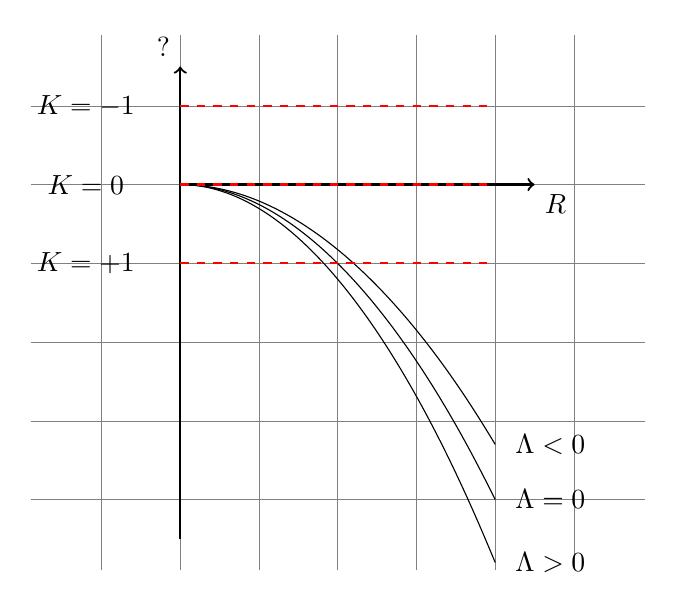
\begin{tikzpicture}
\draw[step=1cm,gray,very thin] (-1.9,-4.9) grid (5.9,1.9);
\draw[thick,->] (0,0) -- (4.5,0) node[anchor=north west] {$R$};
\draw[thick,->] (0,-4.5) -- (0,1.5) node[anchor=south east] {?};
\draw (0,0) parabola (4,-4);
\draw (0,0) parabola (4,-3.3);
\draw (0,0) parabola (4,-4.8);

\draw[red,thick,dashed] (0,1) -- (4,1);
\draw[red,thick,dashed] (0,0) -- (4,0);
\draw[red,thick,dashed] (0,-1) -- (4,-1);

\coordinate (A) at (0,1);
\coordinate (B) at (0,0);
\coordinate (C) at (0,-1);
\node[xshift=-1.2cm] at (A) {$K=-1$};
\node[xshift=-1.2cm] at (B) {$K=0$};
\node[xshift=-1.2cm] at (C) {$K=+1$};

\coordinate (AA) at (4,-3.3);
\coordinate (BB) at (4,-4);
\coordinate (CC) at (4,-4.8);
\node[xshift=0.7cm] at (AA) {$\Lambda<0$};
\node[xshift=0.7cm] at (BB) {$\Lambda=0$};
\node[xshift=0.7cm] at (CC) {$\Lambda>0$};
\end{tikzpicture}
\end{center}




\end{enumerate}

\section{Quantum Mechanics}
\subsection{{\sc Feynman, Hibbs} - Quantum mechanics and path integrals 2ed}
\subsubsection{2.1}
With $\dot x=0$ and $\dot x=$const we see
\begin{align}
    S&=\int_{t_a}^{t_b}L dt\\
    &=\frac{m}{2}\int_{t_a}^{t_b}\dot x^2 dt\\
    &=\frac{m}{2}\left[\left.\dot x x\right|_{t_a}^{t_b}-\int_{t_a}^{t_b} x\ddot xdt\right]\\
    &=\frac{m}{2}\frac{x_b-x_a}{t_b-t_b}(x_b-x_a)\\
     &=\frac{m}{2}\frac{(x_b-x_a)^2}{t_b-t_b}
\end{align}

\subsubsection{2.1}
With the solution of the equation of motion 
\begin{align}
    \ddot x+\omega^2x=0 &\quad\rightarrow\quad x=x_0\sin(\omega t+\varphi_0)=(x_0\cos\varphi_0)\sin \omega t+(x_0\sin\varphi_0)\cos\omega t\\
    &\quad\rightarrow\quad \dot x=(x_0\omega\cos\varphi_0)\cos \omega t-(x_0\omega\sin\varphi_0)\sin\omega t
\end{align}
then with ($x_a,x_b,t_a,t_b$) we can solve for $x_0$ and $\varphi_0$
\begin{align}
    x_0\cos\varphi_0
    &=\frac{x_a\cos\omega t_b-x_b\cos\omega t_a}{\cos\omega t_b\sin\omega t_a-\cos\omega t_a\sin\omega t_b}\\
    &=\frac{x_a\cos\omega t_b-x_b\cos\omega t_a}{\sin\omega(t_a-t_b)}\\
    x_0\sin\varphi_0&=-\frac{x_a\frac{\sin\omega t_b}{\sin\omega t_a}-x_b\tan\omega t_a}{-\sin\omega t_b+\cos\omega t_b\tan\omega t_a}\\
    &=\frac{x_b\sin\omega t_a-x_a\sin\omega t_b}{\sin\omega(t_a-t_b)}
\end{align}
and therefore
\begin{align}
    v_a&=\frac{x_a\cos\omega t_b-x_b\cos\omega t_a}{\sin\omega(t_a-t_b)}\sin\omega t_a+\frac{x_b\sin\omega t_a-x_a\sin\omega t_b}{\sin\omega(t_a-t_b)}\sin\omega t_a\\
    &=-\frac{1}{\sin\omega T}\left[(x_a\cos\omega t_b-x_b\cos\omega t_a)\sin\omega t_a+(x_b\sin\omega t_a-x_a\sin\omega t_b)\sin\omega t_a\right]\\
    &=-\frac{1}{\sin\omega T}\left[x_a(\cos\omega t_b\sin\omega t_a-\sin\omega t_a\sin\omega t_b)+x_b(\sin^2\omega t_a-\cos\omega t_a\sin\omega t_a)\right]\\
    v_b&=\frac{x_a\cos\omega t_b-x_b\cos\omega t_a}{\sin\omega(t_a-t_b)}\sin\omega t_b+\frac{x_b\sin\omega t_a-x_a\sin\omega t_b}{\sin\omega(t_a-t_b)}\sin\omega t_b\\
    &=-\frac{1}{\sin\omega T}\left[x_a(\cos\omega t_b\sin\omega t_b-\sin^2\omega t_b)+x_b(\sin\omega t_a\sin\omega t_b-\cos\omega t_a\sin\omega t_b)\right]
\end{align}
Now we can write
\begin{align}
    S&=\int_{t_a}^{t_b}L dt\\
    &=\frac{m}{2}\int_{t_a}^{t_b}(\dot x^2-\omega^2x^2) dt\\
    &=\frac{m}{2}x_0^2\omega^2\int_{t_a}^{t_b}dt\left(\cos^2(\omega t+\varphi)-\sin^2(\omega t+\varphi)\right)\\
    &=\frac{m}{2}x_0^2\omega^2\int_{t_a}^{t_b}dt\cos(2[\omega t+\varphi])\\
    &=\frac{m}{4}x_0^2\omega\sin(2[\omega t+\varphi])|_{t_a}^{t_b}\\
    &=\frac{m}{2}x_0^2\omega\sin(\omega t+\varphi)\cos(\omega t+\varphi)|_{t_a}^{t_b}\\
    &=\frac{m}{2} x \dot x|_{t_a}^{t_b}\\
    &=\frac{m}{2}(x_bv_b-x_av_a)\\
    &=\frac{m\omega}{2\sin\omega T}\left[(x_a^2+x_b^2)\cos\omega T-2x_ax_b\right]
\end{align}

\subsection{{\sc Straumann} - Quantenmechanik 2ed}
\subsubsection{2.1 - Spectral oscillator density}
The vanishing electrical field in the surface requires for each standing wave
\begin{align}
    k_i=\frac{\pi}{L}n_i. 
\end{align}
and
\begin{align}
    k^2&=k_x^2+k_y^2+k_z^2\\
    \Delta V&=\frac{\pi^3}{L^3}.
\end{align}
With $k=2\pi/\lambda = \omega/c$ we have $dk=\frac{d\omega}{c}$ and the volume of a sphere in $k$-space is given by
\begin{align}
    V(k)&=\frac{4}{3}\pi k^3\\
    dV&=4\pi k^2 dk=4\pi \frac{\omega^2}{c^2} \frac{d\omega}{c} 
    =4\pi (2\pi)^3\frac{\nu^2}{c^3} d\nu 
\end{align}
The number of oscillator are then given by the number of points in the positive quadrant (all $k_i$ positive) time two (polarization)
\begin{align}
    dN(\nu)=2\frac{V(\nu)/8}{\Delta V}=L^3 \frac{8\pi}{c^3}\nu^2d\nu
\end{align}

\subsubsection{2.2 - Energy variance of the harmonic oscillator}
First we obtain an expression for $T$
\begin{align}
    E=\frac{h\nu}{e^{h\nu/kT}-1}\quad\rightarrow\quad\frac{h\nu}{kT}=\ln\left(\frac{h\nu}{E}+1\right)
\end{align}
which we can use in
\begin{align}
    \frac{dS}{dE}=\frac{1}{T}=\frac{k}{h\nu}\ln\left(\frac{h\nu}{E}+1\right)
\end{align}
and take one more derivative
\begin{align}
    \frac{d^2S}{dE^2}&=-\frac{k}{h\nu}\frac{\frac{h\nu}{E^2}}{\frac{h\nu}{E}+1}\\
    &=-k\frac{1}{ h\nu E+E^2}.
\end{align}
Now we see
\begin{align}
    \langle(\Delta E)^2\rangle=E^2+E h \nu.
\end{align}

\subsubsection{3.6 - 1D molecular potential}
With the given coordinate transformation we get for the single terms
\begin{align}
    e^{-\alpha x}&=\frac{\alpha\hbar\xi}{2\sqrt{2mA}}\\
    e^{-2\alpha x}&=\frac{(\alpha\hbar\xi)^2}{8mA}\\
    \frac{\partial}{\partial x}&=\frac{\partial\xi}{\partial x}\frac{\partial}{\partial\xi}\\
    &=-\alpha\xi\frac{\partial}{\partial\xi}\\
    \frac{\partial^2}{\partial x^2}&=\frac{\partial^2\xi}{\partial x^2}\frac{\partial}{\partial\xi}+\left(\frac{\partial\xi}{\partial x}\right)^2\frac{\partial^2}{\partial\xi^2}\\
    &=\alpha^2\xi\frac{\partial}{\partial\xi}+(\alpha\xi)^2\frac{\partial^2}{\partial\xi^2}
\end{align}
and combined
\begin{align}
    -\frac{\hbar^2}{2m}\partial_{xx}\psi+A(e^{-2\alpha x}-2e^{-\alpha x})\psi=E\psi\\
    -\frac{\hbar^2}{2m}\left(\alpha^2\xi\frac{\partial}{\partial\xi}+(\alpha\xi)^2\frac{\partial^2}{\partial\xi^2}\right)\psi+A\left(\frac{(\alpha\hbar\xi)^2}{8mA}-2\frac{\alpha\hbar\xi}{2\sqrt{2mA}}\right)\psi=E\psi\\
    \left(\alpha^2\xi\frac{\partial}{\partial\xi}+(\alpha\xi)^2\frac{\partial^2}{\partial\xi^2}\right)\psi-\frac{2mA}{\hbar^2}\left(\frac{(\alpha\hbar\xi)^2}{8mA}-2\frac{\alpha\hbar\xi}{2\sqrt{2mA}}\right)\psi=-\frac{2mE}{\hbar^2}\psi\\
    \left(\frac{1}{\xi}\frac{\partial}{\partial\xi}+\frac{\partial^2}{\partial\xi^2}\right)\psi-\frac{2mA}{\alpha^2\xi^2\hbar^2}\left(\frac{(\alpha\hbar\xi)^2}{8mA}-2\frac{\alpha\hbar\xi}{2\sqrt{2mA}}\right)\psi=-\frac{2mE}{\hbar^2\alpha^2\xi^2}\psi\\
    \left(\frac{1}{\xi}\frac{\partial}{\partial\xi}+\frac{\partial^2}{\partial\xi^2}\right)\psi+\left(-\frac{1}{4}+\frac{\sqrt{2mA}}{\alpha\hbar\xi}\right)\psi=-\frac{2mE}{\hbar^2\alpha^2\xi^2}\psi\\
    \left(\frac{1}{\xi}\frac{\partial}{\partial\xi}+\frac{\partial^2}{\partial\xi^2}\right)\psi+\left(-\frac{1}{4}+\frac{n+s+\frac{1}{2}}{\xi}\right)\psi=\frac{s^2}{\xi^2}\psi\\
    \left(\frac{\partial^2}{\partial\xi^2}+\frac{1}{\xi}\frac{\partial}{\partial\xi}\right)\psi+\left(-\frac{1}{4}+\frac{n+s+\frac{1}{2}}{\xi}-\frac{s^2}{\xi^2}\right)\psi=0.
\end{align}
The units of $\xi$ is $\sqrt{\text{kg}\cdot \text{J}}/\text{m}^{-1}\text{Js}=1$ so $\xi$ in dimensionless.
\begin{enumerate}
    \item Case $\xi\gg 1$ ($x\rightarrow-\infty$)
    Dropping all $1/\xi$ terms
    \begin{align}
        \psi''-\frac{1}{4}\psi=0\quad\rightarrow\quad\psi=c_1 e^{\xi/2}+c_2 e^{-\xi/2}
    \end{align}
    \item Case $0<\xi\ll 1$ ($x\rightarrow+\infty$)
    Ansatz $\psi\sim\xi^m$
    \begin{align}
        m(m-1)\xi^{m-2}+m\xi^{m-2}-\frac{1}{4}\xi^m+\left(n+s+\frac{1}{2}\right)\xi^{m-1}-s^2\xi^{m-2}=0\\
        \left[(m^2-s^2)-\frac{1}{4}\xi^2+\left(n+s+\frac{1}{2}\right)\xi\right]\xi^{m-2}=0
    \end{align}
    which for small $\xi$ becomes
    \begin{align}
        (m^2-s^2)\xi^{m-2}=0 \quad\rightarrow\quad\psi=\xi^{\pm s}
    \end{align}
\end{enumerate}
With the two asymptotics we can make a physically sensible ansatz for a full solutions $\psi=\xi^s e^{-\xi/2}u(\xi)$ which leads to
\begin{align}
    \xi u''+(2s+1-\xi)u'+n u=0
\end{align}
To solve this equation we use the Sommerfeld polynomial method
\begin{align}
    u=\sum_ka_k\xi^k\quad\rightarrow\quad
    &\sum_kk(k-1)a_k\xi^{k-1}+(2s+1)ka_k\xi^{k-1}-ka_k\xi^k+na_k\xi^k=0\\
    &\sum_k(k+1)ka_{k+1}\xi^{k}+(2s+1)(k+1)a_{k+1}\xi^{k}-ka_k\xi^k+na_k\xi^k=0\\
    &a_{k+1}=\frac{k-n}{(k+1)(2s+1+k)}a_k.
\end{align}
The requirement for the series to cut off (making $u$ a finite order polynomial) is $n_k=k$. The energies of the bound states are therefore
\begin{align}
    E_k&=-\frac{\alpha^2\hbar^2}{2m}s_k^2\\
    &=-\frac{\alpha^2\hbar^2}{2m}\left[\frac{\sqrt{2mA}}{\alpha\hbar}-(k+1/2)\right]^2\\
    &=-A\left[1-\frac{\alpha\hbar}{\sqrt{2mA}}(k+1/2)\right]^2
\end{align}
where the only valid $k$ are the ones where $E_k$ is in $[-A,0]$.


\subsection{{\sc Schwinger} - Quantum Mechanics Symbolism of Atomic Measurements}
\subsubsection{2.1}
Observe
\begin{align}
    \int_{-\infty}^\infty\left(\theta(x+a)+\theta(a-x)\right)e^{ikx}dx
    &=\int_{-a}^ae^{ikx}dx\\
    &=\frac{1}{ik}\left(e^{ika}-e^{-ika}\right)\\
    &=2a \frac{\sin ka}{ka}
\end{align} 

\begin{align}
    \lim_{P\rightarrow\infty}\int_{-\infty}^\infty\frac{d\chi}{\pi}\frac{\sin\chi}{\chi}e^{ik\left(q'+\frac{\chi}{P}\right)}=\frac{1}{\pi}e^{ikq'}\lim_{P\rightarrow\infty}\int_{-\infty}^\infty d\chi\frac{\sin\chi}{\chi}e^{i\frac{k}{P}\chi}
\end{align} 



\subsection{{\sc Weinberg} - Quantum Mechanics 2nd edition}
\subsubsection{1.1}
\begin{itemize}
\item The solution of for a free particle in the interval $-a<x<a$ is given by
\begin{align}
    \left[-\frac{\hbar^2}{2M}\frac{d^2}{dx^2}-E\right]\phi&=0\\
    \left[\frac{d^2}{dx^2}+\frac{2ME}{\hbar^2}\right]\phi&=0\\
    \rightarrow\phi&=A\sin\left(\frac{\sqrt{2ME}}{\hbar}x\right)+B\cos\left(\frac{\sqrt{2ME}}{\hbar}x\right)
\end{align}    
with the two boundary conditions
\begin{align} 
A\sin\left(\frac{\sqrt{2ME}}{\hbar}(-a)\right)+B\cos\left(\frac{\sqrt{2ME}}{\hbar}(-a)\right)=0\\
A\sin\left(\frac{\sqrt{2ME}}{\hbar}a\right)+B\cos\left(\frac{\sqrt{2ME}}{\hbar}a\right)=0.
\end{align}
The possible energy eigenvalues are therefore
\begin{align}
    A=0,\quad\frac{\sqrt{2ME_{2n+1}}}{\hbar}a=(2n+1)\frac{\pi}{2}
    &\quad\rightarrow\quad E_{2n+1}=\frac{\pi^2\hbar^2}{8Ma^2}(2n+1)^2\\
    &\quad\rightarrow\quad
    \phi=\frac{1}{\sqrt{a}}\cos\left(x\frac{\pi}{2a}(2n+1)\right)
\end{align}   
    
\begin{align}    
    B=0,\quad\frac{\sqrt{2ME_{2n}}}{\hbar}a=2n\frac{\pi}{2}
    &\quad\rightarrow\quad E_{2n}=\frac{\pi^2\hbar^2}{8Ma^2}(2n)^2\\
    &\quad\rightarrow\quad
    \phi=\frac{1}{\sqrt{a}}\sin\left(x\frac{\pi}{2a}(2n)\right)
\end{align}
where we calculated the normalization via
\begin{align}
    \int_{-a}^a\sin^2(kx)dx
    &=\int_{-a}^a(1-\cos^2(kx))dx\\
    &=2a-\int_{-a}^a\cos^2(kx)dx\quad\rightarrow\int_{-a}^a\sin^2(kx)dx=a.
\end{align}

\item Lets first calculate the normalization
\begin{align}
    \int_{-a}^a(a^2-x^2)^2dx
    &=\left.a^4x-2a^2\frac{x^3}{3}+\frac{x^5}{5}\right|_{-a}^a\\
    &=a^4(2a)-\frac{2}{3}a^2(16a^3)+\frac{1}{5}(64a^5)\\
    &=\left(2-\frac{4}{3}+\frac{2}{5}\right)a^5=\frac{16}{15}a^5
\end{align}
and then obtain
\begin{align}
    \int_{-a}^a \frac{1}{\sqrt{\frac{16a^5}{15}}} \left(a^2-x^2\right)\frac{1}{\sqrt{a}} \cos \left(\frac{\pi  x}{2 a}\right)dx=\frac{8\sqrt{15}}{\pi^3}
\end{align}
\end{itemize}

\subsubsection{1.2}
\begin{itemize}
\item We can write the Hamiltonian as
\begin{align}
    H&=\frac{\vec{P}^2}{2M}+\frac{M\omega_0^2}{2}\vec{X}^2\\
    &=\sum_{k=1}^3\frac{p_k^2}{2M}+\frac{M\omega_0^2}{2}x_k^2
\end{align}
the energy is therefore given by
\begin{align}
    E_{n_1,n_2,n_3}&=\hbar\omega_0\left(n_1+n_2+n_3+\frac{3}{2}\right)\\
    N_{n=n_1+n_2+n_3}&=\sum_{k=0}^{n}(k+1)\\
    &=\frac{n(n+1)}{2}+n+1\\
    &=\frac{(n+1)(n+2)}{2}
\end{align}

\item With (1.4.5), (1.4.15) and $\omega_{01}=\omega_0$ we have
\begin{align}
    \vec{x}]_{01}&=e^{i\omega_0 t}\sqrt{\frac{\hbar}{2M\omega_0}}\\
    A_{n=1}^{n=0}&=\frac{4e^2\omega_0^3}{3c^3\hbar}\left|[\vec{x}]_{01}\right|^2\\
    &=\frac{2e^2\omega_0^2}{3c^3M}
\end{align}
where with (1.4.15).
\end{itemize}

\subsection{{\sc Sakurai, Napolitano} - Modern Quantum Mechanics 3rd ed}
\subsubsection{5.1 Harmonic oscillator with linear perturbation}
The Hamiltonians are given by
\begin{align}
\hat{H}_0&=-\frac{\hbar^2}{2m}\frac{d^2}{dx^2}+\frac{1}{2}m\omega_o^2x^2\\
\hat{H}_1&=bx
\end{align}
We remember
\begin{align}
\phi_0(x)&=\left(\frac{m\omega_0}{\pi\hbar}\right)^{1/4}e^{-m\omega_0x^2/2\hbar}\\
E_0&=\frac{1}{2}\hbar\omega_0\\
\phi_n(x)&=\frac{1}{\sqrt{2^n n!}}\left(\frac{m\omega_0}{\pi\hbar}\right)^{1/4}e^{-m\omega_0x^2/2\hbar}H_n\left(\sqrt{\frac{m\omega_0}{\hbar}}x\right)\\
E_n&=\hbar\omega_0\left(n+\frac{1}{2}\right)
\end{align}
\begin{enumerate}
\item Time independent perturbation theory gives
\begin{align}
\Delta E_n^{(1)}&=\langle n^{(0)}|\hat{H}_1|n^{(0)}\rangle\\
\Delta E_0^{(1)}&=\langle 0^{(0)}|\hat{H}_1|0^{(0)}\rangle =0
\end{align}
The first order energy shift vanishes because of the wave function is even and $H_1$ is odd.
For the first order perturbation of the wave function we observe
\begin{align}
H_1(x)&=2xH_0(x)\quad\rightarrow\quad\hat{H}_1|0^{(0)}\rangle=\frac{b}{2}\sqrt{2}\sqrt{\frac{\hbar}{m\omega_0}}|1^{(0)}\rangle\\
\langle m^{(0)}|n^{(0)}\rangle&=\delta_{nm}
\end{align}
Now we can calculate  
\begin{align}
|n^{(1)}\rangle&=\sum_{k\neq n}\frac{\langle k^{(0)}|\hat{H}_1|n^{(0)}\rangle}{E_n^{(0)}-E_k^{(0)}}|k^{(0)}\rangle\\
|0^{(1)}\rangle&=\frac{\langle 0^{(0)}|\hat{H}_1|1^{(0)}\rangle}{E_0^{(0)}-E_1^{(0)}}|1^{(0)}\rangle\\
&=-\frac{1}{\hbar\omega_0}b\sqrt{\frac{\hbar}{2m\omega_0}}|1^{(0)}\rangle\\
&=-b\sqrt{\frac{1}{2m\hbar\omega_0^3}}|1^{(0)}\rangle
\end{align}
Second order enegy perturbation
\begin{align}
\Delta E_n^{(2)}&=\langle n^{(0)}|\hat{H}_1|n^{(1)}\rangle=\sum_{k\neq n}\frac{|\langle k^{(0)}|\hat{H}_1|n^{(0)}\rangle|^2}{E_n^{(0)}-E_k^{(0)}}\\
\Delta E_0^{(2)}&=\langle 0^{(0)}|\hat{H}_1|0^{(1)}\rangle\\
&=b\sqrt{\frac{\hbar}{2m\omega_0}}\langle 1^{(0)}|0^{(1)}\rangle\\
&=b\sqrt{\frac{\hbar}{2m\omega_0}}\langle 1^{(0)}|\left(-b\sqrt{\frac{1}{2m\hbar\omega_0^3}}\right)|1^{(0)}\rangle\\
&=-b^2\frac{1}{2m\omega_0^2}
\end{align}
\item The linear perturbation does not change the shape of the potential - only shifts the minimum 
\begin{align}
 V(x)&=\frac{m\omega_0^2}{2}x^2+bx=\frac{m\omega_0^2}{2}\left(x+\frac{b}{m\omega_0^2}\right)^2-\frac{b^2}{2m\omega_0^2}\\
\Delta E^{(\infty)}&=-\frac{b^2}{2m\omega_0^2} 
\end{align}
\end{enumerate}
So the second order gives the exact result - interesting to see if higher orders would all  vanish or give oscillating contributions.  

\subsubsection{5.2 Potential well with linear slope}
We will treat the slope as a perturbation with
\begin{align}
\hat{H}_1=\frac{V}{L}x
\end{align} 
Therefore the unperturbed wave functions are given by
\begin{align}
\phi_n=\sqrt{\frac{2}{L}}\sin\frac{n\pi x}{L}\qquad
E_n=\frac{\pi^2\hbar^2}{2mL^2}n^2
\end{align}
Then
\begin{align}
\Delta E_n^{(1)}
&=\langle n^{(0)}|\hat{H}_1|n^{(0)}\rangle\\
&=\frac{V}{L}\frac{2}{L}\int_0^L x\sin^2\frac{n\pi x}{L}dx\\
&=\frac{2V}{L^2}\int_0^L x\sin^2\frac{n\pi x}{L}dx\\
&=\frac{2V}{L^2}\int_0^L x\left(1-\cos^2\frac{n\pi x}{L}\right)dx\\
&=\frac{2V}{L^2}\frac{L^2}{2}-\Delta E_n^{(1)}
\end{align}
meaning $\Delta E_n^{(1)}=V/2$.

\subsubsection{5.3 Relativistic perturbation}
We can approximate the kinetic energy by
\begin{align}
E&=\sqrt{m^2c^4+p^2c^2}\\
&\approx mc^2+\frac{p^2}{2m}-\frac{p^4}{8m^3c^2}+\frac{p^6}{16m^5c^4}+\cdots\\
&=mc^2+\frac{mc^2}{2}\frac{p^2}{m^2c^2}-\frac{mc^2}{8}\frac{p^4}{m^4c^4}+\cdots\\
&=mc^2\left(1+\frac{1}{2}\beta^2-\frac{1}{8}\beta^4+\cdots\right)
\end{align}
so
\begin{align}
\hat{H}_0&=-\frac{\hbar^2}{2m}\frac{d^2}{dx^2}+\frac{1}{2}m\omega^2x^2\\
\hat{H}_1&=-\frac{1}{8m^3c^2}p^4=-\frac{\hbar^4}{8m^3c^2}\frac{d^4}{dx^4}
\end{align}
and we remember
\begin{align}
\phi_0(x)&=\left(\frac{m\omega}{\pi\hbar}\right)^{1/4}e^{-m\omega x^2/2\hbar}\\
E_0&=\frac{1}{2}\hbar\omega_0
\end{align}
then
\begin{align}
\Delta E_0^{(1)}&=\langle 0^{(0)}|\hat{H}_1|0^{(0)}\rangle\\
&=-\frac{\hbar^4}{8m^3c^2}\int_{-\infty}^\infty\phi_0(x)^*\frac{d^4}{d^4x}\phi_0(x)dx\\
&=-\frac{3\hbar^2\omega^2}{32mc^2}
\end{align}

\subsubsection{5.4 Diatomic atomic rotor}
Hamiltonian of the problem is given by
\begin{align}
H=\frac{L^2}{2I}\quad\rightarrow\quad\hat{H}&=-\frac{\hbar^2}{2I}\frac{d^2}{d\varphi^2}
\end{align}
with the unperturbed solutions
\begin{align}
\phi_n^{(0)}&=C e^{in\phi}\qquad E_n^{(0)}=\frac{\hbar^2n^2}{2I}
\end{align}
where only $E_0$  is non-degenerate (all other are double degenerated). 
For the perturbation we use the Hamiltonian
\begin{align}
\hat{H}_1&=Ed\cos\varphi
\end{align}
Hmmm....


\subsubsection{5.6 Two dimensional potential well}
As the problem separates 
\begin{align}
\left(\hat{H}_x+\hat{H}_y\right)\phi_x\phi_y=(E_x+E_y)\phi_x\phi_y\\
\phi_y\hat{H}_x\phi_x+\phi_x\hat{H}_y\phi_y=(E_x+E_y)\phi_x\phi_y\\
\frac{\hat{H}_x\phi_x}{\phi_x}+\frac{\hat{H}_y\phi_y}{\phi_y}=(E_x+E_y)
\end{align}
the wave function can be written as a product of the 1-dimensional wave functions
\begin{align}
\phi_{n_x,n_y}&=\sqrt{\frac{2}{L}}\sqrt{\frac{2}{L}}\sin\left(\frac{n_x\pi}{L}x\right)\sin\left(\frac{n_y\pi}{L}y\right)\\
E_{n_x,n_y}&=\frac{\pi^2\hbar^2}{2mL^2}(n_x^2+n_y^2)
\end{align}
So 
\begin{align}
\phi_{1,1}\quad\rightarrow\quad E_{1,1}&=2\frac{\pi^2\hbar^2}{2mL^2}\\
\phi_{2,1},\phi_{1,2}\quad\rightarrow\quad E_{2,1}&=5\frac{\pi^2\hbar^2}{2mL^2}\\
\phi_{2,2}\quad\rightarrow\quad E_{1,1}&=8\frac{\pi^2\hbar^2}{2mL^2}
\end{align}
for the non-degenerated levels $E_{1,1}$ and $E_{2,2}$ we get
\begin{align}
\Delta E_{1,1}^{(1)}&=\langle 1,1^{(0)}|\hat{H}_1|1,1^{(0)}\rangle\\
&=\frac{1}{4}\lambda L^2\\
\Delta E_{2,2}^{(1)}&=\langle 2,2^{(0)}|\hat{H}_1|2,2^{(0)}\rangle\\
&=\frac{1}{4}\lambda L^2
\end{align}
and for the degenerated levels $E_{1,2}/E_{2,1}$ we get
\begin{align}
H=
\begin{pmatrix}
\langle 1,2^{(0)}|\hat{H}_1|1,2^{(0)}\rangle & \langle 1,2^{(0)}|\hat{H}_1|2,1^{(0)}\rangle\\
\langle 2,1^{(0)}|\hat{H}_1|1,2^{(0)}\rangle & \langle 2,1^{(0)}|\hat{H}_1|2,1^{(0)}\rangle
\end{pmatrix}
\end{align}
with
\begin{align}
H_{aa}&=\langle 1,2^{(0)}|\hat{H}_1|1,2^{(0)}\rangle=\frac{\lambda L^2}{4}\\
H_{ab}&=\langle 1,2^{(0)}|\hat{H}_1|2,1^{(0)}\rangle=\frac{256\lambda L^2}{81\pi^4}\\
H_{bb}&=\langle 2,1^{(0)}|\hat{H}_1|2,1^{(0)}\rangle=\frac{\lambda L^2}{4}
\end{align}
and $\hat{H}_1=\lambda x y$ Diagonalising the matrix $H$ gives the perturbation
\begin{align}
\Delta E_{12,21}^{(1)}=\frac{\lambda L^2}{4}-\frac{256\lambda L^2}{81\pi^4}\\
\Delta E_{12,21}^{(1)}=\frac{\lambda L^2}{4}+\frac{256\lambda L^2}{81\pi^4}\\
\end{align}


\subsubsection{5.8 Quadratically perturbed harmonic oscillator}
\begin{align}
\hat{H}_1=\epsilon\frac{1}{2}m\omega^2x^2
\end{align}

\begin{align}
H_0(x)&=1\\
H_2(x)&=4x^2-2\quad\rightarrow\quad x^2=\frac{H_2}{4}+\frac{1}{2}
\end{align}


\subsubsection{8.1 Natural units}
\begin{enumerate}
\item Proton Mass
\begin{align}
      E_p=m_pc^2/e=0.937\text{GeV}
\end{align}
\item With $\Delta p\cdot\Delta x\ge\hbar/2$ and $E=\sqrt{m^2c^4+p^2c^2}\approx pc$
\begin{align}
	E=\Delta p c/e=98.6\text{MeV}
\end{align}
Alternatively we have $E=\frac{\hbar c}{e\cdot dx}$ meaning $1\text{fm}=\frac{1}{197.3\text{MeV}}$ and therefore
\begin{align}
	E=\frac{\hbar}{2\cdot\Delta x}c=197.3/2\text{MeV}
\end{align}
\item Solving for $\alpha,\beta,\gamma$
\begin{align}
	M_P
	&=G^\alpha c^\beta \hbar^\gamma\\
	&=\left(\frac{\text{Nm}^2}{\text{kg}^2}\right)^\alpha\left(\frac{\text{m}}{\text{s}}\right)^\beta\left(\text{Js}\right)^\gamma\\
	&=\sqrt{\frac{\hbar c}{G}}\\
	E_P&=\sqrt{\frac{\hbar c}{G}}c^2\frac{1}{e}=1.22\cdot10^{19}\text{GeV}
\end{align}
\end{enumerate}
\subsubsection{8.2 Minkowski Metric}
The definition implies that $\eta_{\lambda\nu}$ is the inverse of $\eta^{\lambda\nu}$ - simple calculation shows that they are identical. Now we can calculate
\begin{align}
\eta^{\mu\lambda}\eta^{\nu\sigma}\eta_{\lambda\sigma}
&=\eta^{\nu\sigma}\delta^\mu_\sigma\\
&=\eta^{\nu\mu}
\end{align}
and
\begin{align}
a^\mu b_\mu=a_\alpha\eta^{\alpha\mu}b^\beta\eta_{\beta\mu}=a_\alpha b^\beta\delta^\alpha_\beta=a_\alpha b^\alpha
\end{align}


\subsection{{\sc Bethe, Jackiw} - Intermediate Quantum Mechanics}
\subsubsection{1.1 Atomic units}
Set $\hbar=e=m_e=1$ and $a_B=\frac{4\pi\varepsilon_0\hbar^2}{m_ee^2}=1$ then $4\pi\varepsilon_0=1$ and therefore $\alpha=\frac{e^2}{4\pi\varepsilon_0\hbar c}=1/c$
\begin{enumerate}
\item energy: $E_{1s}=\frac{1}{2}m_ec^2\alpha^2$ therefore 1 a.u. = $2\times13.6$eV
\item momentum: $p=m_e c$ therefore 1 a.u. = $2\cdot 10^{-31}\text{kg}\times 3\cdot 10^8\text{m/s}^2=2.73\cdot10^{-22}$J
\item angular momentum: $L=\hbar$ therefore 1 a.u. = $1.04\cdot10^{-34}$Js 
\end{enumerate}



\section{General Physics}

\subsection{{\sc Feynman} - Feynman Lectures on Physics}
\subsubsection{Section G1-1 - 1961 Sep 28 (1.16)}
\subsubsection{Section G1-2 - 1961 Sep 28 (1.15)}
\begin{enumerate}[label=(\alph*)]
\item  We use the Penman equation to estimate the specific evaporation rate
\begin{align}
    \frac{dm}{dA dt}
    &=\frac{m R_n + \rho_\text{air}c_p (\delta e)g_a}{\lambda_v(m+\gamma)}\\
    &=\frac{m R_n + \rho_\text{air}c_p (\delta e)g_a}{\lambda_v(m+\frac{c_p p}{\lambda_v MW_\text{ratio}})}\\
    &\approx\frac{m R_n}{\lambda_v(m+\frac{c_p p}{\lambda_v MW_\text{ratio}})}.
\end{align}
The total time is then given by
\begin{align}
    t&=\frac{M}{\frac{dm}{dA dt}A}\\
    &=\frac{M}{\frac{dm}{dA dt}\pi r^2}\\
    &=\frac{M\lambda_v(m+\frac{c_p p}{\lambda_v MW_\text{ratio}})}{\pi r^2 m R_n }
\end{align}
with vapor the water vapor pressure
\begin{align}
    p_\text{vap}=\frac{101325\text{Pa}}{760} \exp\left[20.386 - \frac{5132K}{T}\right]
\end{align}
the slope of the saturation vapor pressure
\begin{align}
    m=\frac{\partial p_\text{vap}}{\partial T}=...
\end{align}
the air heat capacity $c_p=1.012\text{J}\text{kg}^{-1}\text{K}^{-1}$, the latent heat of vaporization $\lambda_v=2.26\cdot10^6 \text{J}\text{kg}^{-1}$, the net irradiance $R_n=150\text{Wm}^{-2}$ (average day/night partly shade), the ratio molecular weight of water vapor/dry air $MW_\text{ratio}=0.622$, the pressure $p=10^5\text{Pa}$, the temperature $T= 298\text{K}$, the water weight $M=0.5\text{kg}$ and the radius of the glass $r=0.04\text{m}$. This results in $t=26$ days.

\item With the molar mass of water $m_{H2O}=18\,\text{g}\cdot\text{mol}^{-1}$

\begin{align}
    N&=\frac{dm}{dA dt} \frac{N_A}{m_{H20}}\\
    &=\frac{m R_n}{\lambda_v(m+\frac{c_p p}{\lambda_v MW_\text{ratio}})}\frac{N_A}{m_{H20}}\\
    &=1.47\cdot10^{17}\text{cm}^{-1}\text{s}^{-1}
\end{align}

\item The total mass of water vaporizing on earth in one year is
\begin{align}
    M_\text{1y prec}=\varepsilon_\text{ocean} 4\pi R_E^2  \frac{dm}{dA dt} t_{1y}.
\end{align}
with $\varepsilon_\text{ocean}=0.7$. In equilibrium this must be equal to the total amount of precipitation. So the average rainfall height is 
\begin{align}
    h&=\frac{M_\text{1y prec}}{4\pi R_E^2\rho_\text{H2O}}\\
    &=\frac{\varepsilon_\text{ocean}t_{1y}}{\rho_\text{H2O}} \frac{dm}{dA dt}\\
    &=947\text{mm}.
\end{align}
which seems reasonable (given that the solar constant is $1,361\text{Wm}^{-2}$ the estimate of $R_n=150\text{Wm}^{-2}$ seems ok).
\end{enumerate}

\subsubsection{Section G-1 - 1961 Oct 5 (?.??)}
\begin{enumerate}[label=(\alph*)]
    \item $\sqrt{s/g}$
    \item $mL/T^2$
    \item $\rho g h$
    \item $\sqrt{p/\rho}$
    \item $gT$ (need to use the period $T$ as $c$ is not a material constant due to strong dispersion)
    \item $\rho g H^2$
    \item $\sqrt{R/g}$ here we assume the hemisphere rests on the table upside down - so it acts like a pendulum 
    \item $\sqrt{FL/m}$
\end{enumerate}

\subsubsection{Section G-2 - 1961 Oct 5 (?.??)}
\begin{enumerate}
    \item Equilibrium is given by condition
    \begin{align}
        m_1g&=m_2g\sin\alpha\\
        &=m_2g\frac{x}{\sqrt{x^2+a^2}}\\
        \rightarrow\quad& m_1^2(x^2+a^2)=m_2^2 x^2\\
        \rightarrow\quad& x=\frac{m_1 a}{\sqrt{m_2^2-m_1^2}}\\
    \end{align}
    \item General consideration
    \begin{center}
    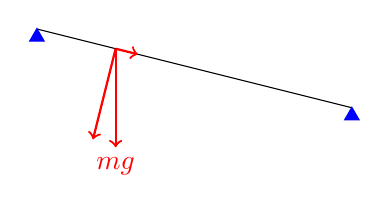
\begin{tikzpicture}
    \draw (-2,1) -- (2,0);
    \node[mark size=3pt,color=blue] at (-2,0.9) {\pgfuseplotmark{triangle*}};
    \node[mark size=3pt,color=blue] at (2,-0.1) {\pgfuseplotmark{triangle*}};
    \draw [->, thick,red] (-1,0.75) -- (-1,-0.5) node[below ]{$mg$};
    \draw [->, thick,red] (-1,0.75) -- (-1+0.28,0.75-0.07);
    \draw [->, thick,red] (-1,0.75) -- (-1-0.25*1.15,0.75-1*1.15);
    \end{tikzpicture}
    \end{center}
    
    \item
    \item
    \item
\end{enumerate}

\subsubsection{Problem Set 3-1 - 1961 Nov 03 (3.16)}
Direct measurement can be done for the
\begin{itemize}
    \item radius of the earth $R_e=6371\text{km}$
    \item orbital period of the moon $T_M=28\text{d}$
    \item angular diameter of the moon $\delta=30'=0.5^\circ$
    \item earths gravitational acceleration $g=9.81\text{ms}^2$
    \item also Sputnik I orbital data can be looked up $a_\text{satellite}=R_E+584\text{km}$ and $T_\text{satellite}=96.2\text{min}$
    \item height difference between low and high tide $\Delta h=1\text{m}$
\end{itemize}

\begin{enumerate}
\item We use Keplers 3rd law
\begin{align}
    \frac{a_M^3}{T_M^2}&=\frac{a_\text{satellite}^3}{T_\text{satellite}^2}\\
    a_M&=a_\text{sat}\left(\frac{T_M}{T_\text{sat}}\right)^{2/3}
\end{align}
then the radius of the moon is given by
\begin{align}
R_M=\frac{a_M}{2}\tan\delta=\frac{a_\text{sat}}{2}\left(\frac{T_M}{T_\text{sat}}\right)^{2/3}\tan\delta
\end{align}
and the mass by
\begin{align}
    m_M&=\rho_M V_M=\frac{4}{3}\pi\rho_M R_M^3\\
    &=\frac{4}{3}\pi\rho_M \left(\frac{a_\text{sat}}{2}\left(\frac{T_M}{T_\text{sat}}\right)^{2/3}\tan\delta \right)^3\\
    &=\frac{1}{6}\pi\rho_M a_\text{sat}^3\left(\frac{T_M}{T_\text{sat}}\right)^2\tan^3\delta \\
    &\approx\frac{1}{6}\pi\rho_E a_\text{sat}^3\left(\frac{T_M}{T_\text{sat}}\right)^2\tan^3\delta 
\end{align}
where we approximated the moon by the earth mass density. From the gravitational law we can obtain the earth density by
\begin{align}
    g&=\frac{F_g}{m}=\frac{Gm_E}{R_E^2}\quad\rightarrow\quad m_E=\frac{gR_E^2}{G}\\
    \rho_E&=\frac{m_E}{V_E}=\frac{m_E}{\frac{4}{3}\pi R_E^3}=\frac{3g}{4\pi G R_E}.
\end{align}
Therefore the mass of the moon is given by
\begin{align}
    m_M&\approx\frac{g}{ 8G R_E} a_\text{sat}^3\left(\frac{T_M}{T_\text{sat}}\right)^2\tan^3\delta \\
    &=1.16\cdot10^{23}\text{kg}.
\end{align}

\item  We use Keplers 3rd law (for the earth-moon system) and the gravitational law for the earth
\begin{align}
    \frac{a_M^3}{T_M^2}&=\frac{G(m_E+m_M)}{4\pi^2}\approx\frac{Gm_E}{4\pi^2}=\frac{a_\text{satellite}^3}{T_\text{satellite}^2}\\
    g&=\frac{F_g}{m}=\frac{Gm_E}{R_E^2}
\end{align}
and obtain
\begin{align}
    \frac{a_\text{satellite}^3}{T_\text{satellite}^2}&=\frac{gR_E^2+Gm_M}{4\pi^2}\\
    m_M&=\frac{4\pi^2}{G}\left(\frac{a_\text{satellite}^3}{T_\text{satellite}^2}-\frac{gR_E^2}{4\pi^2}\right)\\
    &=7.07\cdot10^{21}\text{kg}.
\end{align}
This result is quite sensitive to the satellite orbital data.


\item We will use the earth tidal data. Lets assume circular orbits with $a_E+a_M=D$ which we can justify by observation (as the moon appears to have constant angular diameter). As reference system we use the center of mass of the system

\begin{center}
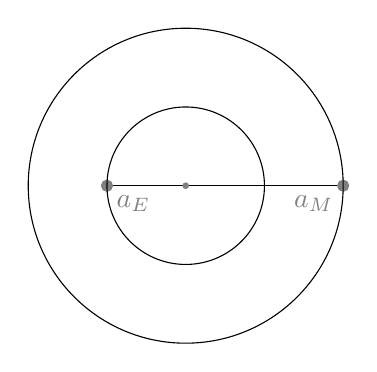
\begin{tikzpicture}
\draw (-1,0) -- (2,0);
\filldraw [gray] (-1,0) circle (2pt) node[below right]{$a_E$};
\filldraw [gray] (2,0) circle (2pt) node[below left]{$a_M$};
\filldraw [gray] (0,0) circle (1pt);
\draw (0,0) circle (2);
\draw (0,0) circle (1);
\end{tikzpicture}
\end{center}
\begin{align}
    m_E\omega^2a_E&=\frac{Gm_Em_M}{D^2}=m_M\omega^2a_M\\
    &\rightarrow a_E=\frac{m_MD}{m_E+m_M}\\
    &\rightarrow \omega^2=\frac{G(m_E+m_M)}{D^3}\\
    &\rightarrow \omega^2a_E^2=\frac{Gm_M^2}{D(m_E+m_M)}\\
    &\rightarrow \frac{R_E}{a_E}=\frac{m_E+m_M}{m_M}\frac{R_E}{D}
\end{align}

\begin{center}
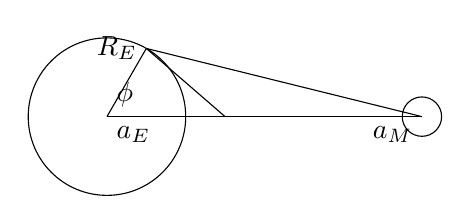
\begin{tikzpicture}
\draw (-2,0) -- (2,0);
\draw (-2,0) circle (1) node[below right]{$a_E$} node[above right]{$\phi$};
\draw (2,0) circle (0.25) node[below left]{$a_M$};
\draw (2,0) -- (-1.5,0.866);
\draw (-2,0) -- (-1.5,0.866) node[left]{$R_E$};
\draw (-0.5,0) -- (-1.5,0.866);
\end{tikzpicture}
\end{center}
The potential is then given by (gravity of moon and earth as well as the centripetal potential around the center of gravity)
\begin{align}
    V&=V_\text{G,moon}+V_\text{G,earth}+V_\text{cent}\\
    &=-\frac{G m_M}{\sqrt{R_E^2+D^2-2DR_E\cos\phi}}-\frac{Gm_E}{R_E}-\frac{1}{2}\omega^2(R_E^2+a_E^2-2a_ER_E\cos\phi)\\
    &=-\frac{Gm_M}{D\sqrt{\left(\frac{R_E}{D}\right)^2+1-2\frac{R_E}{D}\cos\phi}}-\frac{Gm_E}{R_E}-\frac{1}{2}\omega^2a_E^2\left[\left(\frac{R_E}{a_E}\right)^2+1-2\frac{R_E}{a_E}\cos\phi\right]\\
    &\approx-\frac{Gm_M}{D}\left(1+\frac{R_E}{D}\cos\phi+\frac{3}{2}\left(\frac{R_E}{D}\right)^2\cos^2\phi\right)-\frac{Gm_E}{R_E}\\
    &\quad\quad\quad-\frac{1}{2}\omega^2a_E^2\left[\left(\frac{R_E}{a_E}\right)^2+1-2\frac{R_E}{a_E}\cos\phi\right]\\
    &\approx-\frac{Gm_M}{D}\left(1+\frac{R_E}{D}\cos\phi+\frac{3}{2}\left(\frac{R_E}{D}\right)^2\cos^2\phi\right)-\frac{Gm_E}{R_E}\\
    &\quad\quad\quad-\frac{1}{2}\frac{Gm_M^2}{D(m_E+m_M)}\left[\left(\frac{m_E+m_M}{m_M}\frac{R_E}{D}\right)^2+1-2\frac{m_E+m_M}{m_M}\frac{R_E}{D}\cos\phi\right]\\
    &\approx-\frac{Gm_M}{D}-\frac{3Gm_M}{2D}\frac{R_E^2}{D^2}\cos^2\phi-\frac{Gm_E}{R_E}\\
    &\quad\quad\quad-\frac{1}{2}\frac{Gm_M^2}{D(m_E+m_M)}\left[\left(\frac{m_E+m_M}{m_M}\frac{R_E}{D}\right)^2+\frac{m_M^2D^2}{m_M^2D^2}\right]\\
    &\approx-\frac{Gm_M}{D}-\frac{3Gm_M}{2D}\frac{R_E^2}{D^2}\cos^2\phi-\frac{Gm_E}{R_E}-\frac{G}{2}\left[(m_E+m_M)\frac{R_E^2}{D^3}+\frac{m_M^2}{m_E+m_M}\frac{1}{D}\right].
\end{align}
with the angular dependent tidal part
\begin{align}
    V_\text{tidal}&=
    -\frac{3 G R_E^2m_M }{2D^3}\cos ^2\phi.
\end{align}
The tidal water surface would be formed by the the surface $r_\text{surf}(\phi)=R_E+h$ of constant potential. The height difference between low and high tide can then be estimated by 
\begin{align}
   -\frac{3 G R_E^2m_M }{2D^3} 
   &= Gm_E\left(\frac{1}{R_E+h}-\frac{1}{R_E}\right)\\
   &\approx Gm_E\left(\frac{1}{R_E\left(1+\frac{h}{R_E}\right)}-\frac{1}{R_E}\right)\\
   &\approx \frac{Gm_E}{R_E}\left(\left(1-\frac{h}{R_E}\right)-1\right)
\end{align}
which gives
\begin{align}
    h=\frac{3R_E^4}{2D^3}\frac{m_M}{m_E}.
\end{align}
Using the results from above
\begin{align}
    m_E&=\frac{gR_E^2}{G}\\
    \omega^2&=\frac{G(m_E+m_M)}{D^3}\\
    &\quad\rightarrow\quad D^3=\frac{G(m_E+m_M)}{\omega^2}=G(m_E+m_M)\frac{T_M^2}{4\pi^2}
\end{align}
we obtain
\begin{align}
    h=\frac{6\pi^2R_E^4T_M^2}{G(m_E+m_M)T_M^2}\frac{m_M}{m_E}.
\end{align}
and can subsequently solve for $m_M$
\begin{align}
    m_M&=\frac{G h m_E^2 T^2}{6 \pi ^2 R_E^4-G h m_E T^2}\\
    &=\frac{m_E}{\frac{6\pi^2 R_E^4}{G h m_E T^2}-1}\\
    &=\frac{g^2 h T_M^2 R_E^2}{G(6\pi^2R_E^2 -ghT_M^2)}\\
    &=\frac{g R_E^2}{G\left(\frac{6\pi^2R_E^2}{ghT_M^2} -1\right)}\\
    &=1.38\cdot10^{23}\text{kg}
\end{align}
\end{enumerate}

\subsubsection{Problem Set 3-3 - 1961 Nov 03 (3.10)}
\begin{enumerate}[label=(\alph*)]
\item We use Keplers 3rd law for the earth
\begin{align}
    \frac{a_E^3}{T_E^2}&=\frac{G(m_S+m_E)}{4\pi^2}\approx\frac{Gm_S}{4\pi^2}\\
\end{align}
and the stars $a$ and $b$
\begin{align}
    \frac{a^3}{T^2}&=\frac{G(m_A+m_B)}{4\pi^2}\\
    \frac{(Ra_E)^3}{(TT_E)^2}&=\frac{R^3}{T^2}\frac{a_E^3}{T_E^2}=\frac{R^3}{T^2}\frac{Gm_S}{4\pi^2}=\frac{G(m_A+m_B)}{4\pi^2}\\
    &\rightarrow m_A+m_B = \frac{R^3}{T^2}m_S=\frac{729}{25}m_S
\end{align}

\item For a the circular orbits we have the stability condition
\begin{align}
    m_A\omega^2r_A&=F_{AB}=m_B\omega^2r_B\\
    &\rightarrow m_A\omega v_A=m_B\omega v_B\\
    &\rightarrow \frac{m_A}{m_B} =\frac{v_B}{v_A}=\frac{1}{5}
\end{align}
with $m_B=5m_A$ we have 
\begin{align}
    m_A&=\frac{243}{50}m_S\\
    m_B&=\frac{243}{10}m_S.
\end{align}
\end{enumerate}

\subsubsection{Problem Set 3-4 - 1961 Nov 03 (?.??)}
\begin{align}
    g_M=\frac{GM_M}{R_M^2}&=\frac{4}{3}G\rho_M R_M=\frac{4}{3}G (0.537\rho_E) (0.716R_E)=0.384 \cdot g_E
\end{align}

\subsubsection{Problem Set 1b  3-3 - 1962 Jan 16 (?.??)}
\begin{enumerate}
    \item 
    \item For the angular momentum (without precision) we get
    \begin{align}
        L=J\omega=\frac{1}{2}MR^2\omega
    \end{align}
    \item With a little geometry we see
    \begin{align}
        \frac{d\vec{L}}{dt}&=\vec{a}\times\vec{M}=M\vec{a}\times\vec{g}\\
        \frac{dL}{L}&=\sin d\phi\approx d\phi\\
        &\rightarrow\Omega_1=\frac{d\phi}{dt}=\frac{Mag}{L}=\frac{2ag}{R^2\omega}\\
        &\rightarrow\omega=\frac{2ag}{R^2\Omega_1}
    \end{align}
    \item
\end{enumerate}

\subsubsection{Problem Set 1c  13-1 - 1962 May 25 (?.??)}
We cheat a little and use the Lagrange formalism 
\begin{align}
L&=T-V\\
&=\frac{m_1}{2}\dot{x}^2+\frac{m_2}{2}\dot{y}^2-\frac{k_1}{2}x^2-\frac{k_2}{2}y^2-\frac{k}{2}(x-y)^2
\end{align}
then
\begin{align}
\frac{\partial L}{\partial x_i}-\frac{d}{dt}\frac{\partial L}{\partial\dot{x}_i}=0
\end{align}
gives
\begin{align}
m_1\ddot{x}+k_1x+k(x-y)=0\quad\rightarrow\quad \ddot{x}+\omega_0^2x+\frac{k}{m_1}(x-y)=0\\
m_2\ddot{y}+k_2y-k(x-y)=0\quad\rightarrow\quad \ddot{y}+\omega_0^2y+\frac{k}{m_2}(y-x)=0
\end{align}

\subsubsection{Problem Set 1c  13-2 - 1962 May 25 (?.??)}
We obtain
\begin{align}
-A\omega^2+A\omega_0^2+\frac{k}{m_1}(A-B)=0\\
-B\omega^2+B\omega_0^2+\frac{k}{m_2}(B-A)=0
\end{align}
and therefore
\begin{align}
\omega^2=\omega_0^2+\frac{k}{m_1}(1-B/A)\\
\omega^2=\omega_0^2+\frac{k}{m_2}(1-A/B)
\end{align}
both expressions give the same valuers for $\omega$ if
\begin{align}
A/B=1\quad&\rightarrow\quad \omega=\omega_0\\
A/B=-m_2/m_1\quad&\rightarrow\quad \omega=\sqrt{\omega_0+\frac{k}{m_1}+\frac{k}{m_2}}
\end{align} 

\subsection{{\sc Jackson} - Classical Electrodynamics}
\subsubsection{Exercise 12.1 Lagrangian of point charge}
\begin{enumerate}
\item With $U^\alpha=\frac{dx_\alpha}{ds}$
\begin{align}
	L&=-\frac{mU_\alpha U^\alpha}{2}-\frac{q}{c}U_\alpha A^\alpha\\
	\frac{\partial L}{\partial x_\beta}&=-\frac{q}{c}U_\alpha\frac{\partial A^\alpha}{\partial x_\beta}\\
	\frac{\partial L}{\partial U_\beta}&=-mU^\beta-\frac{q}{c}A^\beta
\end{align}
\begin{align}
	-m\frac{d}{ds}\left(\frac{dU^\beta}{ds}\right)-\frac{q}{c}\frac{dA^\beta}{ds}+\frac{q}{c}U_\alpha\frac{\partial A^\alpha}{\partial x_\beta}=0\\
	m\frac{d^2x^\beta}{ds^2}+\frac{q}{c}\frac{dA^\beta}{ds}-\frac{q}{c}\frac{dx_\alpha}{ds}\frac{\partial A^\alpha}{\partial x_\beta}=0\\
	m\frac{d^2x^\beta}{ds^2}+\frac{q}{c}\left(\frac{\partial A^\beta}{\partial x^\alpha}\frac{\partial x^\alpha}{\partial s}\right)-\frac{q}{c}\frac{dx_\alpha}{ds}\frac{\partial A^\alpha}{\partial x_\beta}=0\\
	m\frac{d^2x^\beta}{ds^2}+\frac{q}{c}\frac{\partial x^\alpha}{\partial s}\left(\frac{\partial A^\beta}{\partial x^\alpha}-\frac{\partial A^\alpha}{\partial x_\beta}\right)=0\\
	m\frac{d^2x^\beta}{ds^2}+\frac{q}{c}\frac{\partial x^\alpha}{\partial s}F^{\alpha\beta}=0
\end{align}
\item Bit of a odd sign convention for the canonical momentum
\begin{align}
P^\beta&=-\frac{\partial L}{\partial U_\beta}=mU^\beta+\frac{q}{c}A^\beta\quad\rightarrow\quad U^\beta=\frac{1}{m}\left(P^\beta-\frac{q}{c}A^\beta\right)\\
H&=P^\alpha U_\alpha+L\\
&=P^\alpha\frac{1}{m}\left(P_\alpha-\frac{q}{c}A_\alpha\right)-\frac{m}{2}\frac{1}{m}\left(P_\alpha-\frac{q}{c}A_\alpha\right)\frac{1}{m}\left(P_\alpha-\frac{q}{c}A_\alpha\right)-\frac{q}{c}\frac{1}{m}\left(P_\alpha-\frac{q}{c}A_\alpha\right)A^\alpha\\
&=\frac{1}{2m}\left(P^\alpha-\frac{q}{c}A^\alpha\right)\left(P_\alpha-\frac{q}{c}A_\alpha\right)
\end{align}
In space-time coordinates we can write
\begin{align}
H&=\frac{1}{2m}\left((p_0)^2-\vec{p}^2+\frac{q^2}{c^2}[\phi^2-\vec{A}^2]+\frac{2q}{c}[\vec{p}\cdot\vec{A}-p^0\phi]\right)\\
&=\frac{1}{2m}\left((\gamma m c)^2-(\gamma m\vec{v})^2+\frac{q^2}{c^2}[\phi^2-\vec{A}^2]+\frac{2q}{c}[\gamma m\vec{v}\cdot\vec{A}-\gamma m c\phi]\right)\\
&=\frac{\gamma^2mc^2}{2}\left(1-\frac{\vec{v}^2}{c^2}\right)+\frac{q^2}{2mc^2}[\phi^2-\vec{A}^2]+q\gamma[\frac{1}{c}\vec{v}\cdot\vec{A}- \phi]\\
&=\frac{mc^2}{2}+\frac{q^2}{2mc^2}[\phi^2-\vec{A}^2]+q\gamma[\frac{1}{c}\vec{v}\cdot\vec{A}- \phi]
\end{align}
\end{enumerate}

\subsection{{\sc Schwinger} - Classical Electrodynamics}
\subsubsection{Exercise 31.1 Potentials of moving point charge}
\begin{align}
    w=z-vt
    \rightarrow
    \frac{\partial}{\partial z}&=\frac{\partial w}{\partial z}\frac{\partial}{\partial w}\\
    \rightarrow\frac{\partial^2}{\partial z^2}&=\frac{\partial^2 w}{\partial z^2}\frac{\partial}{\partial w}+\left(\frac{\partial w}{\partial z}\right)^2\frac{\partial^2}{\partial w^2}=\frac{\partial^2}{\partial w^2}\\
    \rightarrow\frac{\partial^2}{\partial t^2}&=\frac{\partial^2 w}{\partial t^2}\frac{\partial}{\partial w}+\left(\frac{\partial w}{\partial t}\right)^2\frac{\partial^2}{\partial w^2}=v^2\frac{\partial^2}{\partial w^2}
\end{align}
then
\begin{align}
    \triangle-\frac{1}{c^2}\frac{\partial^2}{\partial t^2}&=\frac{\partial^2}{\partial x^2}+\frac{\partial^2}{\partial y^2}+\frac{\partial^2}{\partial w^2}-\frac{v^2}{c^2}\frac{\partial^2}{\partial w^2}\\
    &=\frac{\partial^2}{\partial x^2}+\frac{\partial^2}{\partial y^2}+\left(1-\frac{v^2}{c^2}\right)\frac{\partial^2}{\partial w^2}\\
    &=\frac{\partial^2}{\partial x^2}+\frac{\partial^2}{\partial y^2}+\frac{\partial^2}{\partial u^2}
\end{align}
with with $u=w/\sqrt{1-v^2/c^2}$. The wave equation can then be rewritten
\begin{align}
    -\Box\phi&=4\pi\rho\\
    &=4\pi e\delta(x)\delta(y)\delta(z-vt)\\
    -\left(\frac{\partial^2}{\partial x^2}+\frac{\partial^2}{\partial y^2}+\frac{\partial^2}{\partial u^2}\right)\phi&=4\pi e\delta(x)\delta(y)\delta\left(\sqrt{1-\frac{v^2}{c^2}}u\right)\\
    &=\frac{4\pi}{\sqrt{1-\frac{v^2}{c^2}}} e\delta(x)\delta(y)\delta\left(u\right)
\end{align}
Using the Green function of the Coulomb equation (13.3) we obtain
\begin{align}
    \phi&=\frac{e}{\sqrt{1-\frac{v^2}{c^2}}\sqrt{u^2+x^2+y^2}}\\
    &=\frac{e}{\sqrt{w^2+(1-\frac{v^2}{c^2})(x^2+y^2})}\\
    &=\frac{e}{\sqrt{(z-vt)^2+(1-\frac{v^2}{c^2})(x^2+y^2})}
\end{align}
For the vector potential we can calculate similarly
\begin{align}
    -\Box\vec{A}&=4\pi\frac{\vec{j}}{c}\\
    -\left(\frac{\partial^2}{\partial x^2}+\frac{\partial^2}{\partial y^2}+\frac{\partial^2}{\partial u^2}\right)\vec{A}&=4\pi e\frac{\vec{v}}{c}\delta(x)\delta(y)\delta\left(\sqrt{1-\frac{v^2}{c^2}}u\right)\\
    &=\frac{4\pi}{\sqrt{1-\frac{v^2}{c^2}}} e\frac{\vec{v}}{c}\delta(x)\delta(y)\delta\left(u\right)
\end{align}
which gives $\vec{A}=\vec{v}/c\phi$.

\subsubsection{Exercise 31.2 Fields of moving point charge}
\begin{align}
	\vec{E}&=-\nabla\phi-\frac{1}{c}\frac{\partial\vec{A}}{\partial t}\\
	&=\frac{e}{2}\left((z-vt)^2+(1-\frac{v^2}{c^2})(x^2+y^2)\right)^{-3/2}[(1-\frac{v^2}{c^2})2x,(1-\frac{v^2}{c^2})2y,2(z-vt)(1-\frac{v^2}{c^2})]\\
	&=e(1-\frac{v^2}{c^2})\left((z-vt)^2+(1-\frac{v^2}{c^2})(x^2+y^2)\right)^{-3/2}[x,y,(z-vt)]\\
	\vec{B}&=\nabla\times\vec{A}\\
	&=-e\frac{v}{c}(1-\frac{v^2}{c^2})\left((z-vt)^2+(1-\frac{v^2}{c^2})(x^2+y^2)\right)^{-3/2}[y,x,0]
\end{align}

\subsubsection{Exercise 31.4 Wave equation for fields}
With
\begin{align}
\nabla\times\vec{B}&=\frac{1}{c}\frac{\partial}{\partial t}\vec{E}+\frac{4\pi}{c}\vec{j}_e\\
\nabla\cdot\vec{E}&=4\pi\rho_e\\
-\nabla\times\vec{E}&=\frac{1}{c}\frac{\partial}{\partial t}\vec{B}+\frac{4\pi}{c}\vec{j}_m\\
\nabla\cdot\vec{B}&=4\pi\rho_m
\end{align}
we obtain
\begin{align}
\nabla\times\nabla\times\vec{B}
&=\nabla(\nabla\cdot\vec{B})-\triangle\vec{B}\\
&=4\pi\nabla\rho_m-\triangle\vec{B}\\
&=\frac{1}{c}\frac{\partial}{\partial t}\nabla\times\vec{E}+\frac{4\pi}{c}\nabla\times\vec{j}_e\\
&=-\frac{1}{c^2}\frac{\partial^2}{\partial t^2}\vec{B}-\frac{4\pi}{c^2}\frac{\partial}{\partial t}\vec{j}_m+\frac{4\pi}{c}\nabla\times\vec{j}_e\\
&\rightarrow-\Box\vec{B}=-4\pi\nabla\rho_m+\frac{4\pi}{c}(\nabla\times\vec{j}_e-\frac{1}{c}\frac{\partial}{\partial t}\vec{j}_m)
\end{align}

\begin{align}
\nabla\times\nabla\times\vec{E}
&=\nabla(\nabla\cdot\vec{E})-\triangle\vec{E}\\
&=4\pi\nabla\rho_e-\triangle\vec{E}\\
&=-\frac{1}{c}\frac{\partial}{\partial t}\nabla\times\vec{B}-\frac{4\pi}{c}\nabla\times\vec{j}_m\\
&=-\frac{1}{c^2}\frac{\partial^2}{\partial t^2}\vec{E}-\frac{4\pi}{c^2}\frac{\partial}{\partial t}\vec{j}_e-\frac{4\pi}{c}\nabla\times\vec{j}_m\\
&\rightarrow-\Box\vec{E}=-4\pi\nabla\rho_e+\frac{4\pi}{c}(\nabla\times\vec{j}_m-\frac{1}{c}\frac{\partial}{\partial t}\vec{j}_e)
\end{align}

\subsubsection{Exercise 31.5 Lienard-Wiechert potentials}
\begin{align}
\phi(\vec{r},t)&=\int d\vec{r}'dt'\frac{\delta(\frac{1}{c}|\vec{r}-\vec{r}'|-(t-t'))}{|\vec{r}-\vec{r}'|}\rho(\vec{r}',t')\\
&=\int d\vec{r}'dt'\frac{\delta(t'-t+\frac{1}{c}|\vec{r}-\vec{r}'|)}{|\vec{r}-\vec{r}'|}e\delta(\vec{r}'-\vec{r}_B(t'))\\
&=e\int d\vec{r}'\frac{1}{|\vec{r}-\vec{r}'|}\delta(\vec{r}'-\vec{r}_B(t-\frac{1}{c}|\vec{r}-\vec{r}'|))
\end{align}
\begin{align}
\delta(\vec{r}'-\vec{r}_B(t-\frac{1}{c}|\vec{r}-\vec{r}'|))&=\delta(f(\vec{r}'))\\
&=\sum\frac{\delta(\vec{r}')}{|f'(\vec{r}')|}
\end{align}

\begin{align}
&=e\int d\vec{r}'\frac{1}{|\vec{r}-\vec{r}'|}\sum\frac{}{}
%\vec{A}(\vec{r},t)&=\int d\vec{r}'dt'\frac{\delta(\frac{1}{c}|\vec{r}-\vec{r}'|-(t-t'))}{|\vec{r}-\vec{r}'|}\frac{1}{c}\vec{j}(\vec{r}',t')
\end{align}


\subsubsection{Exercise 38.1 Total radiated power}
We observe
\begin{align}
\frac{\lambda}{(1+\lambda\beta)^4}=-\frac{1}{\beta(1+\lambda\beta)^4}+\frac{1}{\beta(1+\lambda\beta)^3}.    
\end{align}
Then
\begin{align}
    f(\lambda)&=\frac{2}{(1+\lambda\beta)^3}\left(-\frac{\beta^2}{2}+\frac{\lambda\beta}{8}\frac{\beta^2-1}{1+\lambda\beta}\right)\\
    &=-\beta^2\frac{1}{(1+\lambda\beta)^3}+\frac{\beta(\beta^2-1)}{4}\frac{\lambda}{(1+\lambda\beta)^4}\\
    &=\left(-\beta^2+\frac{\beta^2-1}{4}\right)\frac{1}{(1+\lambda\beta)^3}-\frac{(\beta^2-1)}{4}\frac{1}{(1+\lambda\beta)^4}\\
    \int_{-1}^1f(\lambda)d\lambda&=-\frac{1+3\lambda^2}{4}
\end{align}


\subsection{{\sc Smythe} - Static and Dynamic Electricity}
\subsubsection{Exercise 1.1 Two coaxial rings and a point charge}
Total charge of an axial ringlike charge distribution
\begin{align}
    Q&=\int \rho_0(\varphi')\delta(z'-0)\delta(r'-a) d\varphi' dz' dr'\\
    &=2\pi a\rho_0
\end{align}
which means that the 1-dimensional charge density is $\rho_0=Q/2\pi a$.
The axial potential of a single ring is then
\begin{align}
    \phi(z)&=\frac{1}{4\pi\varepsilon_0}\int\frac{\rho_0\delta(z'-0)\delta(r'-a)}{\sqrt{a^2+z^2}}r d\varphi' dz' dr'\\
    &=\frac{1}{4\pi\varepsilon_0}2\pi a \rho_0\frac{1}{\sqrt{a^2+z^2}}\\
    &=\frac{Q}{4\pi\varepsilon_0}\frac{1}{\sqrt{a^2+z^2}}
\end{align}
therefore we get for the energies
\begin{align}
    W_1&=\frac{qQ_1}{4\pi\varepsilon_0}\frac{1}{a}+\frac{qQ_2}{4\pi\varepsilon_0}\frac{1}{\sqrt{a^2+b^2}}\\
    W_2&=\frac{qQ_1}{4\pi\varepsilon_0}\frac{1}{\sqrt{a^2+b^2}}+\frac{qQ_2}{4\pi\varepsilon_0}\frac{1}{a}
\end{align}
solving the linear system for the charges $Q_{1,2}$ we obtain
\begin{align}
    Q_1&=\frac{4\pi\varepsilon_0}{qb^2}\sqrt{a^2+b^2}\left(\sqrt{a^2+b^2}W_1-aW_2\right)\\
    Q_2&=\frac{4\pi\varepsilon_0}{qb^2}\sqrt{a^2+b^2}\left(-aW_1+\sqrt{a^2+b^2}W_2\right).
\end{align}

\subsubsection{Exercise 1.3 Flux of two point charges through circle}
For the flux we have
\begin{align}
    N&\equiv\int\vec{E}\cdot d\vec{A}\\
    &=\int E \cos(\vec{E},\vec{n})\ dA\\
    &=2\pi\int\frac{q}{4\pi\varepsilon_0(a^2+r^2)}\frac{a}{\sqrt{a^2+r^2}}rdr-2\pi\int\frac{Q}{4\pi\varepsilon_0(a^2+r^2)}\frac{a}{\sqrt{a^2+r^2}}rdr\\
    &=\frac{2\pi a}{4\pi\varepsilon_0}(q-Q)\int_0^a\frac{1}{(a^2+r^2)^{3/2}}rdr\\
    &=\frac{1}{4\varepsilon_0}(q-Q)\left(2-\sqrt{2}\right)
\end{align}
therefore
\begin{align}
    Q=q-\frac{4N\varepsilon_0}{2-\sqrt{2}}.
\end{align}

\subsubsection{Exercise 1.4 Concentric charged rings}
The axial potential of a single ring is with radius $a$ and charge $Q=2\pi a\rho_0$ is
\begin{align}
    \phi(x)&=\frac{1}{4\pi\varepsilon_0}\int\frac{\rho_0\delta(z'-0)\delta(r'-a)}{\sqrt{a^2+x^2}}r d\varphi' dz' dr'\\
    &=\frac{1}{4\pi\varepsilon_0}2\pi a \rho_0\frac{1}{\sqrt{a^2+x^2}}\\
    &=\frac{Q}{4\pi\varepsilon_0}\frac{1}{\sqrt{a^2+x^2}}
\end{align}
The total potential and the resulting electrical field is therefore
\begin{align}
    \phi(x)&=-\frac{Q}{4\pi\varepsilon_0}\frac{1}{\sqrt{a_1^2+x^2}}+\frac{\sqrt{27}Q}{4\pi\varepsilon_0}\frac{1}{\sqrt{a_2^2+x^2}}\\
    E_x&=-\frac{\partial\phi}{\partial x}\\
    &=\frac{Qx}{4\pi\varepsilon_0}\left(-\frac{1}{(a_2^2+x^2)^{3/2}}+\frac{\sqrt{27}}{(a_2^2+x^2)^{3/2}}\right)
\end{align}
which only vanishes for
\begin{align}
    x=0,\pm\sqrt{\frac{-3a_1^2+a2^2}{2}}.
\end{align}
Due to the radial symmetry the other field components at this points vanish too.

\subsubsection{Exercise 12.1 Linear quadrupole}
\begin{align}
    \beta&=\omega\sqrt{\mu\epsilon}\\
    q_{zz}^{(2)}&=a^2q\sin\omega t\\
    8\pi\epsilon\vec{Z}_{zz}&=a^2q\sin\omega t\left(\frac{\beta}{r}-\frac{j}{r^2}\right)(\vec{r}_1\cos\theta-\vec{\theta}\sin\theta)\cos\theta e^{-j\beta r}\\
    %E_r&=...\\
    %E_\theta&=...\\
    %B_\phi&=...
\end{align}

\subsection{{\sc Thorne, Blandford} - Modern Classical Physics}
\subsubsection{Exercise 1.1 Practice: Energy Change for Charged Particle}
With $E=p^2/2m$ and (1.7c) we obtain
\begin{align}
    \frac{dE}{dt}&=\frac{d}{dt}\frac{p^2}{2m}=\frac{2 \vec{p}\cdot d\vec{p}/dt}{2m}\\
    &=\frac{q}{m}\vec{p}\cdot (\vec{E}+\vec{v}\times\vec{B})\\
    &=q\vec{v}\cdot (\vec{E}+\vec{v}\times\vec{B})\\
    &=q\vec{v}\cdot\vec{E}.
\end{align}
As $\vec{v}\times\vec{B}$ is orthogonal to $\vec{v}$ (and $\vec{B}$) the scalar product $\vec{v}\cdot(\vec{v}\times\vec{B})$ vanishes.

\subsubsection{Exercise 1.2 Practice: Particle Moving in a Circular Orbit}
\begin{enumerate}[label=(\alph*)]
\item With
\begin{align}
    \frac{d\vec{n}}{ds}
    =\frac{\vec{n}'-\vec{n}}{R\cdot d\phi}=\frac{\vec{v}'-\vec{v}}{vR\cdot d\phi}
\end{align}
we can calculate the norm
\begin{align}
    \left|\frac{d\vec{n}}{ds}\right|
    &=\frac{\sqrt{v^2+v^2-2v^2\cos(d\phi)}}{vR\cdot d\phi}
    =\frac{v\sqrt{1-\cos(d\phi)}}{vR\cdot d\phi}
    = \frac{v\sqrt{2[1-\cos(d\phi)]}}{vR\cdot d\phi}\\
    &\approx\frac{vd\phi}{vR\cdot d\phi}=\frac{1}{R}
\end{align}
and the scalar product
\begin{align}
    \frac{d\vec{n}}{ds}\cdot\vec{n}
    &=\frac{\vec{n}'\cdot\vec{n}-\vec{n}\cdot\vec{n}}{R\cdot d\phi}=\frac{n^2\cos(d\phi)-n^2}{vR\cdot d\phi}\\
    &\approx \frac{(1-d\phi^2/2)-1}{vR\cdot d\phi}=\frac{d\phi}{2vR}
\end{align}
which vanished for $d\phi\rightarrow0$ and therefore implies that $d\vec{n}$ is orthogonal to $\vec{n}$ (and therefore points to the center).
\item From (a) we know
\begin{align}
    \vec{R}=R^2\frac{d\vec{n}}{ds}
    =R^2\frac{d\vec{v}}{v\cdot ds}
    =R^2\frac{d\vec{v}}{v\cdot ds}
    =\frac{R^2}{v}\frac{d\vec{v}}{dt}\frac{dt}{ds}
    =\left(\frac{R}{v}\right)^2\vec{a}
\end{align}
Taking the absolute value we have
\begin{align}
    R=\frac{R^2}{v^2}a\quad\rightarrow\quad R=\frac{v^2}{a}
\end{align}
and therefore
\begin{align}
    \vec{R}=\frac{R^2}{v^2}\vec{a}=\frac{v^4}{v^2 a^2}\vec{a}=\left(\frac{v}{a}\right)^2\vec{a}.
\end{align}
\end{enumerate}

\subsubsection{Exercise 1.3 Derivation: Component Manipulation Rules}
\begin{enumerate}
\item (1.9g I) - using (1.9b), (1.9a) and (1.9c)
\begin{align}
    \mathbf{A}\cdot\mathbf{B}
    =(A_j\mathbf{e}_j)\cdot(B_k\mathbf{e}_k)
    =A_jB_k\mathbf{e}_j\cdot\mathbf{e}_k
    =A_jB_k\delta_{jk}
    =A_jB_j
\end{align}
\item (1.9g II) - using (1.9d) and (1.5a)
\begin{align}
    \mathbf{T}&=T_{ijk}\mathbf{e}_i\otimes\mathbf{e}_j\otimes\mathbf{e}_k\\
    \mathbf{T}(\mathbf{A},\mathbf{B},\mathbf{C})
    &=T_{ijk}\mathbf{e}_i\otimes\mathbf{e}_j\otimes\mathbf{e}_k(\mathbf{A},\mathbf{B},\mathbf{C})\\
    &=T_{ijk}(\mathbf{A}\cdot\mathbf{e}_i)(\mathbf{B}\cdot\mathbf{e}_j)(\mathbf{C}\cdot\mathbf{e}_k)\\
    &=T_{ijk}A_iB_jC_k
\end{align}
\item (1.9h) - using (1.9d), (1.6b), (1.9a) and (1.5a)
\begin{align}
    \mathbf{R}
    &=R_{abcd}\mathbf{e}_a\otimes\mathbf{e}_b\otimes\mathbf{e}_c\otimes\mathbf{e}_d\\
    \text{1\&3 contraction}(\mathbf{R})
    &=R_{abcd}(\mathbf{e}_a\cdot\mathbf{e}_c) \mathbf{e}_b\otimes\mathbf{e}_d\\
    &=R_{abcd}\delta_{ac} \mathbf{e}_b\otimes\mathbf{e}_d\\
    &=R_{abad}\mathbf{e}_b\otimes\mathbf{e}_d\\
    \text{components of [1\&3 contraction}(\mathbf{R})]&=R_{abad}\mathbf{e}_b\otimes\mathbf{e}_d(\mathbf{e}_j,\mathbf{e}_k)\\
    &=R_{abad}(\mathbf{e}_b\cdot\mathbf{e}_j)(\mathbf{e}_d\cdot\mathbf{e}_k)\\
    &=R_{abad}\delta_{bj}\delta_{dk}\\
    &=R_{ajak}
\end{align}
\end{enumerate}

\subsubsection{Exercise 1.4 Example and Practice: Numerics of Component Manipulations}
\begin{align}
    \mathbf{C}
    &=\mathbf{S}(\mathbf{A},\mathbf{B},\_)\\
    &=S_{ijk}\mathbf{e}_i\otimes\mathbf{e}_j\otimes\mathbf{e}_k(\mathbf{A},\mathbf{B},\_)\\
    &=S_{ijk}(\mathbf{A}\cdot\mathbf{e}_i)(\mathbf{B}\cdot\mathbf{e}_j)\mathbf{e}_k\\
    &=S_{ijk}A_iB_j\mathbf{e}_k
\end{align}
\begin{align}
    C_k&=S_{11k}A_1B_1+S_{12k}A_1B_2\\
    C_1&=0,\quad C_2=0,\quad C_3=S_{123}A_1B_2=15
\end{align}
\begin{align}
    \mathbf{D}
    &=\mathbf{S}(\mathbf{A},\_,\mathbf{B})\\
    &=S_{ijk}\mathbf{e}_i\otimes\mathbf{e}_j\otimes\mathbf{e}_k(\mathbf{A},\_,\mathbf{B})\\
    &=S_{ijk}(\mathbf{A}\cdot\mathbf{e}_i)(\mathbf{B}\cdot\mathbf{e}_k)\mathbf{e}_j\\
    &=S_{ijk}A_iB_k\mathbf{e}_j
\end{align}
\begin{align}
    D_j&=S_{1j1}A_1B_1 + S_{1j2}A_1B_2=0
\end{align}
\begin{align}
    \mathbf{W}
    &=\mathbf{A}\otimes\mathbf{B}\\
    &=(A_i\mathbf{e}_i)\otimes(B_j\mathbf{e}_j)\\
    &=A_iB_j \mathbf{e}_i\otimes\mathbf{e}_j
\end{align}
\begin{align}
    W_{11}=12,\quad W_{12}=15,\quad 
\end{align}

\subsubsection{Exercise 1.5 Practice: Meaning of Slot-Naming Index Notation}
\begin{enumerate}[label=(\alph*)]
\item Somewhat guessing
\begin{align}
    A_iB_{jk}
    &\rightarrow A_iB_{jk}\mathbf{e}_i\otimes\mathbf{e}_j\otimes\mathbf{e}_k\\
    &= (A_i\mathbf{e}_i)\otimes (B_{jk}\mathbf{e}_j\otimes\mathbf{e}_k)\\
    &=A(\_)\otimes B(\_,\_)
\end{align}
\begin{align}
    A_iB_{ji}
    &\rightarrow A_iB_{ji}\mathbf{e}_j\\
    &=(\mathbf{A}\cdot\mathbf{e}_i)B_{ji}\mathbf{e}_j\\
    &=B_{ji}\mathbf{e}_j\otimes\mathbf{e}_i(\_,\mathbf{A})\\
    &=\mathbf{B}(\_,\mathbf{A})
\end{align}
\begin{align}
    S_{ijk}
    &=S_{kji}\rightarrow ...
\end{align}
\begin{align}
    A_iB_i&=AiB_jg_{ij}\rightarrow \mathbf{A}\cdot\mathbf{B}=\mathbf{g}(\mathbf{A},\mathbf{B})
\end{align}

\item Applying the standard machinery
\begin{align}
    \mathbf{T}(\_,\_,\mathbf{A})
    &=T_{ijk}\mathbf{e}_i\otimes\mathbf{e}_j(\mathbf{A}\cdot\mathbf{e}_k)\\
    &=T_{ijk}A_k\mathbf{e}_i\otimes\mathbf{e}_j\\
    &\rightarrow T_{ijk}A_k
\end{align}
\begin{align}
    \mathbf{S}(\mathbf{B},\_)
    &=S_{ab}(\mathbf{B}\cdot\mathbf{e}_a)\mathbf{e}_b\\
    &=S_{ab}B_a\mathbf{e}_b\\
    \mathbf{T}(\_,\mathbf{S}(\mathbf{B},\_),\_)
    &=T_{ijk}\mathbf{e}_i\otimes\mathbf{e}_k(S_{ab}B_a\mathbf{e}_b\cdot\mathbf{e}_j)\\
    &=T_{ijk}\mathbf{e}_i\otimes\mathbf{e}_k(S_{ab}B_a\delta_{bj})\\
    &=T_{ijk}S_{aj}B_a\mathbf{e}_i\otimes\mathbf{e}_k\\
    &\rightarrow T_{ijk}S_{aj}
\end{align}
\end{enumerate}


\subsubsection{Exercise 1.6 Example and Practice: Rotation in x-y Plane}
\begin{enumerate}[label=(\alph*)]
\item
\item
\item
\item
\end{enumerate}

\subsubsection{Exercise 1.7 Derivation: Properties of the Levi-Civita Tensor}

\subsubsection{Exercise 1.8 Example and Practice: Vectorial Identities for the Cross Product
and Curl}
\begin{enumerate}[label=(\alph*)]
\item
\item
\item
\end{enumerate}

\subsubsection{Exercise 1.9 Example and Practice: Levi-Civita Tensor in 2-Dimensional Euclidean Space}
\begin{enumerate}[label=(\alph*)]
\item
\item
\end{enumerate}

\subsubsection{Exercise 1.10 Derivation and Practice: Volume Elements in Cartesian Coordinates}

\subsubsection{Exercise 1.11 Example and Practice: Integral of a Vector Field over a Sphere}
\begin{enumerate}[label=(\alph*)]
\item
\item
\item
\item
\end{enumerate}

\subsubsection{Exercise 1.12 Example: Faraday’s Law of Induction}

\subsubsection{Exercise 1.13 Example: Equations of Motion for a Perfect Fluid}
\begin{enumerate}[label=(\alph*)]
\item 
\item
\item
\item
\item
\end{enumerate}

\subsubsection{Exercise 1.14 Problem: Electromagnetic Stress Tensor}
\begin{enumerate}[label=(\alph*)]
\item
\item
\end{enumerate}

\subsubsection{Exercise 1.15 Practice: Geometrized Units}
\begin{enumerate}[label=(\alph*)]
\item $t_P=\sqrt{G\hbar}\quad\rightarrow\quad\sqrt{\frac{G\hbar}{c^5}}= 5.39\cdot10^{-44}\text{s}\equiv 1.61\cdot10^{-35}\text{m}$
\item $E=2mc^2$
\item 
\item 
\item $1\text{m}\equiv 3.33\cdot10^{-9}\text{s}$ and $1\text{yr}\equiv 9.45\cdot10^{15}\text{m}$
\end{enumerate}


\subsubsection{Exercise 3.3 Practice and Example: Regimes of Particulate and Wave - Like Behavior}
\begin{enumerate}[label=(\alph*)]
\item The Schwarzschild radius of the BH is
\begin{align}
    R_S=\frac{2GM}{c^2}=44,466\text{m}
\end{align}
which gives a disk radius of $R=7R_S=311\text{km}$.
With
\begin{align}
    F_\text{Earth}&=\frac{dP}{dA}=\frac{dW}{dA\,dt}=\frac{dN\cdot E_{ph} c}{dA\cdot
    dl}=\left(\frac{dN}{d\mathcal{V}_x}\right)_\text{Earth}\cdot E_\text{ph} c\\
    \left(\frac{dN}{d\mathcal{V}_x}\right)_\text{Earth}&=\frac{F_\text{Earth}}{cE_\text{ph}}=0.00104\text{m}^{-3}\\
    F_\text{CX1}&=\frac{r^2}{R^2}F_\text{Earth}\\
    \left(\frac{dN}{d\mathcal{V}_x}\right)_\text{CX1}&=\frac{F_\text{CX1}}{cE_\text{ph}}=\frac{r^2}{R^2}\frac{F_\text{Earth}}{cE_\text{ph}}=3.72\cdot10^{25}\text{m}^{-3}
\end{align}
The momentum of the photons is $p=E/c$.

The mean occupation number is then
\begin{align}
    \eta=\frac{h^3}{g_s}\mathcal{N}=\frac{h^3}{g_s}\frac{dN}{d\mathcal{V}_xd\mathcal{V}_p}=
\end{align}
\end{enumerate}


\subsubsection{Exercise 7.1 Practice: Group and Phase Velocities}
With the definition of phase and group velocities
\begin{align}
    \vec{v}_{ph}&=\frac{\omega}{k}\frac{\vec{k}}{k}\\
    \vec{v}_{g}&=\nabla_k{\omega}
\end{align}

\begin{align}
    \omega_1(\vec{k})&=C|\vec{k}|\\
    &\rightarrow\vec{v}_{ph}=\frac{C|\vec{k}|}{k}\frac{\vec{k}}{k}=C\frac{\vec{k}}{k}\\
    &\rightarrow\vec{v}_{g}=C\frac{2\vec{k}}{2\sqrt{k^2}}=C\frac{\vec{k}}{k}\\\
    \omega_2(\vec{k})&=\sqrt{g|\vec{k}|}\\
    &\rightarrow\vec{v}_{ph}=\frac{\sqrt{g|\vec{k}|}}{k}\frac{\vec{k}}{k}=\sqrt{\frac{g}{k}}\frac{\vec{k}}{k}\\
    &\rightarrow\vec{v}_{g}=\sqrt{g}\frac{1}{2\sqrt{|\vec{k}|}}\frac{\vec{k}}{k}=\frac{1}{2}\sqrt{\frac{g}{k}}\frac{\vec{k}}{k}\\
    \omega_3(\vec{k})&=\sqrt{\frac{D}{\Lambda}}\vec{k}^2\\
    &\rightarrow\vec{v}_{ph}=\sqrt{\frac{D}{\Lambda}}\frac{\vec{k}^2}{k}\frac{\vec{k}}{k}=\sqrt{\frac{D}{\Lambda}}k\frac{\vec{k}}{k}\\
    &\rightarrow\vec{v}_{g}=\sqrt{\frac{D}{\Lambda}}2\vec{k}=2\sqrt{\frac{D}{\Lambda}}k\frac{\vec{k}}{k}\\
    \omega_4(\vec{k})&=\vec{a}\cdot\vec{k}\\
    &\rightarrow\vec{v}_{ph}=\frac{\vec{a}\cdot\vec{k}}{k}\frac{\vec{k}}{k}=\left(\vec{a}\cdot\frac{\vec{k}}{k}\right)\frac{\vec{k}}{k}\\
    &\rightarrow\vec{v}_{g}=\vec{a}
\end{align}

\subsubsection{Exercise 7.2 Example: Gaussian Wave Packet and Its Dispersion}
\begin{enumerate}[label=(\alph*)]
\item Taylor expansion of the dispersion relation gives
\begin{align}
    \omega=\Omega(k)&=\omega(k_0)+\left.\frac{\partial \omega(k)}{\partial k}\right|_{k=k_0}(k-k_0)+\frac{1}{2}\left.\frac{\partial^2\omega(k)}{\partial k^2}\right|_{k=k_0}(k-k_0)^2\\
    &=\omega(k_0)+V_g|_{k=k_0}(k-k_0)+\frac{1}{2}\left.\frac{\partial V_g(k)}{\partial k}\right|_{k=k_0}(k-k_0)^2.
\end{align}
\item The wave packet can then be written as
\begin{align}
   \psi(x,t)
   &=\frac{1}{2\pi}\int_{-\infty}^\infty dk A(k)e^{i\alpha(k)}e^{i(kx-\omega t)}\\
   &=\frac{C}{2\pi}\int_{-\infty}^\infty dk e^{-\frac{(k-k_0)^2}{2\Delta k^2}}e^{i[\alpha_0-x_0(k-k0)]}e^{i(kx-[\omega_0+V_g(k-k_0)+\frac{1}{2}V_g'(k-k_0)^2] t)}\\
   &=\frac{C}{2\pi}\int_{-\infty}^\infty dk e^{-\frac{(k-k_0)^2}{2\Delta k^2}}e^{i(\alpha_0+k_0x-\omega_0t-(V_gt-x+x_0)(k-k_0)-\frac{1}{2}V_g't (k-k_0)^2)}\\
   &=\frac{C}{2\pi}e^{i(\alpha_0+k_0x-\omega_0t)}\int_{-\infty}^\infty dk e^{-i(V_gt-x+x_0)(k-k_0)} e^{-\frac{1}{2}(k-k_0)^2\left(\frac{1}{\Delta k^2}+iV_g't\right)}\\
   &=\frac{C}{2\pi}e^{i(\alpha_0+k_0x-\omega_0t)}\int_{-\infty}^\infty d\kappa e^{i(x-x_0-V_gt)\kappa} e^{-\frac{1}{2}\kappa^2\left(\frac{1}{\Delta k^2}+iV_g't\right)}\\
\end{align}

\item With
\begin{align}
    \int_{-\infty}^\infty dy e^{-(a+ic)y^2}e^{-iby}
    &=\sqrt{\frac{\pi}{a^2+c^2}}\sqrt{a-ic}\,e^{-\frac{b^2}{4(a^2+c^2)}(a-ic)}\qquad a>0, a,b,c\in\mathbb{R}
\end{align}
and the substitutions $a=\frac{1}{2\,\Delta k^2}, c=\frac{V'_gt}{2}$ and 
\begin{align}
    a^2+c^2&=\frac{1}{4\,\Delta k^2}\frac{1}{\Delta k^2}\left(1+[V'_g(\Delta k)^2t]^2\right)\\
    &=\frac{1}{4\,\Delta k^2}L^2\\
    &=\frac{a}{2}L^2
\end{align}
we obtain
\begin{align}
   \psi(x,t)
   &=\frac{C}{2\pi}e^{i(\alpha_0+k_0x-\omega_0t)}\sqrt{\frac{\pi }{aL^2}}\sqrt{a-ic}\,e^{-\frac{ab^2}{4(a^2+c^2)}}e^{-\frac{(-ic)b^2}{4(a^2+c^2)}}\\
   &=\frac{C}{2\pi}e^{i(\alpha_0+k_0x-\omega_0t)}e^{\frac{2icb^2}{4aL^2}}\sqrt{\frac{\pi }{aL^2}}\sqrt{a-ic}\,e^{-\frac{(x-x_0-V_gt)^2}{2L^2}}
\end{align}
and therefore (with $|\sqrt{a-ic}|=\sqrt{|a-ic|}=\sqrt{\sqrt{aL^2}}=a^{1/4}\sqrt{L}$)
\begin{align}
   |\psi(x,t)|
    &=\frac{C}{2\pi}\sqrt{\frac{\pi }{aL^2}}a^{1/4}\sqrt{L}\,e^{-\frac{(x-x_0-V_gt)^2}{2L^2}}\\
    &=\frac{C}{2\pi}\sqrt{\frac{\pi }{\sqrt{a}L}}\,e^{-\frac{(x-x_0-V_gt)^2}{2L^2}}\\
    &=\frac{C}{2}\sqrt{\frac{1 }{\pi\sqrt{a}}}\frac{1}{\sqrt{L}}\,e^{-\frac{(x-x_0-V_gt)^2}{2L^2}}.
\end{align}
\item At $t=0$ the packets width in position space is $L=1/\Delta k$ while the width in momentum space is $\Delta k$ which means the product is $\Delta x \cdot \Delta k = 1$.
\item With the group velocity
\begin{align}
    V_g&=\frac{1}{2}\sqrt{\frac{g}{k_0}}\\
    V_g'&=\frac{\partial V_g}{\partial k}|_{k=k_0}=-\frac{1}{4}\sqrt{\frac{g}{k_0^3}}
\end{align}
the width of the package is proportional to
\begin{align}
    L&=\frac{1}{\Delta k}\sqrt{1+\left(V_g'(\Delta k)^2t\right)^2}\\
    &\rightarrow T_D=\frac{\sqrt{3}}{V'_g(\Delta k)^2}\\
    &\rightarrow T_D=\frac{4}{\Delta k^2}\sqrt{\frac{3k_0^3}{g}}.
\end{align}
The condition for the spread limitation is
\begin{align}
    S_\text{HI-CA}&\le V_g\cdot T_D\\
    &=\frac{1}{2}\sqrt{\frac{g}{k_0}}\frac{4}{\Delta k^2}\sqrt{\frac{3k_0^3}{g}}\\
    &=2\sqrt{3}\frac{k_0}{\Delta k^2}
\end{align}
\end{enumerate}

\subsubsection{Exercise 7.3 Derivation and Example: Amplitude Propagation for Dispersionless Waves Expressed as Constancy of Something along a Ray}
\begin{enumerate}[label=(\alph*)]
\item
\item
\item
\item
\end{enumerate}

\subsubsection{Exercise 7.4 Example: Energy Density and Flux, and Adiabatic Invariant, or a Dispersionless Wave}
\begin{enumerate}[label=(\alph*)]
\item For a generic Lagrangian density $\mathcal{L}$ we find
\begin{align}
    \delta\mathcal{L}
    &=\frac{\partial \mathcal{L}}{\partial\psi}\delta\psi+\frac{\partial \mathcal{L}}{\partial\left(\frac{\partial \psi}{\partial x_i}\right)}\delta\left(\frac{\partial \psi}{\partial x_i}\right)\\
    &=\frac{\partial \mathcal{L}}{\partial\psi}\delta\psi+\frac{\partial \mathcal{L}}{\partial\left(\frac{\partial \psi}{\partial x_i}\right)}\frac{\partial}{\partial x_i}\left(\delta\psi\right)\\
    \rightarrow\delta\int\mathcal{L}d^4x
    &=\int\delta\mathcal{L}d^4x\\
    &=\int\left[\frac{\partial \mathcal{L}}{\partial\psi}-\frac{\partial}{\partial x_i}\left(\frac{\partial \mathcal{L}}{\partial\left(\frac{\partial \psi}{\partial x_i}\right)}\right)\right]\delta\psi\\
    \rightarrow 0&=\frac{\partial \mathcal{L}}{\partial\psi}-\frac{\partial}{\partial x_i}\left(\frac{\partial \mathcal{L}}{\partial\left(\frac{\partial \psi}{\partial x_i}\right)}\right)
\end{align}
the general Euler-Lagrange equation. For the given density we can calculate the derivatives
\begin{align}
    \mathcal{L}&=W\left[\frac{1}{2}\left(\frac{\partial\psi}{\partial t}\right)^2-\frac{1}{2}C^2\left(\nabla\psi\right)^2\right]\\
    \frac{\partial \mathcal{L}}{\partial\left(\frac{\partial \psi}{\partial t}\right)}&=W\frac{\partial \psi}{\partial t}\\
    \frac{\partial \mathcal{L}}{\partial\left(\frac{\partial \psi}{\partial x_i}\right)}&=-WC^2\frac{\partial\psi}{\partial x_i}
\end{align}
and obtain
\begin{align}
    \frac{\partial}{\partial t}\left(W\frac{\partial\psi}{\partial t}\right)-\frac{\partial}{\partial x_i}\left(WC^2\frac{\partial \psi}{\partial x_i}\right)=0.
\end{align}

\item Using the definitions we obtain
\begin{align}
    \frac{\partial U}{\partial t} 
    &=\frac{\partial^2\psi}{\partial t^2}\frac{\partial\mathcal{L}}{\partial(\partial\psi/\partial t)}+\frac{\partial\psi}{\partial t}\frac{\partial}{\partial t}\left(\frac{\partial\mathcal{L}}{\partial(\partial\psi/\partial t)}\right)-\frac{\partial\mathcal{L}}{\partial t}\\
    \frac{\partial F_j}{\partial x_j}
    &=\frac{\partial^2\psi}{\partial t\partial x_j}\frac{\partial\mathcal{L}}{\partial(\partial\psi/\partial x_j)}+\frac{\partial\psi}{\partial t}\frac{\partial}{\partial x_j}\left(\frac{\partial\mathcal{L}}{\partial(\partial\psi/\partial x_j)}\right)
\end{align}
and therefore
\begin{align}
    \frac{\partial U}{\partial t} + \frac{\partial F_j}{\partial x_j} 
    &=\frac{\partial^2\psi}{\partial t^2}\frac{\partial\mathcal{L}}{\partial(\partial\psi/\partial t)}+\frac{\partial\psi}{\partial t}\frac{\partial}{\partial t}\left(\frac{\partial\mathcal{L}}{\partial(\partial\psi/\partial t)}\right)-\frac{\partial\mathcal{L}}{\partial t}+ \frac{\partial^2\psi}{\partial t\partial x_j}\frac{\partial\mathcal{L}}{\partial(\partial\psi/\partial x_j)}+\frac{\partial\psi}{\partial t}\frac{\partial}{\partial x_j}\left(\frac{\partial\mathcal{L}}{\partial(\partial\psi/\partial x_j)}\right)\\
    &=\frac{\partial^2\psi}{\partial t^2}\frac{\partial\mathcal{L}}{\partial(\partial\psi/\partial t)}+\frac{\partial\psi}{\partial t}\left(\frac{\partial\mathcal{L}}{\partial\psi}\right)-\frac{\partial\mathcal{L}}{\partial t}+ \frac{\partial^2\psi}{\partial t\partial x_j}\frac{\partial\mathcal{L}}{\partial(\partial\psi/\partial x_j)}\\
    &=\frac{\partial\psi}{\partial t}\left(-\frac{\partial}{\partial t}\frac{\partial\mathcal{L}}{\partial(\partial\psi/\partial t)}\right)+\frac{\partial\psi}{\partial t}\left(\frac{\partial\mathcal{L}}{\partial\psi}\right)-\frac{\partial\mathcal{L}}{\partial t}+ \frac{\partial\psi}{\partial t}\left(-\frac{\partial}{\partial x_i}\frac{\partial\mathcal{L}}{\partial(\partial\psi/\partial x_j)}\right)\\
    &=\frac{\partial\psi}{\partial t}\left(-\frac{\partial\mathcal{L}}{\partial\psi}\right)+\frac{\partial\psi}{\partial t}\left(\frac{\partial\mathcal{L}}{\partial\psi}\right)-\frac{\partial\mathcal{L}}{\partial t}\\
    &=-\frac{\partial\mathcal{L}}{\partial t}
\end{align}
\item Substituting $\mathcal{L}$ into the definitions yields
\begin{align}
    U&=\frac{\partial\psi}{\partial t}\frac{\partial\mathcal{L}}{\partial(\partial\psi/\partial t)}-\mathcal{L}\\
    &=W\left(\frac{\partial\psi}{\partial t}\right)^2-\mathcal{L}\\
    &=W\left[\frac{1}{2}\left(\frac{\partial\psi}{\partial t}\right)^2+\frac{1}{2}C^2\left(\nabla\psi\right)^2\right]\\
    F_j&=\frac{\partial\psi}{\partial t}\frac{\partial\mathcal{L}}{\partial(\partial\psi/\partial x_j)}\\
    &=-\frac{\partial\psi}{\partial t} W C^2\frac{\partial\psi}{\partial x_j}.
\end{align}
\item The momentum density is given by
\begin{align}
    \pi
    &=\frac{\partial\mathcal{L}}{\partial\frac{\partial\phi}{\partial t}}=W\frac{\partial\phi}{\partial t}\\
    \Pi&=\int\pi d^3x=\int W\frac{\partial\phi}{\partial t}d^3x
\end{align}
\begin{align}
    J&=\int_0^{\omega/2\pi}L dt=\int_0^{\omega/2\pi}\int\mathcal{L} d^3xdt\\
    &=
\end{align}
\end{enumerate}

\subsubsection{Exercise 8.1 Practice: Convolutions and Fourier Transforms}
\begin{enumerate}[label=(\alph*)]
\item With $f_1(x)=e^{-\frac{x^2}{2\sigma^2}}$ and $f_2(x)=e^{-\frac{x}{h}}\theta(x)$ we obtain
\begin{align}
    F_1(k)&=\int_{-\infty}^\infty f_1(x)e^{-ikx}dx\\
    &=\int_{-\infty}^\infty e^{-\frac{x^2}{2\sigma^2}}e^{-ikx}dx\\
    &=e^{-\frac{k^2\sigma^2}{2}}\int_{-\infty}^\infty e^{-\left(\frac{x}{\sqrt{2}\sigma}+\frac{ik\sigma}{\sqrt{2}}\right)^2}dx\\
    &=e^{-\frac{k^2\sigma^2}{2}} \sqrt{2\sigma^2} \int_{-\infty}^\infty e^{-y^2}dy\\
    &=\sqrt{2\pi\sigma^2}e^{-\frac{\sigma^2k^2}{2}}\\
    F_2(k)&=\int_{-\infty}^\infty f_2(x)e^{-ikx}dx\\
    &=\int_{0}^\infty e^{-\frac{x}{h}}e^{-ikx}dx\\
    &=-\frac{1}{h}\left.e^{-\frac{x}{h}}e^{-ikx}\right|_0^\infty -\int_{0}^\infty \left(-\frac{1}{h}\right)e^{-\frac{x}{h}}\frac{1}{(-ik)}e^{-ikx}dx\\
    &=\frac{1}{h} -\frac{1}{ihk}\int_{0}^\infty e^{-\frac{x}{h}}e^{-ikx}dx\\
    &= ...\\
    &=\frac{1}{\frac{1}{h}+ik}
\end{align}
\item
\item
\begin{align}
    f_1\otimes f_2
    &=\int_{-\infty}^\infty f_2(y-x)f_1(x)dx\\
    &=\int_{-\infty}^\infty e^{-\frac{y-x}{h}}\theta(y-x)e^{-\frac{x^2}{2\sigma^2}}dx\\
    &=\int_{-\infty}^y e^{-\frac{y-x}{h}}e^{-\frac{x^2}{2\sigma^2}}dx\\
    &=...
\end{align}
\end{enumerate}
\textcolor{red}{Not done yet}

\subsubsection{Exercise 11.9 Derivation: Sag in a Cantilever}
\begin{enumerate}[label=(\alph*)]
\item For a cantilever with Young's modulus $E$, density $\rho$, width $w$ and height $h$ the weight per length is given by
\begin{align}
    W=\rho g w h
\end{align}
and
\begin{align}
    D&\equiv E\int z^2\,dydz=Ew \left.\frac{z^3}{3}\right|_{-h/2}^{h/2}\\
    &=Ew\frac{h^3}{3}\frac{2}{8}=\frac{1}{12}Ewh^3.
\end{align}
We now solve
\begin{align}
    \frac{d^4\eta}{dx^4}
    &=\frac{W}{D}\\
    &=\frac{12\rho g}{Eh^2}
\end{align}
with $\eta(0)=0$, $\eta'(0=0)$, $\eta''(l)=0$ and $\eta'''(l)=0$ and obtain
\begin{align}
    \eta'''(x)&=\frac{W}{D}\left(x+c_3\right)\\
    \eta''(x)&=\frac{W}{D}\left(\frac{x^2}{2}+c_3x+c_2\right)\\
    \eta'(x)&=\frac{W}{D}\left(\frac{x^3}{3}+c_3\frac{x^2}{2}+c_2x +c_1\right)\\
    \eta(x)&=\frac{W}{D}\left(\frac{x^4}{24}+c_3\frac{x^3}{6}+c_2\frac{x^2}{2} +c_1x+c_0\right)
\end{align}
using the boundary conditions we see
\begin{align}
    \eta(0)=0    \quad&\rightarrow\quad c_0=0\\
    \eta'(0)=0   \quad&\rightarrow\quad c_1=0\\
    \eta'''(l)=0 \quad&\rightarrow\quad c_3=-l\\
    \eta''(l)=0  \quad&\rightarrow\quad c_2=\frac{l^2}{2}
\end{align}
and therefore
\begin{align}
    \eta(x)&=\frac{W}{D}\left(\frac{1}{24}x^4-\frac{l}{6}x^3+\frac{l^2}{4}x^2\right)\\
    \eta(l)&=\frac{W}{D}\frac{l^4}{8}=\frac{3\rho gl^4}{2Eh^2}
\end{align}

\item Now we need to solve
\begin{align}
    \frac{d^4\eta}{dx^4}=\frac{1}{D}W(x).
\end{align}
The solution for the special case in (a) was $\eta\sim W x^4\sim\int W z^3\,dz$ so we try the ansatz
\begin{align}
    \eta(x)=\frac{1}{6D}\int_0^x(x-z)^3W(z)dz
\end{align}

\end{enumerate}

\subsubsection{Exercise 13.1 Example: Earth's Atmosphere}
\begin{enumerate}[label=(\alph*)]
\item With $PV=Nk_BT$, $\rho=\frac{\mu m_p N}{V}$ and assuming $g=\text{const}$ we obtain
\begin{align}
    \nabla P&=\rho \mathbf{g}\\
    \frac{dP}{dz} &=-\rho g\\
    &=-\frac{\mu m_p N}{V} g\\
    &=-\mu m_p g\frac{P}{k_BT}\\
\end{align}
which can be solved by
\begin{align}
    \frac{dP}{P}&=-\frac{\mu m_p g}{k_BT}\\
    P(z)&=P_0\exp\left(-\frac{\mu m_p g}{k_B T}z\right).
\end{align}
With $\mu=0.2\cdot2\cdot16+0.8\cdot2\cdot14+$ (20\%O$_2$/80\%N$_2$) and $T=220$K we have
\begin{align}
    H&=6,400\text{m}\\
    P(16\text{km})&=0.083\text{bar}\\
    \frac{P(35\text{km})}{P(16\text{km})}&=0.052
\end{align}
\item The isentropic condition $P\sim\rho^\gamma$ acts as an additional condition on top of the equations of state. It can be rewritten as
\begin{align}
    P\rho^{-\gamma}&=\text{const}\\
    PV^{\gamma}&=\text{const}\\
    P\left(\frac{T}{P}\right)^{\gamma}&=\text{const}\\
    TP^\frac{1-\gamma}{\gamma}&=\text{const}.
\end{align}
Differentiating the last equation gives
\begin{align}
    \frac{dT}{dz}P^\frac{1-\gamma}{\gamma}+\left(\frac{1-\gamma}{\gamma}\right)P^{\frac{1-2\gamma}{\gamma}}\frac{dP}{dz}T=0\\
    \rightarrow\frac{dT}{dz}=-\left(\frac{1-\gamma}{\gamma}\right)\frac{T}{P}\frac{dP}{dz}
\end{align}
Inserting the
\begin{align}
    \frac{dP}{dz}&=-\mu m_p g\frac{P}{k_BT}
\end{align}
which we calculated in (a) we obtain
\begin{align}
    \frac{dT}{dz}=\left(\frac{1-\gamma}{\gamma}\right)\frac{\mu m_p g}{k_B}.
\end{align}
With this we calculate a lapse rate of 9.76K\;km$^{-1}$.
\end{enumerate}

\subsubsection{Exercise 13.2 Practise: Weight in Vacuum}
\begin{align}
    F_{b}&=\rho_\text{air}gV_\text{body}\\
    &=\rho_\text{air}g\frac{m_\text{body}}{\rho_\text{body}}\\
    &=1\text{N}
\end{align}
where we used a mass of 100kg and $\rho_\text{air}/\rho_\text{body}=0.001$.

\subsubsection{Exercise 13.4 Example: Polytropes — The Power of Dimensionless Variables}
\begin{enumerate}[label=(\alph*)]

\item From 
\begin{align}
    \frac{dP}{dr}&=-\rho\frac{Gm}{r^2}\quad\rightarrow\quad m=-\frac{r^2}{G\rho}\frac{dP}{dr}\\
    \frac{dm}{dr}&=4\pi\rho r^2
\end{align}
we obtain by differentiation
\begin{align}
    \frac{d^2P}{dr^2}
    &=-G\frac{(\frac{d\rho}{dr}m+\rho\frac{dm}{dr})r^2-2r\rho m}{r^4}\\
    &=-\frac{G}{r^4}\left(\left[\frac{d\rho}{dr}m+\rho\frac{dm}{dr}\right]r^2-2r\rho m\right)\\
    &=-\frac{G}{r^4}\left(\left[-\frac{r^2}{G\rho}\frac{dP}{dr}\frac{d\rho}{dr}+\rho4\pi\rho r^2\right]r^2+\frac{r^2}{G\rho}\frac{dP}{dr}2r\rho \right)\\
    &=\left(\frac{1}{\rho}\frac{d\rho}{dr}-\frac{2}{r}\right)\frac{dP}{dr}-4\pi G\rho^2
\end{align}
\item With the polytropic equation of state $P=K\rho^{1+1/n}$ we find for the derivatives of $P$
\begin{align}
    \frac{dP}{dr}
    &=K\left(1+\frac{1}{n}\right)\rho^{1/n}\frac{d\rho}{dr}\\
    \frac{d^2P}{dr^2}
    &=K\left(1+\frac{1}{n}\right)\rho^{1/n}\left[\frac{1}{n}\rho^{-1}\left(\frac{d\rho}{dr}\right)^2+\frac{d^2\rho}{dr^2}\right]
\end{align}
and therefore
\begin{align}
\frac{1}{n}\rho^{-1}\left(\frac{d\rho}{dr}\right)^2+\frac{d^2\rho}{dr^2} 
&=\left(\frac{1}{\rho}\frac{d\rho}{dr}-\frac{2}{r}\right)\frac{d\rho}{dr}-\frac{n}{1+n}\frac{4\pi G\rho^{2-1/n}}{K}\\
\frac{d^2\rho}{dr^2} 
&=\left(\frac{n-1}{n}\frac{1}{\rho}\frac{d\rho}{dr}-\frac{2}{r}\right)\frac{d\rho}{dr}-\frac{n}{1+n}\frac{4\pi G}{K}\rho^{2-1/n}\\
\frac{d^2\rho}{dr^2} 
&=\frac{n-1}{n}\frac{1}{\rho}\left(\frac{d\rho}{dr}\right)^2-\frac{2}{r}\frac{d\rho}{dr}-\frac{n}{1+n}\frac{4\pi G}{K}\rho^{2-1/n}.
\end{align}

\item With
\begin{align}
    \rho(r)&=\rho_c\theta^\alpha(r)\\
    \frac{d\rho}{dr}&=\rho_c\alpha\theta^{\alpha-1}\frac{d\theta}{dr}\\
    \left(\frac{d\rho}{dr}\right)^2&=\rho_c^2\alpha^2\theta^{2(\alpha-1)}\left(\frac{d\theta}{dr}\right)^2\\
    \frac{d^2\rho}{dr^2}&=\rho_c\alpha(\alpha-1)\theta^{\alpha-2}\left(\frac{d\theta}{dr}\right)^2+\rho_c\alpha\theta^{\alpha-1}\frac{d^2\theta}{dr^2}
\end{align}
we can rewrite the differential equation as
\begin{align}
    \rho_c\alpha(\alpha-1)\theta^{\alpha-2}\left(\frac{d\theta}{dr}\right)^2+\rho_c\alpha\theta^{\alpha-1}\frac{d^2\theta}{dr^2}\\
    =\frac{n-1}{n}\frac{1}{\rho_c\theta^\alpha}\rho_c^2\alpha^2\theta^{2(\alpha-1)}\left(\frac{d\theta}{dr}\right)^2-\frac{2}{r}\rho_c\alpha\theta^{\alpha-1}\frac{d\theta}{dr}-\frac{n}{1+n}\frac{4\pi G}{K}\rho_c^{2-1/n}\theta^{\alpha(2-1/n)}
\end{align}
and see that for $n=\alpha$ the $(d\theta/dr)^2$ terms and the left and right side cancel out.

\item With $n=\alpha$ the simplified equation is given by
\begin{align}
    \frac{d^2\theta}{dr^2}+\frac{2}{r}\frac{d\theta}{dr}+\frac{4\pi G\rho_c^{1-1/n}}{(n+1)K}\theta^{n}=0\\
    \frac{d^2\theta}{dr^2}+\frac{2}{r}\frac{d\theta}{dr}+\frac{4\pi G}{(n+1)K\rho_c^{1/n-1}}\theta^{n}=0
\end{align}

\item With
\begin{align}
    r&=a\xi\\
    \frac{d\theta}{dr}&=\frac{d\theta}{d\xi}\frac{d\xi}{dr}=\frac{1}{a}\frac{d\theta}{d\xi}\\
    \frac{d^2\theta}{dr^2}&=\frac{1}{a^2}\frac{d^2\theta}{d\xi^2}
\end{align}
we obtain
\begin{align}
\frac{d^2\theta}{d\xi^2}+\frac{2}{\xi}\frac{d\theta}{d\xi}+a^2\frac{4\pi G}{(n+1)K\rho_c^{1/n-1}}\theta^{n}=0
\end{align}
which for $a^{-2}=\frac{4\pi G}{(n+1)K\rho_c^{1/n-1}}$ gives the Lane-Emden equation in standard form
\begin{align}
\frac{d^2\theta}{d\xi^2}+\frac{2}{\xi}\frac{d\theta}{d\xi}+\theta^{n}=0\\
\frac{1}{\xi^2}\frac{d}{d\xi}\left(\xi^2\frac{d\theta}{d\xi}\right)=-\theta^{n}.
\end{align}

\item
\begin{itemize}
    \item $\theta(\xi=0)=1$
    \begin{align}
        \rightarrow\quad \rho(r=0)=\rho_c    
    \end{align}
    
    \item $\theta'(\xi=0)=0$
    \begin{align}
        \rightarrow\quad\frac{dP}{dr}
        &=K\left(\frac{n+1}{n}\right)\rho^{1/n}\frac{d\rho}{dr}\\
        &=K\left(\frac{n+1}{n}\right)(\rho_c^{1/n}\theta)\frac{d(\rho_c\theta^n)}{d\xi}\frac{d\xi}{dr}\\
        &=K\left(\frac{n+1}{n}\right)\rho_c^{1+1/n}\theta n\theta^{n-1}\frac{d\theta}{d\xi}\frac{d\xi}{dr}\\
        &=K(n+1)\rho_c^{1+1/n}\theta^{n}\frac{d\theta}{d\xi}\frac{1}{a}\\
        &\rightarrow\left.\frac{dP}{dr}\right|_{r=0} = 0
    \end{align}
\end{itemize}

\item The mass integral can be rewritten by using the Lane-Emden equation
\begin{align}
    M&=4\pi\int_0^{R}\rho(r)r^2dr\\
    &=4\pi\rho_c a^3\int_0^{\xi_1}\theta^n\xi^2d\xi\\
    &=-4\pi\rho_c a^3\int_0^{\xi_1}\frac{d}{d\xi}\left(\xi^2\frac{d\theta}{d\xi}\right)d\xi\\
    &=-4\pi\rho_c a^3\left[\xi^2\frac{d\theta}{d\xi}\right]^{\xi_1}_0\\
    &=-4\pi\rho_c a^3\xi_1^2\theta'(\xi_1).
\end{align}
For the radius $R$ we find
\begin{align}
    R&=a\xi_1\\
    &=\left[\frac{(n+1)K\rho_c^{1/n-1}}{4\pi G}\right]^\frac{1}{2}\xi_1\\
    &=\left[\frac{(n+1)K}{4\pi G}\right]^\frac{1}{2}\rho_c^{(1-n)/2n}\xi_1\\
\end{align}
\begin{align}
    \xi_1=\left[\frac{(n+1)K}{4\pi G}\right]^{-\frac{1}{2}}\rho_c^{(n-1)/2n}R.
\end{align}
Furthermore we can write (somewhat arbitrarily)
\begin{align}
    \xi_1^2&=\xi_1^2 1^\frac{3-n}{1-n}=\xi_1^2\left(\frac{R}{a\xi_1}\right)^\frac{3-n}{1-n}\\
    &=\xi_1^{2-\frac{3-n}{1-n}}\left(\frac{1}{a}\right)^\frac{3-n}{1-n}R^\frac{3-n}{1-n}\\
    &=\xi_1^{\frac{n+1}{n-1}}a^\frac{3-n}{n-1}R^\frac{3-n}{1-n}
\end{align}
which results in
\begin{align}
    M&=4\pi\rho_c a^3\cdot\xi_1^{\frac{n+1}{n-1}}a^\frac{3-n}{n-1}R^\frac{3-n}{1-n} \theta'(\xi_1)\\
    &=4\pi\rho_c a^{2n/(n-1)}\cdot\xi_1^{\frac{n+1}{n-1}}R^\frac{3-n}{1-n} \theta'(\xi_1)\\
    &=4\pi\rho_c \left[\frac{(n+1)K\rho_c^{1/n-1}}{4\pi G}\right]^{n/(n-1)}\cdot\xi_1^{\frac{n+1}{n-1}}R^\frac{3-n}{1-n} \theta'(\xi_1)\\
    &=4\pi R^\frac{3-n}{1-n}\left[\frac{(n+1)K}{4\pi G}\right]^{n/(n-1)}\cdot\xi_1^{\frac{n+1}{n-1}} \theta'(\xi_1)
\end{align}
which is an expression without $\rho_c$.
\item For $n=1$ we have
\begin{align}
    R=\left[\frac{K}{2\pi G}\right]^{1/2}\xi_1
\end{align}
which means $R$ is independent of mass and central pressure and therefore constant for all objects. So we conclude $R_S=R_J$.

For $n=1$ have have $\theta(\xi)=\sin\xi/\xi$ and find
\begin{align}
    \theta'&=\frac{\xi\cos\xi-\sin\xi}{\xi^2}\\
    \xi_1&=\pi\\
    \theta'(\xi_1)&=-1/\pi.
\end{align}
Therefore
\begin{align}
    R&=\pi\left[\frac{K}{2\pi G}\right]^{1/2}\\
    M&=4\pi^2\left[\frac{K}{2\pi G}\right]^{3/2}\rho_c=4\pi^2\left[\frac{R}{\pi}\right]^3\rho_c\\
    &=\frac{4R^3}{\pi}\rho_c\\
    &\rightarrow \rho_c=\frac{\pi M}{4R^3}=\frac{\pi}{3}\frac{\pi M}{4\frac{\pi}{3}R^3}=\frac{\pi^2}{3}\rho_\text{avg}
\end{align}
which gives $\rho_{c,J}=4.6\cdot10^{12}$kg/m$^3$ and $\rho_{c,S}=1.3\cdot10^{12}$kg/m$^3$.
\end{enumerate}

\subsubsection{Exercise 13.5 Example: Shape of a Constant-Density, Spinning Planet}
\begin{enumerate}[label=(\alph*)]
\item The gravitational potential is given by the integral of the mass distribution $\rho(\vec{r})$
\begin{align}
    \Phi(\vec{r})
    &=-G\int\frac{\rho(\vec{r}')}{|\vec{r}-\vec{r}'|}d^3\vec{r}'\\
    &=-2\pi G\int\frac{\rho(\vec{r}')}{\sqrt{r^2+{r'}^2-2rr'\cos\theta}}r'^2\sin\theta d\theta dr'\\
    &=-\frac{2\pi G\rho}{r}\int_0^R\frac{1}{\sqrt{1+(r'/r)^2-2r'/r\cos\theta}}d(\cos\theta) r'^2dr'\\
    &=-\frac{2\pi G\rho}{r}\int_0^Rr'\left(r+r'-\sqrt{(r-r')^2}\right)dr'.
\end{align}
For $\vec{r}$ inside the mass distribution the integral needs to be split
\begin{align}
    \Phi(\vec{r})
    &=-\frac{2\pi G\rho}{r}\left[\int_0^rr'\left(2r'\right)dr'+\int_r^Rr'\left(2r\right)dr'\right]\\
    &=-\frac{4\pi G\rho}{r}\left[\int_0^rr'^2dr'+r\int_r^Rr'dr'\right]\\
    &=-\frac{4\pi G\rho}{r}\left[\frac{r^3}{3}+r\frac{1}{2}(R^2-r^2)\right]\\
    &=-4\pi G\rho\left[\frac{r^2}{3}+\frac{1}{2}(R^2-r^2)\right]\\
    &=-4\pi G\rho\left[-\frac{r^2}{6}+\frac{R^2}{2}\right]\\
    &=\frac{2\pi G\rho}{3}\left[r^2-3R^2\right]
\end{align}

\item For the centrifugal force and potential we find
\begin{align}
    F_\text{cen}&=m\frac{v^2}{\varpi}=m\Omega^2\varpi\\
    \Phi_\text{cen}&=-\frac{1}{2}(\Omega\varpi)^2\\
    &=-\frac{1}{2}(\Omega r\cos\theta)^2\\
    &=-\frac{1}{2}(\Omega r\sin\theta')^2\\
    &=-\frac{1}{2}(\vec{\Omega}\times \vec{r})^2
\end{align}
we results in 
\begin{align}
    \Phi&=\frac{2\pi G\rho r^2}{3}-2\pi G\rho R^2-\frac{1}{2}(\Omega r\cos\theta)^2\\
    &=\frac{2\pi G\rho r^2}{3}-2\pi G\rho R^2-\frac{1}{2}\Omega^2 r^2\cos^2\theta\\
    &=\frac{2\pi G\rho r^2}{3}-2\pi G\rho R^2-\frac{\Omega^2 }{3} r^2\frac{1}{2} 3\cos^2\theta\\
    &=\frac{2\pi G\rho r^2}{3}-2\pi G\rho R^2-\frac{\Omega^2r^2}{3}-\frac{\Omega^2 }{3} r^2\frac{1}{2} (3\cos^2\theta-1)\\
    &=\frac{2\pi G\rho r^2}{3}-2\pi G\rho R^2-\frac{\Omega^2r^2}{3}-\frac{\Omega^2 }{3} r^2P_2(\cos\theta)\\
\end{align}
\item
\item
\item

\end{enumerate}


\subsubsection{Exercise 13.7 Problem: A Hole in My Bucket}
Applying the Bernoulli equation 
\begin{align}
    \frac{1}{2}\rho v^2 + \rho g h = \text{const}
\end{align}
to the hole and the water surface we get
\begin{align}
    \frac{1}{2}\rho v_\text{hole}^2 = \rho g h + \frac{1}{2}\rho v_\text{surf}^2.
\end{align}
The change in volume is given by (neglecting limitations from the Hagen-Poiseulle equation but having a hole significantly smaller than the bucket surface - with hole has the same size the assumption of a static pressure does not make sense)
\begin{align}
    \frac{dV}{dt}=A_\text{bucket}v_\text{surf}=A_\text{hole}v_\text{hole}=A_\text{bucket}\frac{dh}{dt}\\
    \rightarrow\quad v_\text{hole}=\frac{A_\text{bucket}}{A_\text{hole}}\frac{dh}{dt}\\
    \rightarrow\quad v_\text{surf}=\frac{dh}{dt}.
\end{align}
With this the Bernoulli equation turns into
\begin{align}
    \frac{1}{2}\left(\frac{A_\text{bucket}}{A_\text{hole}}\right)^2\left(\frac{dh}{dt}\right)^2&=gh+\frac{1}{2}\left(\frac{dh}{dt}\right)^2\\
    \left(\frac{dh}{dt}\right)^2&=\frac{2g}{\left(\frac{A_\text{bucket}}{A_\text{hole}}\right)^2-1}h\\
    &=\frac{2A_\text{hole}^2g}{A_\text{bucket}^2-A_\text{hole}^2}h\\
\end{align}
which can be solved by
\begin{align}
    \frac{dh}{\sqrt{h}}&=-\sqrt{\frac{2A_\text{hole}^2g}{A_\text{bucket}^2-A_\text{hole}^2}}dt\\
    2\sqrt{h}&=-\sqrt{\frac{2A_\text{hole}^2g}{A_\text{bucket}^2-A_\text{hole}^2}}\cdot t+2\sqrt{H_0}\\
    h(t)&=\left(\sqrt{H_0}-\sqrt{\frac{A_\text{hole}^2g}{2(A_\text{bucket}^2-A_\text{hole}^2)}}\cdot t\right)^2\\
    &\approx\left(\sqrt{H_0}-\frac{A_\text{hole}}{A_\text{surface}}\sqrt{\frac{g}{2}}\cdot t\right)^2
\end{align}
For the time $T$ to empty the bucket we solve for $h(T)=0$ and obtain
\begin{align}
    T = \sqrt{\frac{2H_0}{g}}\frac{A_\text{bucket}}{A_\text{hole}}.
\end{align}
in the case of small holes or buckets with thick walls $D$ the Hagen-Poiseulle should be taken into account.


\subsubsection{Exercise 14.1 Practice: Constant-Angular-Momentum Flow - Relative Motion of Fluid Elements}
Taylor expansion of the components of the velocity field gives
\begin{align}
    v_j(\mathbf{x}+\boldsymbol\xi)
    &= v_j(\mathbf{x})+\left(\left.\frac{\partial v_j(\mathbf{y})}{\partial y_i}\right|_{y=x}\xi_i\right).
\end{align}
For the vector we can then write
\begin{align}
    \mathbf{v}(\mathbf{x}+\boldsymbol\xi)
    &= \mathbf{v}(\mathbf{x})+\left(\left.\frac{\partial v_j(\mathbf{y})}{\partial y_i}\right|_{y=x}\xi_i\right) \mathbf{e}_j\\
    \nabla_{\boldsymbol\xi}\mathbf{v}
    &\equiv\mathbf{v}(\mathbf{x}+\boldsymbol\xi) - \mathbf{v}(\mathbf{x})\\
    &=\boldsymbol\xi\cdot\nabla\mathbf{v}
\end{align}
For the constant-angular-momentum flow we have
\begin{align}
    \mathbf{v}&=\frac{1}{\varpi^2}\mathbf{j}\times\mathbf{x}\\
    &=\frac{1}{\varpi^2}j\varpi\mathbf{e}_\phi = \frac{j}{\varpi}\mathbf{e}_\phi.
\end{align}
The only non-vanishing component of $\nabla\mathbf{v}$ is
\begin{align}
    \frac{\partial v_\phi}{\partial \varpi}=-\frac{j}{\varpi^2}.
\end{align}

\begin{itemize}
    \item tangential: $\boldsymbol\xi=\varpi\, d\phi\mathbf{e}_\phi=d\epsilon\,\mathbf{e}_\phi$
    \textcolor{red}{Not done yet}
    \item radial: $\boldsymbol\xi=d\varpi\, \mathbf{e}_\varpi=d\epsilon\,\mathbf{e}_\varpi$
    \textcolor{red}{Not done yet}
\end{itemize}


\subsubsection{Exercise 14.2 Practice: Vorticity and Incompressibility}
Vorticity: $\boldsymbol\omega=\nabla\times\mathbf{v}$. Compressibility: $\rho=\text{const}$
\begin{align}
    \frac{d\rho}{dt}+\rho\nabla\cdot\mathbf{v}=0\quad\rightarrow\quad\nabla\cdot\mathbf{v}=0
\end{align}
\begin{enumerate}[label=(\alph*)]
    \item 
    \begin{align}
        \nabla\times\mathbf{v} &=\left(\frac{\partial v_y}{\partial x}-\frac{\partial v_x}{\partial y}\right)\mathbf{e}_z= 0\cdot\mathbf{e}_z\\
        \nabla\cdot\mathbf{v} &= \frac{\partial v_x}{\partial x}+\frac{\partial v_y}{\partial y}=2y
    \end{align}
    \item 
    \begin{align}
        \nabla\times\mathbf{v} &= -2y\cdot\mathbf{e}_z\\
        \nabla\cdot\mathbf{v} &= 0
    \end{align}
    \item 
    \begin{align}
        \nabla\times\mathbf{v} &= \frac{1}{\varpi}\left(\frac{\partial (\varpi v_\phi)}{\partial \varpi}-\frac{\partial v_\varpi}{\partial \phi}\right)\mathbf{e}_z= 2\cdot\mathbf{e}_z\\
        \nabla\cdot\mathbf{v} &= \frac{1}{\varpi}\left(\frac{\partial (\varpi v_\varpi)}{\partial \varpi}+\frac{\partial v_\phi}{\partial \phi}\right)=0
    \end{align}
    \item 
    \begin{align}
        \nabla\times\mathbf{v} &=  0\cdot\mathbf{e}_z\\
        \nabla\cdot\mathbf{v} &= 0
    \end{align}
\end{enumerate}


\subsubsection{Exercise 16.9 Example: Breaking of a Dam}
The PDEs
\begin{align}
    &h_t+hv_x+vh_x=0\\
    &v_t+vv_x+gh_x=0
\end{align}
can be written as
\begin{align}
&Au_t+Bu_x=0\\
&u=\left(
\begin{array}{c}
 h \\
 v \\
\end{array}
\right)\qquad
A=\left(
\begin{array}{cc}
 1 & 0 \\
 0 & 1 \\
\end{array}
\right)
\qquad
B=\left(
\begin{array}{cc}
 v & h  \\
 g & v  \\
\end{array}
\right)
\end{align}
Now
\begin{align}
    vh_t+vhv_x+v^2h_x&=0\\
    hv_t+hvv_x+ghh_x&=0\\
    \rightarrow (hv)_t&=hv_t+vh_t\\
    &=-2vhv_x-v^2h_x-ghh_x\\
    &=-\partial_x\left(h\left[v^2+\frac{1}{2}gh\right]\right)
\end{align}

\textcolor{red}{Not done yet}

\subsection{{\sc Walter} - Astronautics}
\subsubsection{Problem 1.1 - Balloon Propulsion}
For the mass flow rate we have
\begin{align}
    \dot{m}&=\rho\dot{V}\approx\rho A_t v_t \stackrel{!}{=} \frac{\rho V}{T}\quad\rightarrow\quad v_t=\frac{V}{A_tT}=20\text{m/s}
\end{align}
and the speed of sound in a diatomic gas ($f=5$, $\rho_0=1.225\text{kg/m}^3$, $P_0=101.3\cdot10^3Pa$) is
\begin{align}
    c=\sqrt{\kappa\frac{p}{\rho}}=\sqrt{\frac{f+2}{f}\frac{P}{\rho}}=340\text{m/s}
\end{align}
which justifies $v_t\ll c$. Newtons second law gives for the momentum thrust
\begin{align}
    F_e=\frac{dp}{dt}&=\dot{m}v_t=\frac{\rho V}{T}\frac{V}{A_t T}=\frac{\rho}{A_t}\left(\frac{V}{T}\right)^2=0.0258\text{N}
\end{align}
From the Bernoulli equation we can obtain the pressure difference
\begin{align}
    P = P_0+\frac{\rho}{2}v_t^2\quad\rightarrow\quad P - P_0=\frac{\rho}{2}v_t^2
\end{align}
and can then calculate the pressure thrust
\begin{align}
    F_p=A_t(P-P_0)=\frac{A_t\rho}{2}v_t^2=\frac{\rho V^2}{2A_tT^2}=0.0129\text{N}
\end{align}
and see $F_e=2F_p$.


\subsubsection{Problem 1.2 - Nozzle Exit Area of an SSME}
For the total thrust we have in vacuum and at sea level we have
\begin{align}
    F_\text{SL}&=A_t(P-P_0) + \dot{m}v_t\\
    F_\text{V}&=A_t(P-0) + \dot{m}v_t
\end{align}
which implies with $P_0=101.3\text{Pa}$
\begin{align}
    A_t=\frac{F_\text{V}-F_\text{SL}}{P_0}=4.55\text{m}^2
\end{align}


\subsubsection{Problem 1.3 - Proof of \texorpdfstring{$\eta_\text{VDF}\le1$}{Lg} }
\begin{align}
    \langle \nu_e\rangle_\mu=\frac{\int_0^{\pi/2}\nu_e(\theta)\cdot\mu(\theta)\sin\theta\;d\theta}{\int_0^{\pi/2}\mu(\theta)\sin\theta\;d\theta}
\end{align}

\begin{align}
    \langle \nu_e\rangle_\mu^2\le\langle \nu_e^2\rangle_\mu    
\end{align}

\textcolor{red}{Not done yet}

\subsubsection{Problem 4.1 - Gas Velocity-Pressure Relation in a Nozzle}
\begin{itemize}
\item Using the ideal gas equation $pV=NkT$ we have for a adiabatic process
\begin{align}
    pV^\kappa&=p\left(\frac{NkT}{p}\right)^\kappa\\
    &=p^{1-\kappa}T^\kappa\\
    &=\text{const}\\
    &\rightarrow\quad p^\frac{1-\kappa}{\kappa}T=p_0^\frac{1-\kappa}{\kappa}T_0
\end{align}
and with $pV=nRT$ we obtain more conservation laws for adiabatic processes
\begin{align}
    \rho=\frac{m}{V}=\frac{nM_p}{V}=\frac{M_pp}{RT}\quad\rightarrow\quad p=\frac{R}{M_p}\rho T\\
    (\rho T)^\frac{1-\kappa}{\kappa}T=\text{const}\\
    \rho^{1-\kappa}T=\text{const}
\end{align}
as well as
\begin{align}
    \rho^{1-\kappa}T&=\text{const}\\
    \rho^{1-\kappa}\left(\frac{p}{\rho}\right)&=\text{const}\\
    \rho^{-\kappa}p&=\text{const}\\
    \rho p^{-\frac{1}{\kappa}}&=\text{const}
\end{align}
We obtain with $\kappa=\frac{2+n}{n}$ for the energy conversion efficiency 
\begin{align}
    \eta=1-\frac{T}{T_0}&=1-\left(\frac{p}{p_0}\right)^\frac{\kappa-1}{\kappa}=1-\left(\frac{\rho}{\rho_0}\right)^{\kappa-1}\\
    &=1-\left(\frac{p}{p_0}\right)^\frac{2}{n+2}=1-\left(\frac{\rho}{\rho_0}\right)^\frac{2}{n}
\end{align}
\item Energy conservation along the engine axis gives
\begin{align}
    \frac{1}{2}m_pv_0^2+m_pc_pT_0=\frac{1}{2}m_pv^2+m_pc_pT.
\end{align}
with $v_0=0$ we obtain. for the gas flow velocity
\begin{align}
    v^2=2c_p(T_0-T)=2c_pT_0\eta=2\left(\frac{\kappa}{\kappa-1}\frac{R}{M_p}\right)T_0\eta
\end{align}
which is called the St. Venant-Wantzel equation. Differentiating yields
\begin{align}
2v\frac{dv}{dp}=2\left(\frac{\kappa}{\kappa-1}\frac{R}{M_p}\right)T_0\frac{d\eta}{dp}
\end{align}
\item The continuity equation is given by
\begin{align}
    \dot m_p=\rho vA\quad\rightarrow\quad v=\frac{\dot m_p}{A\rho}
\end{align}
\end{itemize}
Now we can combine all parts
\begin{align}
    \frac{dv}{dp}
    &=\frac{1}{v}\left(\frac{\kappa}{\kappa-1}\frac{R}{M_p}\right)T_0\frac{d\eta}{dp}\\
    &=-\frac{A\rho}{\dot m_p}\left(\frac{\kappa}{\kappa-1}\frac{R}{M_p}\right)T_0\frac{\kappa-1}{\kappa}\left(\frac{p}{p_0}\right)^{-\frac{1}{\kappa}}\frac{1}{p_0}\\
    &=-\frac{A\rho}{\dot m_p}\left(\frac{\kappa}{\kappa-1}\frac{R}{M_p}\right)\frac{\kappa-1}{\kappa}\left(\frac{p}{p_0}\right)^{-\frac{1}{\kappa}}\frac{M_p}{R\rho_0}\\
    &=-\frac{A}{\dot m_p}\left(\frac{p}{p_0}\right)^{-\frac{1}{\kappa}}\frac{\rho}{\rho_0}\\
    &=-\frac{A}{\dot m_p}
\end{align}
and obtain
\begin{align}
    dv=-\frac{A}{\dot m_p}dp.
\end{align}

\subsubsection{Problem 4.2 - Approximation of the Infinite-Expansion Coefficient}
\begin{align}
    C_\infty&\equiv(n+2)\sqrt{\frac{n^n}{(n+1)^{n+1}}}\\
    &=\frac{n+2}{\sqrt{n+1}}\left(\frac{n}{n+1}\right)^{n/2}\\
    &=\frac{n+2}{\sqrt{n+1}}\left(1+\frac{1}{n}\right)^{-n/2}\\
    &=\frac{n+2}{\sqrt{n+1}}\frac{4096}{6561}\left[1+\frac{1}{18}\left(1+\log\frac{2^{27}}{3^{18}}\right)(n-8) +O\left(n^2\right)\right]\\
    &\approx 0.624 \frac{n+2}{\sqrt{n+1}}
\end{align}

\subsubsection{Problem 7.1 - Solutions of Poisson's Equation}
\begin{align}
    \triangle U=4\pi \gamma\rho
\end{align}

\begin{align}
    \triangle_x G(x)=4\pi \gamma\delta(x)\\
    G(x)=\frac{1}{\sqrt{2\pi}}\int d^ny\,g(y)e^{-ixy}\\
    \triangle_x G(x)=\frac{1}{\sqrt{2\pi}}\int d^ny\,g(y)(-iy)^2e^{-ixy}\equiv4\pi\gamma\delta(x)\\
    \rightarrow g(y)=-\frac{e^{-i..}}{y^2}
\end{align}

\newpage
\section{Simulations of Cosmic Structure Formation - MAUCA 2018}
\subsubsection{Exercise 2}
\begin{enumerate}
\item Summary of Friedmann equations
We start with the total energy density
\begin{align}
\rho=\frac{3H_0^2}{8\pi G}\left[
\Omega_\Lambda+
\Omega_m\left(\frac{a_0}{a}\right)^3+
\Omega_r\left(\frac{a_0}{a}\right)^4\right]
\end{align}
Using the Friedman equation we get
\begin{align}
\dot{a}^2+K
&=\frac{8\pi G\rho a^2}{3}\\
\dot{a}^2-\Omega_Ka_0^2H_0^2&=a^2H_0^2\left[
\Omega_\Lambda+
\Omega_m\left(\frac{a_0}{a}\right)^3+
\Omega_r\left(\frac{a_0}{a}\right)^4\right]\\
\dot{a}^2&=a^2H_0^2\left[
\Omega_\Lambda+
\Omega_m\left(\frac{a_0}{a}\right)^3+
\Omega_r\left(\frac{a_0}{a}\right)^4+
\Omega_K\left(\frac{a_0}{a}\right)^2\right]
\end{align}
where we used $\Omega_K=-K/(a_0H_0)^2$. With $a(t_0)=a_0$ and $H_0\equiv\frac{\dot{a}(t_0)}{a(t_0)}$ we find a constraint on the $\Omega$ parameters
\begin{align}
\Omega_\Lambda+\Omega_m+\Omega_r+\Omega_K=1
\end{align}
Then with $x=a/a_0$
\begin{align}
\dot{x}^2&=x^2H_0^2\left[
\Omega_\Lambda+
\Omega_m x^{-3}+
\Omega_r x^{-4}+
\Omega_K x^{-2}\right]\\
\frac{dx}{dt}&=H_0\sqrt{
\Omega_\Lambda x^2+
\Omega_m x^{-1}+
\Omega_r x^{-2}+
\Omega_K}\\
H_0dt&=
\frac{dx}{\sqrt{
\Omega_\Lambda x^2+
\Omega_m x^{-1}+
\Omega_r x^{-2}+
\Omega_K}}
\end{align}
\item Solutions
\begin{align}
\dot{x}&=H_0\sqrt{
\Omega_\Lambda x^2+
\Omega_m x^{-1}+
\Omega_r x^{-2}+
\Omega_K}
\end{align}
\begin{itemize}
\item $k=0, \Omega_\Lambda=1,\Omega_m=\Omega_r=0$
\begin{align}
\dot{x}=H_0x\quad\rightarrow\quad x=e^{H_0t}
\end{align}

\item $k=0, \Omega_m=1,\Omega_\Lambda=\Omega_r=0$
\begin{align}
\dot{x}=H_0x^{-1/2}\quad\rightarrow\quad x=\left(1+\frac{3}{2}H_0t\right)^{2/3}
\end{align}

\item $k=0, \Omega_r=1,\Omega_\Lambda=\Omega_m=0$
\begin{align}
\dot{x}=H_0x^{-1}\quad\rightarrow\quad x=1+H_0t
\end{align}


\end{itemize}
\end{enumerate}

\newpage
\section{Doodling}
Fundamental ingredients for a quantum theory are a set of states $\{|\psi\rangle\}$ and operators $\{\mathcal{O}\}$. The time development is governed by a Hamilton operator
\begin{align}
    i\hbar\partial_t|\psi\rangle=H|\psi\rangle
\end{align}
Lets assume that momentum eigenstates are simultaneously eigenstates of $H$ then a simple relativistic theory looks like
\begin{align}
    H|\vec{p}\rangle&= E_{\vec{p}}|\vec{p}\rangle\\
    E_{\vec{p}}&=+\sqrt{\vec{p}^2c^2+m^2c^4}
\end{align}
The time evolution of the wave function is given by
\begin{align}
    \psi(\vec{p},t) &= e^{-iE_{\vec{p}} t} \psi(\vec{p},0)\\
    \psi(\vec{x},t) &= \int d^3\vec{p}\;e^{i\vec{p}\vec{x}}\psi(\vec{p},t)\\
    &=\int d^3\vec{p}\;e^{-i(E_{\vec{p}} t-\vec{p}\vec{x})}\psi(\vec{p},0)\\
    &=\frac{1}{(2\pi)^3}\int d^3\vec{p}\;e^{-i(E_{\vec{p}} t-\vec{p}\vec{x})}\int d^3\vec{y}e^{-i\vec{p}\vec{y}}\psi(\vec{y},0)\\
    &=\int d^3\vec{y}\left[\frac{1}{(2\pi)^3}\int d^3\vec{p}\;e^{-i(E_{\vec{p}} t-\vec{p}(\vec{x}-\vec{y}))}\right]\psi(\vec{y},0)\\
    \psi(\vec{x},t) &= \int d^3\vec{y}\;G(\vec{x}-\vec{y},t) \psi(\vec{y},0)
\end{align}
Causality of the theory is guaranteed if the commutator of two operators/observables (associated with points $x$ and $y$ in space time) commute if the points are space-like separated
\begin{align}
    |x-y|<0\quad\rightarrow\quad [\mathcal{O}_i,\mathcal{O}_j]=0.
\end{align}
Localizing a particle in a small region $L$ means
\begin{align}
    p&\sim\frac{\hbar}{L}\\
    E&=\sqrt{m^2c^4+p^2c^2}= pc\sqrt{1+\frac{m^2c^2}{p^2}}
\end{align}
The $L$ at which the momentum contribution becomes comparable to the rest energy of the particle
\begin{align}
    mc^2=pc = \frac{\hbar c}{L}\quad\rightarrow\quad L_c=\frac{\hbar}{mc}
\end{align}
is called Compton wavelength at which a relativistic theory is required and creation of particles and antiparticles appears.

This is therefore the method of choice to produce particles. A collision of two particles localizes a large amount of energy in a small region - creating particles
\begin{align}
    p\bar{p}\rightarrow X\bar{X}+ ...
\end{align}

Important general principles
\begin{itemize}
    \item $CPT$ invariance
    \item Spin-statistic theorem
    \item Interactions of particles with higher spin rather quite constrainted
    \begin{enumerate}
        \item for lower spins $s=0, 1/2$ the only restrictions are locality and Lorentz invariance
        \item the constrains are so restrictive that there are no relativistic quantum particle with $s>2$
    \end{enumerate}
\end{itemize}

\newpage
\section{Finance stuff for Aki}
Stochastic ODE for Geometric Brownian motion
\begin{align}
 dS_t=\mu S_t dt+\sigma S_t dW_t
\end{align}
Solving it via Ito's Lemma gives
\begin{align}
 S_t=S_0 \exp\left(\left(\mu-\frac{\sigma^2}{2}\right)t+\sigma W_t\right)
\end{align}
The transition probability for the price going from $S_0$ at time $t=0$ to $S_t$ at time $t$ (with fixed $\sigma$ and $\mu$) is given by (only stating the result)
\begin{align}
f(S_t,t,S_0,t;\mu,\sigma)=\frac{1}{\sqrt{2\pi}}\frac{1}{\sigma\sqrt{t} S_t}\exp\left(-\frac{\left[\log\frac{S_t}{S_0}-\left(\mu-\frac{1}{2}\sigma^2\right)t\right]^2}{2\sigma^2 t}\right)
\end{align}
You numbers are
\begin{itemize}
\item $S_{max}=0.9\; S_0$ price down 10\%
\item $\sigma=0.24$
\item $\mu=0.05$ maybe 5\% discount rate
\item $t=1/12$ meaning one month
\end{itemize}
so market being down 10\% means integrate over the tail of the probability density 
\begin{align}
p&=\int_0^{0.9S_0} f(S_t,t,S_0,t;\mu,\sigma) dS_t\\
&=0.061\\
&=6.1\%
\end{align}

\newpage 
\section{Companion for Dyson QFT book}
\begin{enumerate}
\item Calculating 2.1 (9)
\begin{align}
\frac{\partial\psi}{\partial t}&=-\sum_k c\alpha^k\frac{\partial\psi}{\partial x_k}-i\frac{mc^2}{\hbar}\beta\psi\\
\frac{\partial\psi^*}{\partial t}&=-\sum_k c\frac{\partial\psi^*}{\partial x_k}\alpha^{k*}+i\frac{mc^2}{\hbar}\psi^*\beta^*
\end{align}
then
\begin{align}
\frac{\partial\rho}{\partial t}
&=\frac{\partial\psi*}{\partial t}\psi+\psi^*\frac{\partial\psi}{\partial t}\\
&=-\sum_k c\left(\frac{\partial\psi^*}{\partial x_k}\alpha^{k*}\psi+\psi^*\alpha^k\frac{\partial\psi}{\partial x_k}\right)+i\frac{mc^2}{\hbar}(\psi^*\beta^*\psi-\psi^*\beta\psi)\\
&\overset{\beta=\beta^*}{=}-\sum_k c\left(\frac{\partial\psi^*}{\partial x_k}\alpha^{k*}\psi+\psi^*\alpha^k\frac{\partial\psi}{\partial x_k}\right)\\
&\overset{\alpha=\alpha^*}{=}-\sum_k c\left(\frac{\partial\psi^*}{\partial x_k}\alpha^{k}\psi+\psi^*\alpha^k\frac{\partial\psi}{\partial x_k}\right)\\
&=-c\partial_k(\psi^*\alpha^k\psi)
\end{align}
so $j_k=\psi^*\alpha^k\psi$.
\end{enumerate}

\newpage 
\section{Companion for Banks QFT book}
\begin{enumerate}
\item Obtaining (1.2)
\begin{align*}
    p &= (\omega_p,\vec{p})\\
    \langle\vec{p}|\vec{q}\rangle&=N_p^2\cdot\delta^3(\vec{p}-\vec{q})\\
    \mathbb{I} &=C\int d^3\vec{p}|\vec{p}\rangle\langle\vec{p}|\quad\rightarrow |q\rangle=C\int d^3\vec{p}|p\rangle\langle p|q\rangle\\
    |\vec{y}\rangle &=C\int d^3\vec{p}|\vec{p}\rangle\langle\vec{p}|\vec{y}\rangle=C\int d^3\vec{p}|\vec{p}\rangle e^{-i\vec{p}\cdot\vec{y}}\\
    H|\vec{p}\rangle&=\omega_p|\vec{p}\rangle\\
    A_\text{AE}&=\int d^4xd^4y J_\text{A}(x)J_\text{B}(y)\cdot C^2\int d^3\vec{p}\int d^3\vec{q}\langle\vec{p}|e^{-H(x^0-y^0)}|\vec{q}\rangle e^{i\vec{q}\cdot\vec{x}} e^{-i\vec{p}\cdot\vec{y}}\\
    &=\int d^4xd^4y J_\text{A}(x)J_\text{B}(y)\cdot C^2\int d^3\vec{p}\int d^3\vec{q}\langle\vec{p}|e^{-\omega_q(x^0-y^0)}|\vec{q}\rangle e^{i(\vec{q}\cdot\vec{x}-\vec{p}\cdot\vec{y})}\\
    &=\int d^4xd^4y J_\text{A}(x)J_\text{B}(y)\cdot C^2\int d^3\vec{p}\int d^3\vec{q}\langle\vec{p}|\vec{q}\rangle e^{-\omega_q(x^0-y^0)} e^{i(\vec{q}\cdot\vec{x}-\vec{p}\cdot\vec{y})}\\
    &=\int d^4xd^4y J_\text{A}(x)J_\text{B}(y)\cdot C^2\int d^3\vec{p}N_p^2 e^{-\omega_p(x^0-y^0)} e^{i\vec{p}(\vec{x}-\cdot\vec{y})}\\
    &=\int d^4xd^4y J_\text{A}(x)J_\text{B}(y)\cdot C^2\int d^3\vec{p}N_p^2 e^{-ip(x-y))}\\
\end{align*}
\item

\end{enumerate}

\newpage 
\section{Some stuff for later}
\begin{enumerate}
    \item For a Quantum field theory on a Riemann sphere with $g:S^2\rightarrow G$ consider the action 
    \begin{align}
        \mathcal{S}_0=\frac{1}{4\lambda^2}\int_{S^2}d^2z\;\text{tr}(g^{-1}\partial_\mu g g^{-1}\partial^\mu g)
    \end{align}
    then $g^{-1}\partial_\mu g$ defines and element of the Lie algebra and $g^{-1}dg$ is the pullback of the Maurer-Cartan form to $S^2$ under the map defined by $g$.
    \item Thirring Model, Thirring-Wess Model, CM-Sommerfeld Model
    \item Volume measure under Lorentz trafo $x^\mu\rightarrow x'^\mu=\Lambda^\mu_\nu x^\nu$
    \begin{align}
        d^4x
        &=dx^0dx^1dx^2dx^3\\
        d^4x'&=\Lambda^\mu_0dx^0\,\Lambda^\nu_1dx^1\,\Lambda^\sigma_2dx^2\,\Lambda^\rho_1dx^3
    \end{align}
    vs
    \begin{align}
        d^4x
        &=dx^0\wedge dx^1\wedge dx^2\wedge dx^3
    \end{align}
    \item 
    \begin{itemize}
        \item Baez review octonions {\sc https://arxiv.org/abs/math/0105155v4}
        \item Complex quaternions, octonions {\sc https://arxiv.org/abs/1611.09182}
        \item Conway, Smith - On quaternions and octonions
    \end{itemize}
\end{enumerate}


\newpage
\section{Representations CheatSheet}

\subsection{Preliminaries}
\begin{definition}{}
Number spaces $\mathbb{R,C,H,O}$
\begin{itemize}
    \item A {\bf complex number} is an objects of the form $a+bi$ with $a,b\in\mathbb{R}$ and 
    \begin{align}
        i^2=-1.
    \end{align}
    \item A {\bf quaternion} is an objects of the form $a+bi+cj+dk$ with $a,b,c,d\in\mathbb{R}$ and 
    \begin{align}
        i^2=j^2=k^2=ijk=-1.
    \end{align}
    
    \begin{center}
\resizebox{2.5cm}{2cm}{
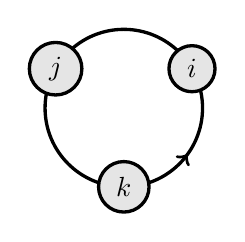
\begin{tikzpicture}[scale=1,very thick,decoration={
    markings,
    mark=at position 0.4 with {\arrow{>}}}
    ] 
  
  \draw[postaction={decorate}] (0:0)   circle (-1);
  \fill (30:1)  node[circle,draw,fill=black!10] {$i$}
        (150:1) node[circle,draw,fill=black!10] {$j$}
        (270:1) node[circle,draw,fill=black!10] {$k$};
\end{tikzpicture}
}
\end{center}
    
    \item An {\bf octonion} is an objects of the form $a+bi+cj+dk+el+fm+gn+ho$ with $a,\dots,h\in\mathbb{R}$ and $e_0=1, e_1=i, \dots, e_7=o$
    \begin{align}
        e_ie_j=\left\{\begin{array}{ll}
                e_j, & \text{if }i=0  \\
                e_i, & \text{if }j=0  \\
                -\delta_{ij}e_0 + \varepsilon_{ijk}e_k & \text{otherwise}
                \end{array}
                \right.
    \end{align}
\end{itemize}
\end{definition}

\begin{center}
\resizebox{2.5cm}{2cm}{
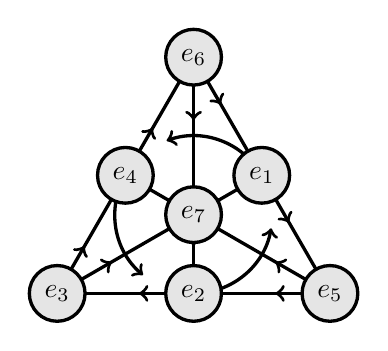
\begin{tikzpicture}[scale=1,very thick,decoration={
    markings,
    mark=at position 0.4 with {\arrow{>}}}
    ] 
  \draw[postaction={decorate}] (90:2)  --  (30:1);
  \draw[postaction={decorate}] (30:1)  --  (330:2);
  \draw[postaction={decorate}] (330:2)  --  (270:1);
  \draw[postaction={decorate}] (270:1)  --  (210:2);
  \draw[postaction={decorate}] (210:2)  --  (150:1);
  \draw[postaction={decorate}] (150:1)  --  (90:2);
  \draw[postaction={decorate}] (90:2)  --  (0:0);
  \draw[postaction={decorate}] (0:0)  --  (270:1);
  \draw[postaction={decorate}] (330:2)  --  (0:0);
  \draw[postaction={decorate}] (0:0)  --  (150:1);
  \draw[postaction={decorate}] (210:2)  --  (0:0);
  \draw[postaction={decorate}] (0:0)  --  (30:1);
  %\draw[postaction={decorate}] (0:0)   circle (-1);
  \draw[very thick, ->] (30:1) arc (30:110:1cm);
  \draw[very thick, ->] (270:1) arc (270:350:1cm);
  \draw[very thick, ->] (150:1) arc (150:230:1cm);
  
  \fill (0:0)   node[circle,draw,fill=black!10] {$e_7$}
        (30:1)  node[circle,draw,fill=black!10] {$e_1$}
        (90:2)  node[circle,draw,fill=black!10] {$e_6$}
        (150:1) node[circle,draw,fill=black!10] {$e_4$}
        (210:2) node[circle,draw,fill=black!10] {$e_3$}
        (270:1) node[circle,draw,fill=black!10] {$e_2$}
        (330:2) node[circle,draw,fill=black!10] {$e_5$};
\end{tikzpicture}
}
\end{center}

\begin{remark}{}
$\mathbb{C}$ forms a field, $\mathbb{H}$ forms a non-commutative ring
\end{remark}

\begin{definition}{}
The {\bf conjugates}  are defined by
\begin{align}
    \bar{z}&=a-bi\\
    \bar{q}&=a-bi-cj-dk\\
    &=-\frac{1}{2}\left[q+iqi+jqj+kqk\right]\\
    \bar x &= a-bi-cj-dk-el-fm-gn-ho\\
    &=-\frac{1}{6}\left[x+(ix)i+(jq)j+(kq)k)+(le)l+(mf)m+(ng)n+(oh)o\right]
\end{align}
\end{definition}

\subsection{Groups theory}
\begin{definition}{}
For a subgroup $H$ of a group $G$ {\bf a left-coset} of the subgroup $H$ in $G$ is defined as the set formed by a distinct $g\in G$
\begin{align}
    gH=\{gh: \forall h\in H\}
\end{align}
$G/H$ denotes the set of left cosets $\{gH: g \in G\}$ of $H$ in $G$ (called coset-space).
\end{definition}

\begin{definition}{}
A subgroup $N$ of a group $G$ is called {\bf normal subgroup (Normalteiler)} $N\vartriangleleft G$ if it is invariant under conjugation by members of $G$. Meaning
\begin{align}
    gng^{-1}\in N\quad \forall g\in G\\
    gN=Ng  \quad \forall g\in G\\
    gNg^{-1}=N  \quad \forall g\in G
\end{align}
\end{definition}

\begin{definition}{}
A {\bf simple group} is a nontrivial group whose only normal subgroups are the trivial group and the group itself.
\end{definition}

\begin{theorem}
Every finite simple group is isomorphic to one of the following groups:
\begin{enumerate}
    \item $Z_p$ cyclic group of prime order
    \item $A_n$ alternating group of degree $n>4$
    \item groups of Lie type (names derived from Lie algebras with $q=p^k, m\in\mathbb{N}$
    \begin{itemize}
        \item $A_n(q)$ Special projective linear group
        \item $B_n(q), n>1$ Commutator subgroup of $SO(2n+1)$ 
        \item $C_n(q), n>2$ projective symplectic group
        \item $D_n(q), n>1$ Commutator subgroup of $SO(2n)$ 
        \item $E_6(q), E_7(q), E_8(q), F_4(q), G_2(q)$ Chevalley group
        \item $^2A_n(q^2), n>1$ Special unitary group $SU(n)$
        \item $^2B_2(2^{2m+1}))$ Suzuki Groups $Sz(2^{2m+1})$
        \item $^2D_n(q^2), ^3D_4(q^3), ^2E_6(q^2)$ Steinberg group
        \item $^2F_4(2^{2m+1}), ^2G_2(2^{2m+1})$ Ree group
    \end{itemize}
    \item 26 sporadic groups
    \begin{itemize}
        \item Mathieu groups $M_{11}, M_{12}, M_{22}, M_{23}, M_{24}$
        \item Janko groups $J_1, J_2, J_3, J_4$
        \item Conway groups $Co_1, Co_2, Co_3$
        \item Fischer groups $Fi_{22}, Fi_{23}, F_{3+}$
        \item Higman–Sims group $HS$
        \item McLaughlin group $McL$
        \item Held group $F_7$
        \item Rudvalis group $Ru$
        \item Suzuki group $F_{3-}$
        \item O'Nan group $O'N$
        \item Harada–Norton group $F_5$
        \item Lyons group $Ly$
        \item Thompson group $F_3$
        \item Baby Monster group $F_2$
        \item Fischer–Griess Monster group $F_1$
    \end{itemize}
    \item $^2F_4(2)'$ Tits group (order $2^11\cdot3^3\cdot5^2\cdot13=17,971,200$)
    \begin{itemize}
        \item sometimes called the 27th sporadic group - but belongs for $m=0$ to the family $^2F_4(2^{2m+1})'$ of commutator subgroups of $^2F_4(2^{2m+1})$
    \end{itemize}
\end{enumerate}
\end{theorem}

\begin{figure}[htp]
    \centering
    %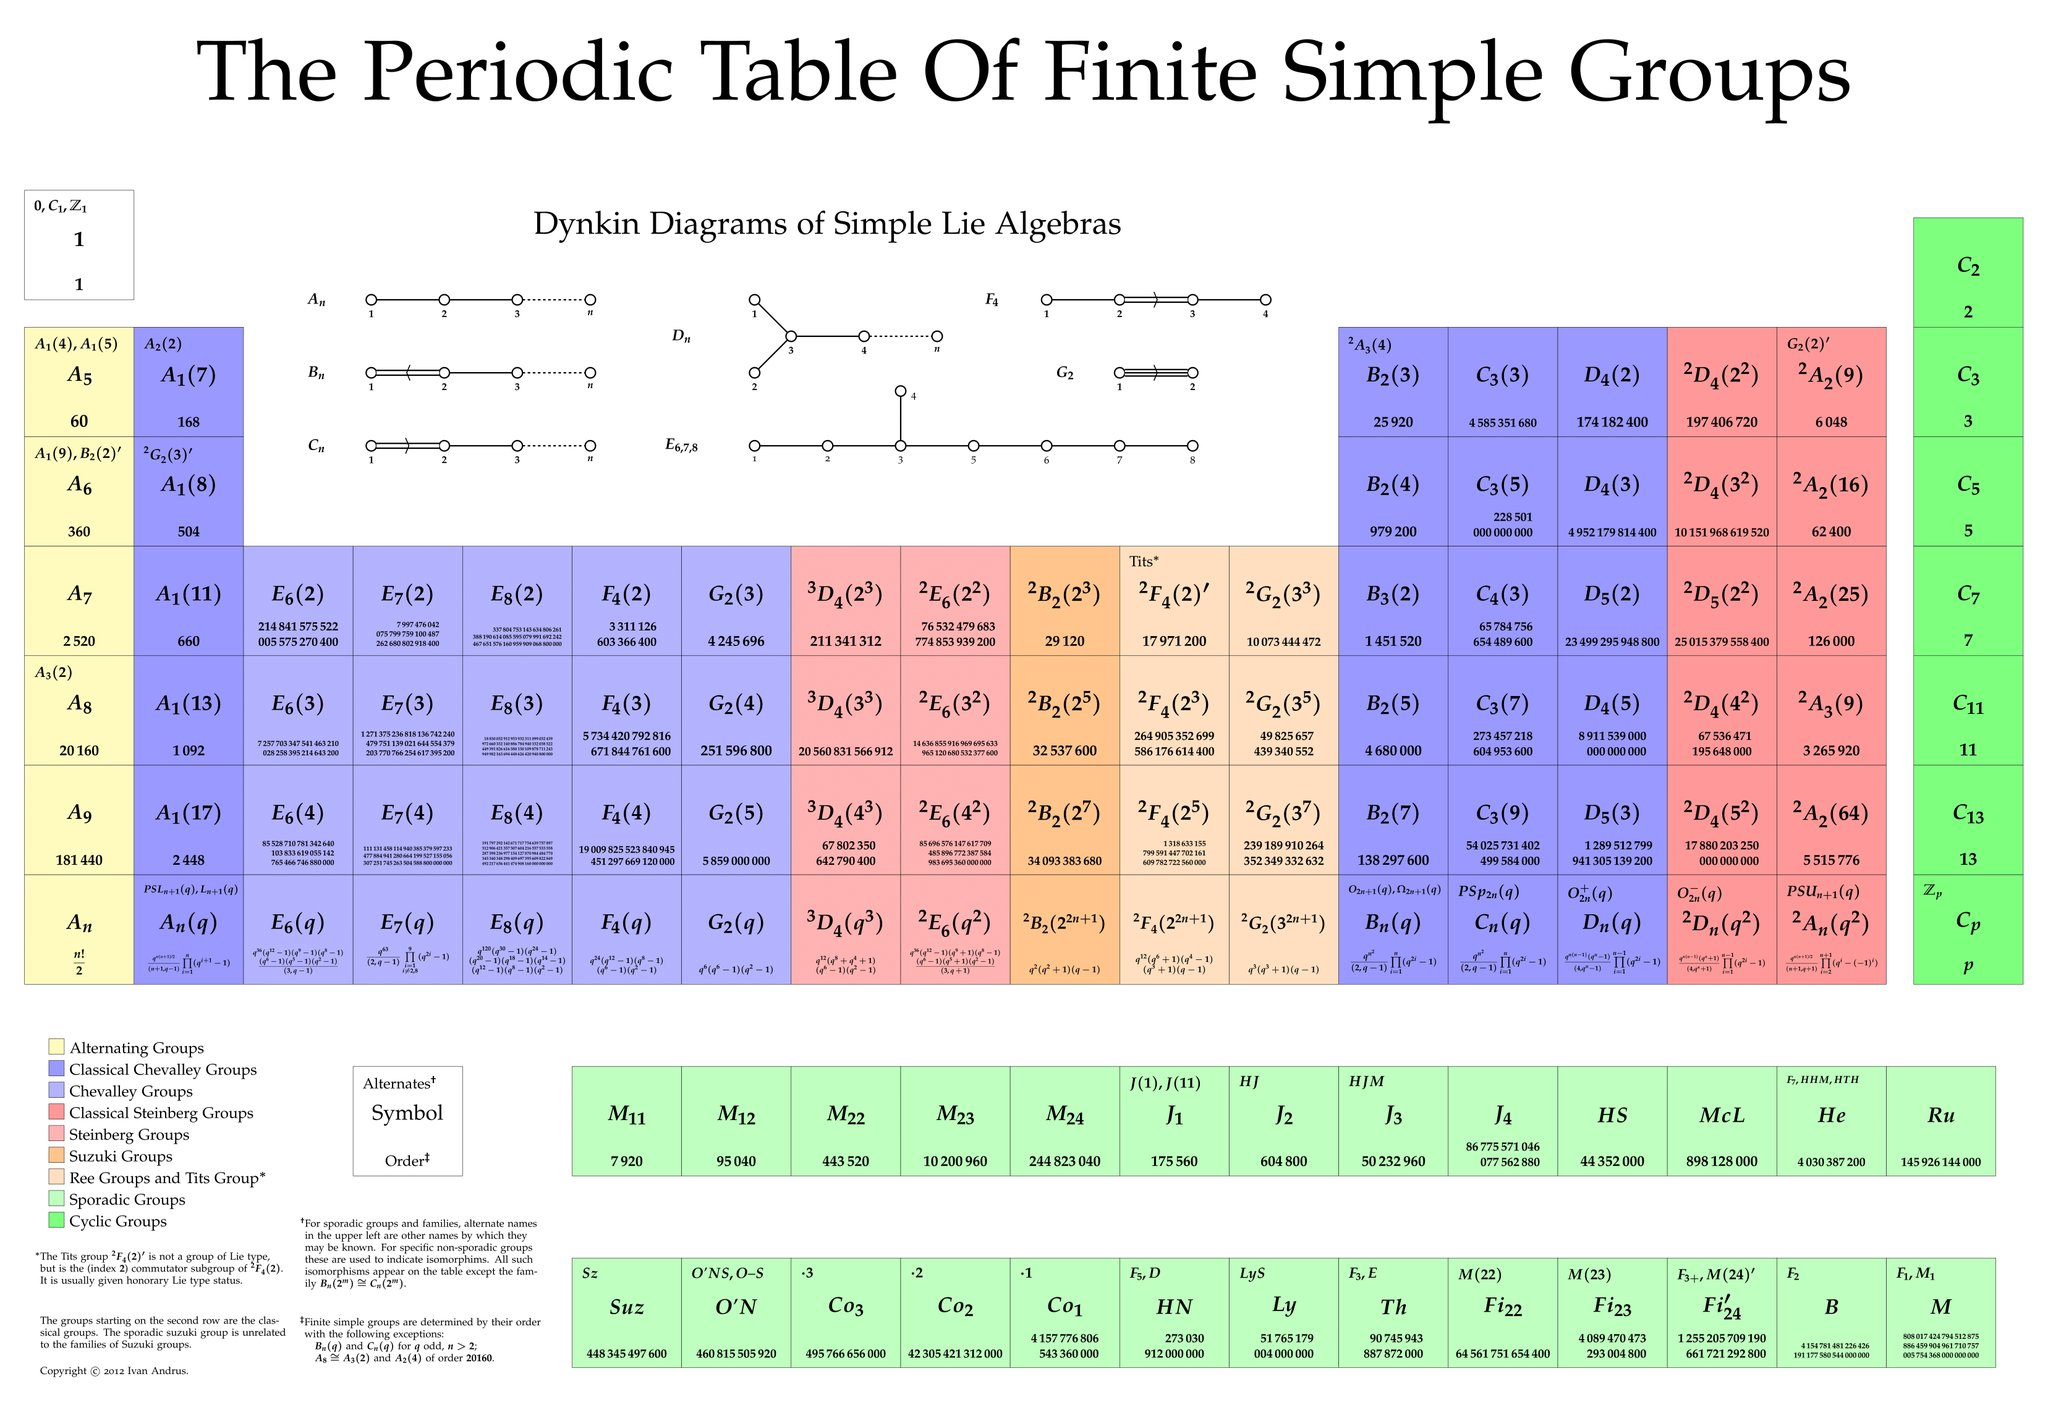
\includegraphics[width=8cm]{PTFSG.jpg}
    \caption{Periodic table of finite simple groups }
    \label{fig:galaxy}
\end{figure}

\begin{definition}{}
Exceptional Lie groups 
\begin{itemize}
    \item $G_2$ (order 14)
    \item $F_4$ (order 52)
    \item $E_6$ (order 78)
    \item $E_7$ (order 133)
    \item $E_8$ (order 248)
\end{itemize}
\end{definition}

\begin{theorem}
(Frobenius theorem, Hurwitz theorem) Any real finite-dimensional normed division algebra over the reals must be
\begin{itemize}
    \item isomorphic to $\mathbb{R}$ or $\mathbb{C}$ if unitary and commutative (equivalently: associative and commutative)
    \item isomorphic to the quaternions $\mathbb{H}$ if noncommutative but associative
    \item isomorphic to the octonions $\mathbb{O}$ if non-associative but alternative.
\end{itemize}
\end{theorem}


\begin{remark}{}
Projective spaces
\begin{itemize}
    \item $\mathfrak{so}(n+1)$ is infinitesimal isometry of the real projective spaces $\mathbb{RP}^n$
    \item $\mathfrak{su}(n+1)$ is infinitesimal isometry of the complex projective spaces $\mathbb{CP}^n$
    \item $\mathfrak{sp}(n+1)$ is infinitesimal isometry of the quaternionic projective spaces $\mathbb{HP}^n$
    \item octonionic projective line $\mathbb{OP}^1$ reproduces $\mathfrak{so}(8)$ (already accomodated by $\mathbb{RP}^7$)
    \item Cayley projective plane $\mathbb{OP}^2$ reproduces $\mathfrak{f}_4)$
    \item $\mathbb{OP}^n$ for $n>2$ gives nothing due to non-associativity of $\mathbb{O}$
\end{itemize}
\end{remark}

\begin{remark}{}
Freudenthal-Rosenfeld-Tits magic square of Lie algebras
\begin{align}
\begin{array}{c||cccc}
\mathbb{A}_1/\mathbb{A}_2 & \mathbb{R} & \mathbb{C} & \mathbb{H} & \mathbb{O}\\ \hline\hline
\mathbb{R} & \mathfrak{so}(3) & \mathfrak{su}(3) & \mathfrak{sp}(3) & \mathfrak{f}_4 \\
\mathbb{C} & \mathfrak{su}(3) & \mathfrak{su}(3)\otimes\mathfrak{su}(3) & \mathfrak{su}(6) & \mathfrak{e}_6  \\
\mathbb{H} & \mathfrak{sp}(3) & \mathfrak{su}(6) & \mathfrak{so}(12) & \mathfrak{e}_7  \\
\mathbb{O} & \mathfrak{f}_4   & \mathfrak{e}_6 & \mathfrak{e}_7& \mathfrak{e}_8 
\end{array}
\end{align}
\end{remark}



\subsection{Representation theory}
\theoremstyle{definition}
\begin{definition}{}
A {\bf representation} of a group $G=\left(\{g_i\},\circ\right)$ is a mapping $g\mapsto D(g)$ of the elements $g\in G$ onto a set of linear operators with
\begin{enumerate}
    \item $D(e)=\mathbb{I}$
    \item $D(g_1)D(g_2) = D(g_1\circ g_2)$.
\end{enumerate}
This obviously implies $D(g^{-1})=D(g)^{-1}$.
\end{definition}

\begin{remark}{}
A bit more formal - let $G$ a group and $V$ be a $\mathbb{K}$-vector space then a linear representation is a group homomorphism with
$D:G\rightarrow \GL(V)\overset{!}{=}\Aut(V)$. $V$ is then called representation space with $\dim V$ being the dimension of the representation and $D(g)\in\GL(V)$
\end{remark}

\begin{definition}{}
An {\bf equivalent representation} $D'$ of a representation $D$ is defined by 
\begin{align}
D(g)\rightarrow D'(g)=S^{-1}D(g)S   \qquad \forall g\in G
\end{align}
\end{definition}

\begin{definition}{}
A representation $D$ is called {\bf unitary representation} if 
\begin{align}
D(g)^\dagger=D(g)^{-1}    \qquad \forall g\in G
\end{align}
\end{definition}

\begin{remark}{}
For a unitary representation $D(g)^\dagger D(g)=\mathbb{I}$ an equivalent representation $D'(g)=S^{-1}D(g)S$ is only unitary
\begin{align}
    D'(g)^\dagger D'(g)&=\left(S^{-1}D(g)S\right)^\dagger S^{-1}D(g)S\\
    &=S^\dagger D(g)^\dagger (S^{-1})^\dagger S^{-1}D(g)S\\
    &=S^\dagger D(g)^\dagger (S^\dagger)^{-1} S^{-1}D(g)S\\
    &=S^\dagger D(g)^\dagger (SS^\dagger)^{-1} D(g)S
\end{align}
iff $S$ is unitary itself $SS^\dagger = \mathbb{I}$
\begin{align}
    D'(g)^\dagger D'(g)=S^{-1} D(g)^\dagger D(g)S = S^{-1} S = \mathbb{I}.
\end{align}
\end{remark}

\begin{definition}{}
A representation is called a {\bf reducible representation} if $V$ has an invariant subspace meaning that the action of any $D(g)$ on any vector of the subspace $V_P$ is still in the subspace. If the projection operator $P:V\rightarrow V_P$ projects to this subspace then
\begin{align}
PD(g)P=D(g)P   \qquad \forall g\in G
\end{align}
\end{definition}

\begin{remark}{}
$\forall |v\rangle\in V$ we have $P|v\rangle\in V_P$. If the subspace is invariant then any group action can not move it outside $D(g)P|v\rangle\in V_P$. But this means projecting it again would not change anything $PD(g)P|v\rangle = D(g)P|v\rangle$
\end{remark}

\begin{definition}{}
A representation is called an {\bf irreducible representation} if it is not reducible.
\end{definition}

\begin{definition}{}
A representation is called a {\bf completely reducible representation} if it is equivalent to a representation whose matrix elements have the form
\begin{align}
D(g)&=\left(
\begin{array}{ccc}
D_1(g) & 0      & \dots \\
0      & D_2(g) & \dots \\
\vdots & \vdots & \ddots
\end{array}
\right)
\end{align}
where all $D_j(g)$ are irreducible. Representation $D$ is is said to be the direct sum of subrepresentation $D_j$
\begin{align}
D&=D_1(g)\oplus D_2(g)\oplus\dotsi
\end{align}
\end{definition}

\begin{definition}{}
For a group of order $n$ the $n$-dimensional representation $D$ defined by 
\begin{align}
g_k&\rightarrow|e_k\rangle\\
D(g_j)|e_k\rangle&\overset{!}{=}|e_m\rangle\qquad\text{with } g_j\circ g_k=g_m\rightarrow|e_m\rangle
\end{align}
(where $\{|e_i\rangle\}$ is the ordinary $n$-dimensional cartesian basis) is called the {\bf regular representation}. The matrices are then constructed by
\begin{align}
[D(g_j)]_{ik}&=\langle e_i|D(g_j)|e_k\rangle=\langle e_i|e_m\rangle.
\end{align}
\end{definition}

\begin{theorem}
Every representation of a finite group is equivalent to a unitary representation.
\end{theorem}

\begin{theorem}
Every representation of a finite group is complete reducible.
\end{theorem}

\begin{definition}{}
Given two representations $D_1$ and $D_2$ acting on $V_1$ and $V_2$, an intertwiner between $D_1$ and $D_2$ is a linear operator $F:D_1\rightarrow D_2$ which ''commutes with $G$'' in the sense that
\begin{align}
F D_1(g) = D_2(g)F\quad \forall g \in G. 
\end{align}
\end{definition}



\section{Lie groups/algebras}
Linear representation
\begin{align}
g\to
\end{align}


\begin{remark}{}
Killing classification of simple Lie groups
\begin{itemize}
    \item SO(2n), SO(2n+1) - Lie algebra: $J^T=-J$ (skew-hermitian, trace free matrices $GL(n,\mathbb{R})$
    \item SU(n) - Lie algebra: $J^\dagger=-J$ (skew-hermitian, trace free matrices in $GL(n,\mathbb{C})$
    \item Sp(2n) - Lie algebra: $J^\dagger=-J$ (skew-hermitian matrices in $GL(n,\mathbb{H})$
\end{itemize}
\end{remark}

\section{Example representations}
\subsection{Cyclic group \texorpdfstring{$Z_2$}{TEXT}}
\begin{align}
\begin{array}{c||cc}
Z_2 & e & p \\ \hline\hline
e & e & p \\
p & p & e
\end{array}
\end{align}
\subsubsection{1d}
\begin{align}
D(e)&=1,\quad D(p)=1\\
D'(e)&=1,\quad D'(p)=-1
\end{align}

\subsection{Cyclic group \texorpdfstring{$Z_3$}{TEXT}}
\begin{align}
\begin{array}{c||ccc}
Z_3 & e & a & b \\ \hline\hline
e & e & a & b \\
a & a & b & e \\
b & b & e & a
\end{array}
\end{align}
\subsubsection{1d}
\begin{align}
D(e)=1,\quad D(a)=1,\quad D(b)=1
\end{align}
\begin{align}
D'(e)=1,\quad D'(a)=e^{i\frac{2\pi}{3}},\quad D'(b)=e^{i\frac{4\pi}{3}}
\end{align}


\subsubsection{3d - regular representation}
\begin{align}
|e\rangle=(1,0,0)^T,\quad |a\rangle=(0,1,0)^T,\quad |b\rangle=(0,0,1)^T
\end{align}
\begin{align}
D(e)=\left(\begin{array}{ccc}
1 & 0 & 0 \\
0 & 1 & 0 \\
0 & 0 & 1 
\end{array}
\right),\quad
D(a)=\left(\begin{array}{ccc}
0 & 0 & 1 \\
1 & 0 & 0 \\
0 & 1 & 0 
\end{array}
\right),\quad
D(b)=\left(\begin{array}{ccc}
0 & 1 & 0 \\
0 & 0 & 1 \\
1 & 0 & 0 
\end{array}
\right),\quad
\end{align}


\subsection{Group \texorpdfstring{$S_3$}{TEXT}}
\begin{align}
\begin{array}{c||cccccc}
S_3 & e   & a_1 & a_2 & a_3 & a_4 & a_5\\ \hline\hline
e   & e   & a_1 & a_2 & a_3 & a_4 & a_5\\
a_1 & a_1 & a_2 & e   & a_5 & a_3 & a_4 \\
a_2 & a_2 & e   & a_1 & a_4 & a_5 & a_3 \\
a_1 & a_3 & a_4 & a_5 & e   & a_1 & a_2 \\
a_1 & a_4 & a_5 & a_3 & a_2 & e   & a_1 \\
a_1 & a_5 & a_3 & a_4 & a_1 & a_2 & e \\
\end{array}
\end{align}
\begin{align}
a_1=(1,2,3),\quad a_2=(3,2,1),\quad a_3=(1,2),\quad a_4=(2,3),\quad a_5=(3, 1) 
\end{align}

\subsubsection{2d}
\begin{align}
D(e)=\left(\begin{array}{cc}
1 & 0\\
0 & 1
\end{array}
\right),\quad
D(a_1)=\left(\begin{array}{cc}
-\nicefrac{1}{2} & -\nicefrac{\sqrt{3}}{2}\\
 \nicefrac{\sqrt{3}}{2} & -\nicefrac{1}{2}
\end{array}
\right),\quad
D(a_2)=\left(\begin{array}{cc}
-\nicefrac{1}{2} & \nicefrac{\sqrt{3}}{2}\\
-\nicefrac{\sqrt{3}}{2} & -\nicefrac{1}{2}
\end{array}
\right),\\
D(a_3)=\left(\begin{array}{cc}
-1 & 0\\
0 & 1
\end{array}
\right),\quad
D(a_4)=\left(\begin{array}{cc}
\nicefrac{1}{2} & \nicefrac{\sqrt{3}}{2}\\
\nicefrac{\sqrt{3}}{2} & -\nicefrac{1}{2}
\end{array}
\right),\quad
D(a_5)=\left(\begin{array}{cc}
\nicefrac{1}{2} & -\nicefrac{\sqrt{3}}{2}\\
-\nicefrac{\sqrt{3}}{2} & -\nicefrac{1}{2}
\end{array}
\right)
\end{align}


\newpage
\section{Fun with names}
\begin{itemize}
\item Gordon vs Gordan
    \begin{itemize}
    \item {\sc Paul Gordan} (1837-1912) - Clebsch-Gordan decomposition
    \item {\sc Walter Gordon} (1893-1939) - Klein-Gordon equation
    \end{itemize}
\item Lorentz vs Lorenz
    \begin{itemize}
    \item {\sc Hendrik Lorentz} (1853-1928) - Lorentz transformation, Lorentz force
    \item {\sc Ludvig Lorenz} (1829-1891) - Lorenz gauge
    \end{itemize}
\item Hertz vs Hertz
    \begin{itemize}
    \item {\sc Heinrich Hertz} (1857-1894) - Hertzian dipole antenna
    \item {\sc Gustav Hertz} (1887-1975) - Franck-Hertz experiment
    \end{itemize}
\item Bragg vs Bragg
    \begin{itemize}
    \item {\sc William Henry Bragg} (1862-1942) - Bragg equation
    \item {\sc William Lawrence Bragg} (1890-1971) - Bragg equation
    \end{itemize}
\item Klein vs Klein
    \begin{itemize}
    \item {\sc Oskar Klein} (1894-1977) - Klein-Gordon equation, Kaluza-Klein theory
    \item {\sc Felix Klein} (1849-1925) - Klein bottle
    \end{itemize}
\item Euler vs Euler
    \begin{itemize}
    \item {\sc Hans Heinrich Euler} (1909-1941) - Euler–Heisenberg Lagrangian
    \item {\sc Leonhard Euler} (1707-1783) - Euler's formula
    \end{itemize}
\item Weyl vs Weil
    \begin{itemize}
    \item {\sc Hermann Weyl} (1885-1955) - Weyl spinor, Weyl group
    \item {\sc Andre Weil} (1906-1998) - Weil group, Chern–Weil homomorphism
    \end{itemize}
\item Jordan vs Jordan vs Jordan
    \begin{itemize}
    \item {\sc Camille Jordan} (1838-1922) - Jordan normal, Jordan-Hoelder theorem
    \item {\sc Wilhelm Jordan} (1842-1899) - Gauss-Jordan elimination
    \item {\sc Pascual Jordan} (1902-1980) - Jordan algebra, Jordan Wigner transformation
    \end{itemize}
\item Kac vs Kac
    \begin{itemize}
    \item {\sc Victor Kac} (1943-...) - Kac–Moody algebra
    \item {\sc Mark Kac} (1904-1984) - Feynman–Kac formula
    \end{itemize}
\end{itemize}
\end{document}
